\documentclass[]{memoir}          % for double sided format
\usepackage{graphics}
\usepackage{graphicx}
\usepackage{nicefrac}
\usepackage{graphicx}
\usepackage{epsf}
\usepackage{rotating}
\usepackage{array}
\usepackage{wrapfig}
\usepackage{multicol}
\usepackage{verbatim}
\usepackage{type1cm}
\usepackage[spanish]{babel}
\usepackage[utf8]{inputenc}
\usepackage{eso-pic}
\usepackage{color}
\usepackage{wallpaper}
\usepackage{appendix}
\usepackage{enumitem}
\usepackage[T1]{fontenc}
\usepackage[osf]{mathpazo}
\linespread{1.05}         % Palatino needs more leading (space between lines)
\usepackage[sort&compress,numbers,super]{natbib}      % Important to have nice sorted references, like [3-5,9]
% \usepackage{breakcites}
\usepackage{xspace}  %this package interprets the space after the symbols correctly, so there is no space if I put a comma, and there is one if I put another word after the symbol.
%\usepackage{tikz}
%\usetikzlibrary{shapes,decoration}
\usepackage{booktabs}
\usepackage{textcomp}
% \usepackage{natbib}
\usepackage{chapterbib}
\usepackage{color,soul}
\usepackage{xcolor}
% \usepackage{siunitx}


% set up a figure environment
\newenvironment{figg}
  { \begin{minipage}{.95\textwidth}
    \begin{centering}
  } 
  { %\noindent\makebox[\linewidth]{\rule{0.75\textwidth}{0.4pt}}
    \end{centering}
    \end{minipage}
  }



%%% To create boxes
 \usepackage{newfloat}
% \usepackage{caption}
\usepackage[font=footnotesize,labelfont=sc,margin={10pt,10pt},width=.75\textwidth] {caption}
% \usepackage[justification=raggedleft]{floatrow}
\DeclareFloatingEnvironment[fileext=frm,placement={!ht},name=Frame]{myfloat}
 \usepackage[framemethod=TikZ]{mdframed}
 \usepackage{multicol}
%  \usepackage[colorlinks=true]{hyperref}
 
 \newenvironment{frameenv}[1]
     {\begin{myfloat}[tb]
     \begin{mdframed}[roundcorner=10pt,backgroundcolor=blue!10]
     \caption{#1}
     \begin{multicols*}{2}
     }
     {\end{multicols*}\end{mdframed}\end{myfloat}
     }
%%% end boxes



%%%%%%%%%%% Macros by L Concha
%\newcommand{name}[num]{definition}
\newcommand{\Bzero}{$B_0$\xspace}
\newcommand{\Bone}{$B_1$\xspace}
\newcommand{\M}{$\boldsymbol{M}$\xspace}
\newcommand{\Mzero}{$\boldsymbol{M_0}$\xspace}
\newcommand{\Mx}{$\boldsymbol{M_x}$\xspace}
\newcommand{\My}{$\boldsymbol{M_y}$\xspace}
\newcommand{\Mz}{$\boldsymbol{M_z}$\xspace}
\newcommand{\Mxy}{$\boldsymbol{M_{xy}}$\xspace}
\newcommand{\omegazero}{$\omega_0$\xspace}
\newcommand{\Tone}{$T_1$\xspace}
\newcommand{\Ttwo}{$T_2$\xspace}
\newcommand{\Ttwostar}{$T_2\text{*}$\xspace}
\newcommand{\Ttwop}{$T_2'$\xspace}
\newcommand{\FA}[0]{{\sc fa}\xspace}
\newcommand{\ADC}[0]{{\sc adc}\xspace}
\newcommand{\Dunits}{$\times10^{-3} mm^{2}/s$}
\newcommand{\lone}[0]{$\lambda$$_1$\xspace}
\newcommand{\ltwo}[0]{$\lambda$$_2$\xspace}
\newcommand{\lthree}[0]{$\lambda$$_3$\xspace}
\newcommand{\lpar}{$\lambda$$_\parallel$\xspace}
\newcommand{\lperp}{$\lambda$$_\perp$\xspace}
\newcommand{\degrees}{\ensuremath{^\circ}}
\newcommand{\espaciok}{espacio $k$\xspace}
\newcommand{\kx}{$k_{x}$}
\newcommand{\ky}{$k_{y}$}
\newcommand{\figurapendiente}{\textbf{\textcolor{red}{Figura pendiente}}}
%\newcommand{\figurapendiente}{\hl{Figura pendiente}}


\setcounter{secnumdepth}{4}


% %%%% Boxes
\tikzstyle{nicebox}=[draw=gray!100, fill=blue!10, very thick,rounded corners, rectangle, inner sep=4pt, inner ysep=16pt]
\tikzstyle{niceboxtitle}=[draw=gray!100, fill=white, text=black, rounded corners, very thick, rectangle]
\newcommand\nicebox[2]{
  {\centering
  \begin{tikzpicture}
	\node [nicebox](box){
	  \begin{minipage}{0.95\textwidth}
	  \begin{minipage}{0.95\textwidth}#2
	  \end{minipage}\end{minipage}};
	\node[niceboxtitle, right=10pt] at (box.north west){\small\textbf{#1}};
\end{tikzpicture}\par}
}



%%%%%% Llamar al glosario


%%%%%%%%%%%%%%%%%%%%%%%%%%%%%%%%%%%%%%%%%%%%%%%%%% Glosario
\usepackage[toc,style=long3col,footnote,acronym]{glossaries} 
\usepackage{index}
\makeindex  
\makeglossaries

%%% GLOSARIO

\newglossaryentry{espacio k} {name={espacio k}, description={Mafufo espacio donde existen números imaginarios}}
\newglossaryentry{gradiente} {name={gradiente},
                              plural={gradientes},
                              description={Modificación lineal del campo magnético mediante electroimanes secundarios que aumentan o disminuyen el campo magnético principal de manera predecible. Usualmente en el orden de 20-60 mT/m}}


\newglossaryentry{precesion} {name={precesión},
                            description={Cambio de la orientación del eje de un cuerpo que se encuentra en rotación}}

\newglossaryentry{constanteGiromagnetica} {name={constante giromagnética},
                            description={Propiedad de una especie atómica de precesar a cierta frecuencia en cierto campo magnético}}
 % Abrevs.


\newacronym{DTI}{DTI}{diffusion tensor imaging}

%%%%%%%%%%%%%%%%%%%%%%%%%%%%%%%%%%%%%%%%%%%%%%%%%%%%%%%%%%%%%%


%%%%%% Llamar mis estilos
% para poner números atómicos bien.
\usepackage[version=3]{mhchem}






%\usepackage[svgnames]{xcolor}
\definecolor{azulUNAM}{cmyk}{100, 59, 0, 69}
\definecolor{oroUNAM}{cmyk}{0, 14, 48, 44}
\definecolor{migris}{rgb}{0.5, 0.5, 0.5}
\definecolor{minegro}{rgb}{0,0,0}


%%%%%%%%%%%%%%%%%%%%%%%%%%%% MACRO FOR CHAPTER STYLE, FROM THE MEMOIR CLASS
% SEE http://www.tex.ac.uk/tex-archive/info/MemoirChapStyles/MemoirChapStyles.pdf
\chapterstyle{veelo}

\renewcommand*\prechapterprecis{\begin{flushright}}
\renewcommand*\postchapterprecis{\end{flushright}\vskip 2cm}
%\renewcommand{\precisfont}{\scshape}
%\renewcommand{\precistocfont}{\noindent} 
%\renewcommand*\precisfont{\scshape}
%\renewcommand*\precistocfont{\scshape}

%%%%%%%%%%%%%%%%%%%%%%%%%%%%%%%%%%%%%%%%%%%%%%%%%%%%%%%%%%%%%%%%%%%%%%%%%%%%%%%%%%

%%% Change the title appearance
%\title{Imagenología por Resonancia Magnética}
%\author{Luis Concha, Fernando Barrios, Roberto Mercadillo (Editores)}
\newcommand*{\titleTH}{\pagestyle{empty}\begingroup% T&H Typography
\raggedleft
\vspace*{\baselineskip}
{\Large Luis Concha \\(Editor)}\\[0.167\textheight]
{\bfseries Imagenología por}\\[\baselineskip]
{\textcolor{minegro}{\Huge RESONANCIA MAGNÉTICA}}\\[\baselineskip]
%{\textcolor{minegro}{\small Con 123 Figuras}}\par
\vfill
%
\includegraphics[width=2cm]{logoUNAM}
%\medskip
Versión: \today \par
\vspace*{3\baselineskip}
\endgroup}
%%% end title style



%%%% part style
\renewcommand{\partnamefont}{\scshape\huge\raggedleft\thispagestyle{empty}}
\renewcommand{\partnumfont}{\scshape\huge}



% Referencias
% \usepackage[usenames]{color}
% \usepackage[hypertex,dvipdfm,pagebackref=true]{hyperref}
\usepackage[hypertex,pagebackref=true]{hyperref}
\renewcommand*{\backref}[1]{}
\renewcommand*{\backrefalt}[4]{%
      \ifcase #1 %
         {\scriptsize (no citado)}%
      \or
         {\scriptsize (Citado en p.~#2.)}%
      \else
         {\scriptsize (Citado en pp.~#2.)}
      \fi}


%%%% Captions
\captiontitlefont{\itshape\small}
\captionnamefont{\scshape\small}

 
% on tan las figuras
\graphicspath{{/home/lconcha/Documents/libroResonancia/figs/}}




\begin{document}

%\maketitle
\titleTH
\newpage

\frontmatter
\tableofcontents
%\listoftables  % if you have any
% \listoffigures % if you have any













%%%%%%%%%%%%%%%%%%%%%%%%%%%%%%%%%%%%%%%%%%%%%%%%%%%%%%%%%%%%%%%%%%%%%%%%%%%%%%%%%%%%%%%%%%%%%
\mainmatter
\pagestyle{companion}


\part{Principios básicos\\de resonancia magnética}
\label{part_principiosBasicos}


\chapter{Introducción general a la resonancia magnética}
\chapterprecis{\noindent Luis Concha\\Instituto de Neurobiología\\UNAM, Campus Juriquilla}
\label{chapter_introGeneral}
A diferencia de la mayoría de los métodos de imagen, basados en la absorbancia o reflectancia de ondas electromagnéticas como los Rayos X, la resonancia magnética se basa en principios físicos y matemáticos que pueden ser intimidantes de inicio. Mientras que en otros métodos la imagen es obtenida casi directamente, las imágenes por resonancia magnética son construidas a partir de la decodificación de múltiples señales. Sin embargo, una vez que son comprendidas ponen de manifiesto la enorme inventividad del ser humano al llevar tan altos niveles de abstracción a algo tan útil como lo es la generación de imágenes del cuerpo humano. Pocas técnicas reúnen tantos conceptos en áreas tan diversas como la física clásica y cuántica, las matemáticas, el proceso de señales y la estadística, como lo hace la imagenología por resonancia.

Comprender a fondo la manera en que se generan las imágenes de resonancia no es trivial, y requiere conocer los fundamentos de las diversas áreas que se reúnen en esta metodología. Todos los conceptos están inevitablemente encadenados y poseen un grado de complejidad jerárquica. A pesar de esto, existe una gran ventaja: en innumerables ocasiones los conceptos avanzados ayudan a afianzar los conocimientos de los conceptos que les preceden. Debemos notar que sería muy difícil, si no imposible, aprender los conceptos avanzados teniendo unas bases débiles, pero no es raro que el estudiante de resonancia magnética pueda imaginar cada vez mejor los fundamentos conforme avanza en su estudio.

Iniciaremos nuestro recorrido por la resonancia magnética dando una vista a vuelo de pájaro sobre los conceptos que participan en la generación de imagen, desde el nivel atómico hasta la visualización de la misma. La intención es proveer una visión global sobre la manera en que los conceptos se encadenan, señalando únicamente los principios fundamentales. Para quien se inicia en resonancia magnética, este capítulo pretende servir como brújula, y es labor de los siguientes capítulos de la Parte \ref{part_principiosBasicos} de este libro, el llenar los huecos y ofrecer más detalles. 


\section{Fenómeno de resonancia magnética nuclear}
Todos los átomos con un número impar de protones y/o neutrones en su núcleo poseen un spin distinto de cero. Estos núcleos se comportan como pequeñísimos imanes, con sus respectivos polos Norte y Sur. Estos imanes no se encuentran inmóviles, sino que se encuentran rotando (como lo hace nuestro planeta), y la velocidad a la que rotan (su frecuencia) es dependiente del campo magnético que están experimentando. Más correctamente, los átomos experimentan un movimiento de \index{precesión} \gls{precesion} en torno a la orientación del campo magnético local (Figura \ref{fig:spins}, A), cuya frecuencia es dependiente del mismo. Si el átomo está flotando en un medio con un campo magnético bajo, precesará a una frecuencia baja; si está inmerso en un campo magnético poderoso, precesará a una alta frecuencia. A esta relación se le conoce como la frecuencia de Larmour y es explorada en más detalle en el Capítulo \ref{chapter_fenomeno}. Sin embargo, no todos los átomos precesan a la misma frecuencia estando en el mismo campo magnético. Cada especie atómica tiene una ``firma'', una frecuencia a la que precesa dependiendo del campo magnético, y que la distingue de todas las otras especies atómicas. Esta firma se conoce como la \index{constante giromagnética} \gls{constanteGiromagnetica} y se simboliza con la letra $\gamma$. Por ejemplo, la constante giromagnética del hidrógeno es alrededor de 42.5 MHz/T, lo que nos dice que si un átomo de hidrógeno está en un campo magnético de un Tesla, dará 42.5 millones de vueltas en un segundo. Si ahora ponemos ese átomo en un campo magnético de 3 Teslas, precesará a una frecuencia de 127.5 MHz. Como el hidrógeno es el elemento más abundante en los seres vivos, es el átomo explotado para la realización de imágenes por resonancia magnética \footnote{No es el único, habiendo ejemplos notables de imagen utilizando el sodio.}. Habiendo solamente un protón en el núcleo del hidrógeno, en la mayoría de los textos de resonancia magnética, y en este en particular, es frecuente la utilización indistinta de los términos ``núcleo'', ``protón'' y ``spin'' para referirse al núcleo del átomo de hidrógeno.

\begin{figure}[htb]
 \centering
 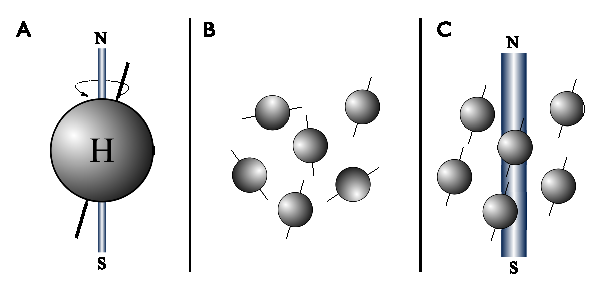
\includegraphics{spins}
 \caption{Los spins se orientan de acuerdo al campo magnético que experimentan y precesan alrededor de él (A). En el caso de un campo magnético poco potente, los spins estarán orientados aleatoriamente (B), mientras que si experimentan un campo magnético de gran intensidad, se alinearán acordemente (C).}
 \label{fig:spins}
\end{figure}



Imaginemos ahora un sencillo escenario: disponemos de una muestra de agua pura sobre una mesa cualquiera. Si analizáramos la orientación de los polos magnéticos de todos los núcleos de hidrógeno que tenemos, éstos apuntarían en diversas direcciones. Facilita la visualización si imaginamos pequeños imanes de barra orientados aleatoriamente (Figura \ref{fig:spins}, B). Si ahora colocamos nuestra muestra dentro de un campo magnético potente y analizamos nuevamente sus orientaciones, veremos que ahora todos estos imanes de barra apuntan en la misma dirección (Figura \ref{fig:spins}, C). Si recordamos que las brújulas apuntan hacia el Norte, a menos que las pongamos frente a un campo magnético aun más potente que el terrestre \footnote{1 Tesla = 10 000 Gauss. El campo magnético terrestre es de solamente 0.5 Gauss.}, no resulta soprendente que ahora todos estos imanes de barra apunten en la dirección del campo magnético que ahora experimentan. No solamente apuntan en la misma dirección, sino que también todos precesan a la misma frecuencia al estar todos experimentando el mismo campo magnético. Ahora, prendamos un campo magnético adicional pero, a diferencia del primero, éste está dando vueltas alrededor de nuestra muestra a la misma frecuencia que la que están precesando los spins (frecuencia de Larmour). Esto en la práctica es una radiofrecuencia.  Ahora nuestros pequeños imanes tienen un nuevo lugar a donde voltear y, a pesar de que este nuevo campo magnético en rotación es más débil que el primero, les resulta más atractivo, porque precesa a la misma frecuencia que ellos. Si hemos hecho que nuestro campo magnético rotatorio (radiofrecuencia) gire en un plano transversal al campo magnético principal, nuestros spins ahora querrán voltearse sobre este plano, efectivamente desviándose de la orientación del campo magnético principal. Qué tanto logren este cometido dependerá de qué tanto tiempo dejemos prendida nuestra radiofrecuencia. Además, en cuanto apaguemos nuestra radiofrecuencia, los spins ahora solo verán el campo magnético principal y regresarán a alinearse con él. Durante esta realineación los spins emitirán de regreso el exceso de energía que absorbieron de la radiofrecuencia, y lo harán a la misma frecuencia. De aquí el nombre de \emph{resonancia}, y ya hemos visto de donde provienen los términos \emph{magnética} y \emph{nuclear} (si bien en general se evita decir esta última palabra para evitar pensar en fenómenos de radiación). Este fenómeno que acabamos de describir es la base que permite la espectroscopía e imagenología por resonancia magnética, pero hace falta saber cómo explotarlo para poder traducirlo.



\section{Codificación espacial}
\label{sec_codificacionEspacial}
Hemos recibido una señal que nos han regresado las moléculas de agua de nuestra muestra gracias al fenómeno de resonancia magnética. Por supuesto que la magnitud de esta señal irá en relación directa con la cantidad de átomos de hidrógeno, y con esto tenemos una manera muy complicada y costosa para medir cuánta agua hay en nuestra muestra. Si bien en el caso de agua el ejercicio sería ridículo, este es el principio que rige la espectroscopía, que logra medir la concentración de diversas moléculas en una mezcla (Capítulo \ref{chapter_espectro}). Pero notemos una gran ventaja que tenemos: la frecuencia de resonancia depende directamente del campo magnético que experimentan los spins. Hasta ahora habíamos puesto nuestra muestra en un campo magnético homogéneo, provocando que todos los spins resonaran a la misma frecuencia. ¿Qué pasará entonces si introducimos variaciones en la potencia del campo magnético que sean dependientes de su lugar en el espacio? Los spins precesarán a distinta frecuencia, las cuales nos informarían acerca de la potencia del campo magnético que están experimentando. Dado que nosotros hemos introducido la perturbación en el campo magnético, hemos logrado codificar la posición espacial de los spins, al menos en una dimensión (Figura \ref{fig:gradientesSimple}). Las bobinas (o imanes secundarios) llamados de gradiente son los responsables de sumar o restar la potencia del campo magnético principal, logrando variaciones en el orden de los mT/m (por ejemplo, un gradiente capaz de generar 40 mT/m, variará el campo magnético principal 4 mT a lo largo de 10 cm). La manera en que la segunda dimensión es codificada es similar, pero mediante el uso de la fase del spin (hacia dónde voltea el spin si lo vemos desde arriba) y es explicada en detalle en el Capítulo \ref{chapter_espacial}.

\begin{figure}[htb]
 \centering
 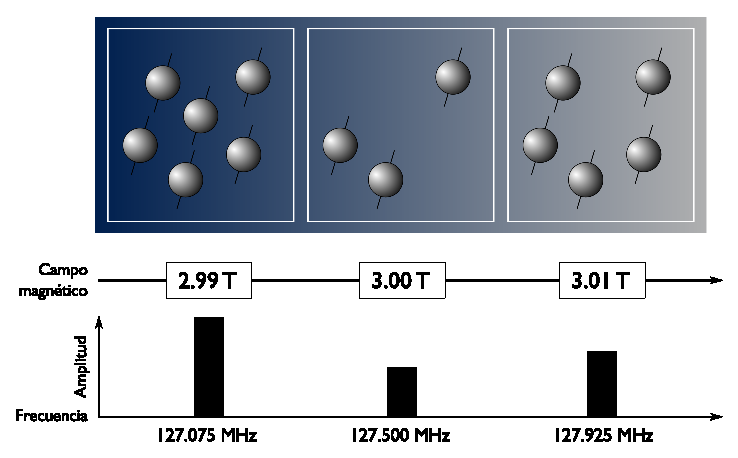
\includegraphics{gradientesSimple}
 \caption{Codificación espacial. Tres muestras, cada una con cantidades distintas de átomos de Hidrógeno, experimentan un campo magnético que aumenta en intensidad de izquierda a derecha. Cada muestra resonará a distinta frecuencia, y la amplitud de la misma dependerá de la cantidad de átomos que contiene.}
 \label{fig:gradientesSimple}
\end{figure}




\section{Secuencias de pulsos}

 Como hemos visto, los ingredientes para generar una imagen son los pulsos de radio-frecuencia y los gradientes del campo magnético y, aplicados en diversos momentos con duraciones específicas, logran imágenes con características específicas. La receta que utiliza estos ingredientes, en los tiempos y duraciones adecuadas, se denomina secuencia de pulsos. Suelen ser representadas mediante una línea de tiempo en la cual suceden los eventos, y los parámetros que las definen son precisamente los intervalos de tiempo entre ellos, o la intensidad de los mismos. Por ejemplo, el tiempo que transcurre entre dos excitaciones sucesivas de los spins se conoce como tiempo de repetición, o TR. La secuencia de pulsos para nuestro simple experimento de la Sección \ref{sec_codificacionEspacial} se ilustra en la Figura \ref{fig:secuenciaSimple}.

\begin{figure}[htb]
 \centering
 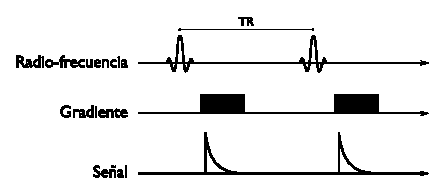
\includegraphics{secuenciaSimple}
 \caption{Secuencia de pulsos con codificación espacial en una sola dimensión (2 repeticiones).}
 \label{fig:secuenciaSimple}
\end{figure}




\fancybreak{* * *}


Con esta vista preliminar y caricaturesca, hemos logrado llevar el fenómeno de resonancia magnética hasta una imagen (al menos en una dimensión). Hemos obviado muchos detalles que contribuyen a la formación de la imagen, y no hemos tratado puntos esenciales como los fenómenos de relajación (Capítulo \ref{chapter_relajacion}), fundamentales para la existencia de contraste en una imagen. Mediante el uso juicioso de ingeniosas secuencias de pulsos, podemos hacer que los spins ``bailen el son que queramos``, lo que hace a la imagenología por resonancia magnética una de las técnicas mas poderosas y flexibles para la obtención de distintos tipos de información de una manera no invasiva (ver Parte \ref{part_protocolos}). El resto de los capítulos de la Parte \ref{part_principiosBasicos} brindan más información sobre aspectos específicos de estos interesantes temas.


% \bibliographystyle{concha2}
% % \bibliography{libroResonancia}



\chapter{Aspectos históricos de la resonancia magnética}
\chapterprecis{\noindent Giovanna Lilian Licea Haquet\\Instituto de Neurobiología\\UNAM, Campus Juriquilla}
\label{chapter_historia}

La técnica de  resonancia magnética y la aplicación clínica que tiene hoy en día es resultado de años de investigación de diferentes grupos de investigación, y es el ejemplo de cómo los esfuerzos de la investigación básica pueden llegar a tener después de un tiempo un rango alto de aplicabilidad.
La resonancia magnética surgió como resultado de la investigación de la naturaleza de la materia, en este campo, un hallazgo importante fue el de Pauli, físico austriaco que en los años veinte propuso el cuarto número cuántico: el spin del electrón y la existencia del spin nuclear, demostró que muchas de las características de la estructura hiperfina de los espectros atómicos se podían explicar si los núcleos atómicos presentaban spin, que es una partícula giratoria que genera un campo magnético y un momento magnético asociado y actúa como una pequeña barra magnética con polos positivo y negativo. Si se coloca una átomo en un campo magnético externo potente, el momento magnético de su núcleo tiende a alinearse con (en paralelo) o contra (en sentido antiparalelo) el campo externo \cite{Canals_2008}.

Durante la década de 1930 Isidor Isaac Rabi, profesor de la Universidad de Columbia, junto con su equipo de investigación utilizaba una técnica denominada resonancia de haces moleculares para estudiar las propiedades magnéticas de los átomos y las moléculas. En 1939, y por consejo  del físico holandés Cornelius J. Gorter,  quien había intentado medir la resonancia magnética de núcleos de Li en LiCl sólido mediante técnicas microcalorimétricas sin resultados favorables, añadió ondas de radio a los haces moleculares mientras variaba la potencia del campo magnético y encontró que con el estímulo apropiado, los momentos magnéticos de los núcleos podían invertirse o cambiar su orientación en relación al campo magnético absorbiendo energía de la señal de radio. Posteriormente hizo experimentos variando la frecuencia de radio en lugar de la potencia del campo magnético, y descubrió que de esta manera se amplía el espectro de las señales resultantes y el espectro de la luz visible. Este método se convirtió en la base de la espectroscopia de radiofrecuencias, que revolucionó el análisis químico y es un componente esencial en el desarrollo de las exploraciones mediante resonancia magnética como herramienta de diagnóstico médico. El aporte que hicieron sus descubrimientos le valieron a Rabi el premio Nobel de física en 1944 \cite{Shampo2012,Canals_2008}.

Con el comienzo de la Segunda Guerra Mundial se interrumpieron las investigaciones sobre resonancia magnética nuclear \cite{Canals_2008,Luiten2003}. Al fin de ésta, en 1945, dos grupos de Estados Unidos, trabajando independientemente, intentaron  medir resonancia magnética nuclear en materia condensada, a pesar de que Gorter no lo había logrado. Uno de estos dos grupos, dirigido por E.M. Purcell, trabajaba en la Universidad de Harvard, Massachusetts. El otro, dirigido por Felix Bloch, lo hacía en la Universidad de Stanford, California. Ambos investigadores no se conocían \cite{Luiten2003}. La primera detección de resonancia magnética nuclear en materia condensada fue conseguida por el equipo de Purcell, Torrey y Pound en Harvard. El experimento consistió en situar un bloque de 850 $cm^3$ de parafina sólida, en una cavidad resonante de radiofrecuencia, alimentada a 30 MHz por medio de un circuito. Este conjunto se hallaba dentro de un electroimán de campo magnético variable. La señal de salida del resonador se balanceó en fase y amplitud con la porción de la señal de salida, y al encender el campo magnético se observó una aguda absorción por resonancia para un valor del campo de 7100 Gauss \cite{Purcell1946}. De manera completamente independiente, el equipo de Felix Bloch en Stanford consiguió, a fines 1945, detectar también señales de RMN de protón, utilizando un equipo experimental muy diferente y sobre una muestra de agua. En lugar de un único circuito de radiofrecuencia, en el experimento de Bloch se utilizaron dos bobinas mutuamente ortogonales, una para la excitación y la otra como detector; las dos bobinas se hallaban dentro de un fuerte campo magnético variable, perpendicular a ambas bobinas, con este diseño buscaba detectar sobre la segunda bobina la fuerza electromotriz inducida por la precesión de la magnetización nuclear de la muestra, provocada por la primera bobina al producirse la absorción \cite{Bloch1946}. En 1952, Bloch y Purcell compartieron el premio Nobel de física por estos experimentos \cite{Detre2007}.

El siguiente avance se le debe a E. L. Hahn, quien en 1949 quien siguió la idea de Bloch de producir una corta excitación mediante un pulso de radiofrecuencia, y descubrió un fenómeno conocido como Free Induction Decay (FID), base de las secuencias usadas actualmente y de  de gran importancia para la medición de los tiempos de relajación. En un principio, Hahn atribuyó estas señales aparentemente falsas a un fallo en su equipo electrónico. Tras un estudio más profundo, reconoció que estaban causadas por la aceleración y desaceleración de los núcleos giratorios debido a las variaciones en los campos magnéticos locales. Al aplicar dos o tres impulsos de radio cortos y, a continuación, escuchar el eco, Hahn descubrió que podía obtener información aún más detallada sobre la relajación del espín nuclear de lo que era posible con un único impulso \cite{Canals_2008}.

A finales de la década de 1950, Russell Varian propuso un nuevo método de impulsos denominado resonancia magnética nuclear con transformada de Fourier. Prácticamente al mismo tiempo, Irving Lowe y Richard E. Norberg, de la Universidad de Washington en St. Louis, demostraron experimental y teóricamente cómo era posible obtener todos los resultados disponibles de los experimentos con onda continua mediante la manipulación matemática de las señales producidas en un experimento con impulsos. Sin embargo, en aquel momento el proceso matemático necesario para analizar los datos de los impulsos (transformación de Fourier) no resultaba práctico debido a las limitaciones de los equipos informáticos de la época.

En 1966 Richard R Ernst y Wess W Anderson  aplican la transformada de Fourier a la espectroscopía por resonacia magnética. Utilizando la FID de Hahn y analizando la transformada de la respuesta del sistema, aumentaron la razón señal/ruido; esta técnica abre las puertas al análisis computacional de las señales, reduciendo significativamente el tiempo de registro.  Para entonces, los avances realizados en el campo de la informática hacían que la transformada de Fourier resultara práctica. Hoy es posible emplear la resonancia magnética nuclear para analizar muestras muy pequeñas de un material o identificar átomos poco comunes en muestras más grandes. En 1991, Ernst obtuvo el premio Nobel de química por sus contribuciones al desarrollo de la espectroscopia de la resonancia magnética nuclear de alta resolución. 

Hasta ese momento, en los avances realizados en la resonancia magnética no se había pensado en utilizarla para obtener imágenes, pero comenzaban a verse aplicaciones clínicas. En 1969, Raymond Damadian, un médico del Downstate Medical Center de Brooklyn (Nueva York), comenzó a idear la forma de utilizar esta técnica para detectar los primeros signos del cáncer en el organismo. En un experimento realizado en 1970, Damadian extirpó una serie de tumores de rápido crecimiento que se habían implantado en ratas de laboratorio y comprobó que la resonancia magnética nuclear de los tumores era diferente de la de los tejidos normales. En 1971, Damadian publicó los resultados de sus experimentos en la revista Science. Sin embargo, aún no se había demostrado la fiabilidad clínica del método de Damadian en la detección o diagnóstico del cáncer \cite{Canals_2008}.

El gran avance técnico que hizo posible producir una imagen útil a partir de las señales de resonancia magnética nuclear de tejidos vivos lo realizó el químico estadounidense Paul Lauterbur en 1971, cuando observó al químico Leon Saryan repetir los experimentos de Damadian con tumores y tejidos sanos de ratas. Lauterbur llegó a la conclusión de que la técnica no ofrecía la información suficiente para diagnosticar tumores y se propuso idear un método práctico para obtener imágenes a partir de la resonancia magnética nuclear. La clave estaba en ser capaz de localizar la ubicación exacta de una determinada señal de resonancia magnética nuclear en una muestra: si se determinaba la ubicación de todas las señales, sería posible elaborar un mapa de toda la muestra \cite{Luiten2003,Jara2013}. La idea de Lauterbur consistió en superponer al campo magnético estático espacialmente uniforme un segundo campo magnético más débil que variara de posición de forma controlada, creando lo que se conoce como gradiente de campo magnético. En un extremo de la muestra, la potencia del campo magnético sería mayor, potencia que se iría debilitando con una calibración precisa a medida que se fuera acercando al otro extremo. Dado que la frecuencia de resonancia de los núcleos en un campo magnético externo es proporcional a la fuerza del campo, las distintas partes de la muestra tendrían distintas frecuencias de resonancia. Por lo tanto, una frecuencia de resonancia determinada podría asociarse a una posición concreta. Además, la fuerza de la señal de resonancia en cada frecuencia indicaría el tamaño relativo de los volúmenes que contienen los núcleos en distintas frecuencias y, por tanto, en la posición correspondiente. Las sutiles variaciones de las señales se podrían utilizar entonces para representar las posiciones de las moléculas y crear una imagen \cite{Andrew2007}. Por su parte, en 1976 Peter Mansfield, de la Universidad de Nottingham, Inglaterra, desarrolló una técnica ultrarrápida para obtener imágenes con resonancia magnética conocida como técnica ecoplanar, que es la clave para crear imágenes con resonancia magnética de forma rápida \cite{Luiten2003,Andrew2007}. 

A principios de la década de 1980, la gran oleada de investigaciones relacionadas con la obtención de imágenes por resonancia magnética dieron lugar a un floreciente sector comercial. Los avances en el campo de la informática de alta velocidad y los imanes superconductores permitieron a los investigadores diseñar máquinas de resonancia magnética de mayores dimensiones con una sensibilidad y una resolución inmensamente mejores \cite{Jara2013}.

El gran avance que condujo a la resonancia magnética funcional se produjo a principios de la década de 1980, cuando George Radda y sus colegas de la Universidad de Oxford, Inglaterra, descubrieron que con la resonancia magnética se podían obtener imágenes con contraste dependiente del nivel de oxígeno de la sangre y esto podía servir para realizar un seguimiento de la actividad fisiológica,  a estó se denominó BOLD (blood oxygen level dependent) \cite{Maestu_2008}. En 1990, Seiji Ogawa informó que en estudios realizados con animales, la hemoglobina desoxigenada colocada en un campo magnético aumentaba la potencia de dicho campo, mientras que la hemoglobina oxigenada no. Ogawa demostró en estudios con animales que una zona que contiene gran cantidad de hemoglobina desoxigenada deforma ligeramente el campo magnético que rodea al vaso sanguíneo, deformación que se ve reflejada en una imagen por resonancia magnética.

Otros investigadores comenzaron a estudiar estos efectos en seres humanos. Actualmente, las imágenes obtenidas por resonancia magnética funcional se utilizan, entre otras cosas, para guiar a los cirujanos de forma que no se dañen zonas esenciales del cerebro, para detectar síntomas de infartos cerebrales y para esclarecer el funcionamiento del cerebro \cite{Maestu_2008}.




\chapter{Fenómeno de resonancia magnética}
\chapterprecis{\noindent Luis Concha\\Instituto de Neurobiología\\UNAM, Campus Juriquilla}
\label{chapter_fenomeno}
Para comprender la manera en que se obtienen las señales que se convertirán en imágenes de resonancia magnética, debemos comenzar por comprender el fenómeno de resonancia magnética, para lo cual algunos conceptos de física elemental deben ser presentados. En un esfuerzo por mantener la claridad en la exposición de los términos, será inevitable recurrir a las imprecisiones, por lo que se recomienda que el lector interesado recurra a los libros de texto de física para ahondar en el tema.

\section{El spin nuclear}
\index{spin}
El spin (propiamente escrito como \emph{espín} en castellano, o momento angular intrínseco) es una propiedad general de las partículas. Es en realidad un fenómeno descrito mediante física cuántica, aunque es útil imaginarlo como la rotación de una partícula (protón, neutrón o electrón) sobre su propio eje y es medido en múltiplos de \nicefrac{1}{2}, con valores posibles positivos y negativos. Un par de spins con valor idéntico pero signo opuesto elimina la manifestación del mismo. Por su existencia tanto dentro como fuera del núcleo, existe un spin electrónico y un spin nuclear, siendo el segundo el que nos compete. Cuando el número combinado de protones y neutrones en el núcleo atómico es par, no existe un spin. Sin embargo, el desequilibrio entre los signos de los spins de las partículas atómicas producirá un spin nuclear neto. Por ejemplo, el núcleo del hidrógeno (\ce{^1 H}) solamente contiene un protón, por lo que el spin nuclear neto es de \nicefrac{1}{2}. La importancia de ésto reside en que en presencia de un campo magnético externo, un spin neto tiene la capacidad de absorber energía, por lo que el fenómeno de resonancia magnética solamente puede realizarse en elementos o isótopos con un spin neto distinto de cero. Afortunadamente, el \ce{^1 H} es el elemento más abundante en la materia orgánica, por lo que es el más comúnmente utilizado para la obtención de señal. No obstante, existe la posibilidad de realizar imágenes y espectroscopía por resonancia magnética a partir de otras especies atómicas, como el \ce{^2H}, \ce{^{31}P}, \ce{^{23}Na}, \ce{^{13}C}, etc.

Si el spin nuclear, $I$, es distinto a cero, existe un momento magnético asociado de acuerdo a la siguiente ecuación:
\begin{equation}
 \mu = \gamma I
\end{equation}
donde $\gamma$ representa la proporción giromagnética y se mide en unidades de frecuencia por intensidad del campo magnético (Hz/T). Muchos libros de texto utilizan radianes por segundo en lugar de Hz. \footnote{Para convertir: 1 Hz = 2 $\pi$ rad/s} En el caso de \ce{^1H}, $\gamma$ = 42.5 MHz/T. La unidad de intensidad del campo magnético se denomina Tesla (T) y equivale a 10,000 Gauss (G). Como referencias, el campo magnético de nuestro planeta, medido en el ecuador, es de 31 $\mu$T (3.1$\times$10$^{-5}$ T, o 310 mG), mientras que el campo magnético necesario para lograr que una rana levite es de 17 T \cite{Berry_Geim_1997}.

Al introducir un sistema de spins (por ejemplo, una muestra de agua) en un campo magnético potente, los momentos magnéticos de cada spin se alinean con el campo magnético externo, que llamaremos \Bzero, \index{B0} de forma paralela o anti-paralela. Esto es similar a lo que un imán de barra hace al estar en presencia de otro campo magnético, como lo hace la aguja de una brújula al alinearse con el polo Norte de nuestro planeta. En el caso de la brújula, el extremo Sur de la aguja apuntará hacia el Norte del planeta, pues es la configuración que requiere menos energía. Sin embargo, en los sistemas de spins, es posible que el momento magnético tenga una alineación anti-paralela con \Bzero. Al requerir mayor energía, la configuración anti-paralela es desfavorecida, si bien en una proporción muy pequeña, en función de la siguiente fórmula:
\begin{equation}
 \Delta E = \hbar \gamma B_0
\end{equation}
donde $\hbar$ es la constante de Planck reducida.\footnote{$\hbar$ = 6.626069$\times$10$^{-34}$ Js} Al ser $\hbar$ y $\gamma$ constantes, podemos ver que la diferencia de energía ($\Delta$E) entre las dos configuraciones de spins es directamente proporcional al campo magnético que experimentan (\Bzero). Como se dijo antes, existe una preferencia por el estado paralelo, al ser de menor energía, y podemos conocer la proporción entre el número de spins paralelos (N$\uparrow$) en relación a los spins anti-paralelos (N$\downarrow$) mediante la ecuación de Bolzmann, que va en función de $\Delta$E y la temperatura (T):
\begin{equation}
 \label{eq_Boltzmann}
 N_{\uparrow} / N_{\downarrow} = e^{-\Delta E / kT}
\end{equation}
donde $k$ es la constante de Boltzmann\footnote{1.3805$\times$10$^{-23}$ J/Kelvin}, y la temperatura se expresa en grados Kelvin. Como veremos, es la magnitud de la diferencia entre estos dos estados lo que se convertirá en la fuente de nuestra señal, así que tenemos dos opciones para maximizarla: (i) reducir la temperatura hacia el cero absoluto, o (ii) aumentar la intensidad del campo magnético \Bzero. Como los seres vivos no sobreviviríamos a temperaturas exageradamente bajas, la segunda opción es más alentadora.

Si nosotros inyectamos energía al sistema de spins, lograremos que los spins experimenten una transición entre los dos estados (cambiaremos la proporción $N_{\uparrow}/N_{\downarrow}$). Para que ésto suceda, la magnitud de la energía debe ser precisamente igual a $\Delta$E. 




\section{Equilibrio del sistema de spins en presencia de un campo magnético}
Antes de analizar las perturbaciones posibles en un sistema de spins, consideremos su situación una vez que se introduce una hipotética muestra de agua a un campo magnético potente. Primero que nada, es crucial el reconocimiento de que cuando se habla de muestras, se habla de miles de millones de moléculas, en este caso particular, muestras de agua, cada una de ellas con dos átomos de \ce{^1H}. El ensamble de spins se encuentra alineado en forma paralela o anti-paralela con \Bzero, y existe un excedente en el estado paralelo (baja energía) de acuerdo a la ecuación \ref{eq_Boltzmann}. Propagando la analogía de los spins como un imán de barra, consideremos que el momento magnético del spin es un vector alineado con \Bzero de forma paralela o anti-paralela. En el ensamble de spins, la suma vectorial de todos estos diminutos vectores se traducirán en un vector de magnitud considerable, \Mzero, que representa a todo el ensamble y que, por ende, está alineado paralelamente a \Bzero. Habitualmente nos referiremos a este vector resultante como \Mz, pues por convención se considera que \Bzero está alineado sobre el eje cartesiano $z$. Una enorme ventaja que este modelo brinda es que nos permite utilizar herramientas propias de la física clásica para explicar el fenómeno de resonancia magnética, dejando de lado las difíciles consideraciones cuánticas.

Mientras el sistema de spins experimente el campo \Bzero, \Mzero estará descansando sobre el eje $z$, con lo que \Mz = \Mzero. En realidad, el vector de magnetización \Mz no está estático, sino que describe un movimiento alrededor del eje $z$ conocido como \emph{precesión}. Este movimiento es similar al que realiza el eje magnético de nuestro planeta en relación al eje geográfico al realizar el globo su movimiento de rotación. Así como los ejes geográfico y magnético de nuestro planeta se encuentran separados por 23.5\degrees, \Mzero precesa alrededor del eje $z$ con un ángulo de 54.7\degrees. Como cada spin individual se encuentra en posiciones distintas alrededor de $z$, su suma vectorial es cero, por lo que reafirmamos que no hay componentes de \Mzero sobre $x$ o $y$. Si bien el ángulo de precesión no es muy relevante, la velocidad con la que \Mz gira alrededor de $z$ es fundamental y fácil de predecir, pues obedece una sencilla relación:

\begin{equation}
 \label{eq_Larmour}
 \omega = \gamma B_0
\end{equation}

Esta frecuencia de precesión se conoce como la frecuencia de Larmour o frecuencia de resonancia, y es el corazón de todos los métodos y aplicaciones de resonancia magnética. En general, cuando se escribe como $\omega$, se encuentra expresada en unidades de rad/s, mientras que si se escribe como $\nu$, las unidades de frecuencia son Hz, por lo que deben utilizarse las unidades correspondientes al referirse a $\gamma$. Esta sencilla ecuación nos dice, entonces, que la frecuencia de precesión de \Mzero con respecto a $z$ depende linealmente del campo magnético. Así, una muestra de agua en un resonador comercial de 1.5 T mostrará una frecuencia de precesión de  42.5 MHz/T $\times$ 1.5 T = 63.75 MHz, mientras que en un resonador de 9.4 T la frecuencia de Larmour es de aproximadamente 400 MHz. En general, los instrumentos de resonancia para realizar imagen se especifican por su intensidad de campo magnético, mientras que los potentes resonadores diseñados para espectroscopía (Capítulo \ref{chapter_espectro}) se especifican por su frecuencia de resonancia.

\section{Perturbación del sistema de spins}
Un pulso energía puede utilizarse para lograr una transición en la configuración paralela o anti-paralela de los spins, la cual debe ser precisamente la indicada por la ecuación \ref{eq_Boltzmann}. En la práctica, esta energía se aplica mediante la presencia de un pulso de radio-frecuencia (RF)\index{RF, radiofrecuencia|textbf}. Recordando que una onda electro-magnética tiene una longitud de onda y por lo tanto una frecuencia, podemos adelantar que la frecuencia de dicha onda debe coincidir exactamente con la frecuencia de resonancia. Por añadidura, una onda electro-magnética no es más que un campo magnético oscilatorio, por lo que podemos considerar a este pulso de RF como un segundo campo magnético, al que llamaremos \Bone, que gira alrededor de $z$ con una frecuencia $\omega$. En comparación con \Bzero, la intensidad de \Bone es varios órdenes de magnitud menor, pero al ser justo la que corresponde con la diferencia entre los dos estados energéticos de los spins, resulta en un efecto neto de atracción para los mismos. En términos de física clásica, podemos imaginarnos que \Mzero ahora busca alinearse con \Bone y, al estar este nuevo campo magnético en rotación, lleva a \Mzero con él en su recorrido alrededor de $z$. Con ésto, \Mzero presenta ahora proyecciones sobre el plano $x,y$ y disminuye su proyección sobre el eje $z$; la duración del pulso de RF determinará el ángulo que \Mzero presentará con respecto al eje $z$. Para fines ilustrativos, habitualmente se considera que el pulso de RF logra desviar a \Mzero 90\degrees, con lo que \Mz desaparece y \Mzero se encuentra totalmente sobre el plano $x,y$, rotando alrededor de $z$ a la frecuencia de resonancia. Al apagar el pulso de RF, \Bzero se convierte nuevamente en el atractor de los spins, con lo que \Mzero se dirige nuevamente a la situación en equilibrio. La recuperación de la situación en equilibrio no sucede instantáneamente y se ve afectada por las propiedades de la muestra mediante distintos mecanismos denominados de relajación que son abordados en el Capítulo \ref{chapter_relajacion}. Por el momento, baste señalar que la perturbación del sistema de spins tiene dos objetivos principales: Por una parte, logra colocar el vector de magnetización sobre el plano $x,y$, lo cual es crucial para poder registrar una señal (ver más adelante) y, por otra parte, obliga al sistema a sufrir los mecanismos de relajación, que serán fuente del contraste de la imagen.


\section{Obtención de la señal de resonancia}
\label{section:mrsignal}
El término \emph{resonancia} se refiere a la capacidad de los spins de absorber energía cuando ésta se encuentra en cierto rango. Sin embargo, también puede aplicarse el término para referirse a la manera en que el sistema de spins se deshace del exceso de energía, devolviendo la RF a la que fue expuesto. Para poder registrarla, se debe contar con una bobina, o antena, colocada alrededor del plano $x,y$, la cual sufrirá una fuerza electro-motriz en respuesta al movimiento oscilatorio de \Mzero que precesa alrededor de $z$ después de haber sido perturbado. La fuerza electromotriz se produce por la ley de inducción de Faraday, que dice que una partícula eléctrica en movimiento produce un campo magnético y viceversa. En este caso, tenemos un vector de magnetización, \Mzero, que oscila alrededor de $z$, acercándose y alejándose periódicamente de la bobina estática; las oscilaciones de \Mzero con respecto a la bobina inducen en ella un flujo de electrones de manera sinusoidal (teniendo ésta onda una frecuencia equivalente a la frecuencia de precesión). Evidentemente, registrar exactamente la misma frecuencia con la que excitamos el sistema sería un ejercicio futil, por lo que nos interesa la manera en que esta frecuencia se ve afectada por la muestra misma. Así, puede ser que registremos no solamente a $\omega$, sino a muchas otras frecuencias cercanas a ella que nos informarán de las características de la muestra. Estas variaciones espectrales son el vehículo de información variada, tales como la posición espacial de los spins emisores, o las características físicas de la muestra o tejido de estudio. La señal que recibimos desaparece a lo largo del tiempo, por lo que se le conoce como decaimiento libre (\textit{free-induction decay}, FID)\index{FID}. Las causas de su desapareción progresiva se detallan en el Capítulo \ref{chapter_relajacion}. 

La señal recibida es, pues, la suma compleja de muchas frecuencias, la cual debe ser descompuesta en las frecuencias subyacentes para su análisis, para lo cual se utiliza la transformada de Fourier.



% \tikzstyle{mybox} = [draw=black, fill=blue!20, very thick,
%     rectangle, rounded corners, inner sep=5pt, inner ysep=20pt]
% \tikzstyle{fancytitle} =[fill=black, text=white]
% 
% \begin{tikzpicture}
% \node [mybox] (box){%
%     \begin{minipage}{0.75\textwidth}
%         To calculate the horizontal position the kinematic differential
%         equations are needed.
%     \end{minipage}
% };
% \node[fancytitle, right=10pt] at (box.north west) {A fancy title};
% \end{tikzpicture}



\chapter{Relajación y Contraste}
\chapterprecis{\noindent Luis Concha\\Instituto de Neurobiología\\UNAM, Campus 
Juriquilla}
\label{chapter_relajacion}
En el Capítulo \ref{chapter_fenomeno} revisamos cómo un pulso de 
radiofrecuencia (RF), sintonizado a la frecuencia de Larmour $\omega_0$ es 
capaz de perturbar el momento magnético del sistema de spins (\M). Si la 
radiofrecuencia se aplica durante un tiempo determinado, podemos desviar a \M
a nuestro gusto. A esto le llamamos 
\textit{excitación}. Si provocamos una desviación de 90\degrees, \M
pasará de estar totalmente en el eje $z$ (\Mz=\M) al plano $x,y$, mientras que una  desviación de menos de 90\degrees ($\alpha$\degrees) colocará una fracción de \M en el plano $x,y$ (específicamente, $\sen(\alpha)$).

Una vez que el pulso de RF se apaga, el sistema de spins tenderá a regresar a 
su estado de reposo, es decir, sobre el eje $z$ (alineado con \Bzero). Este 
regreso al estado de reposo se conoce como \textit{relajación} y es la causa principal por la que nuestra señal es abundante al principio y progresivamente desaparece en un decaimiento libre (\textit{free-indiction decay}, FID)\index{FID}. Mientras  \M tenga una proyección sobre el eje $x,y$, estaremos recibiendo señal de resonancia, y ésta última irá decayendo poco a poco, porque \M estará regresando a apuntar al eje $z$, disminuyendo progresivamente su proyección en el eje $x,y$. Si tuviéramos una muestra exclusivamente de 
Hidrógeno (sin impurezas), en un campo magnético perfectamente homogéneo, todos 
los átomos de \ce{^1H} se relajarían al mismo ritmo, emitiendo señal perfectamente 
sintonizada a $\omega_0$. Esto sería un experimento aburrido, pues la RF que 
inyectamos, sintonizada a $\omega_0$ sería exactamente la misma que 
recibiríamos. Afortunadamente, en el mundo real no sucede así, y la relajación 
de diferentes tejidos sucede a diferentes velocidades. Al realizar la obtención 
de la señal, podemos permitir que pase cierto tiempo a partir de la excitación, 
con lo que permitiremos que los diferentes tejidos se relajen en distintas 
proporciones. La señal que recibiremos de cada uno de ellos será 
distinta: algunos tejidos se habrán relajado tanto que su proyección en el 
plano $x,y$ será casi nula, mientras que aquéllos que tarden mucho en relajarse 
podrán emitir mucha señal. A esta diferencia de intensidad de señales se le 
conoce como \textit{contraste}, y en términos de imagen provoca que algunos 
pixeles sean más brillantes que otros.

Existen dos fenómenos de relajación  que son independientes, pero que 
suceden simultáneamente. Esto en ocasiones provoca confusión, pero es análogo a 
lo que sucede con los fenómenos de rotación y traslación de nuestro planeta.


\section{Marco de referencia en rotación}
Antes de hablar de relajación es conveniente presentar un truco que hará mucho más fácil la descripción de un sistema de spins que se relaja. Hasta ahora, hemos considerado que al aplicar el pulso RF nuestro vector \M se alineará con \Bone, que oscila a la misma frecuencia de precesión. Es decir, \Bone da vueltas alrededor del eje $z$, y \M voltea a verlo, también dando vueltas. Con el tiempo, la trayectoria de \M al ser perturbado por el pulso de RF dibujaría una espiral descendente, resultado de sumar la precesión a la excitación, que hace pasar a \M del eje $z$ al plano $x,y$. A este punto de vista le llamamos el \textit{marco de referencia del laboratorio} \index{marco de referencia del laboratorio}. En él es difícil parametrizar el comportamiento de \M términos matemáticos, y hace muy complicado imaginar qué sucede en un momento determinado. 

Un truco muy sencillo para facilitar la descripción del comportamiento de un sistema de spins consiste en eliminar del juego a la precesión (\omegazero), y le llamamos \textit{marco de referencia en rotación} \index{marco de referencia en rotación}. El marco de referencia en rotación es entonces un nuevo sistema de coordenadas, cuyos ejes son $x'$, $y'$ y $z'$. La rotación a la que se refiere el término es precisamente \omegazero.  Desde este punto de vista, un pulso de RF que desvía a \M en 90\degrees implica únicamente la desviación, con lo que la trayectoria de \M a lo largo del tiempo es únicamente una caída similar a un árbol que cae. 

Para entender mejor el marco de referencia en rotación consideremos la siguiente analogía basada en un carrusel o tiovivo. En este recreo de feria hay caballos que suben y bajan a lo largo de un poste mientras el carrusel da vueltas alrededor de un eje central. Un niño, sentado en uno de los caballos, porta una vela. Su padre, fuera del carrusel y probablemente sin algo mejor qué hacer, se ha dado a la tarea de registrar el movimiento de la vela durante el tiempo que el niño se divierte en el juego. La trayectoria que dibuja la vela es compleja: una sinusoide (sube y baja) que da vueltas. El padre, confundido, no sabe cómo dibujarlo en su cuaderno, así que tiene una idea: subirse al carrusel (previo pago de boleto). Se coloca junto al niño, y durante la operación del carrusel, observa la vela describir una trayectoria simple, que implica únicamente subir y bajar. Esto es fácil de registrar en su cuaderno y se considera satisfecho. Al subirse al carrusel eliminó uno de los dos movimientos (que era constante), y pudo apreciar con más detalle el movimiento que más le interesaba. Así, pasó del marco de referencia del laboratorio (fuera del carrusel), al marco de referencia en rotación (dentro del carrusel). 
Para entender mejor el marco de referencia en rotación consideremos la siguiente analogía basada en un carrusel o tiovivo. En este recreo de feria hay caballos que suben y bajan a lo largo de un poste mientras el carrusel da vueltas alrededor de un eje central. Un niño, sentado en uno de los caballos, porta una vela. Su padre, fuera del carrusel y probablemente sin algo mejor qué hacer, se ha dado a la tarea de registrar el movimiento de la vela durante el tiempo que el niño se divierte en el juego. La trayectoria que dibuja la vela es compleja: una sinusoide (sube y baja) que da vueltas. El padre, confundido, no sabe cómo dibujarlo en su cuaderno, así que tiene una idea: subirse al carrusel (previo pago de boleto). Se coloca junto al niño, y durante la operación del carrusel, observa la vela describir una trayectoria simple, que implica únicamente subir y bajar. Esto es fácil de registrar en su cuaderno y se considera satisfecho. Al subirse al carrusel eliminó uno de los dos movimientos (que era constante), y pudo apreciar con más detalle el movimiento que más le interesaba. Así, pasó del marco de referencia del laboratorio (fuera del carrusel), al marco de referencia en rotación (dentro del carrusel). 


\section{Relajación longitudinal: \Tone}
\index{T1|textbf}
Comencemos con una excitación con $\alpha$=90\degrees que provoca que \M se 
sitúe por completo en el plano $x,y$, precesando alrededor de \Bzero (que está 
en el eje $z$). Al apagarse el pulso de RF, \M precesa alrededor de \Bzero, y 
 progresivamente se volverá a alinear al eje $z$. En este periodo de tiempo, \M 
parecerá ``levantarse'' del plano $x,y$, mientras continúa rotando alrededor de $z$, provocando una trayectoria espiral ascendente (Figura \ref{fig:T1}) que recuerda a un helado de McDonald's. En el marco de referencia en rotación, se percibe únicamente el ``levantamiento'' de \M. En tejido vivo, utilizando campos magnéticos de uso clínico (1 a 7 teslas), la relajación longitudinal \Tone sucede a lo largo de segundos. 


\begin{figure}[htb]
\begin{figg}
   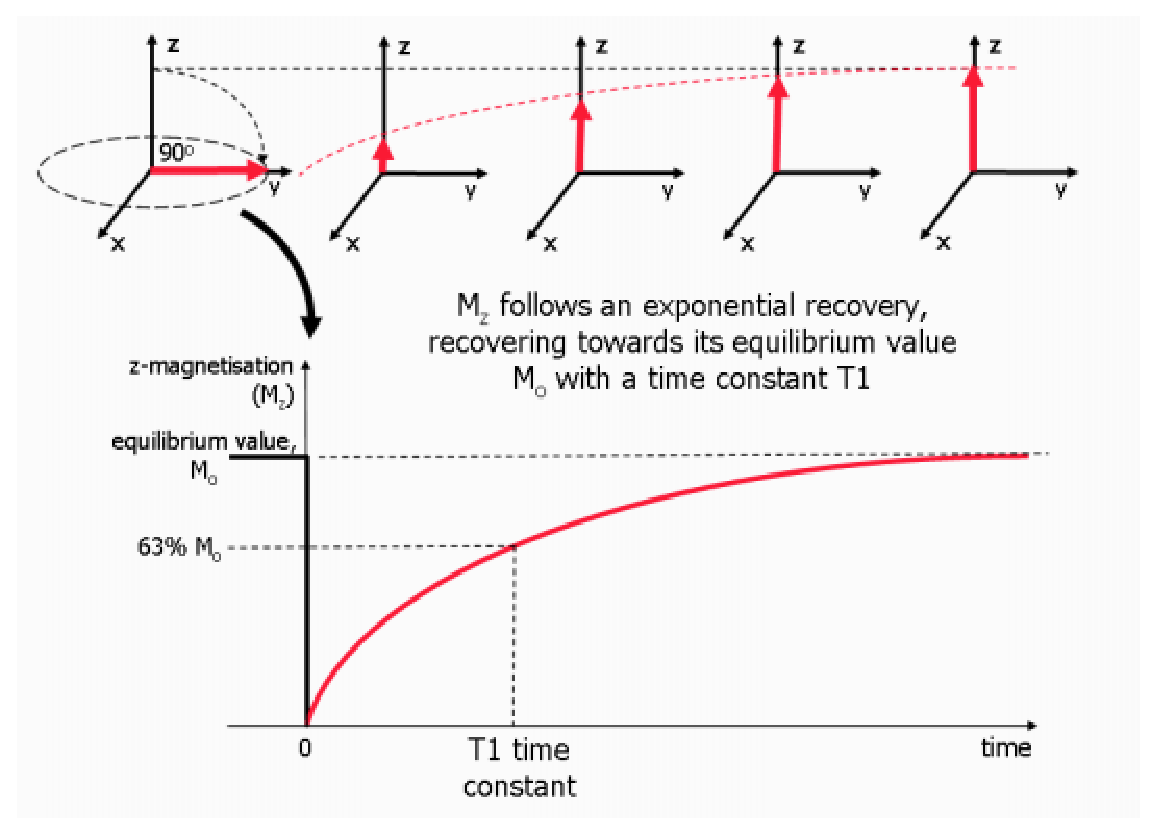
\includegraphics[width=0.7\textwidth]{contraste_T1}
   \caption{Relajación \Tone. Imagen provisional tomada de la tesis de Sasidhar Tandaki. \citep{tadanki2018}}
 \label{fig:T1}
 \end{figg}
\end{figure}



Conforme \M regresa a apuntar al eje $z$, su proyección sobre dicho eje aumenta progresivamente, y ésto es independiente de hacia qué dirección está apuntando. En otras palabras, cuando hablamos de \Tone, solo nos importa su proyección sobre $z$, que denotaremos con \Mz. Designemos a \Mzero como el la magnitud inicial de \M (antes de nuestro pulso de RF, con el sistema de spins intacto). Dada nuestra excitación con 90\degrees, entonces \Mz vale cero justo después de apagar el pulso de RF, y comienza a crecer hasta que \Mz = \Mzero. No puede crecer más que \Mzero, pues no puede haber más spins que con los que comenzamos. La manera en que \Mz crece tiene una forma peculiar: describe una curva exponencial ascendente (Figura \ref{fig:T1}) que se engloba como
\begin{equation}
\label{eq:Tone}
 M(t) = M_0(1 - e^{-\tau/T1})
\end{equation}
donde $\tau$ indica el periodo de tiempo entre pulsos de RF sucesivos. En nuestro ejemplo, solo hemos utilizado un pulso de RF, así que lo ignoraremos por ahora, pero será importante más adelante.  \Tone es el parámetro principal que le da la forma a la curva exponencial. Es el parámetro que hace que suba más rápida o lentamente, y se mide en unidades de tiempo (s). Mientras más corto es \Tone, la curva sube más rápidamente, mientras que valores largos de \Tone harán que la curva ascienda perezosamente. Revisando la Figura \ref{contraste_T1} y despejando la ecuación \ref{eq:Tone},  podemos darle una intuición sencilla a \Tone como ``el tiempo en que tarda en recuperarse el 67\% de \Mzero''. Insistimos: si \Tone es largo, \Mz tarda mucho en ``crecer'' sobre el eje $z$. 

La eficiencia con la que un tejido transfiere a su entorno el exceso de energía depositado en él mediante la RF determina su tasa de relajación longitudinal, por lo que esta relajación se conoce también como spin-matriz o \textit{spin-lattice}. La grasa y la substancia blanca (repleta de lípidos), por ejemplo, son altamente eficientes en esta transferencia de energía, mientras que el agua libre de los ventrículos cerebrales lo hace lentamente (Figura \ref{fig:contraste_T1_tejidos}).

\begin{figure}[htb]
\begin{figg}
   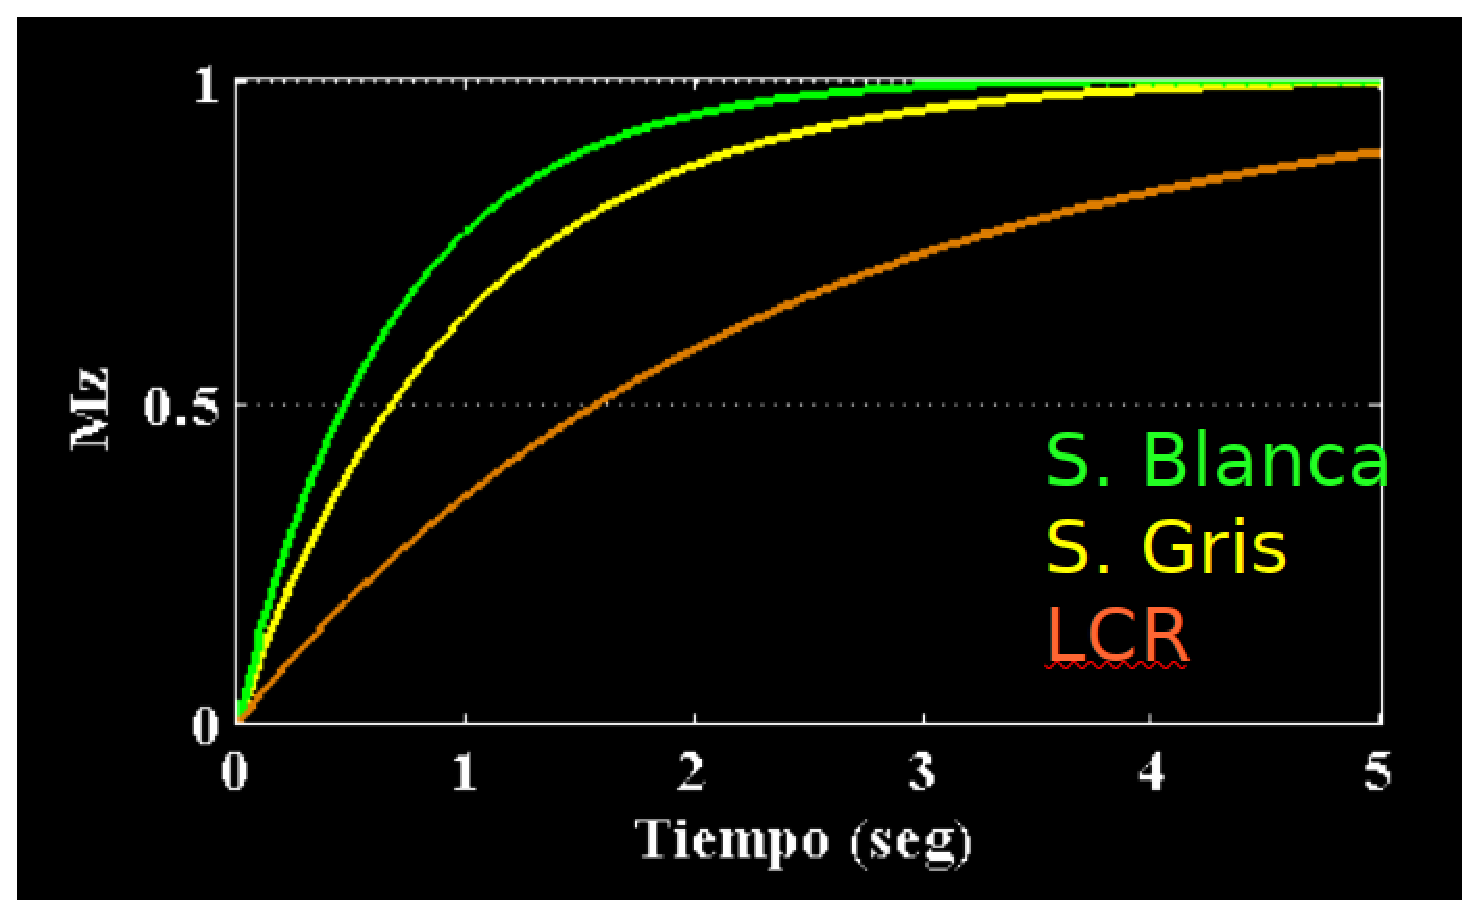
\includegraphics[width=0.7\textwidth]{contraste_T1_tejidos}
   \caption{Diferentes tejidos tienen diferentes tasas de relajación longitudinal \Tone. En el cerebro adulto, la substancia blanca presenta la relajación longitudinal más acelerada; por el contrario, el líquido cerebro-raquídeo (LCR) disipa el exceso de energía lentamente y presenta una relajación longitudinal lenta, con un \Tone largo.}
 \label{fig:contraste_T1_tejidos}
 \end{figg}
\end{figure}


\section{Relajación transversal: \Ttwo}
\index{T2|textbf}
Para poder describir este tipo de relajación, debemos recordar que \M es el vector resultante de la suma de muchas barras magnéticas ($\mu$) asociadas a cada uno de los protones de H (ver Capítulo \ref{chapter_fenomeno}). Cuando estuvo prendido el pulso RF, todos estos pequeños imanes $\mu$ se alinearon con \Bone, es decir, la radiofrecuencia. Si el pulso de RF fue de 90\degrees, todos estarán ahora alineados en algún lugar del plano $x,y$. Todos apuntan al mismo sitio, y si los vemos desde arriba (volteando a ver el plano $x,y$), estarán todos ``apilados''. La suma vectorial de muchos pequeños vectores que apuntan en la misma dirección y sentido resulta en un vector de gran magnitud, con la misma dirección y sentido. Esto es similar a cuando varios niños jalan de una cuerda: aunque cada niño tenga poca fuerza, la suma de todas sus fuerzas será tal que podrían jalar un auto. En un escenario perfecto, \M se relajaría únicamente por la influencia de \Tone, porque todos los spins precesan perfectamente a la misma frecuencia. En el mundo real, en el tejido que estamos analizando, existen pequeñas imperfecciones del campo magnético que experimentan los distintos spins. Consideremos un pixel en un sitio anatómico, por ejemplo el tálamo, en el cerebro. Un pixel tiene dimensiones de alrededor de 1 mm por lado, donde pueden caber muchísimas neuronas, células gilales, capilares sanguíneos, etc. La composición molecular y atómica de todas estas estructuras es variada, y pueden contener elementos que interaccionan con el campo magnético principal \Bzero, por ejemplo el Fe que está en la hemoglobina de la sangre, o el Cu que suele acumular el tálamo a lo largo de la edad. Si nuestro voluntario está en un resonador de 3 teslas, a nivel microscópico existirán pequeñas desviaciones de 3 teslas, haciendo que algunos spins experimenten un poco más de 3 teslas, mientras que otros (en el mismo pixel, pero unos micrómetros más alejados de los primeros) experimenten un poco menos de 3 teslas. 



Recordemos que la frecuencia de precesión \omegazero de los protones de H depende únicamente del campo magnético \Bzero que experimentan. Las variaciones intra-pixel de \Bzero son muy pequeñas (microteslas), pero provocan que cada grupo de spins precese a distintas frecuencias. Las diferencias de frecuencias entre los diferentes spins son muy sutiles, pero reales. Esto va a traducirse que, una vez que el pulso de RF se apague, los spins que precesan más rápido ``se adelanten`` a los que precesan más lento. Con el paso del tiempo, veríamos que los spins que componen a \M comienzan a \textit{desfasarse} entre ellos. Mientras más se desfasen, la suma vectorial de ellos tenderá a cero, y \M irá desapareciendo. Como se revisó en la sección \ref{section:mrsignal}, la señal que obtenemos requiere que \M esté en el plano $x,y$, y si \M va desapareciendo, nuestra señal entonces también.

En el marco de referencia en rotación, el desfasamiento de los spins se observa como un abanico que se abre con respecto al punto en el plano $x,y$ donde cayeron los spins posterior al pulso RF. Es decir, los spins que precesan perfectamente con frecuencia \omegazero se mantienen en ese punto; los que precesan ligeramente más rápido (y se adelantan) se van alejando (por ejemplo, a favor de las manecillas del reloj), mientras que los que precesan lentamente (se retrasan) se mueven en el otro sentido (en contra de las manecillas del reloj). La suma vectorial de todos esos spins irá disminuyendo a lo largo del tiempo, con lo que la señal irá decayendo.


La curva que describe la señal a lo largo del tiempo es exponencial, pero en este caso decreciente (Figura \ref{fig:T2}), y descrita como:

\begin{equation}
\label{eq:T2}
 M_{xy}(t) = M_{xy,max} (e^{-t/T2})
\end{equation}

donde $M_{xy,max}$ es la magnitud del componente de \M que se encuentra en el plano $x,y$ justo después de la excitación (la cantidad máxima de señal que podemos obtener tras la excitación y, en el caso de una desviación de 90\degrees, sería igual a \M). En el exponente vemos a $T_2$, que está dictando la forma de la curva exponencial, y se mide en unidades de tiempo (s). Si \Ttwo es largo, entonces la señal se pierde lentamente; si es corto, en poco tiempo habremos perdido nuestra señal. Intuitivamente, \Ttwo es el tiempo al cual solamente queda el 37\% de la señal \Mxy original. Finalmente, $t$ indica en qué momento estamos valorando cuánta señal hay, y será un parámetro que podremos explotar más adelante para extraer más o menos contraste tipo \Ttwo. 

\begin{figure}[htb]
\begin{figg}
   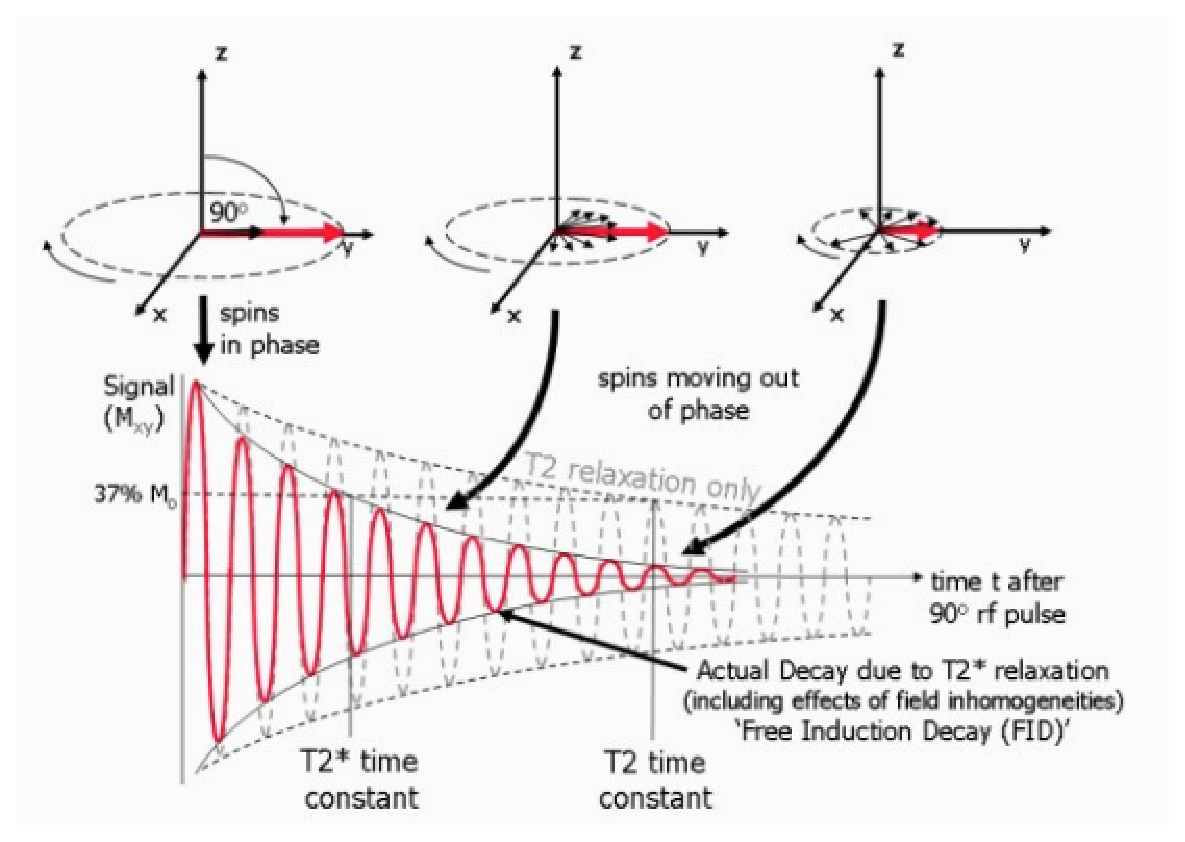
\includegraphics[width=0.7\textwidth]{contraste_T2}
   \caption{Relajación \Ttwo. Imagen provisional tomada de la tesis de Sasidhar Tandaki. \citep{tadanki2018}}
 \label{fig:T2}
 \end{figg}
\end{figure}


Existen dos tipos de desfasamientos producidos por inhomogeneidades de \Bzero: las reversibles y las irreversibles. El desfasamiento producido por las inhomogeneidades irreversibles se conoce com \Ttwostar (pronunciado \Ttwo estrella) \index{T2*|textbf}. Este desfasamiento reversible se suma al desfasamiento intrínseco del tejido, por lo que podemos considerar a \Ttwostar como la relajación \textit{observada} o efectiva, mientras que el \Ttwo es la relajación \textit{real}. La relación entre \Ttwo y \Ttwostar es

\begin{equation}
 1/T2^* = 1/T2 + 1/T2'
\end{equation}
donde $1/T2'= \Delta B_i$, es decir, las inhomogeneidades de \Bzero a lo largo de un voxel \footnote{http://mriquestions.com/t2-vs-t2.html}. Por lo tanto, \Ttwostar es \textit{siempre} más corto que \Ttwo.


Dada la variedad de composiciones tisulares, cada tejido tiene un \Ttwo (y \Ttwostar) particular, por lo que las curvas asociadas a cada uno de ellos son distintas (\figurapendiente). Tejidos altamente heterogéneos, o en cuyo interior existan elementos que provocan inhomogeneidades microscópicas de \Bzero, tendrán \Ttwo corto.

\section{Ecos}
\index{eco|textbf}
En la ecuación \ref{eq:T2} vimos que la señal obtenida es distinta dependiendo de en qué momento $t$ la evaluamos. Pero, ¿Cómo controlamos $t$? A través de la generación de un \textit{eco}, quizás uno de los trucos más asombrosos de la resonancia magnética, desarrollado por Erwin Hahn en la década de los 1950 y que debió haberle valido el premio Nobel \citep{mansfield2013long}. Igual que el eco de un grito emitido frente a una barranca, el eco de Hahn tiene como objetivo recuperar una señal que parecía perdida para siempre (en este caso, el FID). Siguiendo con las similitudes entre los ecos, es posible recibir un tren de ecos, cuyas magnitudes van decreciendo progresivamente ({\Large ¡Eco!} {\normalsize ¡Eco!} {\small ¡Eco!} {\tiny ¡Eco!}). Existen dos tipos de eco, que dependen de la manera en que se generan: eco de gradiente, y eco de spin. Para cada uno de ellos, el operador puede decidir en qué momento se formará el eco.

\subsection{Eco de gradiente}
\index{eco de gradiente|textbf}
Dado que la frecuencia de precesión de un spin depende únicamente del campo magnético que experimenta, podemos hacer que un grupo de spins con localizaciones espaciales distintas precesen a diferentes frecuencias. Para ello, modulamos linealmente el campo magnético \Bzero, haciéndolo más potente de un lado, y menos potente del otro. Esto es también el pilar de la codificación espacial (Capítulo \ref{chapter_espacial}), pero por ahora lo usaremos para generar un eco de gradiente .\footnote{En resonancia hay varios trucos, y la mayoría se pueden usar en distintos escenarios para obtener distintos resultados, pero deben usarse en momentos específicos y no simultáneamente. Por ejemplo, un gradiente de campo magnético puede usarse primero para producir un eco de gradiente, y más adelante para realizar codificación espacial.} En presencia de un gradiente de campo magnético, los spins que se encuentran en un pixel presentarán una gama de frecuencias de precesión, lo que provocará que se desfasen fácilmente. Es más fácil imaginar ésto en el campo de referencia en rotación, donde el desfasamiento se asemeja a un abanico que se abre. En el caso del eco de gradiente, el desfasamiento fue controlado por el operador y es fácil de revertir mediante la inversión del gradiente. El lugar en el espacio donde antes había un campo magnético más potente es ahora más débil, y viceversa. La amplitud y dirección del gradiente del campo magnético debe ser invertida a la perfección para lograr un eco de gradiente (el segundo gradiente es un espejo del primero). Durante la presencia del primer gradiente, los spins se desfasan, y los que experimentan más campo magnético precesan más rápidamente y se adelantan a los lentos; al invertir el gradiente los spins que precesaban lento ahora lo hacen rápido y alcanzan a los ahora lentos (se refasan; el abanico se cierra). Durante el primer gradiente, la suma vectorial que genera la señal va tendiendo a cero, pero durante el segundo gradiente su magnitud crece nuevamente, acercándose (pero no alcanzando) a su magnitud original. Así, la señal que se hubiera perdido como un FID se recupera como un eco. Puede incluso repetirse la inversión del gradiente, obteniendo ecos sucesivos, aunque éstos serán cada vez de menor magnitud. El operador decide cuándo se forma el eco al decidir el momento en que se prende el gradiente que desfasa los spins, y la duración del mismo (que será idéntica en el gradiente inverso). El periodo de tiempo que transcurre entre el pulso de RF excitador y la obtención de la señal máxima del eco se conoce como \textit{Tiempo de Eco} (TE) \index{TE}. Un TE puede ser corto si se desarrollan los gradientes poco tiempo después del pulso de RF, y puede ser largo si el operador se espera mucho tiempo después del pulso RF para usar los gradientes. Obviamente, si el TE es demasiado largo, el desfasamiento no reversible entre los spins habrá dominado, y no podremos lograr un eco.

Una analogía muy útil (y utilizada en casi todos los libros de texto) es la de la competencia de atletismo que debemos aclarar sucede en el marco de referencia en rotación. Imaginemos una carrera de 400 m libres, donde todos los corredores inician en el mismo punto (están en fase), siendo el equivalente al momento inmediatamente posterior al apagar el pulso de RF. Los corredores arrancan; los más veloces toman la delantera, y los más lentos van quedando atrás (se desfasan entre ellos). Al cabo de un tiempo determinado, un réferi indica con un silbato que ahora todos deben correr en sentido contrario (la orden es: ``media vuelta, ¡ya!''), con lo que su carrera se dirige ahora justo al punto donde iniciaron. Como los corredores lentos habían quedado atrás, les resulta más cerca la nueva meta, mientras que los corredores veloces están lejos; como sus velocidades de ida y de vuelta son similares, los corredores veloces alcanzan a los lentos y todos llegan a la nueva menta de manera casi simultánea (en fase). Recordemos que mientras exista mucha coherencia de fase, la señal será mayor, con lo que podemos reforzar que al inicio de la carrera había mucha señal, que decayó rápidamente en función del desfasamiento entre corredores, pero que se recuperó al momento de sincronizarse de nuevo sus fases después de la inversión de su sentido al correr.


Los ecos de gradiente son capaces de recuperar un eco y son sensibles a los fenómenos relativos a \Ttwostar. Es decir, son capaces de recuperar la señal perdida por inhomogeneidades reversibles. Entre otras aplicaciones, los ecos de gradiente son de gran utilidad en la clínica para evaluar hemorragias, malformaciones arterio-venosas, y en la investigación son la piedra angular de la resonancia magnética funcional (Capítulo \ref{chapter_bold}), que es sensible al nivel de oxigenación de la hemoglobina (nótese como estos ejemplos comparten su dependencia con la sangre, y el \ce{^{26}Fe} en ella).

El operador puede decidir cuándo ejercer los gradientes de campo magnético, así como su duración. Esto determinará el momento en que se generará el eco, y por lo tanto, es utilizado para controlar la cantidad de contraste \Ttwostar presente en la imagen (ver sección \ref{sec:mod_contraste}).


\subsection{Eco de spin}
\index{eco de spin|textbf}
Los ecos de spin son capaces de recuperar mucho más señal que los ecos de gradiente, y son sensibles a procesos referentes a \Ttwo. Después del pulso de RF que desvía a \M, el eco se produce mediante un pulso de RF que voltea a \M 180\degrees. En el marco de referencia en rotación, después del pulso de RF, comienza el desfasamiento (gobernado por \Ttwo). Despueś de cierto tiempo, se presenta un pulso de RF de 180\degrees, que invierte la posición de los spins sin alterar el sentido en el que se desfasan. Al hacerlo, provoca que los spins vuelvan a estar en fase. 

Necesitaremos echar mano nuevamente de nuestra imaginación para aclarar el eco de spin, utilizando la analogía de la carrera de atletismo que usamos para explicar el eco de spin, pero con ciertas modificaciones fantásticas. En este caso, la pista de atletismo está en el espacio exterior, y los corredores usan zapatos especiales que les permiten permanecer adheridos a ella. La carrera comienza con todos los atletas en el mismo punto (en fase, justo después del pulso RF), y comienzan su recorrido, presentando un desfasamiento entre ellos en función de las distintas velocidades de cada corredor. Ahora, en vez de la orden de correr en sentido inverso (como sucedió en el eco de spin), toda la pista sufre una inversión de 180\degrees. Los corredores parecen ahora correr en la cara inferior de la pista, de la que afortunadamente no caen, gracias a sus zapatos especiales; ellos continúan su carrera, sin darse cuenta del suceso, y sin cambiar su ritmo de avance. Para un espectador será evidente que los corredores lograrán recuperar la homogeneidad de fase, en el lado extremo de la pista de atletismo. Si la carrera continúa, volverán a desfasarse, y podrá repetirse el fantástico suceso de voltear la pista para ponerlos de vuelta en fase en repetidas ocasiones. Los ecos sucesivos así formados serán cada vez de menor magnitud, pues cada vez será más dificil que se recupere la totalidad de la fase entre corredores (spins), y después de un número no muy grande de ecos de spin, la señal habrá desaparecido, debido al desfasamiento irreversible propio de cada tejido.

Al igual que en el eco de gradiente, el \textit{Tiempo de Eco} (TE) \index{TE} es el periodo de tiempo que transcurre entre el pulso de RF excitador y la obtención de la señal máxima del eco. El operador decide cuándo sucede el eco al determinar el periodo de tiempo que transcurre entre el pulso excitador de RF, y la aplicación del pulso de RF de 180\degrees usado para reenfocar los spins. De esta manera, el pulso de 180\degrees sucede en $t=TE/2$. 



\section{Control del contraste}
El contraste es la diferencia de la intensidad de señal entre tejidos, y para fines prácticos la consideraremos como la diferencia de intensidad entre pixeles, en el supuesto de que distintos pixeles están ocupados por tejidos de composiciones distintas. Por ahora tendremos que ignorar cómo se realiza la codificación espacial (ver Capítulo \ref{chapter_espacial}), pero las descripciones que haremos se estarán llevando a cabo simultáneamente en todos los pixeles de la imagen. El concepto de contraste es fundamental, pues en las imágenes de resonancia magnética la intensidad de cada pixel está en unidades arbitrarias, y lo que importa es qué tan distintas son las intensidades entre pixeles.

En resonancia magnética existen múltiples mecanismos de contraste, lo que hace a la técnica muy versátil. Compárese con otros métodos de imagen, como la tomografía por rayos X, cuyo único mecanismo generador de contraste es la absorbancia de la radiación. Entre todos los mecanismos de contraste, los más importantes y siempre presentes son los relacionados a los fenómenos de relajación arriba descritos. El otro generador de contraste omnipresente es la cantidad de H en el tejido, que se conoce como \textit{densidad de protones} (el nivel de hidratación de un tejido). 

Al momento de adquirir imágenes de resonancia magnética, el operador puede decidir qué tanto influye uno u otro mecanismo generador de contraste. A las imágenes obtenidas se les suele llamar por el tipo de contraste que predomina. Por ejemplo, si el fenómeno de relajación longitudinal es el mayor generador de contraste, tendremos una imagen ``pesada'' o ``ponderada'' a \Tone (en inglés, \Tone-weighted). Para que un tipo de contraste predomine, habrá que minimizar la contribución de los otros. El único tipo de contraste que evidentemente no podremos controlar sin hacer daño al tejido (¡y participante!) es densidad de protones.

\subsection{Modulación de contraste \Ttwo}
\label{sec:mod_contraste}
Para maximizar la contribución de \Ttwo, debemos adquirir nuestra imagen justo cuando exista mayor diferencia entre las magnitudes de las señales de los diferentes tejidos (el $t$ de la ecuación \ref{eq:T2} que provea magnitudes disímiles). Si $t$ es muy corto, tendremos a todas nuestras señales con valores cercanos al máximo (a la izquierda en la Figura \ref{fig:contraste_T1_tejidos}). Si $t$ es demasiado largo, hemos perdido la señal de todos los tejidos por igual (hasta la derecha en la misma figura). Pero con $t$ medianamente largo, algunos tejidos brindarán mucha señal, mientras que otros brindarán poca, impartiendo contraste tipo \Ttwo. Contrariamente, para minimizar la contribución de \Ttwo debemos obtener nuestra señal en $t$ muy corto, de manera que todos los tejidos brinden el máximo de señal posible, con diferencias entre ellos dictaminadas únicamente por su densidad de protones. Como se detalla en la página \pageref{sec:imagenescomunes} y el Capítulo \ref{chapter_secuencias}, $t$ se controla mediante el tiempo de eco, TE. \index{TE}

\subsection{Modulación de contraste \Tone}
Entender la contribución de \Ttwo es relativamente sencillo, pues el fenómeno sucede en el plano $x,y$, que es de donde podemos captar señal. Pero \Tone sucede en el eje $z$, invisible para resonancia, lo que nos puede confundir. Para poder inyectar contraste tipo \Tone, no podemos hacer solo un experimento, debemos hacer varios. La rapidez con la que repitamos nuestros experimentos serán determinantes para que \Mz se vea modulada, y por tanto la señal que podemos poner en el plano $x,y$ mediante pulsos excitadores. En la ecuación \ref{eq:Tone} el parámetro $\tau$ indica qué tan rápido hacemos pulsos excitadores sucesivos, y comúnmente se le conoce como \textit{Tiempo de Repetición}, o TR (detallado en Capítulo \ref{chapter_secuencias}) \index{TR (Tiempo de repetición)|textbf}. Imaginemos, pues, que iniciamos nuestro experimento, y llamaremos a \Mz original como \Mzero. Tras un pulso que desvíe 90\degrees, \Mz partirá de cero e incrementará exponencialmente, y si lo dejamos mucho tiempo ($\tau\xrightarrow{}\infty$), crecerá tanto como \Mzero. Pero, si antes de que \Mz llegue a valer \Mzero aplicamos un nuevo pulso de RF, estaremos excitando únicamente la porción de \Mz que ya se había relajado, y la señal que obtendremos será entonces menor que la que hubiéramos obtenido con tan solo el primer pulso de RF. Hemos visto en el plano $x,y$ la consecuencia de no haber permitido la completa relajación longitudinal. El caso extremo de esta acción sería hacer un TR exageradamente corto. En este escenario, comenzaríamos con \Mz = \Mzero, tendríamos un primero pulso excitador (90\degrees, en este ejemplo), que llevaría a \Mz a un valor de cero; antes de recuperarse \Mz se recibiría un nuevo pulso excitador, y después otro, y así sucesivamente. El resultado sería que \Mz sería esencialmente obliterada y consecuentenemente no habría posibilidad de recibir señal (no se puede colocar a \M en el plano $x,y$ si no hay nada en \Mz). 

Hagamos una burda analogía para comprender cómo influye TR en el contraste \Tone. Recordemos el juego \textit{Whack-a-mole}, disponible en algunos restaurantes infantiles (Figura \ref{fig:whack}). En este juego, el objetivo es golpear con un mazo unos topos que salen de sus guaridas subterránas, asomando su cabeza. Algunos topos asoman su cabeza velozmente, mientras que otros son más lentos en su ascenso. Nos daremos una ventaja competitiva: en vez de usar un mazo y golpear individualmente a los topos, usaremos una tabla que los hundirá a todos simultáneamente. En este escenario imaginario, además, jugaremos a colectar a los topos (o fragmentos de ellos) en una canasta colocada a un costado del tablero. Para ello, un jugador utilizará un bat (o un temible machete) para guadañar a los topillos que se hayan aventurado a la superficie, lanzándolos hacia la canasta. La condición en este ejercicio (mental, afortunadamente), es que cada madriguera determina la velocidad de ascenso del topillo en cuestión, y el color de su camiseta (porque una vez que llegue a la canasta necesitamos saber de qué madriguera provino). Podemos determinar la frecuencia con la que damos un tablazo. Si lo hacemos exageradamente rápido, no permitiremos que ningún topillo asome su cabeza, y no recibiremos nada en la canasta (nuestro sádico amigo estará haciendo \textit{strikes} a cada intento entre tablazos). Si, por el contrario, tardamos mucho tiempo entre tablazos, todos los topillos con camisetas de distinto color estarán equitativamente representados en la canasta del horror. Pero existirá un punto intermedio en el ritmo de los tablazos, de manera que los topillos con ascenso rápido llegarán completos a la canasta, recolectaremos fragmentos de aquéllos con ascenso intermedio, y los demasiado veloces no estarán muy representados. En esta analogía, el ritmo de los tablazos es el TR, la velocidad de ascenso de los topillos es el \Tone del tejido, y el color de los topillos es la codificación espacial (Capítulo \ref{chapter_espacial}). Podemos ver nuevamente que la excitación repetida modula la magnitud de \Mz y por ende la señal potencial recibida.


\begin{figure}[htb]
\begin{figg}
   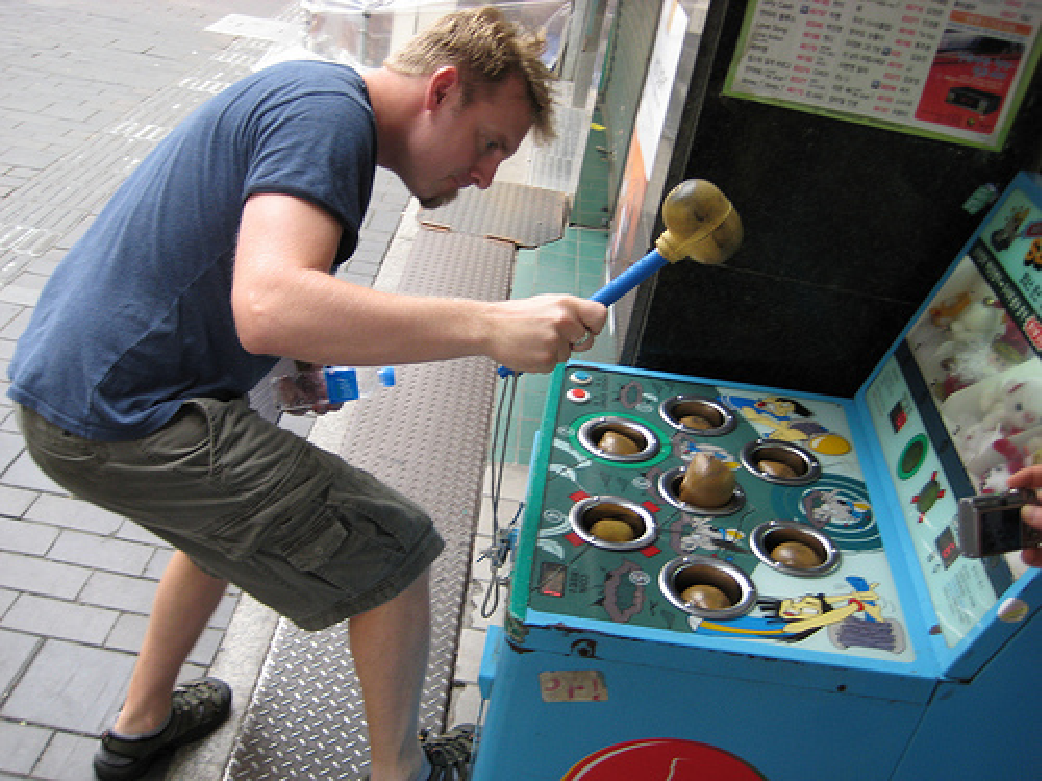
\includegraphics[width=0.7\textwidth]{whack}
   \caption{Juego de \textit{Whack-a-mole}.}
 \label{fig:whack}
 \end{figg}
\end{figure}


\subsection{Los tres tipos de imágenes más comunes}
\label{sec:imagenescomunes}
Sabiendo modular la contribución del contraste \Tone y \Ttwo, y admitiendo que nada podemos hacer por la densidad de protones en un tejido, tenemos oportunidad de generar cuatro diferentes imágenes (Figura \ref{fig:diferentes_contrastes}). De ellas, solo tres de ellas son de utilidad clínica, pues es difícil interpretar una imagen pesada simultáneamente a los tres mecanismos de contraste.


\subsubsection{Imagen pesada a \Tone}
Para hacer una imagen con este contraste, debemos maximizar la contribución de la relajación longitudinal, a la vez que minimizamos la contribución de la relajación transversal. Debemos, entonces, utilizar un TR tal que no sature la señal (no demasiado corto, recordemos a los topillos), ni tan largo que permita la relajación total de todos los tejidos. Le llamaremos un TR corto, entendiendo largo en el contexto del \Tone propio del tejido. Por ejemplo, para tejidos con valores \Tone en el rango de [400 1500] s, un TR largo sería alrededor de esos mismos valores, o incluso menor.

Para minimizar la contribución de \Ttwo, usaremos un TE corto. De esta forma, estaremos adquiriendo nuestra señal antes de que se exprese un desfasamiento diferencial entre tejidos (los valores de los diferentes tejidos son muy similares entre ellos en la parte más izquierda de la \figurapendiente. Uno puede pensar que también son muy similares entre ellos en la parte más a la derecha de la misma figura, y tendría razón en cuanto a las mínimas diferencias entre ellos, pero tendríamos muy poca o nula señal, con lo que nuestra imagen sería inútil.

Maximizando entonces la contribución de \Tone mediante un TR corto, y minimizando la contribución de \Ttwo con un TE corto, obtendremos una imagen pesada a \Tone. La substancia blanca, teniendo el \Tone más corto, logra brindar mucha señal y es brillante, mientras que el líquido-cefalo-raquídeo presenta el patrón inverso, con la substancia gris con intensidad intermedia.

\subsubsection{Imagen pesada a \Ttwo}
Ahora debemos hacer el ejercicio inverso al anterior. Minimizaremos la contribución de \Tone dejando que todos los tejidos se relajen totalmente, lo que podremos lograr dándoles suficiente tiempo para que el fenómeno de relajación suceda, con un TR largo. Nuevamente, entendemos largo en el contexto del \Tone de los tejidos de interés, y un TR largo es habitualmente unas dos o tres veces más largo que el \Tone más largo (formalmente deberíamos esperar una eternidad TR $\xrightarrow{}\infty$, pero nadie tiene tiempo para ello).

Para maximizar la influencia de la relajación transversal, dejaremos que ésta suceda con un TE largo. Un TE muy corto, como vimos, no permite la diferenciación de las intensidades de señal entre tejidos. Un TE largo ronda o excede un poco los valores de \Ttwo de los tejidos, pero no va más allá de tres veces dicho valor, porque para entonces todos los tejidos ya tendrán totalmente desfasados sus spins, y no podrán darnos nada de señal. Los tejidos que se relajan lentamente, como el líquido cerebro-raquídeo, brindarán mucha señal, mientras que los que se relajan rápido, como la substancia gris, serán más obscuros.

\subsubsection{Imagen pesada a densidad de protones}
Siendo la densidad de protones el único mecanismo de contraste que no podemos modular con ningún parámetro, la estrategia será minimizar la influencia de los otros dos mecanismos de contraste, \Tone y \Ttwo. Repasando la información que acabamos de revisar, sabemos que podemos minimizar la contribución de \Tone con un TR largo (todos los tejidos se relajarán totalmente), mientras que un TE corto minimizará la contribución de \Ttwo (los spins de todos los tejidos están aún todos en fase). Por lo tanto, la diferencia en la intensidad entre los diferentes tejidos estará dictada primordialmente por sus diferentes niveles de hidratación. El agua del líquido cerebro-raquídeo será muy brillante, mientras que el hueso del cráneo será el tejido más obscuro en una imagen de cerebro.



\begin{figure}[htb]
\begin{figg}
   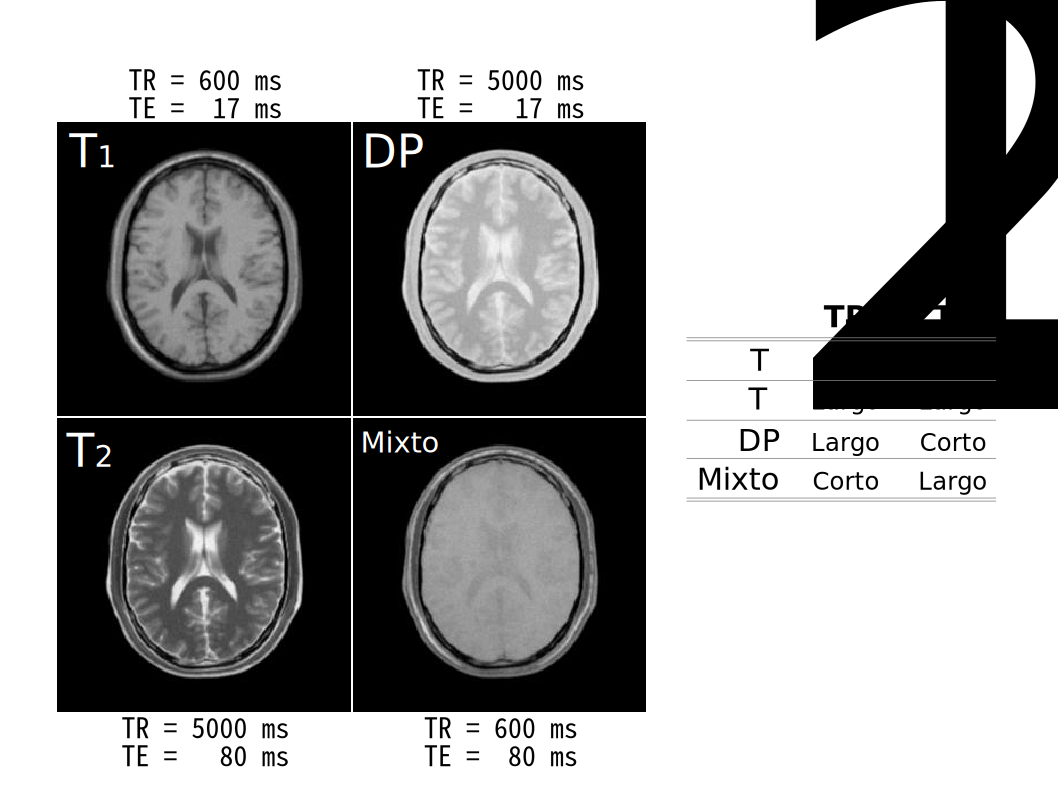
\includegraphics[width=0.7\textwidth]{diferentes_contrastes}
   \caption{Imágenes pesadas a diferentes contrastes obtenidas en un resonador de 3 teslas. Para cada imagen se indica el mecanismo de contraste que predomina; por ejemplo la imagen pesada a \Tone está indicada como \Tone. Adyacente a cada imagen se indican los parámetros TR y TE correspondientes. La tabla de la derecha resume en términos cualitativos los valores TR y TE para obtener cada tipo de imagen. La imagen con contraste mixto es difícil de interpretar y de poca utilidad. TR: tiempo de repetición; TE: tiempo de eco; DP: densidad de protones.}
 \label{fig:diferentes_contrastes}
 \end{figg}
\end{figure}



% Como se mencionó en el capítulo anterior, cuando se aplica un campo magnético externo o Radiofrecuencia (\Bone) superior al campo magnético principal (\Bzero),  nuestros spins o protones de hidrógeno comienzan a precesar en dirección a este nuevo campo magnético.
% 
% ¿ Pero que ocurre cuando este campo magnético externo  se “apaga”?
% 
% Es lógico pensar que los spins regresarán a B0 (su posición original sobre el eje \textit{z}),  pero es la trayectoria que realizan la que es de interés para la obtención de una Imagen de Resonancia Magnética. A este fenómeno se le conoce como Relajación y es el proceso que llevan a cabo los spins para regresar a su sitio de origen en este caso R0 también conocido como \Mz, mismo que logran liberando energía en su trayectoria. 
% 
% La relajación ocurre debido a que los spins desprenden la energía que habían absorbido al entrar en resonancia.
% 
% 
% En la Relajación de estos spins ocurren dos fenómenos simultáneamente, el primero llamado relajación longitudinal o \Tone y el segundo conocido como relajación transversal o \Ttwo. 
% 
% \section{RELAJACIÓN LONGITUDINAL (\Tone)}
% 
% Llamada de esta forma porque es el fenómeno que ocurre sobre el eje \textit{z}, es una constante en el tiempo de la trayectoria del spin, para retomar su lugar sobre \Mzero.
% Se define como: ``El tiempo que tarda en recuperarse el 63\% del \Mz original''
% 
% 
% Tras  el pulso de radiofrecuencia nuestro spin cambió su eje magnético al plano de las \textit{x}. Esta es la razón que provoca  que parezca pequeño sobre el eje \textit{z}.
% 
% Una vez que el pulso de radiofrecuencia se elimina, el spin retomará su dirección. Comienza entonces a precesar más lentamente y a regresar a \Mz por lo que este comienza a crecer conforme los segundos transcurren (\Tone). Finalmente el protón de Hidrógeno regresa a su posición original provocado por el campo magnético principal (\Mz).
% 
% 
% El fenómeno de relajación T1 se define como:
% ``El tiempo que tarda el spin en recuperar su campo magnético original (\Mz) en un 63\%''
% 
% En la representación gráfica se observa como una exponencial ascendente.
% 
% 
% 
% \section{RELAJACIÓN TRANSVERSAL (\Ttwo)}
% 
% Al igual que el concepto antes descrito, el nombre es mera cuestión de lógica, se le denomina Relajación Trasversal por que ocurre sobre el plano \textit{x,y}. Otra forma en la que se conoce al \Ttwo es como Relajación Spin- Spin o \Ttwop ya que el fenómeno se observa en un conjunto de protones de hidrógeno. En el caso de la relajación \Ttwop  la representación gráfica nos habla de una caída en la señal original por lo que se define de la siguiente forma:
% ``Tiempo en el cual solamente queda el 37\%de la señal \Mxy original, es decir de la emitida por el pulso de radiofrecuencia''
% 
% 
% 
% Comencemos por entender que el T2 es el resultado de la actividad de varios spins. En un inicio como se ha venido mencionando la Radiofrecuencia (\Mzero) que provocó que nuestros spins cambiaran del eje \textit{z} al plano \textit{x,y}, también provocó que varios spins precesaran al mismo tiempo, es decir todos giraban a la misma frecuencia. 
% 
% 
% Al suspender \Mzero, cada spin comienza a relajarse a su propio tiempo , y poco a poco cada uno regresa a su \Mzero, esto provoca que se desfasen uno del otro.
% 
% 
% \subsection{Fenómeno \Ttwostar}
% 
% El desfase es provocado por inhomogeneidades en el campo magnético que experimentan los protones de hidrógeno y debido a que ocurren en el fenómeno \Ttwo se les conoce como \Ttwostar, estas inconsistencias pueden ser de dos tipos dependiendo de que las genere:
% 
% \begin{description}
%  \item [Intrínsecas]  Suceden por acumulación de metales en el paciente.
%  \item [Extrínsecas]  Se deben a inhomogeneidades en el campo magnético del resonador,  presencia de objetos metálicos, e incluso productos para el cabello.
% \end{description}
% 
% 
% 
% 
% \section{Contraste}
% 
% 
% El contraste se define como: ``la diferencia entre la intensidad de señal entre dos muestras, secundario a las propiedades magnéticas de las mismas''.
% 
% Tras el pulso de radiofrecuencia inicial, la energía que se libera de nuestro Spin en los fenómenos de \Tone y \Ttwo (\Ttwop - \Ttwostar),  es captada por una antena que codifica la señal en nuestro aparato de resonancia magnética, y que se puede observar como una ``disminución en la señal'' es decir un decremento de nuestro pulso inicial hasta el regreso a su estado basal, a esta caída se le conoce como Free Induction Decay (FID).
% 
% 
% 
% La antena que capta la señal de radiofrecuencia, lo hace simultáneamente para todos los spins que se le diga que debe captar señal, por lo que al revisar esta señal ``cruda'' tendremos entremezclado la señal de todos nuestros spins, posteriormente estas señales podrán ser diferenciadas mediante un análisis de Fourier. 
% 
% 
% 
% Algo que debemos tomar en cuenta es que este proceso está sucediendo en los tejidos y que la conformación de estos es muy diferente; ya sea que hablamos de sangre, grasa, hueso etc. Debido a lo diverso de la composición de las estructuras que rodean a nuestro protón, la liberación de esta energía y el retorno a su campo magnético original (\Mz) será distinta para cada protón al igual que la señal que captaremos con nuestra antena.
% 
% El análisis de estas señales es lo que nos permitirá diferenciar estructuras dependiendo si al ``leer'' estas señales lo hacemos más influenciados por el fenómeno \Tone o \Ttwo, a esto se le denomina de forma genérica \textit{potenciar} se dice que nuestra imagen esta potenciada a uno de estos fenómenos de resonancia magnética según lo observado en nuestra imagen final , es justo este proceso el que nos permite crear el contraste de las estructuras aprovechando su comportamiento bajo resonancia magnética.
% 
% 
% \subsection{Imágenes potenciadas a densidad de protones}
% 
% Como se ha venido mencionando, la magnetización de nuestros spins está influenciada por la densidad de los mismos en la muestra que se esté estudiando. De ahí que podamos jugar con la manera en la que observamos estas imágenes, y para el caso de las imágenes potenciadas en densidad se sigue la siguiente regla:
% 
% ``La intensidad de la imagen es directamente proporcional a la densidad de protones de hidrógeno''
% 
% ¿Qué quiere decir esto? que al hacer la lectura de nuestra imagen el lugar donde se reciba más señal será donde existan más protones de hidrógeno. Se sabe que los tejidos tienen distintas densidades, dependiendo si son grasa, hueso, LCR, etc.
% 
% 
% Estas imágenes se obtienen al enviar un pulso de radiofrecuencia (RF) de 90º  y esperando un tiempo largo (tiempo de repetición o TR) antes de dar nuestro siguiente pulso, para permitir que los tejidos envíen la señal de sus spins.
% 
% 
% \subsection{Imágenes potenciadas a \Tone}
% 
% Cuando hablamos de imágenes potenciadas a \Tone nos referimos a que al momento de codificar nuestra imagen lo hicimos tomando en cuenta las propiedades de la relajación longitudinal (\Tone) de nuestros spins y que se ha trabajado bajo la siguiente premisa:
% 
% ``Mientras más rápido libere energía nuestro spin, más rápido regresará a \Mz  y mayor será la intensidad de nuestra señal''
% 
% Un ejemplo de ello es la grasa la cual  se relaja fácilmente ya que su densidad de hidrógenos no es tan alta por lo que su señal es captada más rápido lo que se traduce en mayor señal o contraste blanco.
% 
% 
% Para obtener imágenes potenciadas a \Tone se da un solo pulso de radiofrecuencia de 90\degrees y se realiza la lectura una vez que los spins hayan vuelto a su eje magnético principal.
% 
% 
% \subsection{Imágenes potenciadas a \Ttwo y \Ttwostar}
% 
% Para el caso de las imágenes potenciadas a \Ttwo y \Ttwostar la señal la conseguimos cuando nuestros spins se encuentran sobre el plano \textit{x,y}, captando la señal por medio de nuestra antena. 
% 
% Para que la señal sea más duradera nosotros damos el primer pulso de radiofrecuencia para llevar a todos nuestros spins a \Mx  y antes de que regresen a su campo magnético original , se les aplica otro pulso de 180\degrees  el cual provoca que nuevamente se encuentren y vuelvan a refasarse.
% 
% 
% 
% 




\chapter{Codificación espacial}
\chapterprecis{\noindent \noindent Luis Concha\\Instituto de Neurobiología\\UNAM, Campus Juriquilla}
\label{chapter_espacial}

Si bien el fenómeno de resonancia magnética ha sido explotado durante más tiempo en el área de Química, particularmente mediante la espectroscopía (Capítulo \ref{chapter_espectro}), sin lugar a dudas fue la capacidad de realizar imagen la que revolucionó el campo de la Medicina, tanto en términos clínicos como en el área de investigación. Los métodos para producir imagen mediante el fenómeno de resonancia se gestaron de manera simultánea a la tomografía axial computarizada (TAC, ver Capítulo \ref{chapter_historia}) pero, aunque ambas técnicas comparten muchos conceptos, la manera en que se codifica la posición espacial en resonancia es bastante distinta a como lo hace la TAC, siendo la segunda más intuitiva por ser una simple retro-proyección o transformación de Funk-Radon. Las imágenes de resonancia magnética se obtienen mediante un proceso no necesariamente más complejo, pero sí menos amigable de primera instancia. 

Primero debemos considerar qué es lo que buscamos codificar. En términos prácticos, deseamos saber la relación espacial que guardan con el resonador y con nuestro paciente o muestra, las diferentes partes que lo componen, además de que explotemos los mecanismos de generación de contraste para distinguir entre ellos (Capítulo \ref{chapter_relajacion}). Como en todas las imágenes digitales, tendremos que dividir artificialmente nuestro objeto real (paciente o muestra) en un cierto número de elementos, cada uno denominado \index{pixel} \emph{pixel} (portmanteau de \emph{pic}ture-\emph{el}ement). En el caso que nos compete, buscamos mapear en dos dimensiones (imagen) algo que habita en un espacio tridimensional (paciente u objeto), por lo que cambiaremos el término pixel por \index{voxel} \emph{voxel} (\emph{vol}ume-\emph{el}ement). Es común, aunque no deseable, intercambiar ambos términos, siendo el preferido el término de voxel. Un voxel tiene entonces unas coordenadas y dimensiones en los ejes \textit{x}, \textit{y} y \textit{z}. Es una pequeña caja que contiene tejido, y por lo tanto, muchos átomos de hidrógeno; podemos imaginar cada voxel como tubos de ensaye con muestras, sobre las cuales queremos indagar parámetros claros, como la cantidad de H que contiene. Los métodos que se explican adelante están orientados a delimitar cada uno de estos voxeles, e interpretar la señal de resonancia magnética como proveniente de estas entidades discretas.

La herramienta que utiliza la codificación espacial es la dependencia lineal de la frecuencia de precesión $\omega$ con respecto al campo magnético \Bzero que experimentan los spins (Ecuación \ref{eq_Larmour}). Aprovechando esta relación tan simple, es posible alterar la frecuencia de precesión mediante modificaciones lineales del campo magnético principal utilizando electroimanes que se suman o restan a \Bzero. A estos campos magnéticos secundarios les llamamos \index{gradientes|textbf} \emph{gradientes} (de campo magnético), y se logran mediante electroimanes resistivos, con el objetivo de prenderlos y apagarlos a voluntad, y están situados en el espesor del toroide del resonador (Figura \ref{fig:gradientes}).  Los gradientes producen campos en \Bzero de manera predecible, y con una magnitud mucho menor que el campo principal, siendo habitual en equipos modernos tener modificaciones en el orden de 20 a 80 mT/m. Es decir, por cada cm de distancia, el campo magnético se modifica entre 0.2 y .8 mT. Conociendo la amplitud de los gradientes ($G$), podemos predecir la frecuencia de precesión de spins ($\omega_i$) colocados en determinada posición espacial ($r_i$) mediante la modificación de la equación \ref{eq_Larmour}:

\begin{equation}
 \omega_i = \gamma(B_0 + G \cdot r_i)
 \label{eq_LarmorGradientes}
\end{equation}




\begin{figure}[htb]
 \begin{figg}
   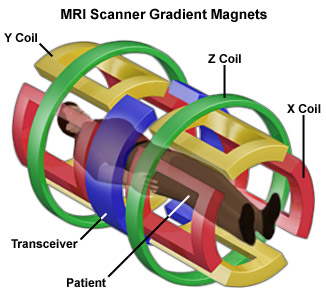
\includegraphics[width=0.7\textwidth]{gradientes}
   \caption{Configuración física de los gradientes de campo magnético. Las estructuras verdes, rojas y amarillas son en realidad conjuntos de cables por los que se pasa una corriente eléctrica, produciendo así un campo magnético secundario que se suma algebraicamente a \Bzero. Tomado de \url{https://nationalmaglab.org}.}
 \label{fig:gradientes}
 \end{figg}
\end{figure}




\section{Selección de rebanada (excitación selectiva)}
De las tres dimensiones que tenemos que codificar, la más sencilla es la que identificaremos como rebanada o corte del objeto. Cuando hablamos de cortes en humanos, consideramos los planos anatómicos clásicos: axial, coronal y sagital. Los cortes axiales atraviesan al sujeto de forma perpendicular a su eje longitudinal (superior-inferior); los coronales lo hacen perpendicular al eje antero-posterior, y los cortes sagitales son paralelos a la línea media. Por convención y por la manera en que la mayoría de los resonadores magnéticos de humanos están construidos, el eje longitudinal del paciente (habitualmente acostado) penetra el túnel del magneto, y se denomina el eje \textit{z}, siendo los ejes \textit{x} y \textit{y} perpendiculares a éste. Para fines didácticos, la mayoría de los ejemplos que se presentan en este capítulo tratan de rebanadas axiales (perpendiculares al eje \textit{z}), a menos que se especifique lo contrario. A partir de la ecuación \ref{eq_LarmorGradientes}, podemos excitar selectivamente a un grupo de spins mediante la aplicación de una radio-frecuencia (RF o \Bone) con un ancho de banda que coincida con las frecuencias de precesión de la zona de interés (Figura \ref{fig:rebanadas}). Recordemos que lograremos perturbar \Mz únicamente si la frecuencia de \Bone es igual a la frecuencia de precesión. Dada la presencia del gradiente del campo magnético, hemos manipulado estas frecuencias, y conocemos el rango (ancho de banda) en el que se encuentran, así que es fácil producir un pulso de RF que contenga las frecuencias calculadas. Todos los spins del cuerpo del paciente están precesando con cierta frecuencia, pero existe un sitio dentro del resonador donde hemos producido un rango de frecuencias específicas, y únicamente los spins en esta región serán perturbados mediante \Bone. Si utilizamos un pulso que desvíe 90\degrees a \Mz, entonces lograremos colocar la totalidad de la magnetización neta en el plano \textit{x,y} en una rebanada, mientras que esto no se logrará en spins que no estén en el sitio de interés.

Las rebanadas o cortes tienen un centro (posición) y un espesor. Estos pueden manipularse mediante tres parámetros: la frecuencia central, el ancho de banda, y la amplitud de $G$ mediante la siguiente relación:
\begin{equation}
 \Delta\omega = \gamma G \Delta{z}
\end{equation}
donde $\Delta\omega$ indica el ancho de banda de la RF, y $\Delta{z}$ indica el grosor de la rebanada. La orientación de $G$ determinará el tipo de corte: si el gradiente se aplica sobre el eje $z$, lograremos una rebanada axial, y si se aplica sobre el eje $x$ lograremos rebanadas sagitales. Es posible hacer cortes oblicuos utilizando trigonometría para usar de manera simultánea los tres juegos de gradientes. La frecuencia central identificará el centro de la rebanada en relación a la ecuación \ref{eq_LarmorGradientes}, mientras que el ancho de banda, en combinación con $G$, determinarán el espesor de la rebanada (Figura \ref{fig:rebanadas_BW}).


\begin{figure}[htb]
 \begin{figg}
   \includegraphics[width=\textwidth]{rebanadas}
   \caption{Excitación selectiva de una rebanada. Tomado de \cite{mcrobbie2007mri}.}
 \label{fig:rebanadas}
 \end{figg}
\end{figure}

\begin{figure}[htb]
 \begin{figg}
   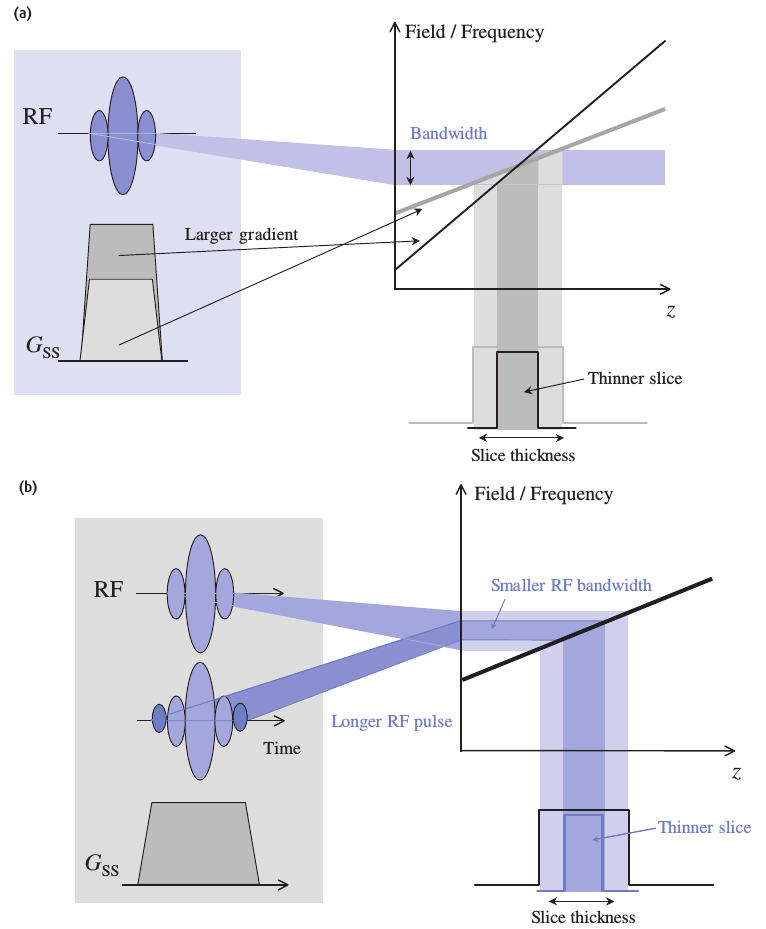
\includegraphics[width=\textwidth]{rebanadas_BW}
   \caption{Control del grosor de la rebanada. La amplitud del gradiente (a) y el ancho de banda del pulso de RF (b) se utilizan para definir el espesor del corte. Tomado de \cite{mcrobbie2007mri}.}
 \label{fig:rebanadas_BW}
 \end{figg}
\end{figure}



\section{Codificación mediante frecuencia}
Una vez que se realizó una excitación selectiva de una rebanada, podemos codificar una de las dos dimensiones restantes mediante la frecuencia de precesión. Este proceso es sencillo, y nuevamente se basa en la frecuencia de Larmour, $\omega$, que depende directamente del campo magnético experimentado, que puede ser modulado linealmente mediante gradientes, tal como se describió en la ecuación \ref{eq_LarmorGradientes}. Imaginemos una imagen de tres pixeles, cada uno con una cantidad total de moléculas de agua, como se observa en la Figura \ref{fig:gradientes2}. Si aplicamos mediante un gradiente una modulación del campo magnético de izquierda a derecha (de 2.99 T a 3.01 T), los spins del cada pixel experimentarán diferentes campos magnéticos entre ellos, y por ende cada uno precesará a una frecuencia dada, que rondará entre 127.075 y 127.925 MHz. 
 
\begin{figure}[htb]
 \begin{figg}
   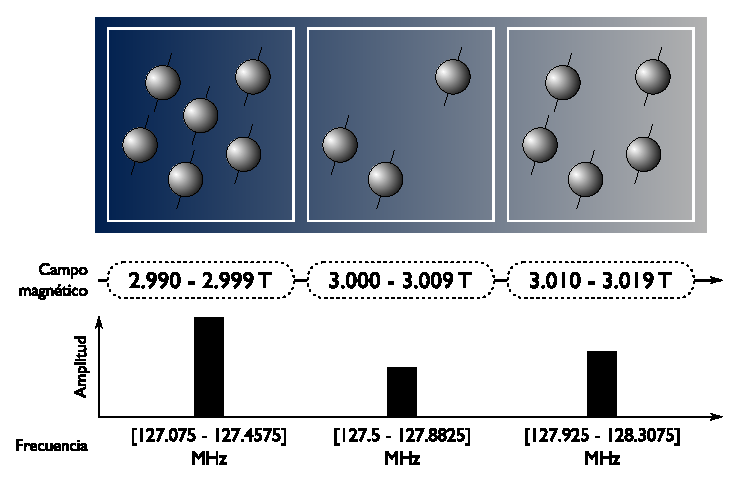
\includegraphics[width=\textwidth]{gradientes2}
   \caption{Codificación espacial mediante frecuencia.}
 \label{fig:gradientes2}
 \end{figg}
\end{figure}

Cuando recibamos la señal de resonancia proveniente de estos spins, ésta contendrá de manera simultánea las frecuencias en todo el rango antes mencionados, y cada frecuencia en este rango estará más o menos representada, dependiendo del número de spins que precesa a esa frecuencia. El ancho de banda que recibiremos está limitado por
\index{Ancho de banda|textbf}
\index{Bandwidth|textbf}

\begin{equation}
 BW = \gamma G (FOV).
 \label{eq_bw_read}
\end{equation}


Por supuesto, la división en tres pixeles es arbitraria y artificial, y la realidad es que se recibirá un enorme número de posibles frecuencias, pero todas ellas dentro del rango entre 127.075 y 127.925 MHz.  Si bien la señal recibida será altamente compleja, afortunadamente podemos analizarla utilizando uno de los tratamientos matemáticos más útiles de todos los tiempos: la transformada de Fourier. Formalmente, ésta postula que toda señal está en realidad formada por la suma de un número de señales periódicas de diferentes frecuencias y fases (Figura \ref{fig:Fourier_decomposition}). Es decir, la transformada de Fourier es como un prisma que descompone a la luz en sus coloridos componentes. A diario nos encontramos con aplicaciones de la transformada de Fourier, como en el ecualizador del sonido de un equipo de reproducción de música, que nos permite controlar la amplitud de rangos de frecuencias organizados en distintas bandas, desde las frecuencias más bajas a la izquierda, hasta las más altas a la derecha (Figura \ref{fig:equalizer}). 

\begin{figure}[htb]
 \begin{figg}
   \includegraphics[width=0.7\textwidth]{Fourier_decomposition}
   \caption{Transformada de Fourier. La curva compleja de color añil puede ser formada mediante la suma de las primeras tres curvas simples sinusoidales.}
 \label{fig:Fourier_decomposition}
 \end{figg}
\end{figure}

\begin{figure}[htb]
 \begin{figg}
   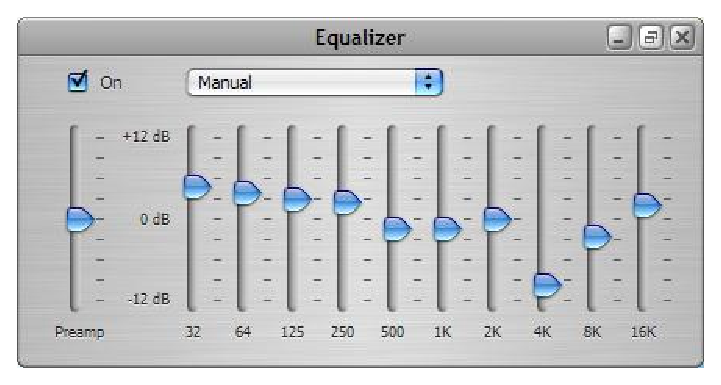
\includegraphics[width=0.7\textwidth]{equalizer}
   \caption{Ecualizador de reproductor de sonido. Cada barra deslizable controla la amplitud de cierto ancho de banda que se reproduce en el sonido.} 
 \label{fig:equalizer}
 \end{figg}
\end{figure}

De hecho, dado que la amplitud de cada frecuencia depende de la cantidad de agua en cada posición, la gráfica de frecuencia y amplitud después de la transformada de Fourier (es decir, el espectro) tendrá una forma muy similar al objeto mismo, como una proyección (Figura \ref{fig:proyeccionFrecuencia}).

\begin{figure}[htb]
 \begin{figg}
   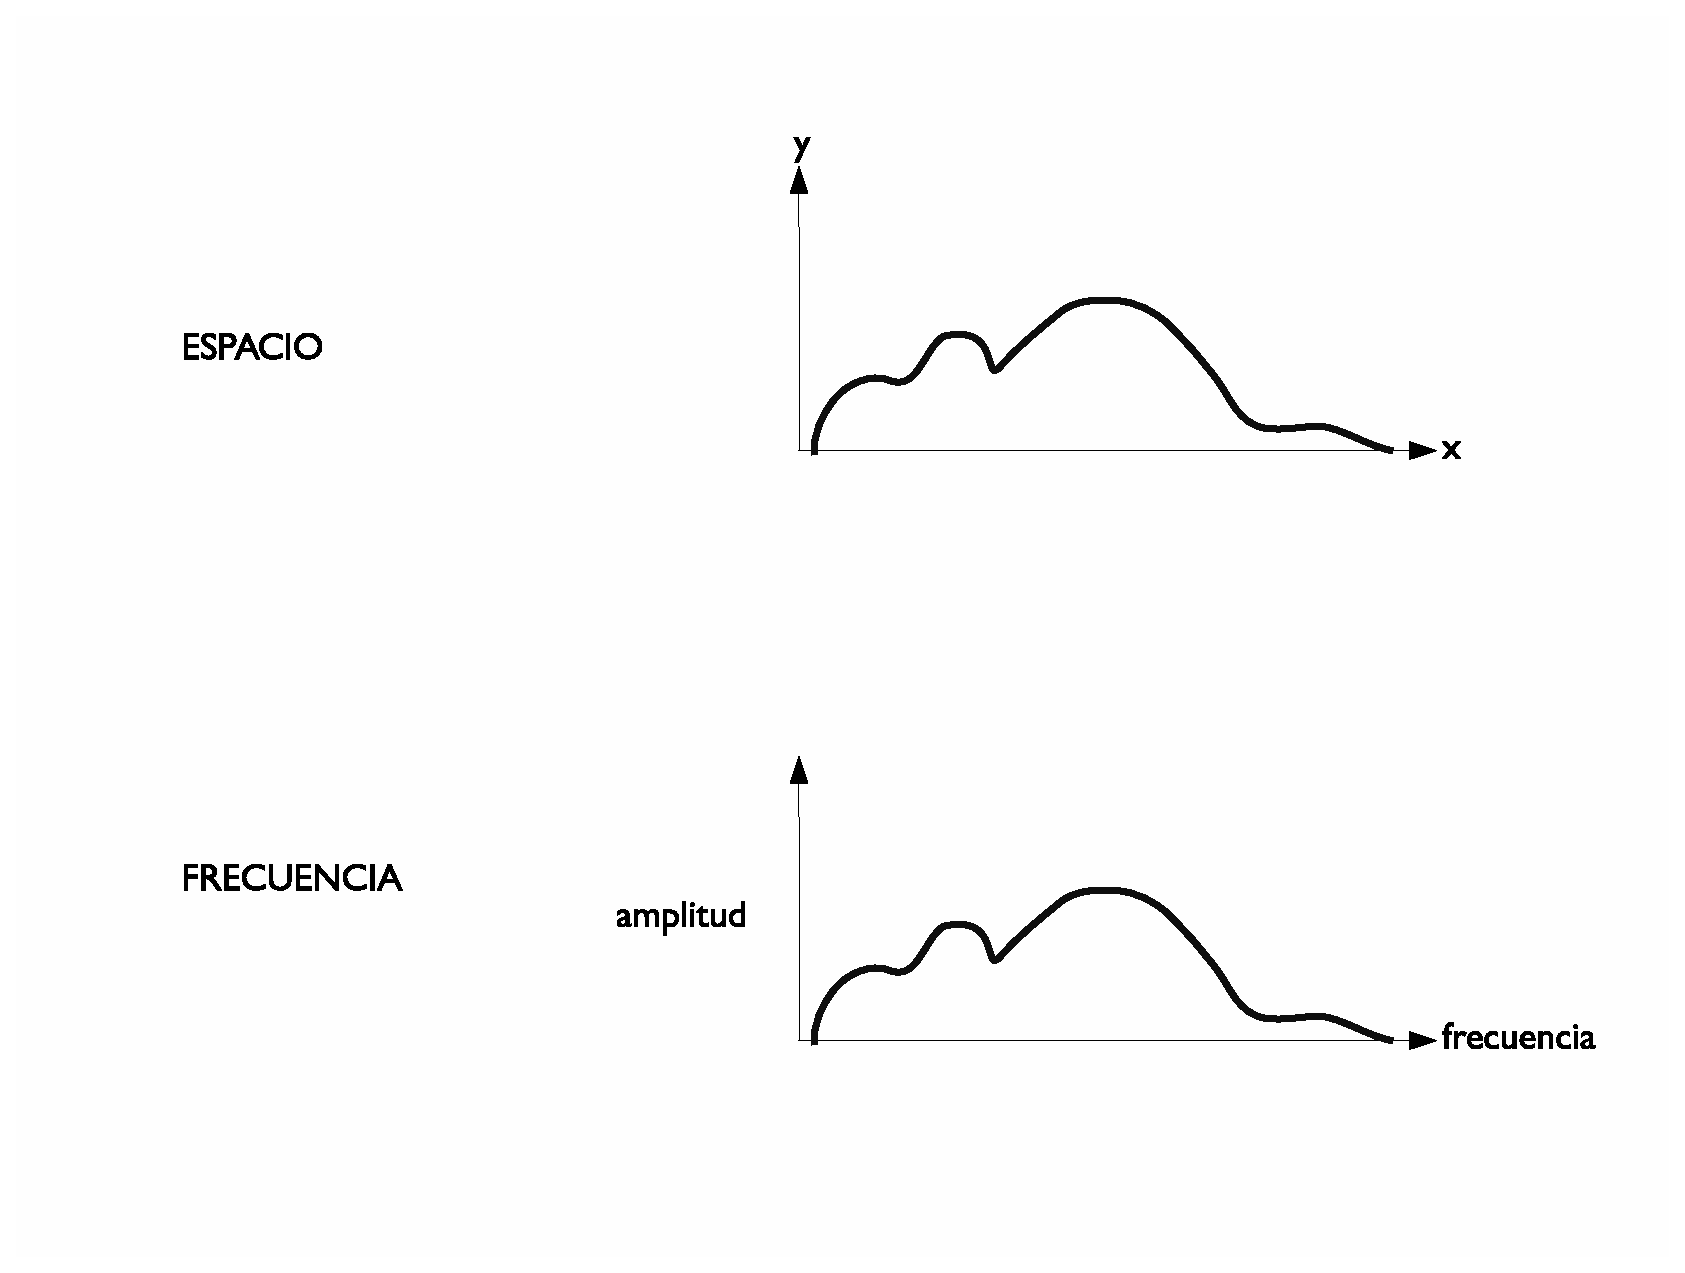
\includegraphics[width=\textwidth]{proyeccionFrecuencia}
   \caption{Proyección del objeto en el espacio de frecuencias. La amplitud de cada una de las frecuencias corresponde a la cantidad de agua presente en el objeto, que precesa a cierta frecuencia.}
 \label{fig:proyeccionFrecuencia}
 \end{figg}
\end{figure}


\section{Codificación mediante fase}
Las primeras dos dimensiones fueron fáciles de codificar: excitación selectiva y codificación por frecuencia y una simple transformada de Fourier. La dimensión que resta es menos intuitiva. Antes de abordar el tema, es importante mencionar que utilizando la codificación de frecuencia, y aprovechando el hecho de que la amplitud de cada frecuencia dibuja la proyección del objeto (Figura \ref{fig:proyeccionFrecuencia}), es posible realizar codificación de la última dimensión si se repite el experimento de codificación por frecuencia, pero cambiando la orientación del gradiente aplicado. En esta situación, la curva amplitud/frecuencia será la proyección del objeto visto desde distintas perspectivas dependientes de la orientación del gradiente. Si se acumulan suficientes proyecciones, se puede reconstruir la imagen en el plano mediante el método de retro-proyección (Funk-Radon) justo como en una tomografía. De hecho, ésta fue la primer técnica de codificación espacial de resonancia magnética, pero ha perdido terreno ante la codificación mediante fase.

Recordemos que una onda periódica (como una sinusoide) tiene tres características: su frecuencia (que es el inverso del periodo), su amplitud y su fase. Dos señales con frecuencia y amplitud idénticas pueden distinguirse si tienen fases distintas (Figura \ref{fig:fases}), y entendemos por fase el momento en que la amplitud pasa por el eje horizontal. La fase se describe en términos de radianes, o grados, pues las ondas sinusoidales son la representación lineal de un movimiento angular (Figura \ref{fig:sine_anim}).


\begin{figure}[htb]
 \begin{figg}
   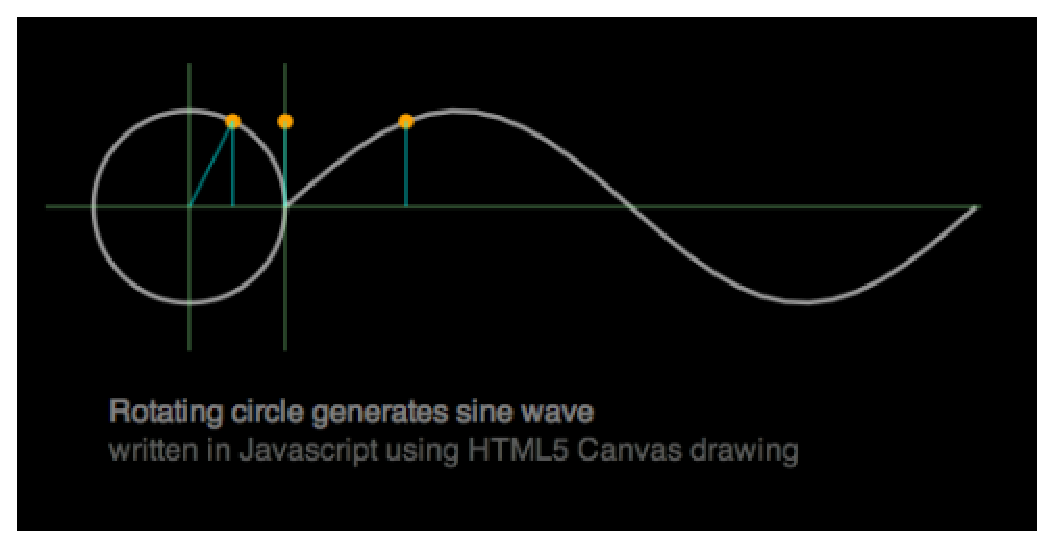
\includegraphics[width=0.7\textwidth]{sine_anim}
   \caption{Representación gráfica de la fase de un movimiento angular. Al rotar la línea radial en el círculo, su proyección sobre el eje de las $x$ representa el seno del ángulo creado. Este puede ser graficado linealmente (a la derecha). En caso de comenzar a graficar a diferentes ángulos, las curvas sinusoides tendrán la misma forma, pero comenzarán antes o después con respecto al eje $x$. Tomado de \url{https://quantblog.wordpress.com/2010/05/26/animated-sine-wave-in-javascript-html5}.}
 \label{fig:sine_anim}
 \end{figg}
\end{figure}

\begin{figure}[htb]
 \begin{figg}
   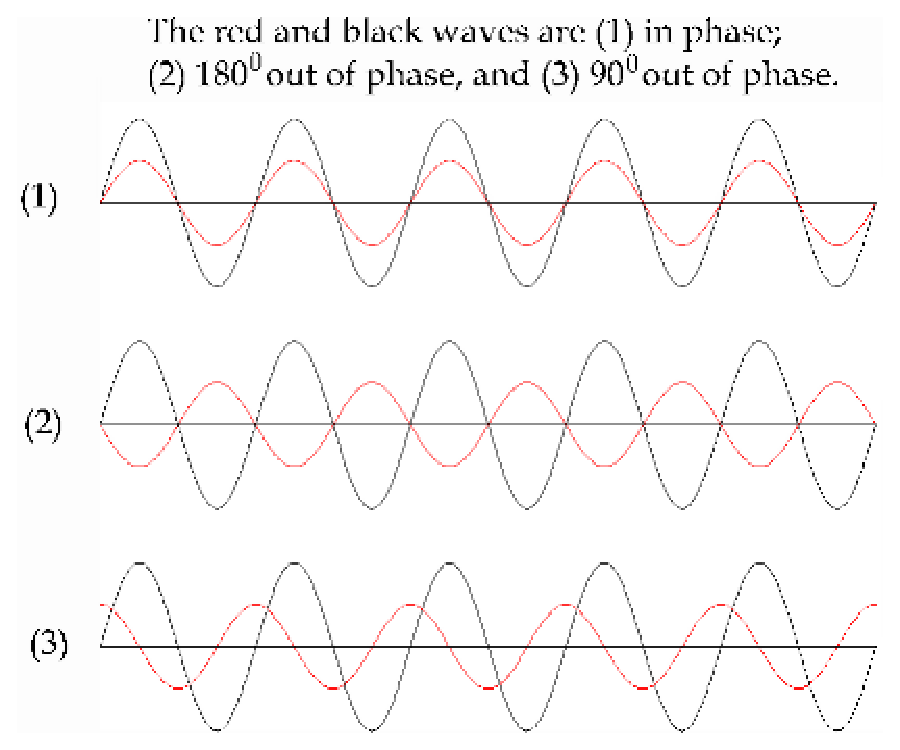
\includegraphics[width=0.7\textwidth]{fases}
   \caption{Tomado de \url{http://www.silcom.com/~aludwig/images/relphase.gif}}.
 \label{fig:fases}
 \end{figg}
\end{figure}

Dejaremos que la amplitud nos hable de la cantidad de agua, y quedó claro que la frecuencia nos puede hablar de una dimensión, así que permitiremos que la fase nos hable de la otra dimensión del plano. Con ésto podremos pasar de la proyección en una dimensión de un objeto, con el consecuente aplanamiento de la segunda dimensión, a la generación de la imagen completa. Si bien nuestra proyección amplitud/frecuencia seguirá siendo cierta, podemos obtener varias proyecciones, cada una con una fase distinta. 

Recordando que la frecuencia de precesión depende del campo magnético experimentado, podemos prender un gradiente del campo magnético  para otorgar distintas frecuencias en una dirección, pero al apagar el gradiente regresaremos a la frecuencia base, $\omega_0$, otorgada por \Bzero. Crucialmente, aunque tras apagar el gradiente todos los spins estén precesando a la misma frecuencia, habrá una diferencia entre sus fases en la dirección en que aplicamos el gradiente. La cantidad de fase que acumulan los spins ($\Delta\omega$) es proporcional a la magnitud del gradiente ($G$),  el tiempo ($t$) que se mantiene prendido y, por supuesto, la localización de los spins con respecto a este gradiente ($r$), de acuerdo a la ecuación \ref{eq_fase}:

\begin{equation}
 \Delta\omega = \gamma G(t) \cdot r
 \label{eq_fase}
\end{equation}


Es importante recalcar que el gradiente de fase debe prenderse y apagarse de manera independiente (habitualmente antes) del gradiente codificador de frecuencia, pues de lo contrario ambos gradientes se sumarían y modificarían de manera oblicua a \Bzero. Es también fundamental que las orientaciones de ambos gradientes sean perpendiculares entre sí. Así como en los problemas de matemáticas de educación secundaria, donde buscamos resolver tres incógnitas para lo que se requieren al menos tres ecuaciones, si queremos codificar el plano dividiéndolo en 128 posiciones verticales, necesitaremos repetir el paso de prender el gradiente codificador de fase al menos 128 veces, variando su amplitud de manera única en cada repetición, otorgando 128 fases distintas. 

La secuencia temporal en la que se juegan los diferentes componentes de excitación y codificación se conoce como \index{secuencia de pulsos} secuencia de pulsos. Recapitulando:

\begin{enumerate}
 \item Un pulso de RF excitador, simultáneo a un gradiente en una dirección ($z$, por ejemplo).
 \item Un pulso breve del gradiente codificador de fase, con cierta magnitud  (*).
 \item Un pulso codificador de frecuencia.
\end{enumerate}
(*) El paso 2 se repite tantas veces como se requiera para lograr mayor resolución, siendo la magnitud del gradiente distinto en cada paso. La señal que se recibe después de cada paso 3 posee distintas fases cada una, y se deben ir digitalizando y almacenando para posteriormente realizar una doble transformada de Fourier. El almacén de estas señales digitalizadas se conoce como \espaciok.


La extensión anatómica que se traduce en imagen se conoce como campo de visión, o más comúnmente como FOV (\emph{Field of view}) \index{FOV}, y tiene dos dimensiones más un cierto espesor de la rebanada. El usuario elige cuál de las dos dimensiones será codificada mediante frecuencia y cuál por fase. Asímismo, el usuario elige el número de particiones que tiene el FOV, lo que se traduce en la resolución de la imagen. Por ejemplo, el FOV puede dividirse en 128 columnas y 128 renglones. La resolución, entonces, se calcula simplemente:

\begin{eqnarray}
 Res_x = FOV_x / N_{frec}\\
 Res_y = FOV_y / N_{fase}
\end{eqnarray}
donde $Res_x$ y $Res_y$ son las dimensiones $x$ y $y$ de los pixeles resultantes, $FOV_x$ y $FOV_y$ son las dimensiones del FOV, y $N_{frec}$ y $N_{fase}$ es el número de particiones de las dos direcciones de codificación espacial. 

En el caso de la dirección codificada mediante frecuencia, cada pixel contiene un cierto rango de frecuencias (ancho de banda) que depende de la magnitud de $G$ y el FOV, de acuerdo a la ecuación \ref{eq_bw_read}. El total de las frecuencias en este ancho de banda se dividirá en el número de particiones del $FOV_{x}$. Si $G$ se mantiene constante y modificamos el número de particiones $N_{frec}$, el ancho de banda total no se modificará, pero sí lo hará en cada pixel. Es útil imaginar a cada pixel como un contenedor de diferentes frecuencias, y que cada pequeño paquete de frecuencias se asocia a una localización espacial. Lo anterior se aplica de forma idéntica a la dirección codificada por fase, con la particularidad de que cada uno de estos paquetes de frecuencias se logró mediante experimentos sucesivos en los que se modificó paulatinamente la magnitud del gradiente de fase.


Existen límites físicos y prácticos acerca de la máxima resolución alcanzable. Por ejemplo, la potencia máxima de los gradientes limitan la resolución, y siempre se debe recordar que mientras más pequeño sea el pixel, menos cantidad de moléculas de agua contendrá, lo que llevará a una degradación de la imagen resultante.


\section{El \espaciok}
\index{Espacio k|textbf}
Toda la información recibida por cada rebanada, en forma digital, se guarda en una matriz que tiene dos ejes: \kx y \ky. Las frecuencias aumentan de izquierda a derecha en el eje \kx y las fases en el eje vertical \ky. La matriz tiene tantas celdas celdas como el número de pixeles a reconstruir.  El nombre de este espacio se debe a que habitualmente se utiliza la letra $k$ para designar el número de periodos de una onda sinusoidal por unidad de distancia (habitualmente metros). Por ejemplo, una onda que presenta dos periodos en cada metro tiene una $k = 2 m^{-1}$.

Curiosamente, no existe una correspondencia punto a punto entre cada celda del \espaciok con cada pixel de la imagen. Por el contrario, cada celda del \espaciok contiene información de toda la imagen de manera simultánea, y cada pixel de la imagen está representado en todo el \espaciok. Cada celda $k_{x,i},k_{y,j}$ representa la amplitud de la frecuencia $i$ con fase $j$. La magnitud (intensidad) en cada celda del \espaciok indica qué tanto una cierta frecuencia y orientación está incluida en la imagen. En un ejercicio mental, podemos imaginar que ``pintaremos'' una imagen pero, en lugar de usar pinceles, usaremos una serie de sellos (o esténciles), todos de las mismas dimensiones (Figure \ref{fig:kspace_stencils}). Cada uno de estos sellos deja estampada una cierta frecuencia (cuántas rayas hay por cada cm, por ejemplo), y en qué orientación está dicha frecuencia (a cero grados, a 45 grados, etc). Algunos sellos los estamparemos fuertemente y con mucha tinta, mientras que otros los estamparemos con sutileza. En la medida en que los distintos sellos se sumen, emergerá nuestra imagen. El ejercicio anterior es análogo a lo que sucede en la corteza visual de los primates: existen neuronas que responden preferencialmente a barras luminosas con cierta frecuencia y orientación, y responden menos a otras frecuencias/orientaciones. Cada una de estas neuronas es un análogo de una celda del \espaciok.


\begin{figure}[htb]
\begin{figg}
   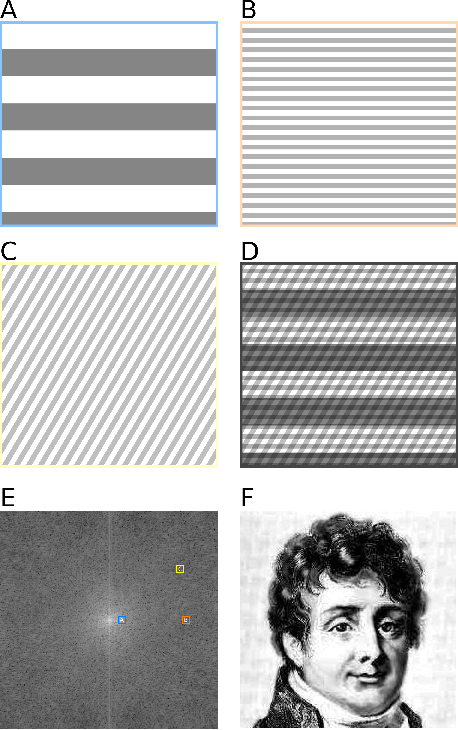
\includegraphics[width=0.6\textwidth]{kspace_stencils}
   \caption{Cada celda del \espaciok representa la intensidad con la que una cierta frecuencia y orientación está presente en la imagen (A-C). En D se muestra la suma de tres celdas del \espaciok. La totalidad del \espaciok se muestra en E, indicando las tres celdas cuya contribución a la imagen se muestran en A-C. La imagen resultante al utilizar todos los puntos del \espaciok de manera simultánea está en F (Mounsier Fourier, 1768-1830). }
 \label{fig:kspace_stencils}
 \end{figg}
\end{figure}



El \espaciok contiene dos juegos de señales: las codificadas mediante el gradiente de frecuencia (didácticamente $k_x$, aunque ésto es arbitrario), y las codificadas mediante el gradiente de fase (didácticamente $k_y$) (Figura \ref{fig:kspace_viz}). Lo único que resta para traducir en información espacial este conjunto de frecuencias es realizar la transformada de Fourier, que en este caso se realiza en dos dimensiones. Analíticamente, la transformada de Fourier es complicada y computacionalmente lenta, por lo que existen algoritmos que aceleran la obtención de las frecuencias que componen un grupo de señales complejas, siendo la más utilizada la transformada rápida de Fourier. Estos algoritmos suelen funcionar más eficientemente si las dimensiones del \espaciok son potencias de 2; esta es la razón por la que habitualmente las imágenes tienen un número de pixeles como 128\texttimes128 o 512\texttimes512.


\begin{figure}[htb]
 \begin{figg}
   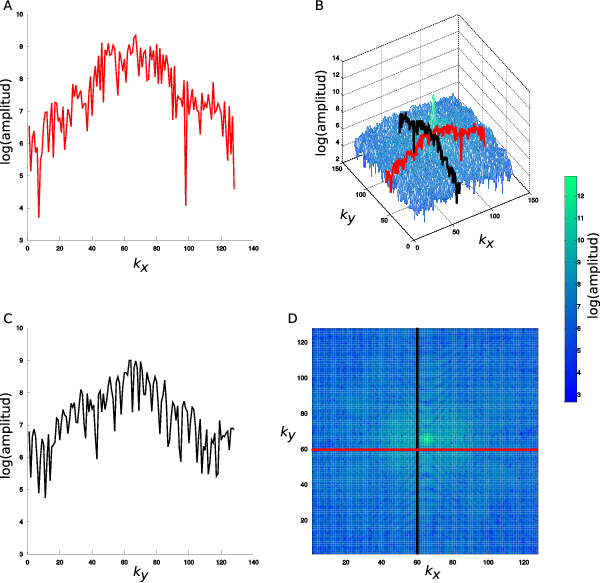
\includegraphics[width=0.7\textwidth]{kspace_viz}
   \caption{Espacio $k$. Por cada codificación mediante el gradiente de fase se obtiene una señal (A). Cada señal es digitalizada y ordenada de acuerdo a la magnitud del gradiente de fase (B), y puede ser visualizada como una matriz de datos (B y D). Al unir los puntos en las columnas del \espaciok se obtienen las señales de la segunda dimensión, una por columna; se ejemplifica una de ellas en el panel C. Las líneas roja y negras en B y D representan las señales mostradas en A y C, respectivamente. D equivale a una vista superior de los datos presentados en B.}
 \label{fig:kspace_viz}
 \end{figg}
\end{figure}



Como se ve en la Figura \ref{fig:kspace_stencils}, el centro del \espaciok contiene información acerca de las bajas frecuencias espaciales (poca alternancia de negro/blanco a lo largo de la imagen real), mientras que las orillas del \espaciok tienen información acerca de altas frecuencias espaciales. Si obliteramos la información contenida en las orillas del \espaciok (convertimos los valores en cero) y realizamos la transformada de Fourier correspondiente, la imagen resultante será una versión borrosa de la original, pero se notará claramente que existen distintas estructuras con niveles de intensidad francamente diferentes (Figura \ref{fig:casos_espaciok}). Por el contrario, si obliteramos la información central del \espaciok, entonces veremos las estructuras de alta frecuencia espacial, es decir, los bordes de las estructuras de nuestra imagen, pero tendremos poco contraste entre estructuras. Además, existe una simetría conjugada en los ejes vertical y horizontal de este espacio, por lo que parece que se mirara a sí mismo en el espejo. Esto da características singulares al \espaciok que pueden ser explotadas ampliamente. Por ejemplo, es posible generar una imagen a partir de poco más de la mitad del \espaciok, lo que significa que podemos obviar la necesidad de adquirir cada uno de sus renglones, lo que nos ahorraría tiempo en la adquisición de la imagen; en efecto, esta es una técnica muy utilizada en la práctica diaria. Por otra parte, algunos algoritmos de compresión de imagen (JPEG, por ejemplo), utiliza esta estrategia para reducir la cantidad de información que se almacena en el disco, sufriendo mínimas consecuencias en la imagen reconstruida a partir de esta información parcial.


\begin{figure}[htb]
 \begin{figg}
   \includegraphics[width=\textwidth]{casos_espaciok}
   \caption{Características del \espaciok. En A se presenta la totalidad del \espaciok correspondiente a la imagen del panel E. A los datos presentados en A se les convirtió a ceros artificialmente su información contenida en toda la periferia (B), lo que genera una imagen con alto contenido de contraste, pero difusa (F). El ejercicio reverso (C) muestra que la periferia del \espaciok guarda la información relativa a los bordes de la imagen (G). Por último, poco más de la mitad del \espaciok (D) es suficiente para reconstruir la imagen con poca degradación (H).}
 \label{fig:casos_espaciok}
 \end{figg}
\end{figure}


Siguiendo la manera en que postulamos previamente, el \espaciok se llena línea por línea, o unas cuantas líneas por vez. Como se verá en el capítulo \ref{chapter_secuencias}, existen varias formas de llenar el \espaciok, no necesariamente cartesianas.










\chapter{Secuencias de pulsos básicas}
\chapterprecis{\noindent \noindent Gilberto Rojas Vite\\Instituto de Neurobiología\\UNAM, Campus Juriquilla}
\label{chapter_secuencias}

\textbf{NOTA: Las figuras de este capítulo son temporales.}


\section{Introducción}
Una secuencia de pulsos se refiere al orden cronológico y las características de cada uno de las manipulaciones que se hacen a un sistema de spins con el fin de producir una señal interpretable. En el caso de la realización de una imagen, se refiere a la temporalidad, orden, y parámetros de la manipulación de los gradientes del campo magnético, así como la presencia de radio-frecuencias específicas con fines de generación de contraste y codificación espacial. Habitualmente se denomina \textit{protocolo} \index{protocolo} a una serie de adquisiciones de imagen mediante distintas secuencias de pulso a lo largo de una sesión de imagen.

Si bien la mayoría de los parámetros de las diferentes manipulaciones tienen interacciones entre sí, pueden considerarse manipulaciones específicas para generación de contraste, y otras para codificación espacial; existen un gran número de combinaciones especiales de parámetros para cada uno de esos fines, y en muchas ocasiones es posible hacer combinaciones de tipos de contraste específicos con métodos particulares de codificación especial. En otras palabras, a veces es útil dividir las secuencias de pulsos en segmentos con fines específicos, y estos segmentos pueden utilizarse como \textit{plugins}. Por ejemplo, uno puede realizar una imagen con contraste T2 mediante codificación espacial ecoplanar o turbo-spin eco (TSE), o hacer una imagen TSE con contraste T1.

\section{La secuencia de pulsos más básica: FID.}
\index{FID (\textit{free-induction decay})|textbf}
El decaimiento por inducción libre, conocido como FID (\textit{Free Induction Decay}) es la secuencia de pulsos más simple. La FID refiere a la señal que se recibe después de realizar un pulso de radiofrecuencia (RF). Detallamos: El vector resultante de los spins de la muestra que se encuentra en el resonador se alinea respecto de \Bzero (fig. \ref{fig:seq_vectorResultante}), o el eje $z$, por lo que lo denominamos \Mz. En este momento nosotros no tenemos señal alguna de nuestra muestra, pues sólo podemos obtener señal de los vectores que se encuentren sobre el eje $x$. Esto se debe a que nuestra antena (fig. \ref{fig:seq_antena}) sólo va a recibir la señal ubicada en dicho eje. 


\begin{figure}[htb]
\begin{figg}
   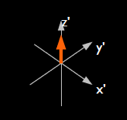
\includegraphics[width=0.5\textwidth]{vite_01}
   \caption{Vector resultante alineado respecto de \Bzero.}
 \label{fig:seq_vectorResultante}
 \end{figg}
\end{figure}

\begin{figure}[htb]
\begin{figg}
   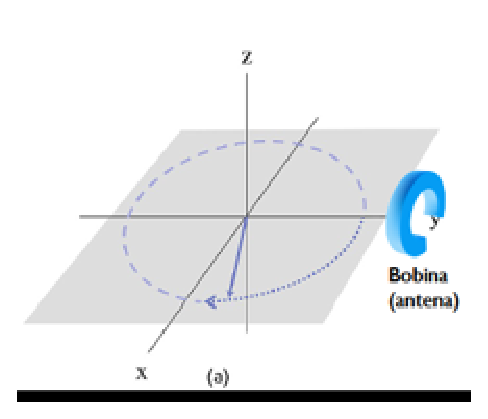
\includegraphics[width=0.5\textwidth]{vite_02}
   \caption{Vector resultante alineado respecto de \Bzero.}
 \label{fig:seq_antena}
 \end{figg}
\end{figure}



Por tanto, para obtener señal de nuestra muestra necesitamos que haya algún vector sobre el eje $x$. Para lograr esto realizaremos un pulso excitador (radiofrecuencia, RF) que cambie la orientación de $M$ del eje $z$ al eje $x$ o plano $x,y$ (es decir \Mz se convierte en \Mxy. Fig \ref{fig:seq_Mx}). Esta perturbación de nuestro sistema inicial permitirá que nuestra antena pueda captar la señal.



\begin{figure}[htb]
\begin{figg}
   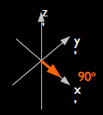
\includegraphics[width=0.5\textwidth]{vite_03}
   \caption{Vector resultante sobre el eje $x$.}
 \label{fig:seq_Mx}
 \end{figg}
\end{figure}


Ahora bien, al apagar el pulso de RF, la señal que hemos recibido irá decayendo debido al fenómeno de relajación transversal. De tal modo que, después de determinado tiempo, podemos decir que $M$ regresará al eje $z$ y volveremos a quedarnos sin señal (fig. \ref{fig:seq_relax}). 

\begin{figure}[htb]
\begin{figg}
   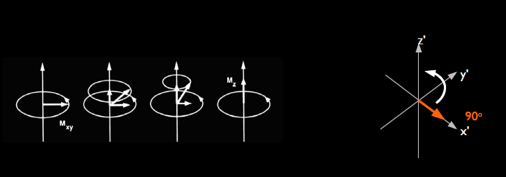
\includegraphics[width=0.75\textwidth]{vite_04}
   \caption{Regreso al estado de reposo.}
 \label{fig:seq_relax}
 \end{figg}
\end{figure}
 


En el proceso que va desde la perturbación de $M$ hasta su regreso al estado de reposo, obtenemos señal a través de la corriente que es inducida en nuestra antena. Cuando $M$ es perturbado y se encuentra sobre el eje $x$, se encuentra precesando y cada vez que pasa por nuestra antena envía electrones. Gracias a este envío de electrones nosotros obtenemos señal. La señal de la que tanto hemos hablado refiere a una onda sinusoide que tiene su mayor amplitud justo después del pulso de RF y que va decayendo conforme pasa el tiempo. El decaimiento se deben enfatizamos, a que el regreso de $M$ al eje $z$ implica una reducción del componente transversal (el único que podemos medir directamente por medio de nuestra antena; fig. \ref{fig:seq_fid}). 

\begin{figure}[htb]
\begin{figg}
   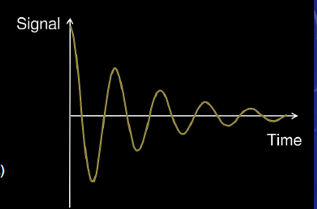
\includegraphics[width=0.5\textwidth]{vite_05}
   \caption{Señal sinusoidal amortiguada.}
 \label{fig:seq_fid}
 \end{figg}
\end{figure}

\section{Secuencias de pulsos generadoras de contraste}

\subsection{Eco de spin}
\index{Eco de spin|textbf}
\index{TE (Tiempo de eco)|textbf}
El eco de spin (SE), como la FID, comienza con un pulso de  RF de 90\degrees. Sin embargo, la diferencia estriba en que agregamos otro pulso de 180\degrees. Lo que lograremos con esto es recuperar la señal que se iba perdiendo con la FID, gracias a un refasamiento de los spins. 

Una vez que hemos realizado un pulso de RF de 90\degrees (fig. \ref{fig:seq_spinecho}-b), el componente transversal de nuestro vector resultante se va reduciendo, debido al desfase de los spins (fig. \ref{fig:seq_spinecho}-c), y por tanto obtenemos menos señal. Una forma de recuperar esta señal es a través de la inducción de un pulso de 180\degrees (fig. \ref{fig:seq_spinecho}-d). 
Cuando realizamos el segundo pulso invertimos el escenario. Los spins se encuentran en una nueva situación (fig. \ref{fig:seq_spinecho}-e) que permitirá que vuelvan a refasarse (fig. \ref{fig:seq_spinecho}-f) y podamos obtener señal. Esta señal recuperada se llama eco y el tiempo que ocurre es proporcional al tiempo entre nuestros pulsos de radiofrecuencia. Precisamente, el tiempo de eco será igual al tiempo transcurrido entre el primer pulso y el eco generado (fig. \ref{fig:seq_TE}).



\begin{figure}[htb]
\begin{figg}
   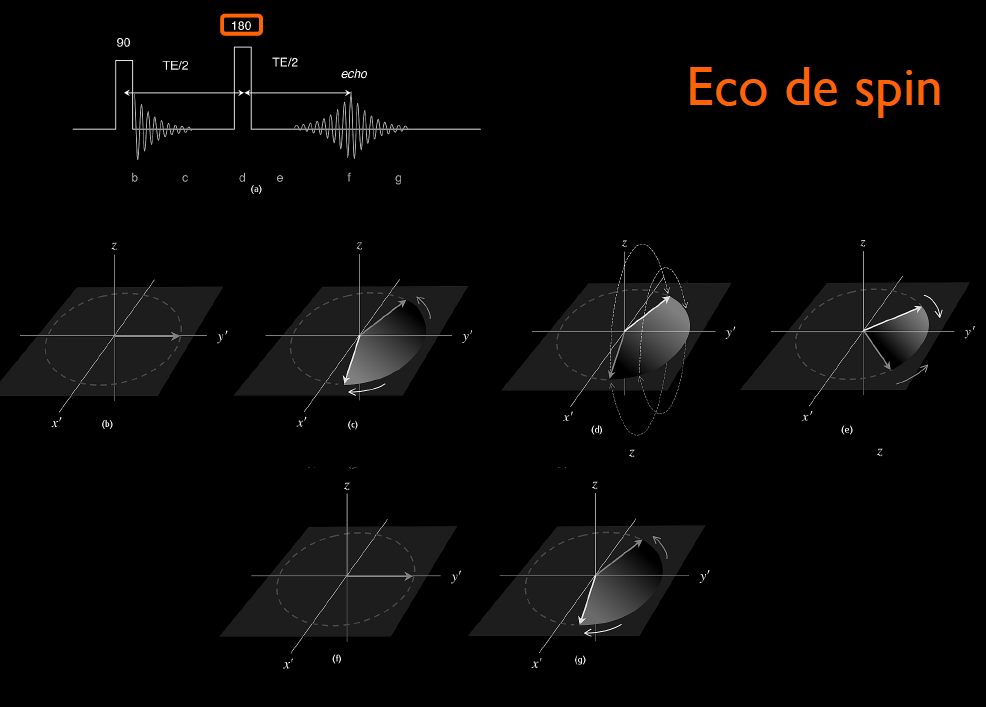
\includegraphics[width=0.75\textwidth]{vite_06}
   \caption{Eco de spin.}
 \label{fig:seq_spinecho}
 \end{figg}
\end{figure}


\begin{figure}[htb]
\begin{figg}
   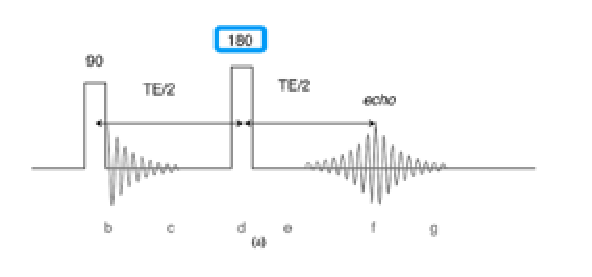
\includegraphics[width=0.75\textwidth]{vite_07}
   \caption{Tiempo de eco.}
 \label{fig:seq_TE}
 \end{figg}
\end{figure}

\subsection{Eco de gradiente }
\index{Eco de gradiente|textbf}
Al igual que el eco de spin, el eco de gradiente (GRE) comienza con un pulso excitador con un ángulo $\alpha$. El ángulo del pulso puede ser de 90\degrees, pero esto dependerá de la información que queramos obtener. Un ángulo de 90\degrees nos permitiría obtener una imagen potenciada a T1, mientras que un ángulo de 10\degrees, podría generar una imagen con información sobre la densidad de protones. 

Después del pulso de RF, se activan dos dos gradientes que nos permitirán generar el eco y la recuperación de la señal correspondiente. El primer gradiente acelera el desfasamientos de los spins. El segundo gradiente tiene la misma amplitud que el primero, pero con signo opuesto. La actividad de este gradiente permite el refase de los spins desfasados inicialmente y la obtención del eco (fig. \ref{fig:seq_GRE}).

Las secuencias con GRE son más rápidas que las generadas por un SE convencional. Sin embargo, la consecuencia de esto son imágenes con mayores artefactos. Esto se debe a que en las secuencias SE, el segundo pulso de 180\degrees ayuda a corregir las heterogeneidades externas. 


\begin{figure}[htb]
\begin{figg}
   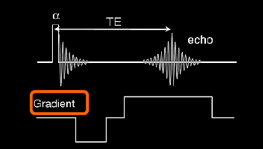
\includegraphics[width=0.75\textwidth]{vite_08}
   \caption{Representación gráfica del eco de gradiente.}
 \label{fig:seq_GRE}
 \end{figg}
\end{figure}


\subsection{Inversión-recuperación}
\index{IR (inversión-recuperación)|textbf}
El pulso de inversión-recuperación (IR) puede ser considerado un SE convencional, al que se le ha agregado antes un pulso de RF de 180\degrees (fig. \ref{fig:seq_IR}). El tiempo entre el pulso de 180\degrees y el de 90\degrees es conocido como tiempo de inversión (TI), el único cambio que agregaríamos a los parámetros de tiempo presentes en el SE (TE y TR). 


\begin{figure}[htb]
\begin{figg}
   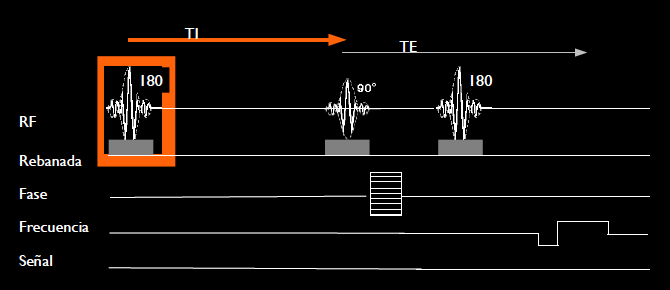
\includegraphics[width=0.75\textwidth]{vite_09}
   \caption{El pulso de inversión-recuperación en una secuencia de pulsos. }
 \label{fig:seq_IR}
 \end{figg}
\end{figure}




La utilidad del pulso IR se ve reflejada en la posibilidad de generar un mayor contraste en imágenes T1 (fig. \ref{fig:seq_RealIR}), así como la supresión de ciertos elementos de nuestra imagen (fig. \ref{fig:seq_supresion}). 

\begin{figure}[htb]
\begin{figg}
   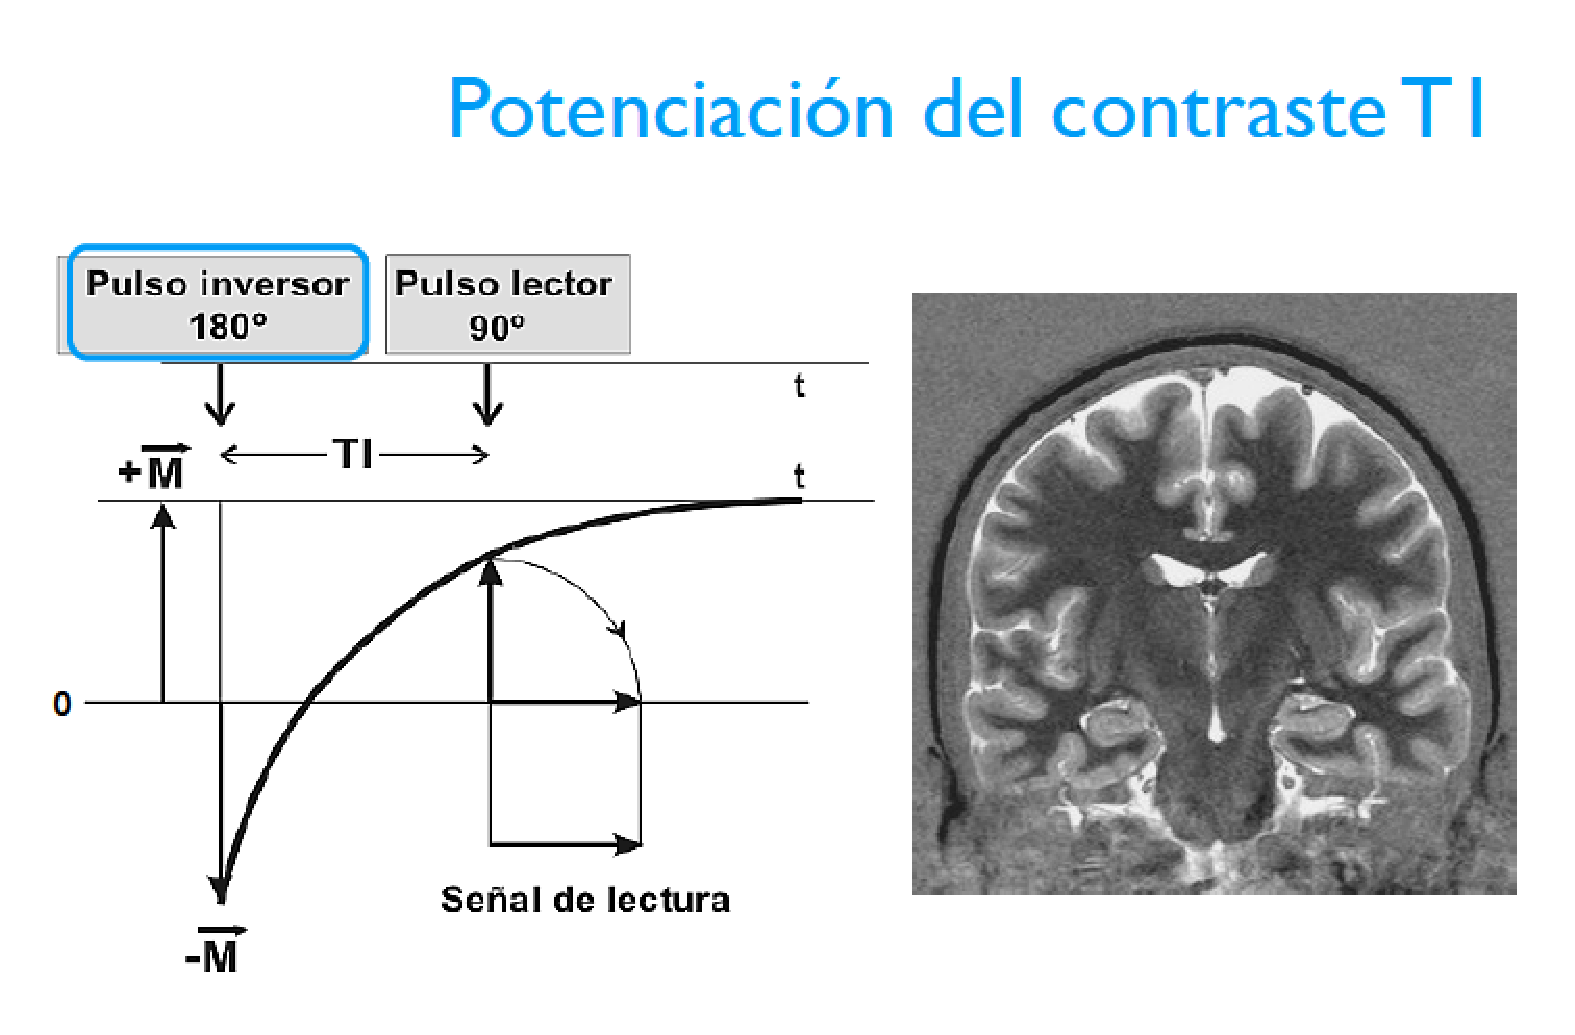
\includegraphics[width=0.75\textwidth]{vite_10}
   \caption{Potenciación del contraste T1 a través de un pulso inversor. En el momento que se aplica el pulso de 90\degrees (pulso lector), las diferencias en el tejido marcadas por TI serán más evidentes gracias al tiempo extra que se ha dado para la relajación de los tejidos.}
 \label{fig:seq_RealIR}
 \end{figg}
\end{figure}

\begin{figure}[htb]
\begin{figg}
   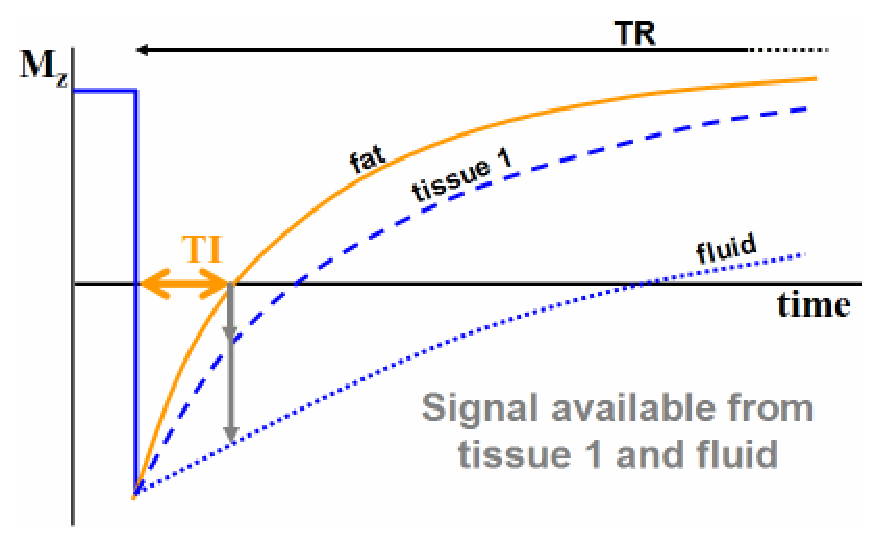
\includegraphics[width=0.75\textwidth]{vite_11}
   \caption{ El TI nos puede ayudar a la supresión de elementos, si conocemos el tiempo de inversión necesario para realizar nuestro pulso lector cuando la señal proveniente de un elemento no tiene presencia sobre el eje $z$. En este caso, la señal de la grasa quedaría suprimida.}
 \label{fig:seq_supresion}
 \end{figg}
\end{figure}




Esta característica del pulso de inversión-recuperación ha ayudado al desarrollo de otras técnicas como FLAIR (\textit{Fluid Attenuated Inversión Recovery})\index{FLAIR|textbf}, que permite la supresión de fluidos (fig. \ref{fig:seq_FLAIR}); y STIR (\textit{Short time inversión Recovery}), la cual permite la atenuación de la grasa (fig. \ref{fig:seq_STIR})\index{STIR|textbf}. En las siguientes figuras podemos encontrar ejemplos de estas herramientas:



\begin{figure}[htb]
\begin{figg}
   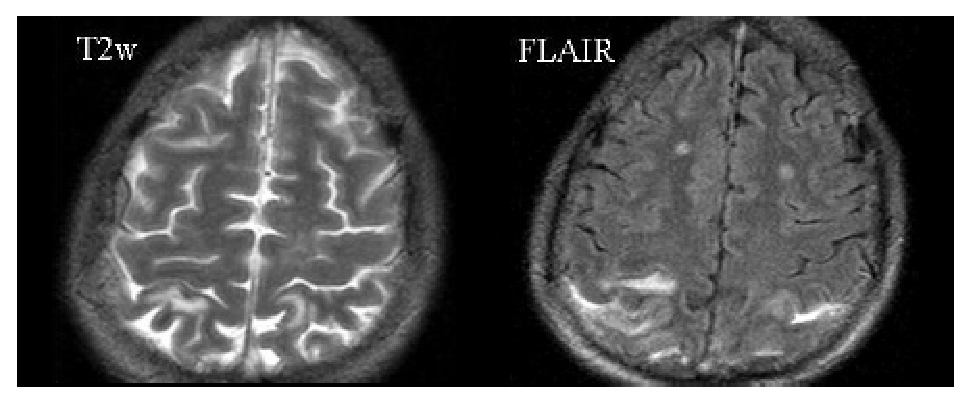
\includegraphics[width=0.75\textwidth]{vite_13}
   \caption{FLAIR. En la parte de la izquierda tenemos una T2 normal. En la imagen de la derecha podemos ver la supresión de las intensidades por FLAIR.}
 \label{fig:seq_FLAIR}
 \end{figg}
 \end{figure}
 
 
\begin{figure}[htb]
\begin{figg}
   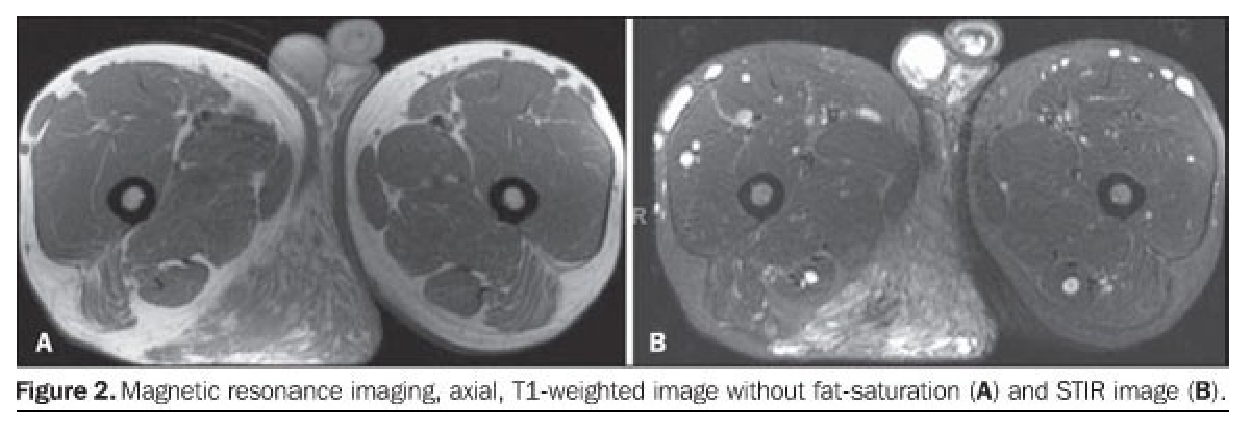
\includegraphics[width=0.75\textwidth]{vite_12}
   \caption{STIR. La imagen de la izquierda es una T1 normal. La imagen de la derecha ha sido obtenida con STIR.}
 \label{fig:seq_STIR}
 \end{figg}
\end{figure}



\section{6.3. Secuencias de pulsos para codificación espacial}

\subsection{Llenado serial del \espaciok}
El llenado serial del \espaciok implica llenar una línea por cada TR, sin saltar líneas, como se muestra en la  figura \ref{fig:seq_kspacelinear}.



\begin{figure}[htb]
\begin{figg}
   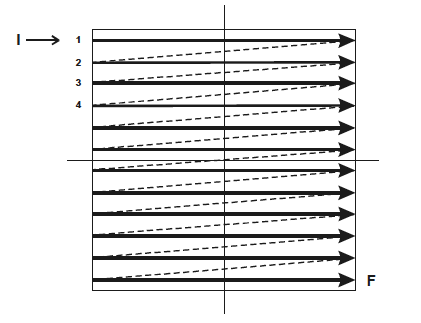
\includegraphics[width=0.75\textwidth]{vite_14}
   \caption{Llenado serial del \espaciok.}
 \label{fig:seq_kspacelinear}
 \end{figg}
\end{figure}


Esta ha sido la forma clásica de llenar el \espaciok. Sin embargo, esto demora mucho la adquisición de imágenes, por lo que nuevas técnicas de llenado del \espaciok han surgido para optimizar los tiempos de obtención. 

\subsection{Secuencias optimizadas para el llenado del \espaciok}
En la actualidad existen técnicas que nos permiten llenar el \espaciok con gran rapidez. Si bien existen una gran variedad de ellas, en esta sección nos enfocaremos a la descripción del turbo-spin eco, el multi-eco y las imágenes ecoplanares. 

\subsubsection{Turbo-spin eco}
\index{Turbo-spin echo|textbf}
El turbo-spin eco (TSE), a diferencia del eco de spin, aprovecha el ``tiempo muerto'', después de la adquisición del eco, para llenar más líneas del \espaciok en menos tiempo, lo cual representa una clara ventaja en comparación con el llenado serial que podemos obtener con una secuencia convencional.
La forma en que se puede lograr esto es a través de un tren de ecos. Después de la secuencia 90-180-eco, es posible el refasamiento de la señal con la introducción de otro pulso de 180\degrees, y así sucesivamente siempre que tengamos señal que recuperar. Para que esto tenga la utilidad deseada resulta necesario hacer un cambio en los gradientes codificadores de fase para que sea posible llenar una línea de \espaciok diferente (fig. \ref{fig:seq_TSE}).


\begin{figure}[htb]
\begin{figg}
   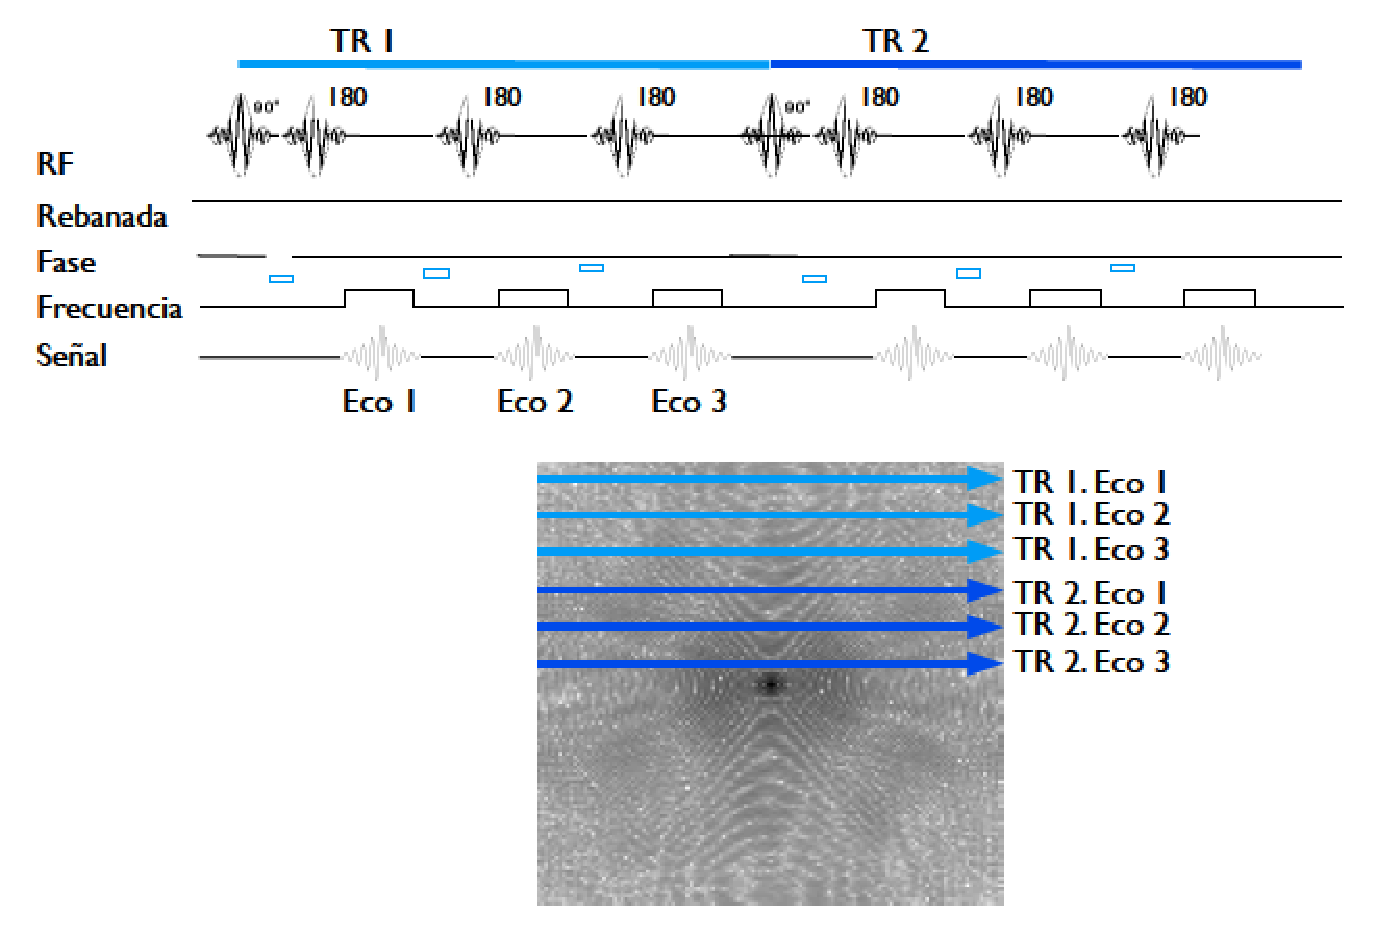
\includegraphics[width=0.75\textwidth]{vite_15}
   \caption{Secuencia turbo-spin eco. En esta secuencia se han llenado tres líneas distintas de \espaciok por cada TR.}
 \label{fig:seq_TSE}
 \end{figg}
\end{figure}




\subsubsection{Multi-spin eco}
\index{Multi-spin echo|textbf}
En el multi-spin eco (MSE) llenamos la misma línea de \espaciok, pero para diferentes imágenes, a diferencia del TSE que llenábamos varias líneas de \espaciok, pero para una misma rebanada.  La ventaja del uso de la secuencia MSE es que podemos ir llenando el \espaciok de imágenes con un distinto contraste, dictado para la diferencia entre los tiempos de eco (fig. \ref{fig:seq_MSE}).



\begin{figure}[htb]
\begin{figg}
   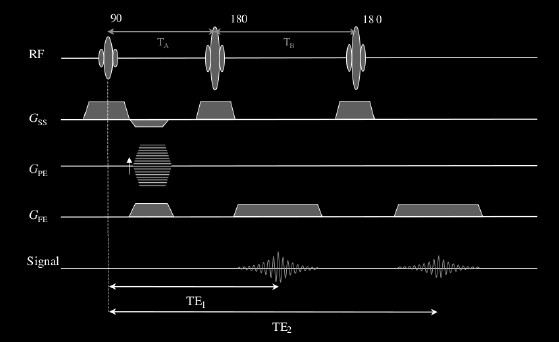
\includegraphics[width=0.75\textwidth]{vite_16}
   \caption{Secuencia multi-spin eco.}
 \label{fig:seq_MSE}
 \end{figg}
\end{figure}



\subsubsection{Imágenes ecoplanares: EPI y multi-shot EPI}
\index{EPI|textbf}
La técnica de imágenes ecoplanares (EPI) es muy poderosa, pues nos permite llenar el espacio-K en un solo TR. Por tanto, podemos tener la información necesaria de nuestra rebanada en un tiempo de adquisición que ronda en los 40 ms.  En la secuencia clásica se parte de un pulso excitador, generalmente de 90. Posteriormente, se generan los ecos necesarios para llenar el \espaciok (fig. \ref{fig:seq_EPI}). El llenado del \espaciok, por otra parte, se ve optimizado al hacerse en zig-zag (16b), debido a que se acorta el tiempo de reposicionamiento de nuestros gradientes. 

Las imágenes obtenidas por EPI nos permiten una adquisición muy veloz. Sin embargo, este factor esta limitado por la atenuación de la señal, con la consiguiente perdida de calidad en nuestras imágenes. Una solución a esto, puede ser llenar el espacio en más de un TR, lo que se conoce como Multi-shot EPI. 


\begin{figure}[htb]
\begin{figg}
   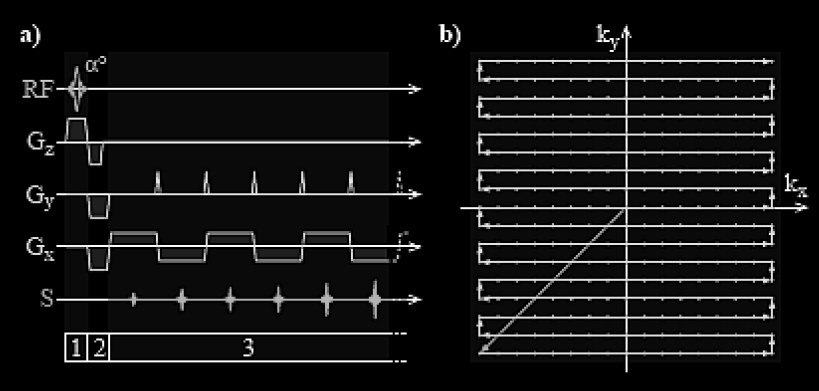
\includegraphics[width=0.75\textwidth]{vite_17}
   \caption{En la imagen de la izquierda se puede apreciar la secuencia de pulsos básica para una imagen ecoplanar. En la imagen de la derecha se muestra esquemáticamente la forma de llenado en zigzag del \espaciok.}
 \label{fig:seq_EPI}
 \end{figg}
\end{figure}







\chapter{Hardware: Campo magnético principal, gradientes y antenas}
\chapterprecis{\noindent SIN AUTOR}
\label{chapter_hardware}


\chapter{Aspectos de seguridad}
\chapterprecis{\noindent Erick Pasaye, Javier Sánchez López \\
                         Instituto de Neurobiología\\UNAM, Campus Juriquilla}
\label{chapter_seguridad}
\section{Efectos Biológicos del Campo Magnético}

Es necesario evaluar los riesgos y peligros potenciales por la exposición a la Resonancia Magnética (RM), tanto los efectos biológicos directos producidos por la exposición del organismo a la magnetización, como los efectos indirectos producidos por accidentes durante el proceso. Con el fin de discutir válidamente estos riesgos, se deben considerar todos los componentes del proceso de imágenes por RM. Estos componentes incluyen: a) el campo magnético principal, también conocido como el campo magnético estático (\Bzero); b) el campo magnético del gradiente; y c) los campos creados por el transmisor de radiofrecuencia y las bobinas receptoras. Cada uno de estos componentes será descrito a continuación, enfatizando sus repercusiones en los sistemas biológicos.

\subsection{Campo magnético estático (\Bzero)}

Es importante tener en cuenta que el campo magnético estático es el responsable de la alineación de los protones de hidrógeno para la posterior obtención de las imágenes por RM. Los equipos de RM generalmente tienen un campo magnético horizontal.  Para comprender completamente los efectos biológicos de la exposición a la RM, es necesario entender la física de los fenómenos magnéticos, la cual puede ser descrita en términos de física clásica.   Los magnetos permanentes y el flujo de corriente directa a través de materiales conductores, como es el caso de la corriente eléctrica, generan la manifestación de ciertas propiedades físicas de la materia que se encuentra próxima a estos materiales; estas propiedades son bien conocidas y se pueden observar, por ejemplo, cuando la limadura de hierro es expuesta a estos campos, produciendo una orientación en dirección al mismo. Esta propiedad originada por los magnetos o el flujo de corriente directa es denominada campo magnético. El campo magnético es representado por \Bzero y es una magnitud vectorial, es decir, en un punto del espacio donde existe campo magnético se puede definir el valor del campo, su dirección y su sentido (Figura \ref{fig:seguridad_bcero}). 

\begin{figure}[htb]
\begin{figg}
   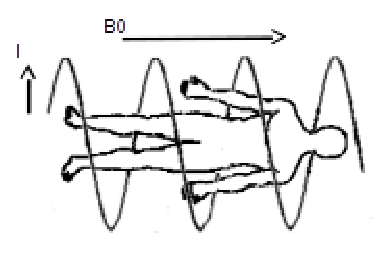
\includegraphics[width=0.7\textwidth]{seguridad_bcero}
   \caption{Campo Magnético creado por un conductor de forma helicoide: I representa la corriente continua que circula a lo largo de conductor y B0 representa el campo magnético generado. }
 \label{fig:seguridad_bcero}
 \end{figg}
\end{figure}




El valor de \Bzero es expresado en unidades de inducción magnética que, para RM, son el Tesla (T) y el Gauss. Un campo magnético es una magnitud vectorial con una dirección (como se mencionó anteriormente), que circula alrededor de un sistema de corriente que lo produce y cuya magnitud decrementa con el cuadrado de la distancia del sistema de corriente. Cuando un material que contiene protones de Hidrógeno es colocado dentro de un campo magnético, el momento magnético de estos comienza a precesar alrededor del campo estático. La frecuencia de precesión depende de la densidad de flujo magnético local y el núcleo en cuestión  (para el caso del protón del núcleo de Hidrógeno presente en la molécula de agua, la frecuencia de resonancia es de 42.57 MHz/T, conocida como la frecuencia de Larmour). Entendiendo el mecanismo mediante el cual ocurre el fenómeno de RM,  ahora se pueden abordar los efectos sobre los sistemas biológicos producidos por la exposición a campos magnéticos.

\subsection{Efectos biológicos}

La introducción de la tecnología de RM a los contextos clínicos desde 1980 ha provocado un incremento sustancial en la exposición del hombre a potentes campos magnéticos estáticos \cite{Schenck_2000}. La mayoría de los sistemas de RM en uso, hoy en día, operan con campos magnéticos estáticos que van desde 0.2 hasta 3 T. En el marco de la investigación, se utilizan campos magnéticos excepcionalmente potentes de hasta 8 T. Según las últimas directrices de la \emph{Food and Drug Administration} (FDA), la utilización clínica de campos magnéticos estáticos de 8.0 T se considera de ``bajo riesgo'' para los pacientes; sin embargo, la exposición de los sujetos de investigación a campos mayores a 8 T requiere la aprobación de un comité de revisión institucional y el consentimiento informado de los sujetos \cite{Shellock_2000}.

Es importante evaluar los efectos fisiológicos que la exposición a la RM podría producir, tales como enlentecimiento en la velocidad de conducción nerviosa, perturbaciones en la electrofisiología normal y efectos sobre la dinámica de los fluidos \cite{Magin_Liburdy_Persson_1992,HealthProtectionAgency_2008};algunos de estos fenómenos se resumen a continuación. 

\subsubsection{Efectos sobre la velocidad de conducción nerviosa}
El argumento teórico de una posible disminución en la velocidad de conducción de los nervios por la exposición a campos magnéticos, se basa en que los campos magnéticos actúan sobre las corrientes iónicas de la misma manera que actúan sobre una carga eléctrica moviéndose en un campo: 
\begin{equation}
 F = q(\nu \cdot B_0)
 \label{eq_F}
\end{equation}
donde $q$ es la carga, $\nu$ es la velocidad y \Bzero es el campo magnético. Esta fuerza causa una distorsión que es perpendicular tanto al campo magnético como a la dirección original del movimiento iónico. Un campo magnético perpendicular a los circuitos de corriente asociados con la propagación a lo largo del nervio podría resultar en una distorsión de estos mismos circuitos y consecuentemente en una disminución de la velocidad de la corriente. De manera teórica, Wikswo y Barach (1980) \cite{Wikswo_Barach_1980} demostraron que se requiere de una potencia de 24 T para reducir la velocidad de conducción del potencial de acción en un 10\%; sin embargo, otros estudios no han reportado cambios en la conducción nerviosa en equipos de 2 a 9 T. Una posible explicación a esto es que la velocidad de conducción podría cambiar debido a la falta de un adecuado control de la temperatura, ya que un cambio de 0.2\degrees \xspace podría causar cerca del 2\% de cambio en la conducción de la velocidad.

Efectos sobre el Electrocardiograma. Un potencial eléctrico puede ser producido por un conductor en movimiento tal como el flujo sanguíneo, el pulso cardiaco o la respiración de los pulmones en un campo magnético. El potencial eléctrico inducido por este movimiento produce una señal superpuesta en el electrocardiograma normal, la cual incrementa con la fuerza del campo:
\begin{equation}
 E=\nu \cdot B_0 \cdot d
\end{equation}
para un flujo que se conduce de manera perpendicular al campo magnético, donde $E$ es el potencial eléctrico y $d$ es el diámetro del vaso. La magnitud del campo $E$ asociado a este cambio en el potencial es mucho menor que el necesario para producir una excitación eléctrica del corazón, lo que se concluye teóricamente, ya que, a 10 T, el campo $E$ en la aorta es 10 veces menor que el campo $E$ teórico necesario para una excitación eléctrica cardiaca.

\subsubsection{Efectos sobre el Electroencefalograma}
Reportes en la literatura sobre los efectos del campo magnético en las ondas cerebrales en diversos experimentos usando electrodos implantados en el cerebro de modelos animales  han reportado efectos asociados con artefactos producidos por el movimiento de los electrodos dentro del campo magnético, no así, efectos fisiológicos.

\subsubsection{Efecto de Frenado en el Flujo de Conductores} 
Considerando un tubo de sangre que fluye a una velocidad $\nu$ perpendicular al campo magnético (\Bzero) y que, como ya se mencionó, se tiene que una fuerza $F$ sobre los conductores es dada por la ecuación \ref{eq_F}:
La corriente de iones asociada con esta fuerza está relacionada a la conductividad. Esta corriente es también perpendicular al campo magnético  y al flujo; es el resultado de la interacción de esta corriente y el campo magnético estático y otra fuerza que se encuentra en dirección opuesta a la velocidad de la sangre. Sin embargo, cálculos teóricos acerca de la dinámica de este efecto, muestran que este no es significativo para producir cambios en la dinámica circulatoria en humanos. Lo cual es congruente con la ausencia de reportes de efectos significativos en humanos, con excepción de vértigos y nauseas en algunos sujetos a 4 T.

Schenck \cite{Schenck_2000,Schenck_1992} ha llevado a cabo un amplio análisis de los efectos biológicos asociados a la exposición a campos magnéticos estáticos. Con respecto a la exposición a corto plazo (por ejemplo, aquellas exposiciones asociadas con el uso clínico de los sistemas de RM), la información disponible sobre los efectos de los campos magnéticos estáticos en los tejidos biológicos es extensa \cite{Schenck_2000,Schenck_1992,Besson_Foreman_Eastwood_Smith_Ashcroft_1984}. Las investigaciones incluyen estudios sobre las alteraciones en crecimiento y morfología celular, reproducción celular y teratogenicidad, estructura del ADN y expresión genética, desarrollo pre y postnatal, permeabilidad de la barrera hemato-encefálica, actividad nerviosa, función cognitiva y conducta, dinámica cardiovascular, índices hemáticos, regulación de la temperatura, ritmos circadianos, respuesta inmune y otros procesos biológicos. En la mayoría de estos estudios, los autores concluyeron que la exposición a campos magnéticos estáticos no produce efectos biológicos nocivos importantes. Aunque ha habido algunos reportes de los efectos potencialmente perjudiciales de los campos magnéticos estáticos sobre células aisladas o de los organismos, ninguno de estos efectos se han comprobado o establecido de manera concluyente como un hecho científico. Las lesiones producidas por el uso de sistemas de RM son relativamente poco documentadas y se atribuyen principalmente a la presencia accidental o introducción de objetos ferromagnéticos al equipo de RM.

\subsubsection{Objetos ferromagnéticos}
Aparte de los posibles efectos biológicos producidos por la exposición a la RM, hay que tener siempre presentes los riesgos que conlleva esta tecnología en relación a su efecto sobre los objetos metálicos, como ya se mencionó anteriormente.  Es importante definir qué objetos pueden verse afectados por los campos magnéticos y pueden constituir un riesgo potencial al momento de utilizar esta tecnología. De acuerdo con su comportamiento al ser sometidos a campos magnéticos, las sustancias y objetos pueden clasificarse en tres categorías:
\begin{description}
 \item [Paramagnéticas] Son débilmente atraídas hacia la zona de campo magnético más intenso.
 \item [diamagnéticas] Son débilmente repelidas hacia las regiones de menor campo magnético. 
 \item [ferromagnéticas] Son fuertemente atraídas hacia la zona de campo magnético más intenso. 
\end{description}



Si el campo magnético externo es el creado en el interior de un solenoide de valor $B_0 = \mu_0 nl$, al situar dentro del solenoide una sustancia, el campo pasará a tener un valor $B_0 = \mu nl$, donde $\mu$ es la permeabilidad magnética de la sustancia. La permeabilidad de cualquier medio puede expresarse como $\mu = \mu_r \mu_0$ , donde $\mu_r$ es la permeabilidad relativa. Usualmente se define: $\mu_r = 1 + \chi_m$ , donde $\chi_m$ es la susceptibilidad magnética, una magnitud importante para caracterizar el comportamiento magnético de las sustancias.

El \textbf{diamagnetismo} es una forma muy débil de magnetismo que no es permanente y persiste sólo mientras se aplique un campo externo, este es inducido por un cambio en el movimiento orbital de los electrones debido a la aplicación de un campo magnético. La magnitud del momento magnético inducido es extremadamente pequeña y en dirección opuesta al campo aplicado, por ello, $\mu_r$ es menor que la unidad y la susceptibilidad magnética, es negativa; o sea que la magnitud del campo magnético B dentro de un sólido diamagnético es menor que en el vacío. El diamagnetismo produce una susceptibilidad magnética negativa muy débil, del orden de $\chi_m = 10^{-6}$.  Cuando un material diamagnético se coloca entre polos de un electromagneto fuerte, es atraído hacia las regiones donde el campo es débil. El diamagnetismo se encuentra en todos los materiales pero solo puede observarse cuando otros tipos de magnetismo están totalmente ausentes. Esta forma de magnetismo no tiene importancia práctica.

En el caso del \textbf{paramagnetismo} se debe considerar que para algunos materiales sólidos cada átomo posee un momento dipolar permanente en virtud de la cancelación incompleta del spin electrónico y/o de los momentos magnéticos orbitales. En ausencia de un campo magnético externo, las orientaciones de esos momentos magnéticos son al azar, tal que una pieza del material no posee magnetización macroscópica neta. Esos dipolos atómicos son libres para rotar y cuando se alinean en una dirección preferencial por rotación al aplicar un campo externo, resulta el paramagnetismo. Estos dipolos magnéticos actúan individualmente sin interacción mutua entre dipolos adyacentes. Como los dipolos se alinean con el campo externo, actúan en forma sinérgica dando lugar a una $\mu_r$ mayor que la unidad y a una susceptibilidad magnética relativamente pequeña pero positiva. El efecto del paramagnetismo desaparece cuando se elimina el campo magnético aplicado.


Para aquellos materiales que poseen un momento magnético permanente en ausencia de un campo externo y manifiestan magnetizaciones muy largas y permanentes se habla de \textbf{ferromagnetismo}, el cual es presentado por algunos metales de transición, Fe, Co, Ni y algunas tierras raras como el gadolinio (Gd). Cuando se hace incidir un campo magnético sobre una sustancia ferromagnética, se produce un desplazamiento de las paredes de los dominios, de modo que aumenta el número de aquellos cuyo momento magnético está orientado a favor del campo y disminuye el de los demás. Si el campo externo es lo suficientemente intenso, se puede producir, incluso, un giro brusco de los momentos magnéticos de los dominios en la dirección del campo, lo que aumenta la magnetización del material. El imán o material ferromagnético puede mantener durante mucho tiempo esta orientación de sus dominios, aún si desaparece el campo externo.  Estos objetos ferromagnéticos requieren de especial atención en los procedimientos de RM, ya que la forma en la que interactúan con los campos magnéticos puede convertirlos en proyectiles, produciendo severos daños en los pacientes que ingresan a los equipos de RM. Por ejemplo, pequeños objetos ferromagnéticos, como clips y pasadores para el cabello, pueden alcanzar una velocidad de 64 km/hr cuando son introducidos en un campo magnético de 1.5 T. 

Muchos de los materiales de cirugía, como pinzas, tijeras y otros implementos de acero inoxidable o sustancias ferromagnéticas, se ven atraídos por el campo magnético generado en la RM. Entre otros objetos ferromagnéticos se pueden identificar implantes, dispositivos y otros materiales colocados en algunos pacientes que producen los mismos efectos que cualquier otro objeto ferromagnético. Los principales efectos incluyen: la generación de proyectiles, deformaciones de los implantes y dispositivos por torsión de los metales, calentamiento y subsecuentes quemaduras, y artefactos en la imagen por RM. Antes de permitir el acceso de los participantes o pacientes al entorno de RM se debe realizar una selección cuidadosa para determinar la presencia de implantes, dispositivos u objetos que puedan representar peligros o riesgos. Una vez identificados, se debe decidir si es aceptable que el participante o paciente ingrese al entorno de RM o se someta a un procedimiento de RM. En los apartados siguientes se abordará con mayor detalle las reglas de compatibilidad y las restricciones en cuanto al uso de ciertos materiales.

\subsection{Campo magnético del gradiente}
Todos los sistemas de RM están equipados con un conjunto de bobinas conocido como bobinas de gradiente. La función de los gradientes es proporcionar una variación en la fuerza del campo magnético encendiendo y apagando  pulsos de gradiente entre los pulsos de excitación de radiofrecuencia. El propósito de estos gradientes es el de codificar espacialmente la información contenida en la señal de radiofrecuencia producida por la caída y relajación de los spins; sin embargo, al hacerlo, se crea un campo magnético variable en el tiempo. Esta variación del campo magnético en el tiempo puede inducir corrientes eléctricas en los circuitos biológicos y, si ésta fuese importante, podría causar excitación de las células musculares o nerviosas, fibrilaciones, aumento de osmolaridad cerebral y alteración de la remodelación ósea.

Es importante considerar que si la corriente inducida es suficiente, podría generarse un potencial de acción en los tejidos excitables. Para la estimación de la corriente inducida se debe tomar en cuenta que la densidad de corriente inducida ($J$) depende de la conductividad eléctrica del medio ($\sigma$), de las condiciones geométricas del circuito (Superficie: $S$ y Longitud del conductor: $L$), de la magnitud de la variación del campo magnético ($dB/dt$) y de la dirección del campo magnético respecto a la superficie:
\begin{equation}
  J = \sigma \cdot S/L \cdot dB/dt
\end{equation}

Si consideramos que la densidad de corriente para crear un potencial de acción en un nervio es de 300 $\mu$A/$cm^2$ \cite{Budinger_1983}, tenemos que, para obtener la magnitud de la variación del campo magnético que induciría el potencial de acción, sólo se despeja la formula considerando valores conocidos respecto a $\sigma$ y $S/L$ del conductor, dada por el radio considerando un conductor circular. De esta manera, se obtendría la magnitud del gradiente máximo. La FDA ha establecido como valores máximos aconsejables: variaciones de campo magnético del orden de los 20 T/s para pulsos mayores de 120 $\mu$s, o 200 T/s para pulsos de amplitud menor de 12 $\mu$s. Además se debe cuidar la colocación de los pacientes en las exploraciones dentro del escáner, ya que pueden formarse circuitos en el cuerpo o body loops, los cuales pueden inducir corrientes; para ello, se debe instruir al paciente para que no cruce los brazos o las piernas durante la exploración, también pueden separarse estos puntos de contacto mediante material no conductor.

Como ya se mencionó anteriormente, durante los procedimientos de RM, el gradiente de campo magnético puede estimular los nervios o los músculos mediante la inducción de campos eléctricos en los pacientes. El tema ha sido ampliamente revisado \cite{Nyenhuis_Bourland_Schaefer_1997,Bourland_Nyenhuis_Schaefer_1999}. Las interacciones entre gradiente de campo magnético y tejido biológico dependen de una variedad de factores, incluyendo la frecuencia del campo principal, la densidad de flujo máximo, la densidad media de flujo, la presencia de frecuencias armónicas, las características de forma de onda de la señal, la polaridad de la señal, la distribución de corriente en el cuerpo, las propiedades eléctricas y la sensibilidad de la membrana celular. Dos de los efectos biológicos mejor identificados en relación a los cambios de gradientes en el campo magnético son la estimulación del nervio periférico y el ruido acústico; a continuación se describirán algunas de sus características.

\subsubsection{Estimulación nerviosa periférica}
La aplicación de gradientes de campo magnético puede inducir una corriente en materiales conductores, incluyendo los nervios y el tejido muscular. La corriente inducida es mayor en los tejidos periféricos y se pueden producir sensaciones leves en la piel y contracciones musculares involuntarias. Estas sensaciones pueden escalar a sensaciones dolorosas o desagradables si se incrementa la intensidad del gradiente de campo magnético; al escanear, se pueden inducir corrientes que influyan en la función cardiaca y, en casos extremos, causen fibrilación ventricular. Los estudios llevados a cabo en los participantes durante investigación, indican que los sitios anatómicos donde se produce la estimulación de nervios periféricos por efecto de los gradientes de campo magnético, varían en función de la activación de un gradiente específico (es decir en el gradiente $x$, $y$, $z$) (Tabla \ref{tab_seguridad}). Por lo general, los sitios de estimulación del nervio periférico se han encontrado en las prominencias óseas; ya que el hueso es menos conductor que el tejido circundante, las densidades de corriente pueden aumentar en regiones estrechas de tejido entre el hueso y la piel, lo cual reduce los umbrales de estimulación nerviosa más de lo esperado. Los individuos sometidos a RM deben ser instruidos para reportar cualquier sensación al operador del escáner, para llevar a cabo la acción pertinente \cite{Kangarlu_Robitaille_2000,HealthProtectionAgency_2008}. 


\begin{table}[hbtp]
\centering
\caption{Sitios de estimulación según el gradiente aplicado (Medical College of Wisconsin 2009)}
\label{tab_seguridad}
\begin{tabular}{@{}ll@{}}
\toprule
\textbf{Sitios de Estimulación del Nervio Periférico} & \textbf{Gradiente}   \\ \midrule
Puente de la nariz                           & $x$         \\
Hombros                                      & $y$         \\
Escápula                                     & $y$,$z$     \\
Porción proximal de los brazos               & $y$         \\
Espalda alta                                 & $y$,$z$     \\
Tórax                                        & $z$         \\
Porción izquierda del tórax                  & $x$         \\
Porción derecha del tórax                    & $y$         \\
Xifoides                                     & $z$         \\
Abdomen                                      & $z$         \\
Cresta iliaca                                & $x$,$y$,$z$ \\
Espalda baja                                 & $x$, $z$    \\
Cadera                                       & $y$         \\
Nalgas                                       & $x$         \\
Muslo izquierdo                              & $x$         \\
Manos                                        & $y$         \\ \bottomrule
\end{tabular}
\end{table}


\subsection{Ruido acústico}
Otra de las consecuencias del encendido y apagado de los gradientes es que, en presencia de un campo magnético estático, las corrientes en las bobinas de gradiente generan fuerzas que implican vibraciones con sus consecuentes ruidos, los cuales pueden llegar a ser de alta intensidad \cite{Shellock_2000}. La frecuencia y la tonalidad dependen de muchos factores, entre ellos el diseño de aparato y la secuencia utilizada \cite{Miyati_Banno_Fujita_Mase_Narita_Imazawa_Ohba_1999}. Los problemas asociados con el ruido acústico para los pacientes o participantes y el personal incluyen: simple irritación, dificultades en la comunicación verbal, incremento de la ansiedad, pérdida de audición temporal y, posiblemente, deterioro permanente de la audición \cite{McJuryPhD_ShellockPhD_2000,Hurwitz_Lane_Bell_Brant-Zawadzki_1989}. El ruido acústico puede representar un peligro, en particular para grupos específicos de pacientes que están en mayor riesgo. Los pacientes con trastornos psiquiátricos, ancianos, y niños pueden presentar sensaciones de confusión o una mayor experiencia de ansiedad \cite{Quirk_Letendre_Ciottone_Lingley}. Los pacientes sedados pueden experimentar malestar general debido a los altos niveles de ruido. Ciertos medicamentos, conocidos por aumentar la sensibilidad auditiva, pueden producir mayores sensaciones de malestar \cite{Laurell_1992}. Los recién nacidos con inmadurez en el desarrollo anatómico pueden tener una reacción mayor ante el ruido acústico \cite{Philbin_Taber_Hayman_1996}.

Las variaciones del ruido acústico relacionadas con RM ocurren cuando se realizan modificaciones en la salida de gradiente (incremento del tiempo o de la amplitud) y también se asocia con los distintos parámetros de RM \cite{McJuryPhD_ShellockPhD_2000,Counter_2000,Cho_Park_Kim_Chung_Chung_Chung_Moon_Yi_Sin_Wong_1997}. El incremento en los niveles de ruido, tono y frecuencia se debe principalmente a una reducción en los tiempos de repetición y de eco. Las características físicas del equipo (especialmente la presencia o ausencia de aislamiento especial del sonido y el material con el que se construyeron las bobinas de gradiente y estructuras de apoyo) también influyen en la transmisión de ruido acústico y su percepción por los pacientes o participantes \cite{Philbin_Taber_Hayman_1996}.

La presencia y tamaño del paciente también afecta el nivel de ruido acústico. Se ha informado un incremento en el ruido acústico cuando el paciente o participante se encuentra dentro del escáner, este fenómeno se puede deber a la doble presión que se genera por la cercanía de un objeto, de tal manera que las ondas del sonido se reflejan y sincronizan su fase. Las características del ruido también presentan dependencia del espacio, por ejemplo, se ha descubierto que los niveles varían hasta en 10 dB en función de la posición del paciente a lo largo del diámetro del magneto \cite{Hedeen_Edelstein_1997}.

Los niveles de ruido relacionados con la RM han sido medidos durante diferentes secuencias de pulsos para sistemas de RM que van desde los 0.2 hasta los 4.7 T \cite{Counter_2000,Shellock_2000}. Estudios recientes han demostrado que las secuencias de pulsos de gradiente de eco rápidos, spin-eco y secuencias eco-planares producen un mayor nivel de ruido \cite{Price_DeWilde_Papadaki_Curran_Kitney_2001,McJuryPhD_ShellockPhD_2000}. La FDA indica que los límites permisibles de ruido acústico relacionado con RM se encuentran por debajo del nivel establecido según las regulaciones federales o los estándares propuestos por otras organizaciones. Si el ruido acústico no se encuentra por debajo de estos niveles, el fabricante debe recomendar las medidas pertinentes para la reducción del ruido percibido por el individuo. El pico de ruido acústico de 140 dB es el límite superior; sin embargo, las instrucciones para el uso del equipo deben indicar al operador que se proporcione protección para los oídos a los pacientes o participantes cuando se opere en niveles por arriba de los 99 dB \cite{Shellock_2000}.

En general, si se siguen las reglas establecidas por los organismos reguladores para el control del ruido acústico relacionado con la RM, los procedimientos no suelen ser problemáticos debido a los períodos exposición de tiempo relativamente cortos.




\section{Medidas de prevención de accidentes}

\subsection{Evaluación Clínica}
Los individuos que van a ser expuestos a entornos de RM, ya sea con fines clínicos o de investigación, deben ser evaluados para conocer su condición médica y determinar si existen riesgos para que puedan ingresar a RM; debe considerarse que no tengan problemas que puedan impedir que se mantengan acostados o permanezcan quietos durante largos períodos de tiempo. Aquellos pacientes que requieren mantenerse durante medicación continua a través de dispositivos externos o internos deben ser excluidos como candidatos a estudios de RM; aquellos quienes no entienden las instrucciones o no pueden cooperar con el personal encargado del equipo de RM para asegurar el éxito del estudio deben ser considerados cuidadosamente. Los individuos que portan algún dispositivo o implemento médico de manera permanente o cualquier otro objeto ferromagnético o con características ferromagnéticas deben ser excluidos o evaluados cuidadosamente. En cualquier caso, todos los individuos deben ser evaluados muy rigurosamente para garantizar la seguridad de los implicados y la efectividad del estudio. A continuación se describen algunos procedimientos y aspectos a tomar en cuenta a la hora de considerar a un candidato para RM.

\subsubsection{Formulario de evaluación preliminar}
Antes del ingreso del paciente a la sala de exploración de RM, se debe llevar a cabo una serie de pasos que garanticen la seguridad del mismo; estos se pueden facilitar a través del uso de un cuestionario de escrutinio para detectar riesgos de exploración del paciente en RM, en las Figuras \ref{fig:seguridad_formularioA} y \ref{fig:seguridad_formularioB} se muestra un ejemplo de la información que debe contener dicho cuestionario.



\begin{figure}[htb]
\begin{figg}
   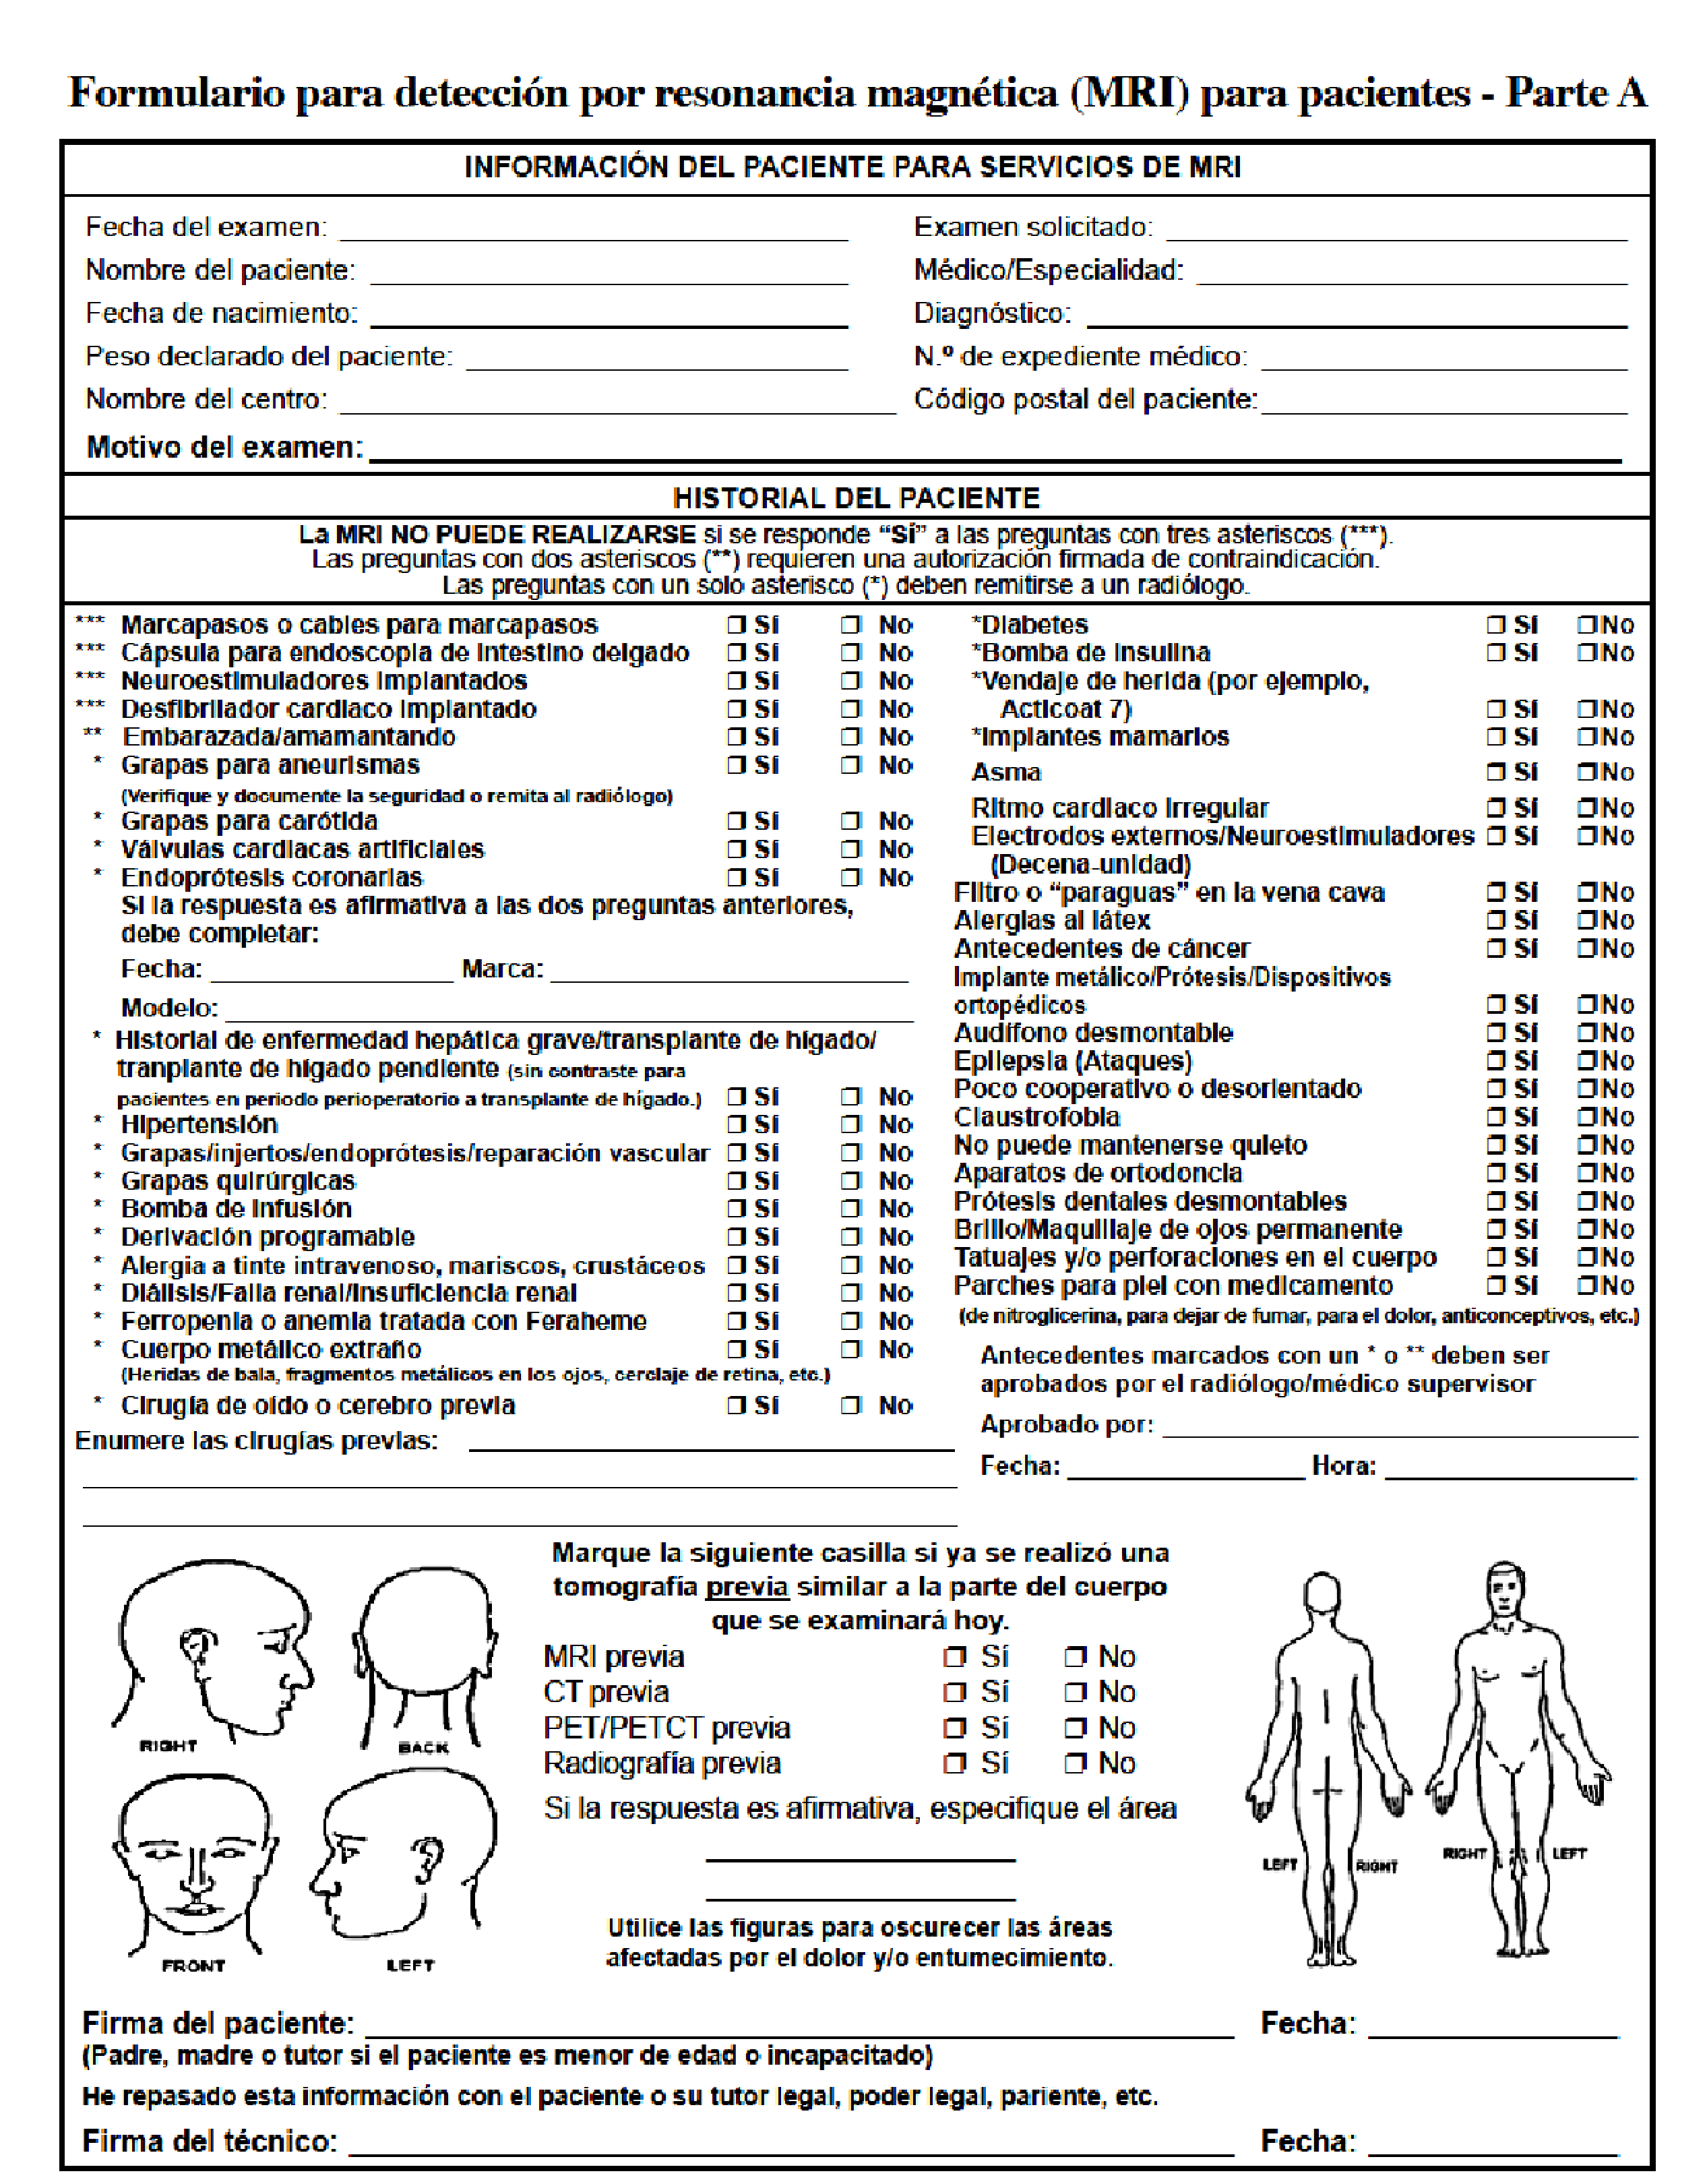
\includegraphics[width=0.7\textwidth]{seguridad_formularioA}
   \caption{Formulario de detección por Resonancia Magnética para pacientes (anverso). Tomado de Day Kimbal Healthcare. }
 \label{fig:seguridad_formularioA}
 \end{figg}
\end{figure}

\begin{figure}[htb]
\begin{figg}
   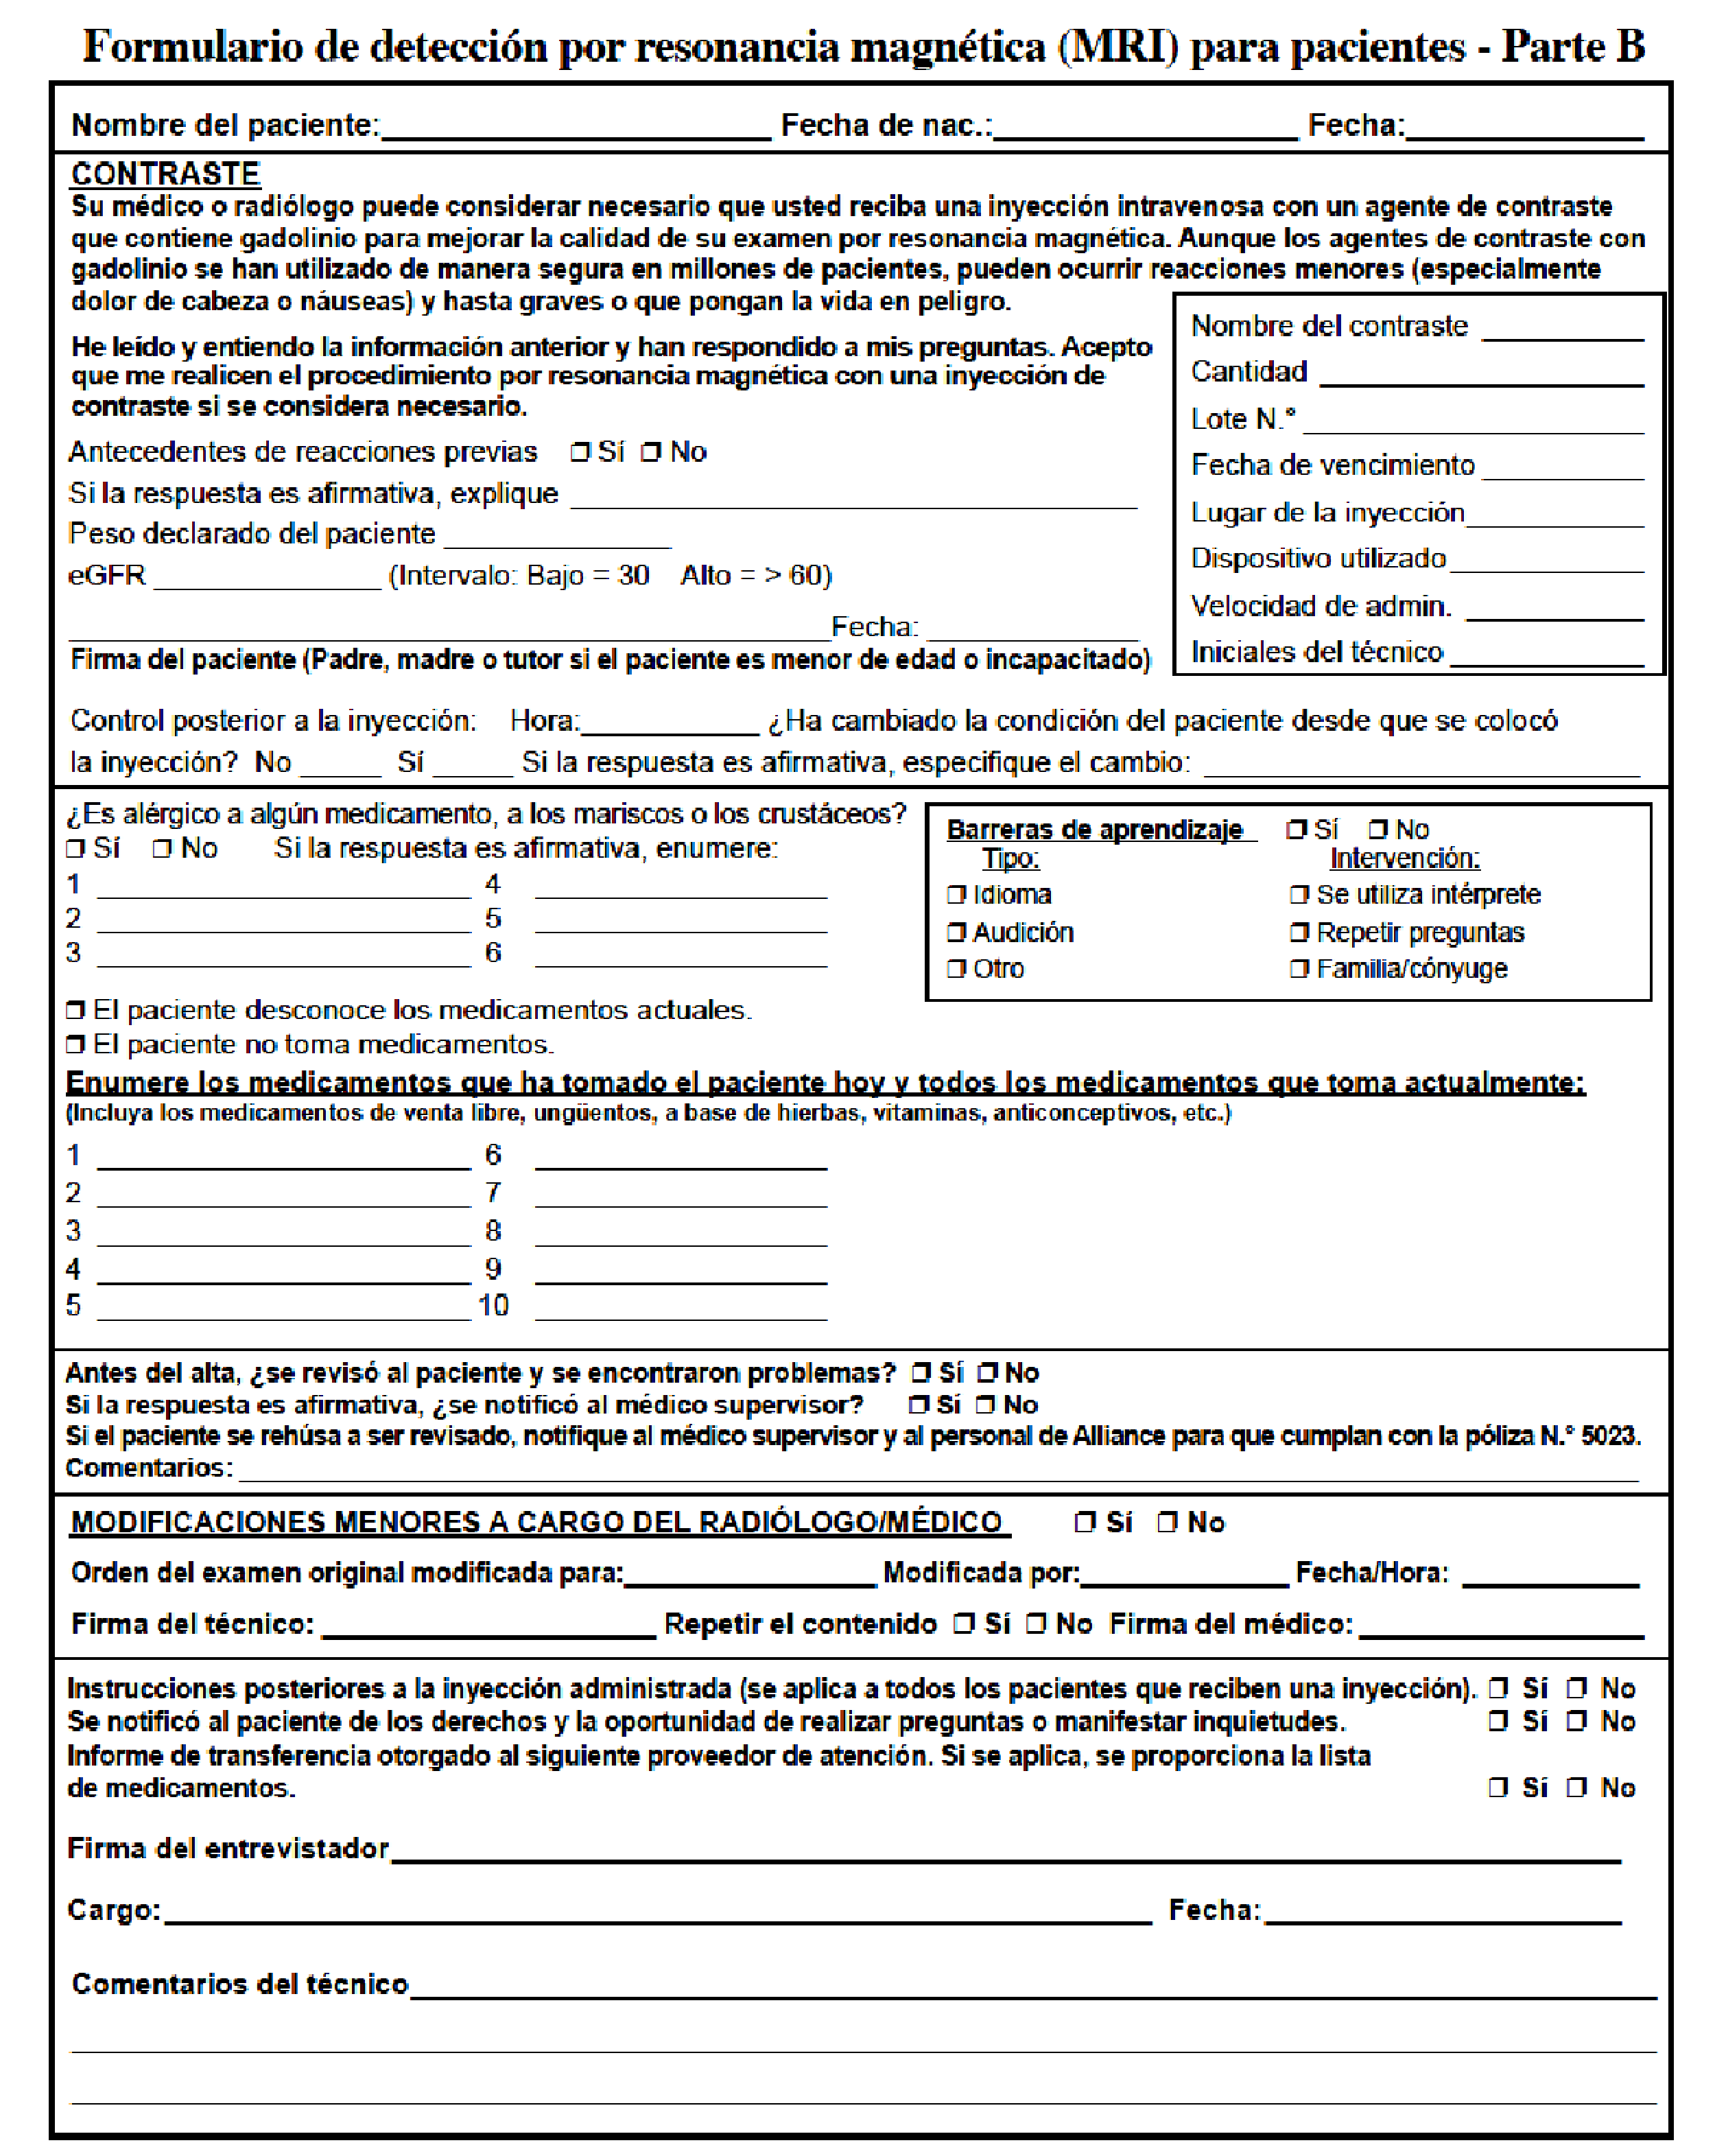
\includegraphics[width=0.7\textwidth]{seguridad_formularioB}
   \caption{Formulario de detección por Resonancia Magnética para pacientes (reverso). Tomado de Day Kimbal Healthcare. }
 \label{fig:seguridad_formularioB}
 \end{figg}
\end{figure}



Los pasos siguientes, que incluyen el uso del formulario, deben de llevarse a cabo antes de iniciar el estudio dentro de la sala de RM: 

\begin{enumerate}
\item Interrogar al paciente sobre posibles implantes metálicos internos y externos al recibirle y antes de entrar en la sala exploración, estableciendo, así, diferentes filtros de seguridad.
\item En caso de duda sobre la compatibilidad de un implante con el equipo de RM, realizar la exploración sólo hasta tener la documentación necesaria sobre el objeto.
\item Retirar audífonos y dentaduras postizas.
\item Retirar materiales metálicos que lleve el paciente externamente (reloj, cadenas, anillos, etc.) y tener la misma conducta para el personal médico, acompañantes, y todo aquel que vaya ingresar a la sala del escáner.
\item Atención al uso de aparatos de reanimación como desfibriladores, tanques de oxígeno, etc., no utilizarlos nunca dentro de la sala de exploración (salvo que exista compatibilidad con RM).
\item Verificar que los pacientes no lleven maquillaje, en caso de que así sea retirárselo. Se debe prestar especial atención a pacientes con tatuajes o con maquillaje permanente, dando instrucciones al individuo para que avise del calentamiento de esa zona y, en el caso de que esto sucediese, retirarlo inmediatamente.
\end{enumerate}



\subsubsection{Compatibilidad con RM}
En 1997, la FDA  y el \emph{Center for Devices and Radiological Health}, crearon dos categorías para el uso de objetos e implementos en los entornos de RM, estos son: RM Seguro y RM Compatible. RM Seguro: aquellos objetos, implantes o dispositivos que cuando son usados en entornos de RM han demostrado no  representar un riesgo adicional para el participante o paciente, aunque pueden afectar la calidad de los datos adquiridos. RM Compatible: aquellos objetos que, aparte de haberse comprobado que son seguros en entornos de RM, cuando son usados tampoco afectan la calidad de los datos que se adquieren. Tanto en los materiales considerados seguros como los materiales considerados compatibles debe especificarse las condiciones en que el material ha sido probado, ya que un material puede considerarse seguro o compatible bajo determinadas condiciones y no en otras condiciones. Sin embargo, estos términos han sido debatidos ya que existe cierta ambigüedad en la práctica. 

Para tener una mayor claridad y certeza de la seguridad de los individuos en entornos de RM la \emph{American Society for Testing and Materials} (ASTM) introdujo en 2005 tres categorías: RM Seguro, RM Condicional y RM No seguro. \textbf{RM Seguro} es aquel material que no representa ningún peligro conocido en todos los entornos de RM. Entre los materiales se incluyen no conductores, objetos no metálicos y no magnéticos. \textbf{RM Condicional} son aquellos objetos en los que no ha sido demostrada su peligrosidad en entornos de RM bajo condiciones específicas, por ello se deben definir y considerar las condiciones del campo magnético para determinar su seguridad. \textbf{RM No seguro} son aquellos objetos cuya peligrosidad es conocida en todos los entornos de RM, como son los objetos ferromagnéticos (Figura \ref{fig:seguridad_simbolos}).



\begin{figure}[htb]
\begin{figg}
   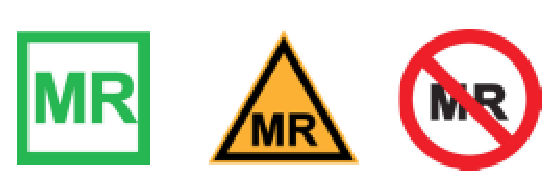
\includegraphics[width=0.7\textwidth]{seguridad_simbolos}
   \caption{Rótulos indicativos de la compatibilidad de los materiales en entornos magnéticos; de izquierda a derecha RM seguro, RM condicional y RM no-seguro.}
 \label{fig:seguridad_simbolos}
 \end{figg}
\end{figure}






Todo el equipo, usado tanto para fines de investigación como clínicos dentro de entornos de RM incluyendo proyectores, estimuladores y demás aparatos, debe ser probado previamente para verificar su seguridad en espacios magnéticos antes de entrar a alguno. Es responsabilidad del técnico o investigador, nunca tener equipo dentro de la habitación de RM sin haberlo probado previamente para verificar su atracción magnética; se recomienda tener a la mano, fuera del área de RM, un magneto para verificar que los objetos que se introducen al entorno no sean ferromagnéticos. Del mismo modo, se debe tener cuidado en hacer un minucioso escrutinio del participante o paciente para verificar que se encuentra en condiciones de ingresar a las sala de RM. El equipo que opera en entornos de RM debe ser continuamente monitoreado para verificar que no produzca distorsiones o interferencias con las imágenes o la adquisición de datos.  

El equipo seguro para RM  es desarrollado para fuerzas de campo magnético específico y configuraciones de RM específicas, por lo tanto, el equipo que funciona de manera adecuada dentro de una sala de RM no necesariamente operará en otra sala. Asimismo, se deben llevar a cabo rutinas de inspección y mantenimiento del equipo para verificar que siempre funcione correctamente. Rupturas o mal funcionamiento del equipo deben ser identificados y reportados por el operador del equipo.

\section{Emergencias}
En caso de emergencia, se deben garantizar procedimientos ordenados y adecuados que maximicen la seguridad tanto de pacientes y participantes como del personal de RM. Es primordial que exista comunicación constante entre el paciente o participante que se encuentra dentro del escáner de RM y el operador del mismo; para ello es esencial dar instrucciones claras y precisas para que el paciente o participante informe al operador del equipo de cualquier dificultad mientras se está llevando a cabo el estudio; con esta finalidad, los equipos modernos cuentan con un sistema de intercomunicación a través de micrófonos y altavoces, lo que facilita la comunicación. Durante los momentos de tranquilidad del estudio, el operador del escáner debe mantener contacto verbal con el paciente o participante. En caso de que el individuo no responda a los cuestionamientos o indicaciones del operador del escáner, se debe verificar inmediatamente que este se encuentre bien. 

En caso de que el paciente o participante presente una emergencia médica o lesión durante la realización del estudio, debe ser asistido inmediatamente fuera de la sala del escáner, para ello se debe designar un sitio donde este procedimiento se pueda llevar a cabo. Actualmente se cuenta con equipos que poseen camillas removibles que permiten realizar la maniobra con mayor facilidad en caso de emergencia; el mecanismo consiste en accionar unas palancas que separan la camilla del escáner y, de este modo, se puede retirar al individuo de la sala de RM y realizar la asistencia pertinente; en caso de no contar con este sistema, se requiere que se encuentre el personal necesario, así como el material y camillas requeridas para poder retirar al individuo en el menor tiempo posible y del modo más efectivo. En caso de que una emergencia se suscite, es importante mantener informado al encargado principal y al comité de seguridad de la unidad.

Si la emergencia se suscita debido a una falla o mal funcionamiento del equipo que pueda producir alguna lesión o daño al individuo, por ejemplo algún cortocircuito en el equipo o fuego, el operador debe realizar inmediatamente un paro de emergencia del equipo, accionando el interruptor de apagado o \emph{quench}. Si la emergencia está relacionada con la introducción de un objeto ferromagnético al escáner, se debe considerar, antes de realizar el paro de emergencia, si la situación es realmente mortal o puede producir daños severos al individuo, y, si es así, se debe llevar a cabo el paro de emergencia del equipo por el personal autorizado para ello. Este sistema generalmente debe estar colocado a la vista del personal y con fácil acceso. En caso de que la dificultad con el equipo no represente daño mortal o severo al individuo, se debe informar a los asistentes y decidir el modo más óptimo para liberar al sujeto y llevarlo fuera del campo magnético. En caso de que se requiera llevar a cabo el paro de emergencia, al accionar el interruptor, inmediatamente ocurrirá un \emph{quench} o liberación del helio liquido en forma gaseosa contenido en los compartimentos alrededor de los superconductores del equipo que permite mantener bajas temperaturas, esto, a su vez, significará una pérdida o decremento significativo del campo magnético. El paro de emergencia sólo debe ser accionado por personal autorizado y en caso de emergencia grave que pudiera implicar lesiones severas o muerte en el individuo. La pérdida repentina del campo magnético por el apagado y enfriamiento del equipo puede generar desechos y congelación dentro de la habitación y posibles dificultades para respirar; además, está perdida rápida de temperatura podría dañar el magneto o los componentes del equipo, lo que implica un costo considerable, es por ello importante realizarlo solo en caso de real emergencia. 

Para garantizar la seguridad y disminuir los posibles riesgos en el uso de equipos de RM, se recomienda llevar a cabo una serie de medidas de seguridad generales:
\begin{itemize}
 \item Implementación de cuestionarios para seleccionar a los sujetos candidatos a participar en estudios de RM libres de objetos metálicos e implantes sensibles al electromagnetismo, estableciendo sucesivos filtros de seguridad que garanticen este paso.
 \item Procurar que el paciente o participante ingrese a la sala de exploración en ropa interior y cubierto con una bata. 
 \item Verificar que el material paraclínico de uso cotidiano (silla de ruedas, camillas, pies del suelo, etc.) sea seguro para su uso en entornos de RM.
 \item Mantener señalamientos visibles de seguridad dentro y fuera de la sala exploración (Figura \ref{fig:seguridad_prohibidos}).
 \item Verificar que los interruptores de emergencia estén siempre visibles y de fácil acceso para el operador del equipo.
 \item Mantener en buen funcionamiento el sistema para la comunicación con el paciente durante la exploración.
 \item  Contar con el equipo médico y espacio necesario para la asistencia del participante en caso de emergencia.
\item  Capacitación constante del personal acerca del correcto uso y manejo del equipo así como procedimientos de emergencia y asistencia al participante o paciente. 
\end{itemize}



\begin{figure}[htb]
\begin{figg}
   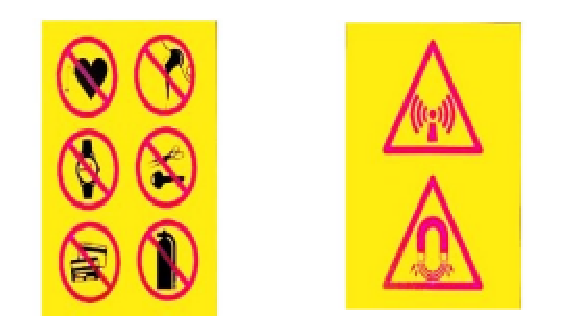
\includegraphics[width=0.7\textwidth]{seguridad_prohibidos}
   \caption{Señalamientos de seguridad para entornos de Resonancia Magnética: a) de izquierda a derecha y de arriba hacia abajo \textsc{No introducir marcapasos}, \textsc{Implantes}, \textsc{Relojes}, \textsc{Objetos ferromagnéticos}, \textsc{Tarjetas con banda magnética} y \textsc{Extintores}; b) de arriba hacia abajo, \textsc{Precaución: Radiofrecuencia} y \textsc{Magnetización}.}
 \label{fig:seguridad_prohibidos}
 \end{figg}
\end{figure}




\chapter{Espectroscopía}
\chapterprecis{\noindent Pau Marco Manclus\\Instituto de Neurobiología\\UNAM, Campus Juriquilla}
\label{chapter_espectro}

La espectroscopía es una técnica de análisis utilizada para determinar los componentes de una mezcla. A grandes rasgos se basa en el diferente comportamiento de los compuestos al absorber energía y volver a su estado natural al liberar la energía absorbida.
Dependiendo de la fuente energética para excitar los átomos de la materia podemos distinguir entre 4 clases de espectroscopía:

\begin{itemize}
 \item Espectroscopía de masas
 \item Espectroscopía de luz Ultravioleta-visible
 \item Espectroscopía de luz Infrarroja
 \item Espectroscopía de Resonancia Magnética Nuclear
\end{itemize}


En este capítulo nos centraremos en la espectroscopía de Resonancia Magnética  Nuclear (RMN). Esta técnica toma provecho de las propiedades del spin de los protones (de ahí su nombre), es la técnica más utilizada para la detección de moléculas orgánicas, y a pesar de que la espectroscopía se puede basar en diferentes átomos, la más utilizada es la espectroscopía de H, dado que su núcleo es un solo protón y este elemento se encuentra en gran proporción en componentes orgánicos y  presentes en el cuerpo.

A pesar de la gran popularidad actual de las técnicas de imagen por resonancia magnética (iRMN),  el uso de la resonancia magnética vino de la mano de la espectroscopía. La técnica de espectroscopía por RMN, a pesar de necesitar muestras mayores que las otras técnicas de espectroscopía, cuenta con la importante ventaja de ser  una técnica no destructiva, siendo posible que se desarrollase posteriormente la espectroscopía por RMN in vivo.

La espectroscopía RMN se basa en los mismos principios físicos implicados en la obtención de iRMN. En condiciones naturales los protones H presentan un spin que les concede un campo magnético propio, en presencia de un campo magnético externo, estos se pueden presentar de dos modos:
\begin{itemize}
 \item En su estado de menor energía. Alineado con el campo magnético externo (spin \nicefrac[]{1}{2}).
 \item En su estado de mayor energía. Opuesto al campo magnético externo (spin -\nicefrac[]{1}{2}).
\end{itemize}



La diferencia de energía entre estos dos estados es dependiente de la fuerza del campo magnético externo (B0) y es siempre muy pequeña. Los dos estados de spin son igualmente energéticos cuando el campo magnético externo es cero, no obstante la diferencia energética se incrementa a mayor fuerza del campo magnético externo.

\begin{figure}[htb]
 \begin{figg}
   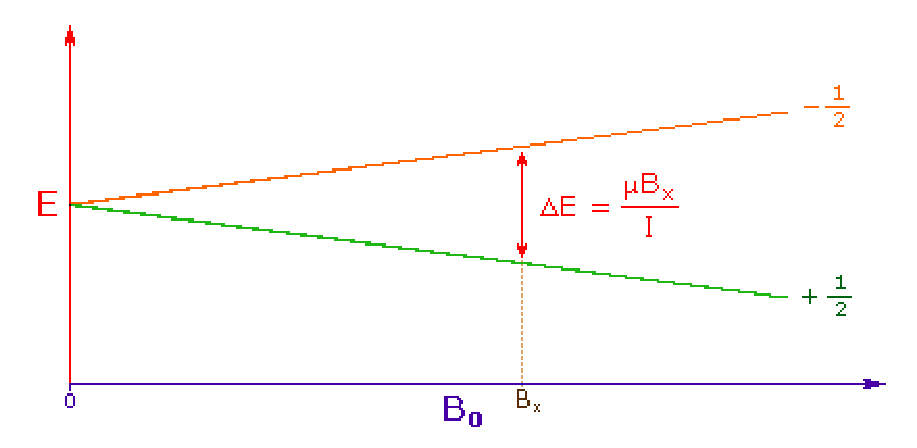
\includegraphics[width=0.7\textwidth]{espectro_deltaE}
   \caption{En el gráfico se muestra como aumentan la diferencia energética entre los dos estados de spin posible con el aumento del campo magnético \Bzero.}
 \label{fig:espectro_deltaE}
 \end{figg}
\end{figure}
 


Es por este fenómeno por el cual las técnicas de resonancia magnética requieren de potentes imanes con los que generar un fuerte campo magnético. La unidad para medir la fuerza del campo magnético del S.I. es el Tesla (T). 

En las técnicas actuales de espectroscopía se utiliza campos magnéticos de entre 1 y 20 T, pero a pesar de estos potentes campos magnéticos la diferencia entre los estados de spin es muy pequeña  (<0.1 cal/mol). 
La irradiación de una muestra con un pulso de radiofrecuencia (RF) que corresponda exactamente con la diferencia energética entre spines provocará el paso de la forma menos energética, \nicefrac[]{1}{2}, a la más energética, -\nicefrac[]{1}{2}. La diferencia entre los dos estados de spin es proporcional al momento magnético ($\mu$), siendo para H $\mu$ = 2.7927 magnetones nucleares.

Todos protones (H) tienen el  mismo momento magnético por tanto esperaríamos que todos nos dieran la misma señal. Pero de hecho, distintos protones se pueden comportar de forma distinta bajo las mismas condiciones del pulso de RF y magnetismo, cosa que nos permite discriminar entre ellos y da sentido a esta técnica analítica.

Cuando ponemos una muestra en el resonador, esta no está compuesta puramente de protones (H). Los ``protones'' que medimos se encuentran rodeados por electrones, que forman uniones de tipo covalente e iónicas, formando parte de moléculas. Los electrones son partículas cargadas negativamente, y por ello se mueven en respuesta al campo magnético externo aplicado (\Bzero) y generan un campo magnético secundario opuesto. Este campo magnético secundario opuesto amortigua el efecto del campo magnético externo sobre el núcleo. Es por ello que debemos tener en cuenta que el campo magnético efectivo (el que el núcleo ``siente'') será menor que le \Bzero, y que la pérdida de magnitud se debe al corrimiento químico ($\sigma$), el cual trataremos más adelante. 

\begin{equation}
 B = B_0 (1-\sigma)
\end{equation}

La densidad electrónica alrededor de cada átomo de una molécula varía con el tipo de núcleo y los enlaces que forma con otros átomos. El campo magnético opuesto de cada núcleo será diferente.



\begin{figure}[htb]
 \begin{figg}
   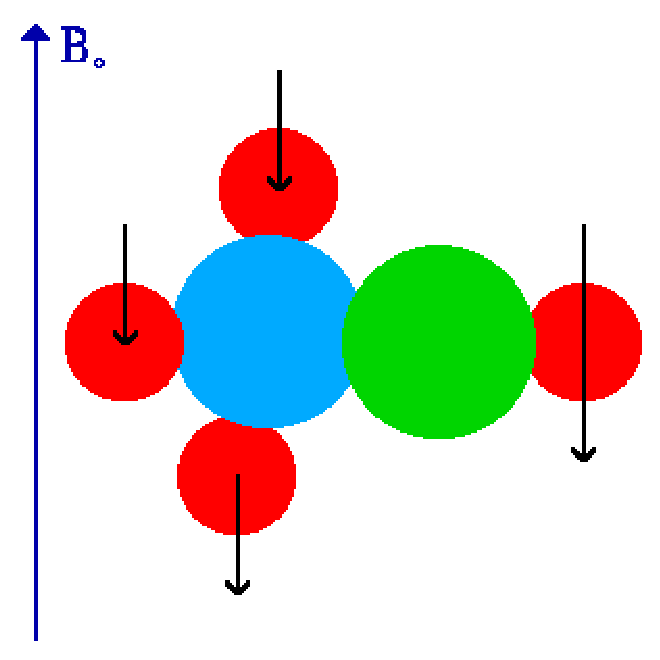
\includegraphics[width=0.7\textwidth]{espectro_metanol}
   \caption{En la imagen podemos observar una molécula de metanol en un campo magnético, \Bzero. En ella se aprecia como el H (en rojo) unido al átomo de oxigeno (O) (en verde) presenta un campo magnético opuesto mayor al de los H unidos al átomo de Carbono (C) (en azul).}
 \label{fig:espectro_metanol}
 \end{figg}
\end{figure}




La diferencia entre las frecuencias de resonancia de los protones depende del B0 (a mayor B0, mayor diferencia), esto hace que las diferencias de frecuencia no se puedan comparar con espectrofotómetros de diferentes teslajes (o incluso entre equipos distintos si consideramos que los imanes no serán exactamente iguales). 
Con la intención de resolver este problema se utiliza el corrimiento químico $\omega$. El corrimiento químico de un núcleo es la diferencia entre la frecuencia de resonancia de un núcleo y su estándar, relativo a un estándar:
\begin{equation}
 \omega = (\nu - \nu_{ref}) / \nu_{ref}
\end{equation}

Al igual que en imagen por RMN, la señal requiere la transformada de Fourier para distinguir entre los componentes de la mezcla (y sus respectivas señales). Dado que las diferencias de frecuencias son mínimas, el numerador se expresa en Hz, siendo el denominador expresado en MHz. Esto lleva a un ratio sin unidades $1/1x10^6$ (uno entre 1 millón), por lo que se expresa en unidades de ``partes por millón'' (ppm).

En espectroscopía de RMN usualmente se toma el compuesto tetrametilsilano, $Si(CH_3)_4$, (TMS), como valor de referencia; ya que es un compuesto químicamente inerte, puede ser fácilmente extraído de la mezcla y presenta una sola señal de RMN aguda (todos sus H presentan las mismas uniones) que  no interfiere con la resonancia de otros componentes orgánicos. Todos los protones (H) del TMS tienen el mismo patrón de uniones, por tanto darán todos la misma señal. Esta señal nos marcara el 0 en la escala de unidades de ppm para comparar con otros compuestos. 



\begin{figure}[htb]
 \begin{figg}
   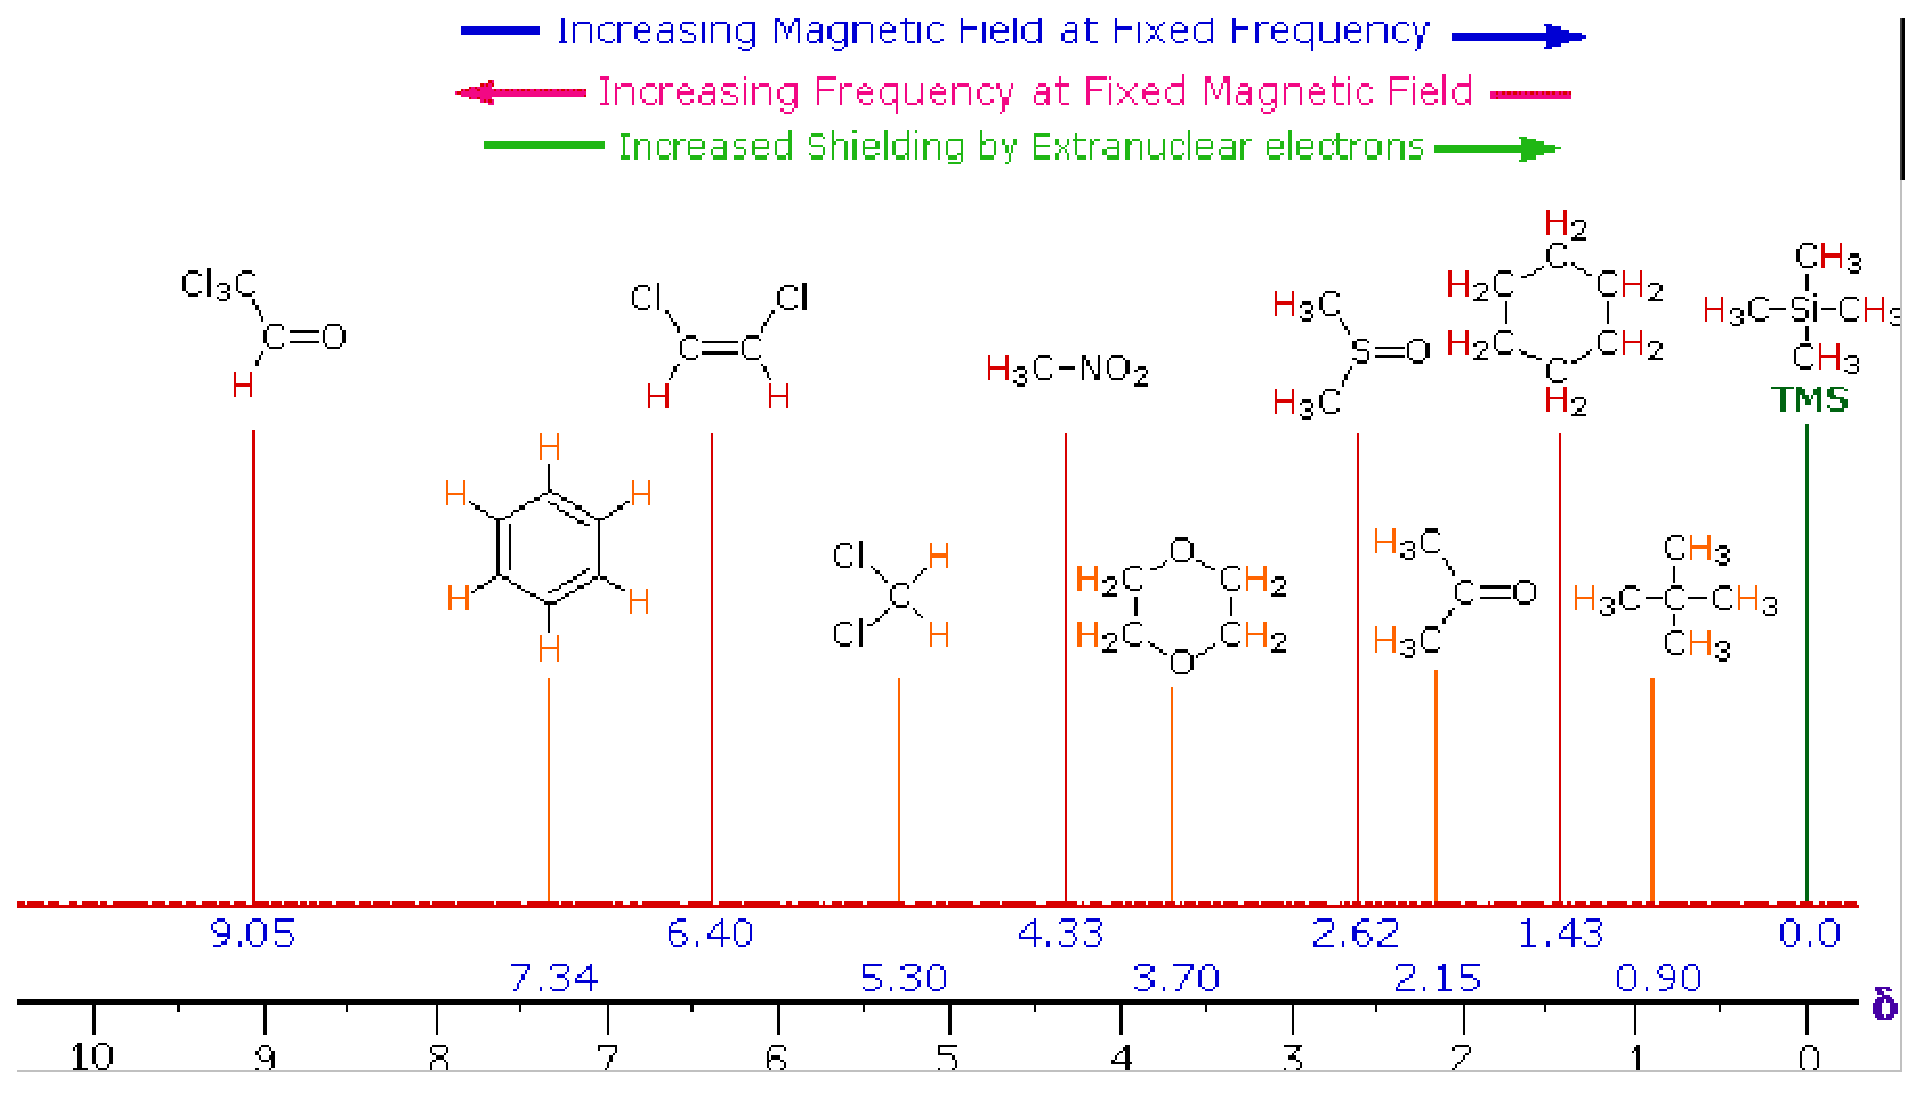
\includegraphics[width=\textwidth]{espectro_espectro}
   \caption{Falta pie de figura.}
 \label{fig:espectro_espectro}
 \end{figg}
\end{figure}


Como se mencionó anteriormente aquellos compuestos en que todos su H son estructuralmente equivalentes (mismo tipo de uniones con el mismo tipo de átomos) presentan una sola señal aguda de RMN. Por otro lado cuando esta condición no se cumpla, recibiremos una señal distinta por cada radical en el que esté involucrado un átomo de H. Dado que la técnica es incapaz de distinguir H equivalentes, la magnitud de la señal de RMN (representada en el eje de la y) es proporcional a la concentración molar de dichos protones en la muestra. Es decir a mayor intensidad de la señal, mayor será el número de H con la misma sigma y por tanto unidos al mismo tipo de átomos. (En realidad no solo está implicada la intensidad en el cálculo, este se consigue con el área que ocupa la curva de la señal).  Sin embargo, estos radicales en los que los H forman parte, no se encuentran en el vacío, y también sufren interacciones entre los H presentes en los otros radicales.
Estas interacciones tienen efecto en el espectro de RMN. Si la distancia entre núcleos no-equivalentes es menor  o igual a la longitud de 3 uniones, el efecto es observable. Este efecto se llama emparejamiento spin-spin  o emparejamiento J. En el caso de los protones con spin \nicefrac[]{1}{2} , como el H, el emparejamiento J viene determinado por:

\begin{enumerate}
 \item Los núcleos que tiene el mismo corrimiento químico (isocrónicos) no exhiben separación de spines. Pueden estar emparejados, pero la separación no puede ser observada directamente.
 \item La magnitud de la separación de spin observada  depende de varios factores y viene dado por la constante de emparejamiento J (en Hz). J es la misma para ambos compañeros de interacción de separación de spin y es independiente de la fuerza del campo magnético externo.
 \item Los núcleos separados por 3 o menos uniones tendrán usualmente spins emparejados y mostraran separación de spin mutua (misma J), demostrando que tienen diferente corrimiento químico.
 \item El patrón de separación de un núcleo dado puede ser predecida por la regla del n+1, donde n es el número de vecinos spin emparejados con la misma J. Si hay 2 núcleos vecinos, con spin emparejado, la señal observada será un triplete (2+1=3); si hay 3, se observará un cuarteto (3+1=4); etc.
\end{enumerate}


Si el núcleo tiene emparejamiento de spin con dos o más grupos de núcleos vecinos por diferentes valores de J, entonces la regla de n+1 ya no predecirá por completo el patrón de separación


\begin{figure}[htb]
 \begin{figg}
   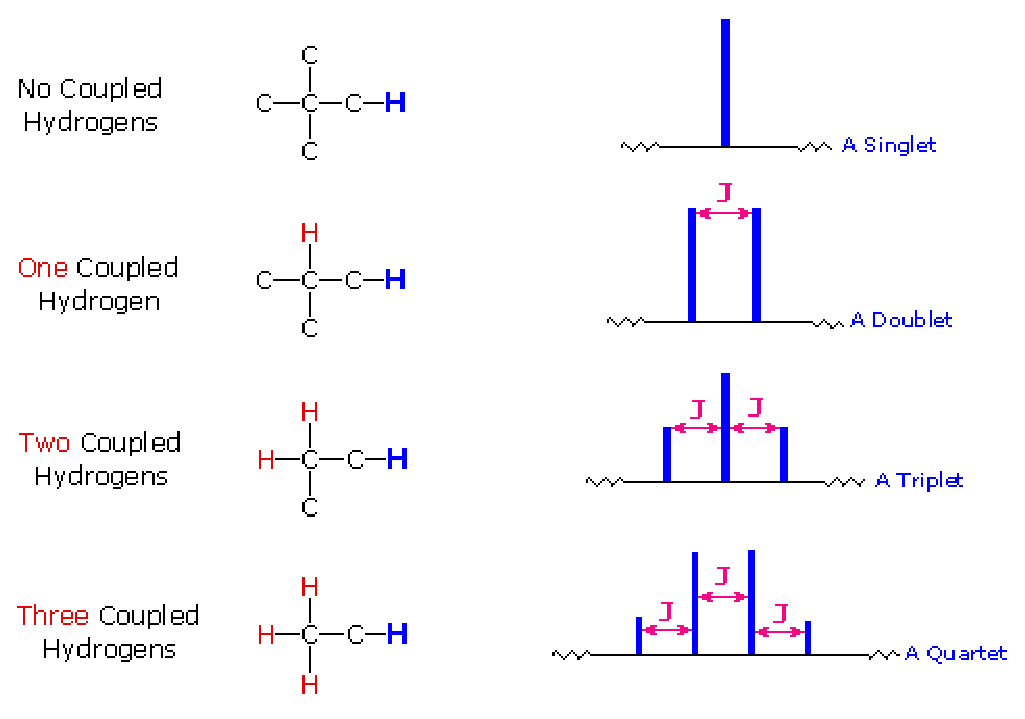
\includegraphics[width=0.7\textwidth]{espectro_coupling}
   \caption{Representación esquemática de los espectros referentes al H en azul. Cada uno de los H en rojo representa un núcleo emparejado con el H azul (con la misma J).}
 \label{fig:espectro_coupling}
 \end{figg}
\end{figure}







\begin{figure}[htb]
 \begin{figg}
   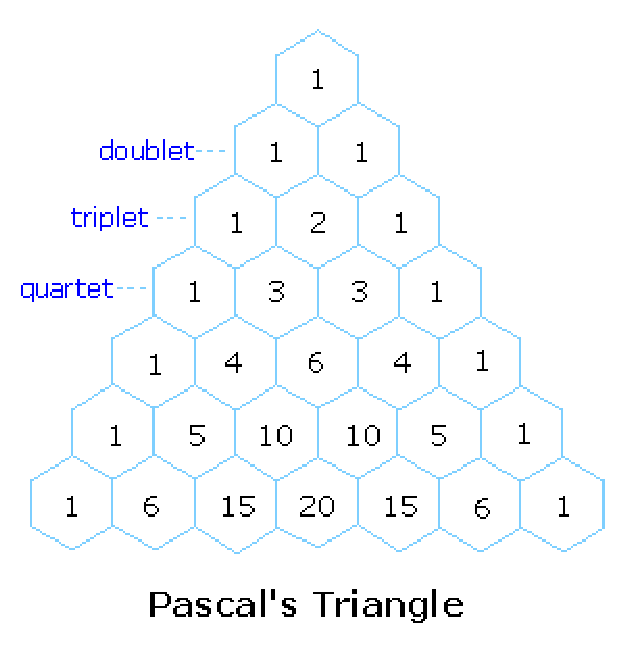
\includegraphics[width=0.7\textwidth]{espectro_pascal}
   \caption{El triángulo de Pascal es un gráfico que se utiliza, en RMN, para predecir el ratio de altura entre los picos de spines separados en el espectro. Puede observarse que cada hexágono representa la suma de los dos hexágonos contiguos superiores.}
 \label{fig:espectro_pascal}
 \end{figg}
\end{figure}

 




\begin{figure}[htb]
 \begin{figg}
   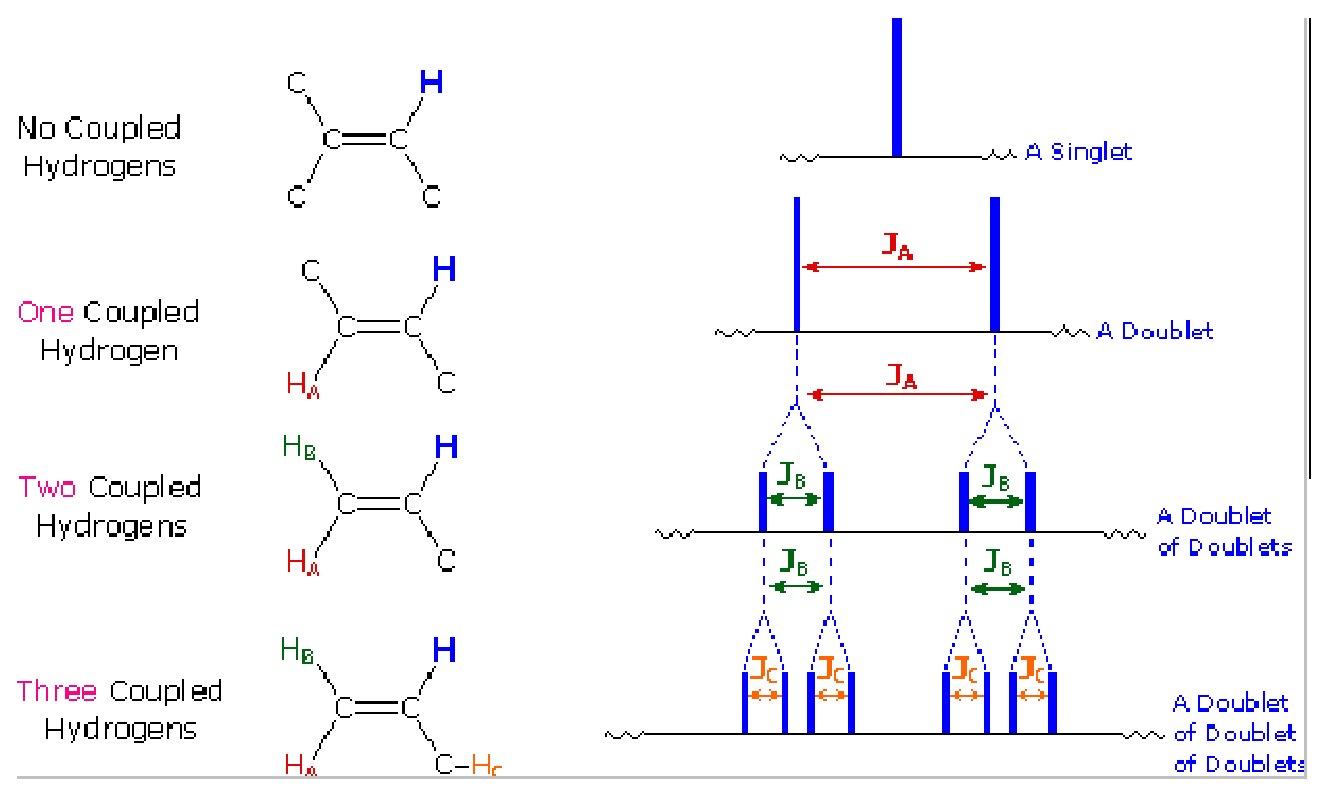
\includegraphics[width=0.7\textwidth]{espectro_couplingComplex}
   \caption{Las diferentes interacciones entre los núcleos lleva a configuraciones más complejas, como se muestra en la imagen. Cada H de un color representa una constante J distintinta (del mismo color al H).}
 \label{fig:espectro_couplingComplex}
 \end{figg}
\end{figure}





A pesar de que esta técnica solo detecte protones de H, podemos aprovechar las características del espectro anteriormente mencionadas para poder determinar los componentes presentes en la muestra, ya que podemos detectar la cantidad de protones de H y diferenciar los que no son isocrónicos y saber del emparejamiento de estos. Además podemos comparar el espectro resultante con otros espectros ya realizados, pudiendo consultar una base de datos de espectros preexistente.


\section{Espectroscopía por RMN in vivo}
Al igual que las técnicas de iRMN para la espectroscopía por RMN requiere de:

\begin{itemize}
  \item Un intenso campo magnético homogéneo
  \item Un transmisor de Radio Frecuencia capaz de producir pulsos cortos
  \item Un receptor sensible para amplificar al señal de RMN
  \item Un digitalizador de la señal 
  \item Un programador de pulsos
  \item Una computadora para el control y análisis de los datos
  \item Un ``contenedor'' que permita la excitación de la muestra a través de las bobinas
\end{itemize}


Sin embargo el contenedor de la muestra no tiene por qué ser un contenedor físico. Gracias a las técnicas de codificación espacial de iRMN podemos establecer un contenedor virtual que delimite un área de interés y solo recibiremos señal de dicha muestra contenida. Gracias a este proceso podemos realizar espectroscopía por RMN in vivo, ya que no necesitamos extraer físicamente la muestra del paciente (como en una biopsia). El contenedor virtual no es más que un voxel, el cual podemos determinar su tamaño y localización gracias a gradientes en la magnetización. A diferencia de iRMN, donde se excita selectivamente una rebanada y con gradientes de magnetización se obtiene una señal que luego se codifica espacialmente (dentro de esa rebanada), en la espectroscopía por RMN  se excita selectivamente tres planos ortogonales y es donde estos tres se superponen que queda determinado el voxel o volumen de interés (y por tanto será el único lugar de donde tendremos señal). Este método se llama SVS (single Voxel Spectroscopy)

\begin{figure}[htb]
 \begin{figg}
   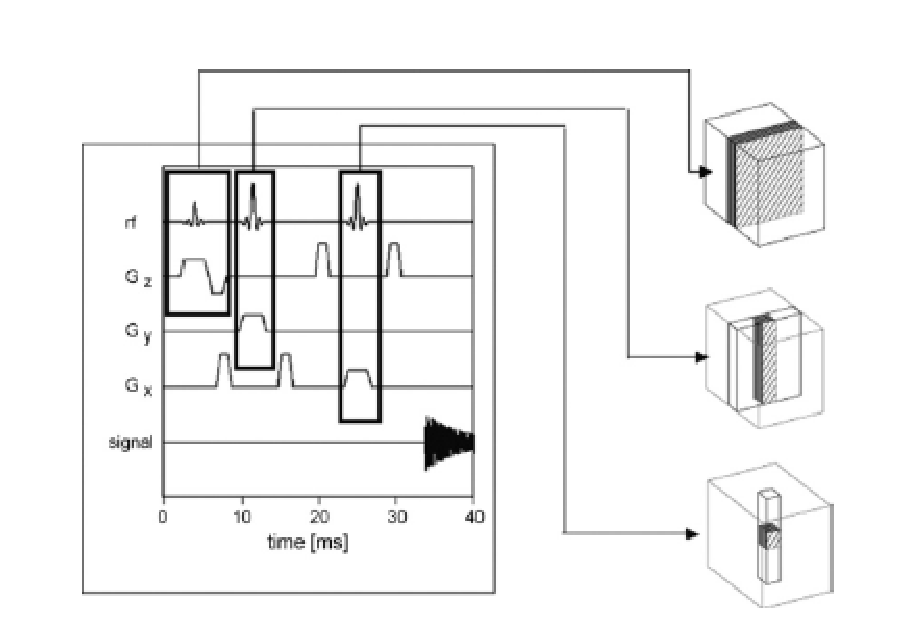
\includegraphics[width=0.7\textwidth]{espectro_singleVoxel}
   \caption{Esquema representativo de la secuencia para la obtención de un voxel o volumen de interés. Observese que el voxel resultante es producto de la superposición de los 3 planos ortogonales. Este voxel será el único volumen que reciba todos los requisitos para emitir señal.}
 \label{fig:espectro_singleVoxel}
 \end{figg}
\end{figure}





En espectroscopía por RMN se utilizan principalmente dos secuencias PRESS (pointed-resolved spectroscopy) y STEAM (stimulated echo acquisition mode).


\subsection{PRESS}
La secuencia más utilizada es PRESS. En esta, el espectro se obtiene con un pulso de 90º seguido de otros dos de 180\degrees. Cada uno de ellos es aplicado al mismo tiempo con diferentes gradientes magnéticos. Entonces, la señal emitida por el voxel es un spin eco. El primer pulso de 180\degrees se aplica después de un tiempo $1/2TE$ después del primer pulso de 90\degrees, i el segundo pulso de 180\degrees se aplica después de un tiempo $1/2TE + TE$. La señal se produce después del tiempo $2TE$. Para restringir la adquisición a un solo voxel, se requieren gradientes destructores. Los gradientes destructores desfasan los núcleos fuera del voxel de interés y reducen la señal.



\begin{figure}[htb]
 \begin{figg}
   \includegraphics[width=0.7\textwidth]{espectro_press}
   \caption{Secuencia PRESS.}
 \label{fig:espectro_press}
 \end{figg}
\end{figure}






\subsection{STEAM}
Dado que la secuencia STEAM solo usa pulsos de 90\degrees, tiene un 50\% menos de ratio señal-ruido (SNR, de signal-noise ratio) que PRESS.  Los pulsos de 180\degrees  resultan en un voxel menos óptimo y conllevan un SNR más alto. Sin embargo, dado que la longitud de los pulsos de 180º son más largos, PRESS no se puede hacer con TE muy cortos. Otro inconveniente de PRESS es que tiene un mayor artefacto de desplazamiento por corrimiento químico.

\begin{figure}[htb]
 \begin{figg}
   \includegraphics[width=0.7\textwidth]{espectro_steam}
   \caption{Secuencia STEAM.}
 \label{fig:espectro_steam}
 \end{figg}
\end{figure}


Si nos interesa un estudio de la distribución espacial (y no de un solo voxel) es posible realizar una espectroscopía multivoxel (MVS) e incluso de puede obtener unas imágenes de espectroscopía de resonancia magnética (MRSI). A diferencia de las imágenes iRMN, el resultado final es una matriz (2D o 3D) con los espectros de cada uno de los voxeles. Para ello solo se requiere un gradiente codificador de fase después del pulso RF en cada una de las dimensiones que se quiera codificar.

Las técnicas SVS resultan en espectros de alta calidad, en un tiempo de escáner corto, y buena homogeneidad de campo. Es decir SVS se utiliza para obtener mediciones precisas de metabolitos. Por otro lado las técnicas MRSI presentan la ventaja de además tener información relativa a la distribución espacial, pero la cuantificación de metabolitos no es tan precisa debido al sangrado de voxeles (el espectro dado por un voxel puede presentar contribución de otras regiones espaciales). Por eso MRSI se suele utilizar para determinar heterogeneidad espacial.

% SVS
% MRSI
% TE corto
% TE largo
% 1 voxel
% Multi-voxel
% Región limitada
% Adquisición múltiple de datos
% Área fija
% Cuadrícula movible tras adquisición
% Más precisa
% Sangrado del voxel
% Mediciones cuantitativas
% Distribución espacial


\subsection{TE para MRS}
Las MRS se pueden obtener con diferentes TE, dando diferentes espectros.
Con TE cortos (20-40ms) tienen mayor SNR y menos pérdida de señal debido al peso de T2 y T1 (en comparación con TE largos). Así pues los espectros con TE cortos presentan más picos de metabolitos, que no se detectan con espectros de TE largos. Sin embargo dado el mayor número de picos, estos puede presentar solapamiento (importante tener en cuenta a la hora de cuantificar).
Con TE largos (135-288 ms) hay peor SNR, sin embargo tienen espectros más simples debido a la supresión de señal. 


\begin{figure}[htb]
 \begin{figg}
   \includegraphics[width=0.7\textwidth]{espectro_TEs}
   \caption{Comparación entre dos espectros de la misma muestra con diferentes TE. A) Espectro con TE=30 ms. B) Espectro tomado con TE=135 ms.}
 \label{fig:espectro_TEs}
 \end{figg}
\end{figure}






En cerebro el agua es muy abundante, siendo su señal en el espectro de MRS mucho más alta que los otros metabolitos. Para evitar la superposición del pico del agua con otros picos de otros metabolitos se requiere de técnicas de supresión de la señal de agua.

\begin{figure}[htb]
 \begin{figg}
   \includegraphics[width=0.7\textwidth]{espectro_aguaLipido}
   \caption{Como se observa en el gráfico, la señal obtenida de agua y lípidos son mucho mayores que las moléculas de interés en espectroscopía. Es por eso que se requiere de mecanismos para evitar que su señal enmascare o influya de algún modo en el espectro.}
 \label{fig:espectro_aguaLipido}
 \end{figg}
\end{figure}




La secuencia más común para ello es CHESS (chemical shift selective water suppression), en la cual se pre-satura la señal del agua usando frecuencias selectivas de pulsos de 90º antes de la secuencia de pulsos de localización. Otra secuencia es VAPOR (VAriable Pulse power and Optimized Relaxation Delays) y WET (Water suppression Enhanced Through T1 effects)

\begin{figure}[htb]
 \begin{figg}
   \includegraphics[width=0.7\textwidth]{espectro_CHESS}
   \caption{Comparación entre espectros con y sin suprimir la señal del agua. Antes de la secuencia CHESS (A) y después de la secuencia CHESS (B).}
 \label{fig:espectro_CHESS}
 \end{figg}
\end{figure}




\section{Artefactos en espectroscopía por RMN}
La espectroscopía por RMN también está sujeta a la aparición de artefactos. Des de la mala supresión de la señal de agua o lípidos, inhomogeneidad del campo magnético, corrientes de Eddy a desplazamiento por corrimiento químico, son algunos de los factores que introducen artefactos en espectro.
Lo más importante es la homogeneidad del campo magnético, pues una baja homogeneidad reduce el SNR y aumenta la anchura de los picos. Algunos lugares son más susceptibles a este fenómeno, cerca del hueso o de interficie tejido-aire. Se recomienda evitar estos lugares al determinar nuestro Volumen de interés.
Los corrientes de Eddy que se causan por el encendido de los gradientes, provocan también artefactos. Un corriente de transito resulta en la distorsión de la forma de los picos, haciendo difícil la cuantificación del espectro.
El desplazamiento por corrimiento químico puede provocar artefactos. La localización del voxel está basada en la frecuencia de precesión de los protones. Dado que estas frecuencias son diferentes para cada metabolito, la posición exacta de dichos metabolitos será ligeramente diferente. Para resolver este problema, se requiere de gradientes de campo fuertes para la selección de rebanada.




\section{Metabolitos en el cerebro}
La espectroscopía por RMN permite la detección de metabolitos en el cerebro. Cambios en estos metabolitos delatan anormalidades estructurales. Para saber de estos cambios se requiere conocer los espectros del cerebro en estado normal y sus diferentes variantes dependiendo de técnicas, edad del sujeto, regiones cerebrales, etc.
A continuación trataremos algunos metabolitos de interés analítico en el cerebro, y la Tabla \ref{tab_espectro_metabolitos} muestra un resumen de los hallazgos más comunes en espectroscopía en presencia de anormalidades tisulares específicas.

\subsection{N-acetilaspartato (NAA)}
El pico de NAA es el más alto del espectro del cerebro normal. Este pico está alrededor de  2,02 ppm. Se sintetiza en la mitocondria de las neuronas y es transportado al citoplasma a lo largo del axón. Es un metabolito exclusivo del sistema nervioso central (SNC), tanto en sustancia blanca como gris. Es un marcador de densidad y viabilidad neuronal y axonal. Puede encontrarse en oligodendrocitos inmaduros y células progenitoras de astrocitos.
La ausencia o reducción de la concentración de NAA es señal de pérdida o degradación neuronal. Por otro lado, su incremento es específico de la enfermedad de Canavan.

\subsection{Creatina (Cr)}
El pico de Cr se asigna a 3,02 ppm. Este pico representa una combinación de moléculas que contienen  creatina y fosfocreatina. Es un marcador metabólico intracelular y del sistema energético. La concentración de Cr es relativamente constante y muy estable. Se utiliza como referencia interna para calcular ratios con otros metabolitos.
En tumores cerebrales, hay reducción de la señal de Cr. Por otro lado la gliosis puede producir un incremento mínimo, dado el incremento de la densidad de células gliales (proliferación de la glia). Enfermedades sistémicas pueden afectar también la concentración de CR en el cerebro.

\subsection{Colina (Cho)}
Se asigna al pico de 3,22 ppm y representa la suma de Cho y compuestos que contengan Cho. Es un marcador de recambio de la membrana celular, reflejando proliferación celular. En tumores, los niveles de Cho correlacionan con el grado de malignidad. El aumento de Cho pude aparecer también en infarto o inflamación.
Lactato (Lac)
El pico del Lac no parece en un espectro del cerebro “normal”, o es casi inapreciable. EL pico del Lac es un doblete en 1,33 ppm, el cual proyecta por encima de la línea base cuando se adquiere con TE cortos/largos, pero se invierte con TE de 135-144 ms. Lac se produce por glicolisis anaeróbica, por tanto su presencia en cerebro indica hipoxia, isquemia, epilepsia y desordenes metabólicos. También hay aumento por acumulación de macrófagos (inflamación). Este también se acumula en tejidos con bajo recambio de fluido, como cistos.

\subsection{Lipidos (Lip)}
Los Lipidos son componentes de membrana, estos no pueden ser visualizados con TE largos, debido a su corto tiempo de relajación. Hay dos picos de lípidos: a 1,3 ppm se encuentra los que contienen grupos metilenos, y a 0,9ppm los que contienen grupos metil. Estos picos están ausentes en el cerebro normal. Los picos de lípidos pueden observarse cuando se rompe la membrana celular o por necrosis, como ocurre en metástasis y tumores malignos.

\subsection{Mioinositol (Myo)}
Myo es un azúcar simple asignado al pico 3,56 ppm. Se considera un marcador glial dado que es principalmente sintetizado en células gliales (prácticamente solo astrocitos). Es también el osmolito más importante en astrocitos. Myo puede representar el producto de la degradación de la mielina. Altos niveles de Myo se presentan cuando ocurre una proliferación de células gliales o aumento del tamaño de estas (inflamación). Los niveles de Myo se presentan elevado en gliosis, astrocitosis y la enfermedad de Alzheimer.

\subsection{Alanina (Ala)}
Ala es un aminoácido que presenta un doblete centrado en 1,48 ppm. Este pico se encuentre por encima de la línea base en espectros adquiridos con TE corto/largo, y se invierte por debajo cuando se adquiere con TE de 135-144 ms. Su pico puede verse enmascarado por Lac (a 1,33 ppm). LA función de Ala es incierta pero juega un rol en el ciclo del ácido cítrico. Un aumento en la concentración de Ala puede ocurrir por algún defecto en el metabolismo oxidativo. En tumores este aumento es específico de meningiomas.
Glutmato-Glutamina (Glx)
Glx es un pico complejo de Glutamato (Glu), Glutamina (Gln) y ácido gamma-aminobutírico asignado al pico de 2,05 a 2,50 ppm. Estos metabolitos son muy difíciles de separar a 1,5T. Glu es un neurotransmisor excitatorio muy importante y también juega un papel en el ciclo redox. Concentraciones elevadas de Gln se encuentran en algunas pocas enfermedades como en encefalopatía hepática.
El principal uso de la espectroscopía por RMN del cerebro es el de diagnóstico. Gracias a la espectroscopía por RMN se pueden observar cambios en los metabolitos previamente nombrados, con la enorme ventaja de no necesitar abrir el cráneo.



\begin{table}[htbp]
\centering
\caption{Tabla que muestra diagnosis de tumores en base a cambios en el espectrode RMN. \textuparrow  Pico aumentado; \textdownarrow  Pico disminuido; N Pico normal. 1: NAA ausente en el centro del tumor. 2: La presencia de Lac depende del grado del tumor. 
3: Lac y Glu se encuentran aumentados solo en estados iniciales de la enfermedad.}
\label{tab_espectro_metabolitos}
\begin{tabular}{@{}lcccccccccc@{}}
\toprule
                     & Cho & NAA & Lac & Lip & Myo & Glu & Suc & Acet & Ala & Aa \\ \midrule
Tumor de bajo grado  & \textuparrow   & \textdownarrow   &     &     & \textuparrow   &     &     &      &     &    \\
Tumor de alto grado  & \textuparrow   & \textdownarrow   & \textuparrow   & \textuparrow   &     &     &     &      &     &    \\
Metastasis           & \textuparrow   & \textuparrow$^1$  & \textuparrow   & \textuparrow   &     &     &     &      &     &    \\
Oligodendroglioma    & \textuparrow   & \textdownarrow   & \textuparrow$^2$  &     &     &     &     &      &     &    \\
Meningioma           & \textuparrow   & \textuparrow   &     &     &     &     &     &      & \textuparrow   &    \\
Gliomatosis cerebral & \textuparrow   & \textdownarrow   &     &     &     &     &     &      &     &    \\
Linfoma              & \textuparrow   & \textuparrow$^1$  &     & \textuparrow   &     &     &     &      &     &    \\
Radionecrosis        & \textdownarrow   & \textdownarrow   & \textuparrow   & \textuparrow   &     &     &     &      &     &    \\
Abcesos              & N   & \textdownarrow   & \textuparrow   & \textuparrow   &     &     & \textuparrow   & \textuparrow    & \textuparrow   & \textuparrow  \\
Desmelinización      & \textuparrow   & \textdownarrow   & \textuparrow$^3$  & \textuparrow   & \textuparrow   & \textuparrow$^3$  &     &      &     &    \\ \bottomrule
\end{tabular}
\end{table}




% Lecturas recomendadas
% The basics of MRI, Joseph P. Hornak (1996-2014).
% 1H MR Spectroscopy of the Brain: Absolute Quantification of Metabolites, Jacobus F. A. et al., Radiology (2006).
% Brain Proton Magnetic Resonance Spectroscopy, Débora Bertholdo, University of North Carolina at Chapel Hill. *(http://www.ajnr.org/site/fellows/files/MRS-chapter-Castillo.pdf)
% MRI From Picture to Proton, Donald W. McRobbie et al., Cambridge University Press 2ª Ed. (2006).
% 
% Páginas web recomendadas
%  http://orgchem.colorado.edu/Spectroscopy/
% http://www-keeler.ch.cam.ac.uk/lectures/Irvine/
% https://www2.chemistry.msu.edu/faculty/reusch/virttxtjml/Spectrpy/spectro.htm

\chapter{Artefactos de imagen}
\chapterprecis{\noindent Luis Concha\\Instituto de Neurobiología\\UNAM, Campus Juriquilla}
\label{chapter_artefactos}





\part{Protocolos de Imagen, aplicaciones y diseño experimental}
\label{part_protocolos}


\chapter{Resonancia magnética funcional: Origen de la señal BOLD}
\label{chapter_bold}
\chapterprecis{\noindent Juan Carlos Méndez, Ramón Bartolo\\Instituto de Neurobiología\\UNAM, Campus Juriquilla}

Varias técnicas de neuroimagen permiten medir cambios fisiológicos asociados al aumento de la actividad de grupos neuronales. Sin embargo, cuando se piensa en estudios funcionales del cerebro mediante resonancia magnética (fMRI), normalmente se piensa en estudios que utilizan la señal BOLD (señal dependiente del nivel de oxígeno en sangre por sus siglas en inglés: Blood Oxygen Level Dependent). Descubierto en 1990 por Ogawa y cols. \cite{OgawaS1990}, el fenómeno rápidamente se ha convertido en el estándar de medición de la actividad de grupos neuronales durante la ejecución de una gran variedad de tareas sensoriomotoras y cognitivas. Una búsqueda realizada en \emph{Pubmed} en noviembre de 2011 con el término fMRI arroja cerca de 300 mil resultados. Existen varias razones para el éxito de esta técnica, entre ellas, el hecho de no ser invasiva y su buena resolución espacio-temporal en comparación con otros métodos usados en humanos. Sin embargo, aún no existe un acuerdo entre la comunidad neurocientífica en cuanto al origen de esta señal y su relación con la actividad neuronal. En este capítulo discutiremos brevemente cómo se origina la señal BOLD en el resonador. Después discutiremos cómo se acopla el flujo hemodinámico con los cambios en la actividad neuronal, y finalmente trataremos los avances que nos han acercado a la comprensión de qué procesos neuronales específicos son los que generan los cambios hemodinámicos observados en la fMRI.

\section{La señal BOLD}
Durante un estudio de resonancia magnética, los diferentes componentes de los tejidos se magnetizan en mayor o menor medida, causando inhomogeneidades en el campo magnético local. El grado de magnetización de cada material depende de su susceptibilidad magnética; aquellos materiales con susceptibilidades magnéticas fuertes, llamados materiales ferromagnéticos, se magnetizan más fácilmente que aquellos con susceptibilidades magnéticas débiles, llamados paramagnéticos. Los materiales diamagnéticos tienen una susceptibilidad prácticamente nula \cite{Runge2009}. La relajación transversal de las partículas de un tejido sometido al campo magnético \Bzero y a un pulso de radiofrecuencia está dada en gran medida por estas inhomogeneidades magnéticas . A la constante que mide este decaimiento transversal se le conoce como \Ttwostar. Mientras mayor sea la susceptibilidad magnética, más rápido será el decaimiento y menor señal brindará esa zona del tejido. En el cerebro constantemente se modifican las inhomogeneidades dependiendo de su estado fisiológico, particularmente en función de la relación oxihemoglobina/desoxihemoglobina de la sangre local \cite{LogothetisNK2004}. Esto se debe a que la hemoglobina oxigenada es diamagnética, pero a medida que se consume el oxígeno que transporta, queda expuesto el hierro que forma parte central de la hemoglobina, cambiando su susceptibilidad magnética. Por lo tanto, la desoxihemoglobina (dHb) es paramagnética e influye en la señal de resonancia incrementando el \Ttwostar. Finalmente, la composición de la sangre en una región particular del cerebro depende de la actividad neuronal local. Por esta razón, el \Ttwostar es una medida indirecta de la actividad neuronal y es la base del contraste BOLD. 

El contraste BOLD surge de la mayor cantidad de oxihemoglobina que hay en los capilares y las vénulas que drenan zonas de actividad neuronal aumentada. Esto podría parecer contraintuitivo. En aquellas zonas con mayor actividad cabría esperar un aumento en la concentración de dHB debido al aumento en el metabolismo de esa región. Sin embargo, ocurre también un aumento en el flujo sanguíneo cerebral que sobrecompensa la disminución en la concentración de oxígeno \cite{LogothetisNK2004}. Es importante mencionar que en neonatos esta relación está invertida y la concentración local de dHb incrementa con la actividad neuronal \cite{PM2001}. El contraste BOLD inicia aproximadamente 2 s después de la activación, llega a una meseta 7 s después y regresa posteriormente a la línea basal, algunas veces con la aparición de una disminución post-estímulo \cite{LogothetisNK2004}.


\section{La respuesta hemodinámica y su acople con la actividad metabólica cerebral}
En condiciones normales, el cerebro obtiene prácticamente toda su energía de la oxidación de glucosa. Esto requiere un suministro constante de glucosa y oxígeno, que se realiza a través de la sangre que fluye por una red densa de vasos sanguíneos. El cerebro constituye alrededor del 2\% de la masa corporal, sin embargo, su consumo de glucosa y oxígeno es más o menos el 20\% del consumo total en el cuerpo \cite{A2001}. Conviene hacer énfasis en el hecho de que existe un acople preciso, mas no lineal, entre la actividad neuronal y el flujo sanguíneo local.

Entender cómo la respuesta hemodinámica se acopla a la actividad neuronal es necesario para la correcta interpretación de imágenes funcionales que utilizan la señal BOLD, y esto implica el entendimiento de los mecanismos que regulan el flujo sanguíneo local en el cerebro. En principio, múltiples mecanismos interactúan en el control de dicho proceso. Por un lado, en la perfusión global del cerebro participan mecanismos autonómicos (\emph{v. gr.} simpáticos)  y hormonales (por ejemplo, el sistema renina-angiotensina). La perfusión local requiere de mecanismos de regulación más específicos para lidiar con los cambios en la demanda energética del tejido ocasionados por cambios transitorios en la actividad neuronal. Entre los factores que pueden estar involucrados en la generación de una respuesta local está el potasio liberado al espacio extracelular durante la despolarización neuronal. El óxido nítrico, principalmente  el producido en las neuronas, es probablemente la señal química más importante que permite una comunicación directa entre las neuronas y los vasos sanguíneos para generar cambios locales en la perfusión sanguínea.

Si no consideramos al óxido nítrico, la comunicación entre las neuronas y los vasos sanguíneos requiere de un mediador, ya que no existe contacto directo entre ellos. Los astrocitos poseen numerosos procesos que envuelven una gran cantidad de procesos neuronales y sinapsis. En la corteza cerebral humana, se calcula que un solo astrocito podría monitorear y regular el funcionamiento de más de 1 millón de sinapsis \cite{OberheimNA2006}. Más aún, cada astrocito posee al menos un proceso que envuelve un vaso sanguíneo \cite{SimardM2003}, al que se llama ``pie vascular''. Esta relación anatómica sugiere que los astrocitos juegan un papel crucial en la regulación del flujo sanguíneo cerebral. Valga también mencionar que los astrocitos pueden formar un continuo comunicándose entre ellos mediante uniones comunicantes (\emph{gap junctions}), y de este modo integrar la actividad neuronal a gran escala. Por lo tanto, su papel resulta crucial para la modulación del flujo sanguíneo, de tal modo que se mantenga un aporte constante de nutrientes y oxígeno que permita el adecuado funcionamiento de poblaciones neuronales grandes.

Al parecer, los factores mencionados interactúan de manera compleja para generar una respuesta hemodinámica que permita satisfacer las demandas metabólicas neuronales derivadas de un incremento en su actividad. Abordamos en este escrito los factores más estudiados, sin que esto implique que sean los únicos involucrados en la regulación de la respuesta hemodinámica.

\subsection{Señalización por óxido nítrico (NO)}
El óxido nítrico es un potente vasodilatador que se produce en cantidad proporcional a la cantidad de calcio libre, tanto en neuronas como en células endoteliales. La síntesis del  NO es catalizada por  óxido-nítrico-sintetasas (NOS) específicas de cada tipo celular, nNOS en neuronas y eNOS en células del endotelio vascular.  Numerosos estudios de estimulación somatosensorial en animales anestesiados (ver Toda \emph{et al}.\cite{TodaN2009}) han mostrado que la activación neuronal ocasiona una respuesta hemodinámica asociada al incremento de NO en la región estudiada de la corteza somatosensorial primaria. Se ha observado que la respuesta hemodinámica se reduce dramáticamente utilizando inhibidores de la nNOS. Al parecer, la eNOS está poco involucrada en el acople entre la actividad neuronal y el flujo sanguíneo local, aunque participa de manera importante en la regulación del tono vascular.

Se cree que el NO derivado de la nNOS afecta de manera directa al músculo liso vascular. Sin embargo, el NO es una molécula altamente reactiva, por lo que su papel en la modulación de la respuesta hemodinámica sería espacialmente muy limitado. No obstante, es posible que el NO también pueda actuar a través de los astrocitos, aunque esto no ha sido estudiado \cite{KoehlerRC2009}.

\subsection{Señalización por potasio}
Es bien sabido que el mantenimiento de una concentración constante de potasio en el medio extracelular es una de las funciones de los astrocitos. Elevaciones de la concentración extracelular de potasio derivadas de la generación de potenciales de acción son contrarrestadas por la activación de canales de potasio rectificadores de entrada (KIR) que se encuentran en el astrocito.

Se ha planteado la hipótesis de que derivado de esta función el astrocito actuaría como un sifón de potasio \cite{PaulsonOB1987}. Al incrementarse la concentración intraastrocítica de potasio en los procesos que rodean a las neuronas, el potasio difundiría hacia los procesos que forman los pies vasculares que rodean a los vasos sanguíneos. Al haber una alta concentración de potasio en el pie vascular, es liberado al espacio extracelular, ocasionando una hiperpolarización de las células del músculo liso vascular, lo que lleva a una vasodilatación. No obstante, la hipótesis del sifón de potasio ha sido puesta en duda \cite{MeteaMR2007}, mas la vasodilatación mediada por potasio podría ocurrir por otras vías, como se discutirá más adelante (ver adelante).

\subsection{Incremento de la actividad astrocítica por la captura de glutamato}
Otra de las funciones importantes de los astrocitos es la de retirar el neurotransmisor excitatorio glutamato del espacio sináptico. Esto se lleva a cabo por un transportador que co-transporta sodio y glutamato hacia el interior del astrocito, con el costo de la elevación intracelular de sodio. Esto requiere que el sodio sea bombeado activamente fuera del astrocito por el intercambiador ATPasa-Na/K. Además de la actividad inducida por la necesidad de mantener las concentraciones de sodio y potasio, el astrocito se encarga de degradar el glutamato convirtiéndolo en glutamina. Esta reacción es catalizada por la glutamina sintetasa, a costa de ATP. Así, la captura de glutamato por el astrocito estimula la hidrólisis de ATP tanto por la actividad incrementada de la bomba de sodio/potasio, como por la degradación de glutamato a glutamina \cite{MagistrettiPJ1998,PellerinL1994}.

La hidrólisis del ATP permite que se incrementen los niveles de adenosina. Esto, lleva al incremento de los niveles intracelulares de calcio activando múltiples cascadas de señalización. Una de dichas cascadas llevaría a la liberación de prostaglandinas en el pie vascular del astrocito, que a su vez, promueven la formación de cAMP en las células del músculo liso vascular, lo que tiene un efecto vasodilatador \cite{KoehlerRC2009}.

\subsection{Señalización por glutamato}
Otro mecanismo, más específico, por el cual el glutamato promueve la vasodilatación es la activación de los receptores metabotrópicos de glutamato (mGlu) localizados en la membrana astrocítica. Esto ocasiona que se libere calcio en el interior del astrocito generando ondas de calcio, con la consecuente liberación de prostaglandinas en el pie vascular que se mencionó más arriba. Zonta \emph{et al}.\cite{ZontaM2003} reportaron incrementos de calcio en astrocitos que rodeaban vasos sanguíneos en respuesta a la estimulación neuronal, y que estos incrementos de calcio se asociaban a un incremento del diámetro de los vasos sanguíneos.

Por otro lado, las ondas de calcio activan canales de potasio dependientes de calcio (KCa) en el pie vascular del astrocito. Se han observado incrementos de calcio intracelular en respuesta a estimulación neuronal, o la aplicación de agonistas de receptores mGlu \cite{FilosaJA2004}. Indagando más, se han registrado corrientes de potasio en los pies vasculares de astrocitos, y una fracción alta de la corriente se atribuyó a canales KCa \cite{FilosaJA2006}. Además, se ha observado que bloqueadores de canales KCa disminuyen la respuesta hemodinámica cuando se estimulan las vibrisas de ratas anestesiadas \cite{GerritsRJ2002}. A lo anterior hay que sumar la observación de que bloqueadores de canales de potasio KIR también inhiben la respuesta hemodinámica \cite{FilosaJA2004}.

Así, llegamos a la hipótesis de que al activar receptores mGlu se generan ondas de calcio en el astrocito, que al activar canales KCa  promueven la liberación de potasio al espacio extracelular en cantidad suficiente para que se activen canales KIR  en las células de músculo liso vascular, ocasionando que se hiperpolaricen con el consecuente efecto de vasodilatación.

\section{Procesos neuronales y la señal BOLD}
Uno de los problemas centrales en la investigación sobre el origen del contraste BOLD es el de la determinación de cuáles son específicamente los procesos neuronales que requieren un aumento del flujo sanguíneo cerebral. Cuando se menciona que cierta región cerebral aumenta su actividad durante la ejecución de una tarea particular, pocas veces se especifica si este aumento se refiere a la tasa de disparo de dicha región, a la actividad sináptica o a algún otro evento. Varios procesos involucrados en la codificación de información consumen energía, entre ellos, la generación y propagación de los potenciales de acción, el mantenimiento del potencial de reposo de membrana, la liberación y recaptura de neurotransmisores, el reciclaje de vesículas sinápticas y las corrientes presinápticas de Ca$^{2+}$ \cite{SmithAJ2002}. Este problema se ha abordado desde diferentes perspectivas. Entre los trabajos más importantes al respecto están aquellos que han utilizado diferentes técnicas de medición de actividad neuronal junto con técnicas que cuantifican el flujo cerebral en las mismas condiciones. Diversos experimentos, particularmente aquellos que combinan electrofisiología con neuroimagen, sugieren que la señal BOLD se origina principalmente como consecuencia de un aumento en la actividad sináptica local \cite{NK2003,NK2008,LogothetisNK2004}. Una breve descripción de los tipos de señales electrofisiológicas es necesaria para comprender mejor esta información.

Las técnicas de registro extracelular de la actividad eléctrica cortical han sido empleadas con gran éxito desde mediados del siglo \textsc{XX} para estudiar los correlatos neurofisiológicos de la conducta. Estos registros se realizan mediante microelectrodos cuya punta es capaz de detectar los cambios de voltaje que ocurren en el medio extracelular que circunda a las neuronas. Cuando la punta se encuentra a menos de 140 $\mu$m de distancia de una neurona, la actividad eléctrica de esta neurona predomina sobre el ruido de fondo y pueden detectarse sus potenciales de acción. A esta señal se le conoce como señal unitaria (en inglés\emph{ Single Unit Activity}, SUA) y se obtiene con electrodos cuya punta tiene una impedancia mayor a 1 M$\Omega$. Se pueden obtener también señales asociadas a un número mayor de neuronas y a otro tipo de procesos mediante microelectrodos con una impedancia menor (alrededor de 100 k$\Omega$). La señal multiunitaria (en inglés \emph{Multi-Unit Activity}, MUA) se obtiene al aplicar un filtro pasa-altas con una frecuencia de corte entre 300 y 400 Hz y representa un promedio de los potenciales de acción generados por las neuronas en un radio de entre 140 a 350 $\mu$m alrededor del electrodo. Esto implica que, dependiendo de la zona registrada, la señal es un promedio de la actividad de alrededor de 1,000 neuronas. En cambio, el potencial local de campo (en inglés \emph{Local Field Potential}, LFP) se obtiene al aplicar un filtro pasa-bajas con una frecuencia de corte menor a 200 Hz. Esta señal se ha correlacionado principalmente con los cambios en los voltajes sinápticos locales en un radio de hasta 3 mm alrededor de la punta del electrodo \cite{NK2003,LogothetisNK2004}. Sin embargo, parte de esta señal también ha sido relacionada con los potenciales somato-dendríticos y con los períodos refractarios que ocurren en las neuronas tras la producción de un potencial de acción \cite{NK2003}.

El grupo de Nikos Logothetis ha realizado varios experimentos en los que obtiene simultáneamente los tres tipos de señales neurofisiológicas descritos anteriormente, así como imágenes de fMRI en monos. En general, la amplitud de la señal BOLD incrementa en función tanto de las señales unitarias y multiunitarias como de los potenciales locales de campo. Sin embargo, en todos los experimentos, los potenciales locales de campo tuvieron un poder predictivo mayor del contraste BOLD que las otras dos señales. Este y otros resultados indican que la señal BOLD refleja principalmente la entrada y procesamiento local de información, más que la señal de salida que es transmitida a otras regiones \cite{NK2003,NK2008,LogothetisNK2004}. Sin embargo, otros experimentos también han correlacionado la tasa de disparo de neuronas individuales con la señal BOLD. Smith y cols. \cite{SmithAJ2002} midieron los cambios locales en el metabolismo cerebral oxidativo mediante fMRI ($\Delta CMR_{O2}/CMR_{O2}$) y simultáneamente realizaron registros extracelulares unitarios. Encontraron que los cambios en la tasa de disparo de la población neuronal registrada se veían acompañados por cambios equivalentes en el metabolismo cerebral.

Ahora bien, mientras que el 90\% de las sinapsis corticales son excitatorias, el procesamiento local de información está dado por una gran variedad de neuronas tanto excitatorias como inhibitorias. ¿Cuál de estas neuronas es la responsable de la señal BOLD? Para responder a esta pregunta, Lee y cols. \cite{LeeJH2010} recurrieron a técnicas de optogenética. En neuronas piramidales de la corteza motora de ratas indujeron la expresión membranal de canales conocidos como opsinas, los cuales se abren al ser estimulados con luz con rangos de longitud de onda particulares despolarizando a la célula. Simultáneamente, se obtuvieron imágenes de fMRI con contraste BOLD en un resonador de 7T. La activación selectiva de la población que expresaba las opsinas generó una señal BOLD con una cinética muy similar a la observada en registros de activación de la corteza motora durante la ejecución de movimientos. Cuando repitieron este experimento induciendo la expresión de opsinas en interneuronas GABAérgicas, el resultado fue una señal BOLD incrementada en el centro de la zona estimulada pero disminuida en la periferia. En conjunto, estos resultados indican que las neuronas piramidales tienen un papel preponderante en la generación del contraste BOLD.

\section{Conclusiones}
A pesar del gran éxito y de la indudable utilidad de los estudios de resonancia magnética funcional, aún existen muchas interrogantes en cuanto a la naturaleza de la información que se obtiene a través de ellos y su interpretación. Actualmente sabemos que el contraste BOLD se origina por una sobrecompensación en la cantidad de oxihemoglobina que llega a un área que ha incrementado su actividad neuronal, principalmente la actividad sináptica. El acople entre la función de las neuronas y el flujo sanguíneo cerebral está dado por múltiples vías que involucran a la glía, principalmente a los astrocitos, y a una gran cantidad de moléculas, entre las que destacan el óxido nítrico, el glutamato y el potasio. Obviamente, estas vías van de la mano con los cambios en el metabolismo celular, los cuales a su vez son una función de la actividad neuronal. Sin duda, mientras más se avance en el conocimiento de las limitaciones y capacidades de la fMRI, mejor uso podremos darle a esta poderosa herramienta para el estudio de las funciones del cerebro humano, tanto en condiciones normales como patológicas. 
\label{cap:origenBold}


\chapter{Resonancia magnética funcional: Modelo lineal general}
\chapterprecis{\noindent Zeus Gracia Tabuenca\\Instituto de Neurobiología\\UNAM, Campus Juriquilla}
% \documentclass{article}
% \usepackage[utf8]{inputenc}
% \usepackage[spanish]{babel}
% \usepackage{hyperref} % Allows hyperlinks
% 
% \usepackage[style=authoryear,sorting=nyt]{biblatex}
% \addbibresource{biblio.bib}
% \usepackage{csquotes} % 'babel/polyglossia' detected but 'csquotes' missing. Loading 'csquotes' recommended.
% 
% \title{Modelo lineal general}
% \author{Zeus Chiripa}
% \date{Octubre 2017}

% \begin{document}

% \maketitle

\section{Introducción}

El modelo lineal general (GLM, por sus siglas en inglés) es uno de los análisis estadísticos por excelencia en los datos obtenidos mediante técnicas de imagen cerebral. Los GLM son una herramienta estadística muy flexible y que pueden ser aplicados para evaluar métodos de efectos fijos como por ejemplo regresiones múltiples, análisis de varianza multivariante (MANOVA) o análisis de covarianza (MANCOVA). Además, y a pesar de su apelativo de lineal, este tipo de modelos pueden introducir elementos no lineales \cite{chung2013statistical}.

Los GLM permiten evaluar de una manera sencilla y eficaz relaciones entre variables a la vez que toma en cuenta el posible efecto de una covariable, es decir, una variable que no es de interés directo sobre el efecto a estudiar. Por ende, el GLM es una herramienta estadística muy completa para comprobar hipótesis entre variables. Por ejemplo, el GLM aplicado a los datos obtenidos mediante imágenes de resonancia magnética funcional (fMRI) permite ajustar con relativa sencillez otros modelos estadísticos como la función de la respuesta hemodinámica (HRF, por sus siglas en inglés) en un estudio relacionado a eventos o en un diseño por bloques \cite{lazar2008statistical}.

El GLM se define de la siguiente manera:

\begin{center}
  $Y = X\cdot\beta + \epsilon$
\end{center}

Donde $Y$ es la respuesta a modelar, $X$ es la matriz de variables predictoras, $\beta$ son los coeficientes asociados a cada una de las variables predictoras y $\epsilon$ representa al error, que por lo general se asume que tiene una distribución normal con media cero y varianza conocida ($\sigma^2$).

En fMRI, por lo general, $Y$ suele ser la matriz de datos, i.e., una matriz con el valor obtenido por cada voxel\footnote{\textit{Voxel}: es la unidad de información gráfica que define un punto dentro de un espacio tridimensional. En resonancia magnética corresponde a los puntos dentro del volumen que corresponde a la imagen.} a lo largo del tiempo (i.e., por cada tiempo de muestreo o \textit{time point} [Tp]); $X$ suele representar una matriz con los estímulos presentados a lo largo del tiempo, i.e., la matriz del diseño experimental. Por consiguiente, este modelo asume que los datos obtenidos por fMRI pueden explicarse por una combinación lineal de las variables del diseño experimental con un error estadísticamente normal asociado (que puede interpretarse como ruido gaussiano). En realidad, se trata de una asunción muy reduccionista para un fenómeno tan complejo como son los datos de fMRI, sin embargo, aquí radica una de las principales ventajas del GLM y es su simplicidad, dado que con un cálculo computacionalmente sencillo puede minimizar el error asociado al ajuste del modelo.

De la manera más simplificada, el GLM asume que cada voxel y cada Tp es independiente el uno del otro, y que la varianza del error ($\epsilon$) es constante a lo largo de todos los voxels. En este caso, la estimación de los coeficientes $\beta$ se puede obtener mediante mínimos cuadrados ordinarios.

Sin embargo, $X$ suele ir acompañada de varias covariables además de la distribución del diseño de bloques (e.g., variable binaria: ausencia o no del estímulo). Por lo general, se suele incorporar una predicción de la respuesta hemodinámica, mediante una convolución del diseño experimental con un modelo de HRF. Esta consideración emula el hecho de que la señal dependiente del nivel de oxigenación en sangre (o señal BOLD, por sus siglas en inglés, \cite{OgawaS1990}) no se hace patente inmediatamente tras la presencia del estímulo y que tiene un decaimiento antes de regresar al estado basal (ver más en detalle el Capítulo \ref{cap:origenBold}).

Además de esta implementación, el GLM es bastante flexible a la hora de incluir otras covariables como pueden ser las características específicas de un sujeto, al grupo al que pertenece (e.g., grupo experimental o grupo control), etc. Es decir, no solamente se restringe al análisis individual de un solo sujeto sino que puede generalizarse el mismo modelo para un grupo de sujetos e incluso para evaluar posibles diferencias entre los grupos.


\section{Modelaje de la señal de Resonancia Magnética funcional}

El análisis estadístico de la señal de fMRI es una de las últimas etapas en un estudio de resonancia magnética. Previamente la señal obtenida ha sido corregida y preprocesada (e.g., corrección de movimiento, filtrado, suavizado, normalización a un espacio estándar, etc.), por tanto, hay que tener en cuenta que se trata de una señal de unidades arbitrarias manipulada.

En la figura \ref{fig:glm01} podemos observar como la señal BOLD se ajusta bastante bien con los bloques de una tarea en particular. Sin embargo, como se comentó en el apartado anterior hay un cierto desfase de la señal sobre el bloque debido al comportamiento de la respuesta hemodinámica. Para limitar este efecto se suele aplicar una convolución de un modelo matemático de la HRF a la matriz del diseño ($X$).


\begin{figure}
	\begin{figg}
    \includegraphics [width=0.7\textwidth]{glm_figura01.eps}
    \caption{Señal BOLD (azul) en un único \textit{voxel} a lo largo del tiempo en un estudio de fMRI bajo diseño de bloques (rojo).}
    \label{fig:glm01}
    \end{figg}
\end{figure}


La convolución se trata de una multiplicación aditiva de dos funciones. En este sentido, asumimos que la respuesta hemodinámica cerebral es un sistema que dado un estímulo su respuesta se puede modelar como la multiplicación aditiva lineal de la aparición o no aparición del estímulo (función 1) y un modelo canónico de dicha respuesta, i.e., la HRF (función 2).

En términos generales, podemos definir a un sistema como un proceso donde una señal de entrada es transformada en otra señal de salida. A modo de simplificación podemos asumir que el cerebro es un sistema que procesa las señales de entrada de un modo lineal respecto a las señales de salida. Es decir, podemos modelar el cerebro como un sistema lineal de tiempo invariante o sistema LTI, lo cual va a permitir trabajar de manera muy eficiente con las matrices del GLM \cite{cohen1997parametric}, dado que tiene las propiedades lineales de ser multiplicativo y aditivo, así como de independencia entre las respuestas \cite{vazquez1998nonlinear}.



\begin{figure}
	\begin{figg}
    \includegraphics [width=0.7\textwidth]{glm_figura02.eps}
    \caption{Convolución (cuyo símbolo matemático es un asterisco) de un diseño de bloques con una HRF de doble gamma y su resultado consiguiente.}
    \label{fig:glm02}
    \end{figg}
\end{figure}

En la figura \ref{fig:glm02}, se ilustra un ejemplo de la señal predicha de una señal de entrada (diseño de bloques) que “entra” en un sistema LTI, el cual convoluciona la respuesta hemodinámica, en este caso modelada por una función de doble gamma (\cite{friston1998event}) y su resultado es la señal de salida, el comportamiento esperado de la señal BOLD ante un diseño de bloques.


\begin{figure}
	\begin{figg}
    \includegraphics [width=0.7\textwidth]{glm_figura03.eps}
    \caption{Respuesta hemodinámica (azul) en un único voxel a lo largo del tiempo en un estudio de fMRI y su predicción mediante la convolución de una HRF doble gamma sobre el diseño de bloques (rojo).}
    \label{fig:glm03}
    \end{figg}
\end{figure}


Finalmente, en la figura \ref{fig:glm03} se ilustra la señal esperada al convolucionar la HRF sobre el diseño de los bloques. Se observa que el solapamiento sobre la señal BOLD observada es mejor que si sólo se tiene en cuenta el diseño de los bloques, el cual no asume el desfase inicial y el consecuente decaimiento de la respuesta hemodinámica (figura 1). El GLM toma la convolución del diseño de bloques como una variable predictora en la matriz de diseño ($X$), a modo de hacer una mejor predicción sobre la señal BOLD a lo largo de todos los \textit{voxels} ($Y$).


\section{Aplicación del Modelo Lineal General en un estudio de fMRI}

En este apartado se expone de manera simplificada un experimento de memoria de trabajo (N-back) en un estudio de fMRI para un solo participante\footnote{En el enlace \url{github.com/zchuri} se encuentra un tutorial para aplicar un GLM a datos de fMRI}. El paradigma N-back consiste en la presentación sucesiva de imágenes en este caso el participante tiene que recordar por bloques si la imagen presentada coincide con la anterior (1-back) o bien, con la presentada previa a la anterior (2-back). Por tanto, se va a modelar en base al GLM de modo que:

\begin{itemize}
  \item La variable dependiente ($Y$) será la señal BOLD para cada voxel a lo largo del tiempo.
  \item La matriz de diseño ($X$) constará de dos bloques uno para la tarea 1-back y otro para la tarea 2-back. Donde se convoluciona la presencia o ausencia de dicha tarea a lo largo del tiempo por una HRF de doble gamma.
  \item Los coeficientes para cada parámetro del modelo ($\beta$), es decir, habrá un coeficiente asociado a los bloques 1-back ($\beta_1$) y otro coeficiente asociado a los bloques 2-back ($\beta_2$).
  \item El error asociado al modelo ($\epsilon$), que para asumir que el modelo tiene un buen ajuste debe seguir una distribución normal con media cero.
\end{itemize}

En la figura \ref{fig:glm04} se muestra un esquema del modelo GLM dado los supuestos del experimento en cuestión.

\begin{figure}
	\begin{figg}
    \includegraphics [width=0.7\textwidth]{glm_figura04.eps}
    \caption{Esquema del GLM, abajo, junto con su representación gráfica, arriba, en el experimento de fMRI de memoria de trabajo N-back.}
    \label{fig:glm04}
    \end{figg}
\end{figure}




Una vez que se ha aplicado dicho ajuste a todos los \textit{voxels} de interés el siguiente paso es realizar un análisis estadístico sobre qué tan bueno fue el ajuste. Es decir, se aplica un test estadístico sobre los coeficientes asociados a los parámetros, donde se asume que si el coeficiente es mayor el efecto de su bloque asociado en el ajuste del modelo es mayor. En este ejemplo se va a evaluar una hipótesis para todos los ajustes del modelo: si el coeficiente asociado a la tarea 2-back es mayor a la tarea 1-back. Dado que suponemos que la tarea 2-back es más demandante en términos de memoria de trabajo que la tarea 1-back. Dicha hipótesis sigue una distribución estadística, de modo que si el valor del estadístico resultante del contraste es bajo quiere decir que la diferencia entre ambos coeficientes no es significativamente diferente de cero, mientras que si el valor es suficientemente alto podemos asumir que hay una diferencia significativa entre los bloques y, por consiguiente, concluir que en tales \textit{voxels} su señal BOLD se ajustan al contraste de la hipótesis.

Otro aspecto relevante al considerar la significancia estadística de nuestro modelo sobre los datos observados es el control de los falsos positivos. El modelo va a aplicarse sobre un número ingente de \textit{voxels} (del orden de decenas de miles), por tanto, es necesario llevar a cabo una corrección de múltiples comparaciones. Algunos de los métodos más comunes en los datos de resonancia magnética son el \textit{random field theory}, \textit{false discovery rate} o test de permutaciones \cite{nichols2003controlling,lindquist2008statistical}.

Finalmente, es posible representar espacialmente aquellos \textit{voxels} donde la señal BOLD se ajusta significativamente a los contrastes mediante mapas estadísticos. En los resultados del estudio, se observa la significancia de los coeficientes del contraste en varios cortes axiales. A \textit{grosso modo}, se ve que hay un mejor ajuste del contraste 2-back $>$ 1-back en regiones de la corteza dorsal anterior y posterior, así como en la parte medial del lóbulo frontal (ver detalle en la Figura \ref{fig:glm05}). A las regiones significativas se les aplicó un método de múltiples comparaciones (\textit{family wise error}, o FWE, de \textit{random field theory}). Por tanto, podemos asumir que las regiones señaladas en el mapa estadístico son aquellas donde se recluta una mayor demanda hemodinámica ante tareas de memoria de trabajo tales como el N-back.



\begin{figure}
	\begin{figg}
    \includegraphics [width=0.7\textwidth]{glm_figura05.eps}
    \caption{Mapa de significancia del contraste 2-back $>$ 1-back, donde los valores significativos (p-valor < 0.05; FWE) aparecen en tonos rojo-amarillo. 'R' hace referencia al hemisferio derecho en cada uno de los cortes axiales.}
    \label{fig:glm05}
    \end{figg}
\end{figure}



\section{Conclusión}

De modo breve hemos repasado los parámetros del GLM, el cual sigue unos lineamientos bastante sencillos a pesar de que cuenta con suposiciones bastante rígidas, pero de todos modos, la gran ventaja del GLM es su versatilidad y flexibilidad, además de poseer un cómputo relativamente sencillo (\cite{lindquist2008statistical}).

El capítulo se centró básicamente a la aplicación del GLM en estudios de fMRI y de su consecuente señal BOLD, sin embargo, la aplicación del GLM no acaba aquí, también se puede aplicar a otras técnicas de neuroimagen y además, puede generalizarse al estudio de varios sujetos o varios grupos de interés.

Finalmente, podemos observar un ejemplo sencillo de aplicación del modelo conociendo el diseño de bloques y asumiendo como se va a comportar la respuesta hemodinámica. La gran mayoría de los paquetes que analizan datos de neuroimagen (e incluso cualquier otro tipo de datos) tienen implementados al menos una alternativa de generar el GLM, dado que a pesar de sus desventajas es una herramienta robusta y eficiente para evaluar hipótesis entre variables (\cite{monti2011statistical}).

%--------------------------------
%Bibliography
% \printbibliography

% \end{document}



\chapter{Imágenes sensibles a difusión}
\chapterprecis{\noindent Luis Concha, Penélope Martínez Campo\\Instituto de Neurobiología\\UNAM, Campus Juriquilla}
\label{chapter_difusion}

\footnotetext{Este capítulo se toma en gran parte de la tesis doctoral del autor. University of Alberta, 2007.El texto completo está disponible en \url{personal.inb.unam.mx/lconcha}. El autor agradece a Penélope Martínez Campos por la traducción del texto original.}

\section{Difusión de moléculas de agua}

Todas las moléculas con una temperatura por encima del cero absoluto (es decir, $>$-273.15 \degrees) están en movimiento constante. Este fenómeno fue descrito por primera vez en 1828 por Robert Brown \cite{Brown1828}, basado en la observación del movimiento aleatorio de los granos de polen suspendidos en el agua. Aunque los granos de polen son considerablemente más grandes que las moléculas individuales, el comportamiento descrito por Brown es similar al observado en las moléculas \footnote{De hecho, el movimiento de los granos de polen fue secundario a la difusión del agua moléculas en las que fueron suspendidas.}, por lo tanto, el fenómeno molecular se denomina comúnmente movimiento browniano. La difusión es accionada térmicamente y en el caso más simple es completamente estocástica, con cada molécula describiendo una ``caminata aleatoria'' en el tiempo. Por ejemplo, si una sola molécula de agua suspendida en un mar infinito de agua tranquila pudiera ser seguida a través del tiempo, el camino parecería ser completamente al azar, con probabilidades iguales de ir a cualquier lugar en cada paso del tiempo. Cuanto más tiempo observamos, más lejos podría estar la molécula de agua desde donde comenzó. Sin embargo, con probabilidades iguales de moverse en cualquier dirección, el desplazamiento promedio en el tiempo sería cero.

Albert Einstein resolvió matemáticamente las observaciones de Brown \cite{Einstein1905}. Consideremos varias moléculas de agua que se difunden libremente, cada una con una posición inicial $r$ en el tiempo {$t = 0$}. Si permitimos que  difundan durante un período de tiempo \(\tau\), cada molécula de agua estará entonces en la posición {$r'$}. El coeficiente de difusión {$D$} se puede encontrar por:
Albert Einstein resolvió matemáticamente las observaciones de Brown \cite{Einstein1905}. Consideremos varias moléculas de agua que se difunden libremente, cada una con una posición inicial $r$ en el tiempo {$t = 0$}. Si permitimos que  difundan durante un período de tiempo \(\tau\), cada molécula de agua estará entonces en la posición {$r'$}. El coeficiente de difusión {$D$} se puede encontrar por:

\begin{equation}
D = \frac{1}{6 \tau}  \langle \textbf{R}^T\textbf{R} \rangle
\end{equation}

donde $\textbf{R}$ = {$r'- r$}. El desplazamiento del spin (de los protones en el agua) en el tiempo se considera sobre el conjunto de spins (paréntesis angulados). El desplazamiento en el tiempo {$t$} está dado por la raíz cuadarada del promedio de los desplazamientos al cuadrado ($rms$, por sus siglas en inglés):

\begin{equation}
rms_{n} = \sqrt{2nDt}
\end{equation}
donde {$n$} es el número de dimensiones. El desplazamiento de moléculas de agua en una dimensión se ejemplifica en la Figura \ref{fig:difusion_gaussian} \\

\begin{figure}[htb]
	\begin{figg}
    \includegraphics[width=0.7\textwidth]{gaussianDiffusion.eps}
    \caption{\textbf{Desplazamiento unidimensional de moléculas de agua en el tiempo.} Un número arbitrario de moléculas de agua con posición = 0 en $t = 0$ se difunde con el tiempo. El perfil de desplazamiento gaussiano se amplía a medida que pasa el tiempo.}
    \label{fig:difusion_gaussian}
    \end{figg}
\end{figure}

Recuerde que la difusión es aleatoria (es decir, isotrópica) y, por lo tanto, $D$ es no depende de la dirección a la que se dirige. La magnitud de $D$ depende de la viscosidad y temperatura del medio, y del tamaño de la molécula. El $D$ de agua a 37 \degrees es alrededor de 3.04×10\textsuperscript{-3} mm\textsuperscript{2}/s.\cite{Mills1973}

En el caso de las moléculas de agua, el soluto y el disolvente son la misma molécula, y el fenómeno se denomina autodifusión, para lo cual el modelo de caminata aleatoria simple puede predecir adecuadamente su comportamiento. Ejemplos de auto-difusión de las moléculas de agua se pueden ver en la Figura 2.2. Para el resto de este documento, el término \emph{difusión} se emplea para referirse a la auto-difusión de moléculas de agua.

\begin{figure}
	\begin{figg}
    \includegraphics [width=0.7\textwidth]{isotropicExamples.eps}
    \caption{\textbf{Simulación de caminata aleatoria sobre 100 pasos de tiempo de 3 y 50 moléculas de agua.} La dirección de cada molécula se define aleatoriamente en cada paso. Con el tiempo, las moléculas de agua tienen una probabilidad no nula de visitar cualquier posición en el espacio, pero, en promedio, han movido poco con respecto al origen.}
    \end{figg}
\end{figure}

\subsection{Medición de la difusión con resonancia}

Los efectos de la difusión sobre la señal de RMN se conocen desde la década de 1950, cuando el spin-eco fue descrito por Hahn \cite{Hahn_1950}. Algunos años más tarde, Carr y Purcell publicaron su trabajo sobre medidas cuantitativas T2, en las que reconocen la importancia de la difusión e incluso miden $D$ en una muestra de agua \cite{Carr_1954}. En 1956, Torrey modificó las ecuaciones de Bloch para incluir un término de difusión \cite{Torrey_1956}. Estos primeros intentos de medir $D$ se basaron en el uso de una perturbación constante del campo magnético principal que, entre otros problemas, dificultó la distinción de los efectos relacionados a $D$ de aquellos provocados por la relajación transversal \Ttwo.

Fue el trabajo de Stejskal y Tanner \cite{Stejskal_1965} en los años sesenta lo que facilitó la medición cuantitativa de los coeficientes de difusión molecular mediante el uso de una secuencia de eco de spin con gradientes pulsados (PGSE, Figura \ref{F:stejskal_sequence}). La idea básica es codificar la posición espacial de las moléculas de agua (spins) en $t = 0$, invertir la fase de spin con un pulso $\pi$ y decodificar la posición del spin después del tiempo $\tau$. La posición de los spins (moléculas de agua) es codificada y recodificada con el uso de gradientes de campo magnético (Figura 2.3). Con más detalle: Después de la aplicación de un impulso de radiofrecuencia $\pi/2$ que coloca la magnetización neta en el plano \Mxy con fase cero, se activa un gradiente de campo magnético con amplitud $G$ y duración $\delta$, lo que imparte una fase a los spins según su posición espacial. Como en cualquier eco de spin, un pulso de radiofrecuencia con ángulo $\pi$ (180 \degrees) provoca el refasamiento del ensamble de spins. Un segundo gradiente de campo magnético con las mismas características que el primero (con una separación $\Delta$ con respecto al primero) hace que los spins estáticos (los que no se movieron en el espacio entre ambos pulsos de gradiente) recuperen su fase original. El eco se adquiere en este punto. Si los spins se mueven durante el tiempo entre los dos gradientes del campo magnético (debido a la difusión o a cualquier otra causa), los giros no podrán refasarse completamente, lo que hace que se obtenga menos señal de RMN. Obsérvese que los gradientes de campo se aplican linealmente en una dimensión, proporcionando sensibilización a la difusión sólo a spins que se mueven en esa dirección particular. Es decir, si un spin se mueve perpendicularmente a la dirección del gradiente del campo, no contribuirá a la pérdida de la señal de RMN. La señal puede ser adquirida a través de un eco de spin, como se ha descrito anteriormente, o a través de un eco estimulado \cite{Tanner_1970}. Este último enfoque, que está fuertemente ponderado a \Tone, minimiza la pérdida de señal a través de la relajación transversal, aunque su propia naturaleza se traduce en una reducción del 50\% de la señal original disponible. Se puede también obviar el pulso de radiofrecuencia con ángulo $\pi$, convirtiendo a la secuencia en un eco de gradiente; en este caso el segundo pulso de gradiente debe tener la orientación opuesta al primero ($+G/-G$). Como se revisó en el Capítulo \ref{chapter_relajacion}, los ecos de gradiente proveen menor cantidad de señal, por lo que es mucho más habitual el uso de ecos de spin cuando se codifica la difusión.

Mediante la modificación de las características de la secuencia PGSE, se puede aumentar o disminuir la sensibilidad a la difusión. Si la amplitud de los gradientes se incrementa ($G$), los spins requerirán menos movimiento para experimentar un campo magnético diferente, aumentando así el cambio de fase. Alternativamente, se puede permitir que los spins difundan durante un período de tiempo más largo, aumentando la probabilidad de que los spins se desfasen entre ellos. El tiempo de difusión se expresa como $\Delta - \delta/3$, donde la corrección $\delta/3$ explica la difusión que se produce durante el tiempo en que los gradientes se ejecutan \cite{Stejskal_1965}. La sensibilidad a la difusión se expresa como:
\begin{equation}
b = \gamma^2G^2\delta^2 (\Delta - \frac{\delta}{3})
\label{eq:bval}
\end{equation}
donde $\gamma$ es la relación giromagnética de protones de hidrógeno (42,58 MHz/T). La ecuación \ref{eq:bval} supone que los gradientes de campo local (independiente de los gradientes de difusión-sensibilización) son mínimos en la muestra. En áreas de grandes diferencias de susceptibilidad magnética, se inducen gradientes de campo magnético local. Los gradientes locales impartirían más desplazamientos de fase al spin que no serían totalmente recuperados por el segundo pulso de gradiente, confundiendo la medición de $D$. Cualquier otro gradiente de campo magnético o inhomogeneidad presente durante la secuencia de PGSE debe estar presente y ser idéntico durante la aplicación de ambos gradientes de sensibilización de difusión para poder inferir $D$ correctamente. El límite de tejido entre el aire y el tejido es un ejemplo de este problema (más sobre esto en la Sección \ref{sec:ArtefactosDWI}). Los gradientes sensibilizadores de difusión no tienen que ser rectangulares, como se expresa en la ecuación anterior, en cuyo caso el área del pulso debe ser igual a la del impulso rectangular ideal. El uso de pulsos de gradiente no rectangulares no afecta a la medición de $D$.\cite{Price_1991}

\begin{figure}
	\begin{figg}
    \includegraphics [width=0.7\textwidth] {stejskal_sequence.eps}
    \caption{\textbf{Secuencia de eco de spin con gradientes pulsados (PGSE).} La posición espacial de las moléculas de agua se codifica como fase mediante el uso de un gradiente de campo magnético con duración $\delta$ y magnitud $G$. Un pulso $\pi$ invierte la fase de spin. Un segundo gradiente de campo magnético, idéntico al primero, reenfoca la fase de todos los giros estacionarios. Los giros móviles no experimentan el mismo campo magnético antes y después del pulso $\pi$ de reorientación y el conjunto no se reenfoca homogéneamente, dando como resultado la pérdida de la señal.}
    \label{F:stejskal_sequence}
    \end{figg}
\end{figure}

La cantidad de señal de RMN disponible en un experimento sensible a la difusión decae exponencialmente de acuerdo con $D$ (Figura \ref{F:expDecay_signal_b_2panels}), y se expresa como:

\begin{equation}
\label{eq:bexpdecay}
\frac{S}{S_0} = e^{-bD}
\end{equation}

donde $S$ es la intensidad de señal obtenida con el gradiente de difusión activado y $S_0$ es la intensidad de señal correspondiente obtenida sin el uso de gradientes sensibilizadores de difusión. Esta ecuación también puede expresarse linealmente como:

\begin{equation}
\label{eq:blindecay}
ln (\frac{S}{S_0}) = -bD
\end{equation}\\

\begin{figure}
	\begin{figg}
    \includegraphics [width=0.7\textwidth] {expDecay_signal_b_2panels.eps}
    \caption{\textbf{Señal de RMN de acuerdo al nivel de sensibilización a difusión.} La señal de RMN se representa como una función de $b$ (ecuación \ref{eq:bval}). Se muestran señales de sustancia gris ($D$ = 0.7×10\textsuperscript{-3} mm\textsuperscript{2}/s y agua que difunde libremente a 37\degrees C ($D$ = 3×10\textsuperscript{-3} mm\textsuperscript{2}/s). El panel izquierdo muestra el decaimiento exponencial de la señal en función de $b$ (ecuación \ref{eq:bexpdecay}), mientras que la versión lineal (ecuación \ref{eq:blindecay}) se muestra en el panel derecho.}
    \label{F:expDecay_signal_b_2panels}
    \end{figg}
\end{figure}

Aunque originalmente se desarrolló para medir $D$ en muestras, el PGSE y sus variantes pueden usarse en IRM. En este caso, el volumen de interés se divide en $n$ píxeles (elementos de imagen en el caso bidimensional) o voxeles (elementos de volumen, en el caso tridimensional), y el coeficiente de difusión se puede calcular en cada pixel individual o voxel. Dado el impacto que tiene la difusión en el contraste de la imagen resultante, a estas imágenes se les conoce como imágenes ponderadas (o sensibles) a difusión (\textit{diffusion-weigted images}, DWI, en inglés) \cite{Wesbey_1984} y ahora se utiliza de forma rutinaria en la detección de lesión cerebral isquémica \cite{Sotak_2002}. Los gradientes de sensibilización a la difusión, así como los pulsos de radiofrecuencia, deben estar encendidos durante un cierto tiempo, proporcionando un tiempo de difusión efectivo $\Delta - \delta/3$) que es de alrededor de 50-100 ms. En los tejidos biológicos, la difusión de las moléculas de agua depende no sólo de la viscosidad y la temperatura, sino también de las barreras semipermeables como las membranas celulares. Para medir la viscosidad, el tiempo de difusión debe ser muy corto, limitando las interacciones entre las moléculas de agua y las barreras semipermeables. Tales cortos tiempos de difusión son difíciles de alcanzar ya que requieren gradientes $G$ muy poderosos que se aplicarán durante un brevísimo período de tiempo $\delta$). Tanner y Stejskal \cite{Tanner_1968} reconocieron el efecto de las barreras de difusión y fueron los primeros en proponer la idea de medir la difusión restringida de moléculas de agua al variar el tiempo entre los pulsos de gradiente ($\Delta$). Por lo tanto, las DWI no acceden a $D$, sino que brindan información acerca de cómo el tejido modula la señal. Por esta razón, el término Coeficiente de Difusión Aparente (CDA, o ADC por sus siglas en inglés) se utiliza cuando se hace referencia a $D$ en los tejidos biológicos medido con RMN. Afortunadamente, esto está lejos de ser un inconveniente, ya que la parte {\emph aparente} de ADC es lo que nos permite hacer inferencias sobre la microestructura de los tejidos.


En DWI se utiliza un par de gradientes sensibilizadores de difusión antes del esquema de adquisición de imágenes. Es decir, los gradientes sensibilizadores a difusión (con duración $\delta$) son totalmente independientes de los gradientes que se utilizan para la codificación espacial (Capítulo \ref{chapter_espacial}). Aunque puede utilizarse cualquier esquema de condificación espacial, la más frecuentemente utilizada es el método de imagen ecoplanar (EPI) \cite{Mansfield_1977,Ordidge_1988}, ya que es uno de los esquemas de imagen más rápidos disponibles en la RM. En EPI, se utiliza un único impulso de excitación y cada DWI se forma en menos de un cuarto de segundo por rebanada (ver ejemplos en Figura \ref{F:DTI_DWItoTensor}). Los gradientes de difusión se aplican en una dimensión, por lo tanto sensibilizando la imagen a la difusión en una dirección (además de la contribución de \Ttwo que resulta inevitable por los TE largos que se requieren para que logren desarrollarse los gradientes de difusión con duración $\delta$).\footnote{Si esto resulta confuso, se invita a la lectura del Capítulo \ref{chapter_relajacion}.} Las regiones de las imágenes que contienen la mayor parte de sus moléculas de agua difundiendo en una dirección que es paralela a la dirección del gradiente de difusión mostrarán una disminución de la señal, cuando se compara con la imagen no sensible a difusión. Por lo tanto, el ADC de esas regiones será alto. Por el contrario, las regiones donde la difusión es perpendicular a los gradientes de difusión no mostrará una caída tan marcada en la intensidad de la señal. Nótese que entonces una misma región anatómica puede mostrarse hiperintensa en una DWI, e hipointensa en otra DWI con sensibilización a otra dirección. Habiendo calculado el ADC por pixel, se pueden producir mapas cuantitativos de difusividad donde la escala de grises está relacionada con ADC, como en la Figura \ref{F:DTI_ADCmaps}. Es importante señalar que las áreas de hiper-intensidad visto en DWI suelen aparecer como regiones oscuras en los mapas cuantitativos ADC. Las primeras imágenes de DWI fueron presentadas en 1988 por Avram y Crooks \cite{Avram_1988}. Sin duda, las DWI han tenido un tremendo impacto en el diagnóstico de lesiones cerebrales isquémicas, donde se ha convertido en una herramienta virtualmente indispensable \cite{Sotak_2002,Moseley_1990a,Warach_1995}.

\begin{figure}
\begin{figg}
   \includegraphics [width=0.7\textwidth] {DTI_ADCmaps.eps}
    \caption{\textbf{Mapa del coeficiente de difusión aparente cuantitativo.}
    El ADC se calcula sobre una base de píxel a píxel de la DWI y las imágenes
    ponderadas de no difusión de acuerdo con la ecuación \ref{eq:blindecay}. El gradiente de difusión se aplica en una sola dirección; $b = 1000 s/mm^{2}$. Observe la rápida difusión de FCE en los ventrículos, representada como píxeles  brillantes en el mapa de ADC cuantitativo.}
        \label{F:DTI_ADCmaps}
    \end{figg}
\end{figure}


\subsection{Difusión de agua en el cerebro}

Con el fin de comprender el comportamiento de la
difusión de agua en el cerebro, debemos discutir brevemente las propiedades
básicas de los cuatro tipos principales de tejidos que residen en la
cavidad intracraneal:

\begin{description}
\item[Substancia gris (SG)] Este tejido contiene los cuerpos neuronales y las células gliales. Tiene un color gris-marrón, de ahí su nombre, y se distribuye en la superficie de los hemisferios cerebrales y cerebelo, así como los núcleos subcorticales (tálamo, caudado, etc.). Se compone de más de 100 000 millones de neuronas, y un número aún mayor de células gliales. Alrededor del 90\% de todas las neuronas del cerebro residen en la corteza cerebral \cite{Pakkenberg_1997}, que tiene un grosor de alrededor de 1-5 mm y se organiza en capas. Representa el 45\% del volumen total del cerebro en la edad adulta joven \cite{Rengachary_2004}.
\item[Substancia blanca (SB)] Compuesta de axones y oligodendrocitos, proporciona conexiones entre porciones cercanas y distantes del cerebro. Su color es debido al alto contenido de mielina. En adultos jóvenes, tiene un volumen aproximado de 450 cm\textsuperscript{3} (35\% del volumen cerebral) y los axones mielinizados por sí solos representan más de 118 000 km \cite{Tang_1997}.
\item[Líquido céfalorraquídeo (LCR)] Con un volumen total inferior a 150 ml, este líquido transparente baña el cerebro y la médula espinal, siendo intercambiado completamente 3-4 veces al día. Es 99\% de agua, y tiene menos de 10 células por mm\textsuperscript{3} \cite{Kandel_2000}. Representa el 10\% del volumen cerebral total \cite{Rengachary_2004}.
\item[Sangre] El flujo sanguíneo a través del cerebro entero en un adulto joven es del 15-20\% del gasto cardíaco, entre 750-1000 ml/min \cite{Kandel_2000}. Representa alrededor del 10\% del volumen total del cerebro \cite{Rengachary_2004}.
\end{description}

La difusión de agua no es completamente libre en los sistemas biológicos, debido a la presencia de membranas celulares y organelos, así como a la arquitectura tisular característica. Estas características presentan barreras a la difusión y causan {\emph anisotropía} (es decir, la difusión no es igual en todas las direcciones). La substancia blanca en el cerebro, que consiste en varios haces de axones que interconectan distantes porciones discretas del cerebro, muestra un alto grado de coherencia en su arquitectura tisular. Por lo tanto, muestra el mayor nivel de anisotropía en el cerebro.

Los axones con trayectorias similares se agrupan para formar fascículos (también denominados tractos o haces de fibras, Figura \ref{F:axons2}). Cada axón puede estar rodeado varias veces por vainas de mielina ricas en lípidos, producidas por oligodendrocitos. Las vainas de mielina se interrumpen periódicamente a lo largo del axón en los nodos de Ranvier, obligando a la propagación de los potenciales de acción a ser saltatoria y por lo tanto más rápida. Los diámetros de los axones varían desde $1 \mu$m hasta aproximadamente 15 \(\mu\)m. Dado el coeficiente de difusión de las moléculas de agua a la temperatura corporal, una sola molécula de agua puede mostrar un desplazamiento de alrededor de 10 \(\mu\)m en 50-100 ms (tiempo de difusión habitual en las DWI) \cite{Le_Bihan_2002}, sin duda, suficiente para que encuentre varias membranas axonales y otras barreras. La mielina, que es una bicapa lipídica, fue asumida erróneamente como la única fuente de anisotropía de difusión. La anisotropía está efectivamente presente en los nervios no mielinizados \cite{Beaulieu_1994,Gulani_2001}, pero la presencia de mielina modula el grado de anisotropía \cite{Gulani_2001,Tyszka_2006}. La anisotropía en los nervios no mielinizados apunta a membranas celulares intactas como una de las principales fuentes de anisotropía de las moléculas de agua \cite{Beaulieu_1994,Gulani_2001}. Los micro-túbulos orientados longitudinalmente dentro de los axones, así como el transporte axonal rápido, parecen estar mínimamente involucrados en la generación de anisotropía de difusión \cite{Beaulieu_1994}. Cuando los axones están organizados de forma coherente y bien ceñidos, como en los fascículos o haces, se combinan los efectos impermeables de las vainas de mielina y las membranas axonales, lo que hace que las mediciones generales de difusión de la sustancia blanca sean anisotrópicas. Los mecanismos biofísicos de la anisotropía de difusión han sido previamente revisados \cite{Beaulieu2002}.

La substancia gris, aunque está organizada en capas y columnas funcionales, no muestra el mismo grado de coherencia arquitectónica que la SB. El neuropilo (las dendritas y axones que interconectan los cuerpos neuronales \emph {dentro} de la corteza), en particular, está enredado y no muestra una arquitectura coherente. Por esta razón, la difusión de agua en la corteza no muestra un alto grado de anisotropía. El LCR, siendo esencialmente agua, muestra una difusión rápida e isotrópica. Por último, la difusión del agua en la sangre es difícil, si no imposible, de medir dado el flujo rápido que ocurre simultáneamente.

\begin{figure}
	\begin{figg}
    \includegraphics [width=0.7\textwidth] {axons2.eps}
    \caption{\textbf{Estructura básica de la substancia blanca.} Algunos axones son envueltos en forma de espiral por extrusiones del citoplasma de oligodendrocitos, formando las vainas de mielina. El aislamiento de mielina se interrumpe en los nodos de Ranvier. Los axones mielinizados y no mielinizados se agrupan en fascículos con estructura interna altamente homogénea.}
    \label{F:axons2}
    \end{figg}
\end{figure}

\section{El tensor de difusión}

Dada la anisotropía de la difusión en los tejidos organizados, una medida escalar como $D$ no es suficiente para representar el perfil tridimensional del movimiento de las moléculas de agua. En el caso más simple, en el que se conoce {\emph a priori} la orientación del tejido, tal como un nervio periférico, es posible cuantificar la anisotropía de difusión midiendo el ADC usando gradientes de sensibilización a la difusión orientados tanto en paralelo como en perpendicular al tejido y obteniendo el relación entre los dos ($\mbox{anisotrop\'ia} = (\frac{ADC\parallel}{ADC\perp})$). Sin embargo, la orientación del tejido, por lo general, no se conoce de antemano, como es el caso de la sustancia blanca. Basser y sus colegas introdujeron el formalismo del tensor de difusión en 1994 \cite{Basser_1994_2,Basser_1994}, que supera dicho problema y permite la cuantificación del CDA en cualquier dirección. Lo más importante es que el tensor de difusión proporciona información importante sobre la microestructura y la orientación del tejido organizado. La representación tridimensional de la ecuación \ref{eq:blindecay} es:
\begin{equation}
\begin{array}{l}
ln(\frac{S}{S_0}) = \sum_{i=1}^{3}\sum_{j=1}^{3} b_{ij}D_{ij} \\
                  = (-b_{xx}D_{xx}+2b_{xy}D_{xy}+2b_{xz}D_{xz}+b_{yy}D_{yy}+2b_{yz}D_{yz}+b_{zz}D_{zz})
\end{array}
\end{equation}
que podemos expresar de manera más compacta como matriz:
\begin{equation}
ln \bigg(\frac{S(\textbf{b})}{S_0}\bigg) = -traza(\textbf{bD})
\end{equation}
donde cada elemento en $\textbf{b}$ y $\textbf{D}$ corresponde a una dirección unidimensional particular de sensibilización por difusión. A partir de estas ecuaciones, el tensor puede construirse como matriz de la forma:

\begin{equation}
\textbf{D}
=
\begin{bmatrix}
    D_{xx} & D_{xy} & D_{xz} \\
    D_{xy} & D_{yy} & D_{zy} \\
    D_{xz} & D_{yz} & D_{zz}
\end{bmatrix}
\end{equation}
Obsérvese que $\textbf{D}$ es una matriz simétrica, donde $D_{xy}, D_{xz}$ y $D_{yz}$ son repetidos en las esquinas superior derecha e inferior izquierda, ya que $D_{xy} = D_{yx}$, $D_{xz} = D_{zx}$, y $D_{yz} = D_{zy}$. Si el medio es isotrópico, entonces $D{xx} = D{yy} = D_{zz}$, y los elementos fuera de la diagonal, $D_{xy}, D_{xz}$ y $D_{yz}$ son cero.  Si el la difusión es anisotrópica, los elementos fuera de la diagonal pueden adquirir valores positivos o negativos, y representan la covarianza que existe entre los ejes $x$, $y$, y $z$. Dado el número de incógnitas en la construcción de \textbf{$D$}, se requiere la obtención de, al menos, 6 mediciones $S$ en direcciones distintas, y una señal $S_0$. En términos de imagen, se requiere una imagen no sensible a difusión ($b=0$ s/mm$^2$) y por lo menos 6 DWI ($b>0$ s/mm$^2$) que estén sensibilizadas a la difusión en 6 direcciones distintas. Es común adquirir muchas más que 6 DWI, y utilizar un método de mínimos cuadrados para inferir el tensor. Esta estrategia permite la estimación más precisa del tensor, pues al incrementar el número de mediciones se promedia el ruido entre ellas \cite{Jones_2004}. Existen además muchos algoritmos que realizan el ajuste del tensor de forma no lineal, o de manera robusta a datos extremos \cite{chang2005restore,mangin2002distortion}.



% \begin{figure}
%   \begin{minipage}[c]{0.45\linewidth}
%     
%     \begin{adjustbox}{width=\columnwidth-100pt}
%     \begin{tabular}{ lll }%
%       \multicolumn{3}{c}{{\it x} \hfill	$y$ \hfill $z$} \\%
%       \hline 
%       1 & 0 &  1 \\ 
%      -1 & 0 &  1 \\ 
%       0 & 1 &  1 \\ 
%       0 & 1 & -1 \\ 
%       1 & 1 &  0 \\
%      -1 & 1 &  0
%     \end{tabular}%
%     \end{adjustbox}
%     \vspace{0pt}
%   \end{minipage} 
%   \begin{minipage}[c]{0.55\linewidth}
%     \includegraphics[width=1\textwidth, inner] {bmatrix.eps}
%     \vspace{0pt}
%   \end{minipage}% 
%   \caption{\textbf{Direcciones de gradiente de difusión.} Las direcciones de gradiente de difusión se trazan en tres dimensiones. Las imágenes ponderadas por difusión se obtienen en seis direcciones de gradiente de difusión no planar y no colineal con el fin de obtener suficiente información para construir el tensor de difusión.}
% \label{bmatrix}
% \end{figure}

Una propiedad de los tensores de segundo rango es que pueden ser diagonalizados, dejando tres elementos distintos de cero a lo largo de la diagonal principal de la matriz, que se llaman valores propios.\footnote{Las y los lectores familiarizados con métodos de reducción de dimensionalidad habrán notado que el ajuste del tensor es un caso particular del análisis de componentes principales.} Los valores propios se ordenan según su magnitud, siendo \lone el más grande y \lthree el más pequeño en magnitud. La relación matemática entre las coordenadas principales del tensor de difusión y el marco del laboratorio se describe por los vectores propios ($\nu_{1-3}$). Los valores propios (autovalores o {\emph eigenvalues}) reflejan la difusividad en una dirección dada, de acuerdo con su vector propio asociado y tienen interpretaciones biológicas directas. Por ejemplo, en el caso de la sustancia blanca, el autovalor más largo (es decir, \lone) refleja el estado axonal, mientras que los valores propios asociados a ($\nu_{2,3}$) proporcionan información sobre la integridad de las vainas de mielina \cite{Song_2003,Concha_2006}).

Es más fácil entender el tensor de difusión al considerar su representación geométrica, que es un elipsoide cuyos ejes están determinados por los tres valores propios y su orientación por los vectores propios (Figura \ref{F:DTI_ellipsoid}). El elipsoide puede ser conceptualizado como la superficie sobre la cual un spin en el origen se difundirá con igual probabilidad si la difusión es gaussiana. La superficie del elipsoide representa el desplazamiento (rms) del agua. La traza del tensor (traza ($\textbf {D}) = \lambda_1 + \lambda_2 + \lambda_3)$ es equivalente al tamaño del elipsoide, mientras que la difusividad media en todas las direcciones (ADC tridimensional) está dada por:
\begin{equation}
ADC = \frac{traza (\textbf{D})}{3} = \frac{\lambda_{1} + \lambda_{2} + \lambda_{3}}{3}
\end{equation}
Los términos difusividad media (DM), $traza/3$ y ADC se utilizan indistintamente en la literatura. $Traza$ ADC también se utiliza a veces para referirse a DM, aunque se refiere formalmente a ADC$\times 3$.

\begin{figure}
	\begin{figg}
    \includegraphics [width=0.7\textwidth] {DTI_ellipsoid.eps}
    \caption{\textbf{El tensor de difusión.} La difusión anisotrópica de moléculas de agua (a) en tejidos altamente organizados, como la materia blanca (b), da como resultado un tensor de difusión alargado, visualizado como un elipsoide (c). El eje mayor del elipsoide corresponde al valor propio más grande ($\lambda_1$). Por lo tanto, la difusividad principal de las moléculas de agua es paralela al vector propio correspondiente a $\lambda_1$.}
    \label{F:DTI_ellipsoid}
    \end{figg}
\end{figure}

Las imágenes del tensor de difusión (DTI, por sus siglas en inglés) representan la reconstrucción, a partir de al menos 6 DWI y una imagen no sensible a difusión, de un tensor de difusión por cada voxel en el volumen. 


Las DWI son inherentemente sensibles a la difusión de forma unidimensional. Obteniendo al menos seis DWI, cada uno con una dirección de gradiente de difusión diferente (no colineal y no coplanar) (y una imagen sin sensibilización por difusión, $b = 0 s/mm^{2}$), y obteniendo sus respectivos mapas ADC en una dirección de gradiente de pixel por pixel, adquirimos toda la información necesaria para construir el tensor de difusión, dando lugar a imágenes de tensor de difusión (Figura \ref{F:DTI_DWItoTensor}).

\begin{figure}
	\begin{figg}
    \includegraphics [width=0.7\textwidth]{DTI_DWItoTensor.eps}
    \caption{\textbf{Cálculo del tensor de difusión.} El tensor de difusión se calcula píxel a píxel, basado en la imagen ponderada no difundida (es decir, $b = 0 s/mm^{2}$, panel a) y seis DWI, cada uno con una dirección de gradiente de difusión diferente ($b = 1000 s/mm^{2}$, en este caso; panel b). Las direcciones del gradiente de difusión se expresan como [$x,y,z$]. Observe cómo las distintas regiones cerebrales cambian su señal dependiendo de la dirección del gradiente de difusión aplicado. Los mapas ADC individuales (no mostrados) se calculan de acuerdo con la ecuación \ref{eq:blindecay} (véase la Figura \ref{F:DTI_ADCmaps}). Tras la diagonalización, los tensores de difusión resultantes se visualizan un elipsoide por píxel (ver Figura \ref{F:DTI_ellipsoid}), con su intensidad de color relacionada con el grado de anisotropía (c, con región ampliada en d). Obsérvese que la orientación de los elipsoides se asemeja a la orientación esperada de la materia blanca, por ejemplo el esplenio del cuerpo calloso en d, que interconecta los dos hemisferios cerebrales. Los tensores de difusión en las cápsulas internas parecen más pequeños porque están orientados a través del plano de imagen, de acuerdo con la orientación rostro-caudal de este haz de materia blanca que demuestra la naturaleza tridimensional del tensor de difusión.}
    \label{F:DTI_DWItoTensor}
    \end{figg}
\end{figure}

Los momentos más altos del tensor de difusión proporcionan información sobre el grado de anisotropía de difusión, porque caracterizan diferentes maneras en que el tensor de difusión se desvía del caso isotrópico. Estas medidas escalares facilitan la interpretación del tensor y, derivadas de los valores propios, tienen la ventaja de ser {\emph invariantes en rotación}. El caso más simple es la relación de las difusividades principales ($\lambda_{1}/\lambda_{3}$), o más intuitivamente, la relación de la difusividad paralela a la orientación del tejido (\lpar) frente a la difusividad perpendicular ($\lambda_{\perp} = \lambda_{2} + 2\lambda_{3}$).

El principal inconveniente de este enfoque es que requiere la clasificación de los valores propios y, como tal, es muy sensible a las contribuciones de ruido \cite{Pierpaoli_1996}. Otras medidas escalares de la anisotropía pueden construirse independientemente del orden de magnitud de los valores propios. La {\emph relación de volumen} \cite{Pierpaoli_1996} se define como:

\begin{equation}
\textit{relaci\'on de volumen} = \frac{\lambda_{1}\lambda_{2}\lambda_{3}}{(\lambda_{1}\lambda_{2}\lambda_{3})^{3}}
\end{equation}

y representa el volumen de un elipsoide dividido por el volumen de una esfera cuyo radio es la difusividad media. Por lo tanto, los valores de Razón de Volumen van de 0 a 1, siendo 0 la anisotropía más alta y 1 el caso isotrópico completo. Debido a esto, algunos autores prefieren utilizar el término 1 - relación de Volumen \cite{Pierpaoli_1996}.
La relación Anisotropía Relativa (RA) es otra medida de la anisotropía, que representa el coeficiente de variación de los valores propios. Esta medida se utilizó antes en la cristalografía \cite{Sands_1995}, oscila entre 0 (isotrópico) y 2 (anisotropía infinita) y se expresa como:

\begin{equation}
RA = \sqrt{\frac{1}{3}} \frac{\sqrt{(\lambda_{1} - traza (\textbf{D}))^{2} + (\lambda_{2} - traza (\textbf{D}))^{2} + (\lambda_{3} - traza (\textbf{D}))^{2}}}{traza (\textbf{D})}
\end{equation} 

Sin embargo, quizás la medida de anisotropía más utilizada es el índice de Fracción de Anisotropía (FA, por sus siglas en inglés) \cite{Basser_1996}, que mide la fracción de la magnitud del tensor que se puede atribuir a la difusión anisotrópica. Sus valores posibles van de 0 (isotrópico) a 1 (anisotropía infinita), por lo que FA más intuitiva que RA. Se define como:

\begin{equation}
FA = \frac{\sqrt{3}}{\sqrt{2}} \frac{\sqrt{(\lambda_{1} - ADC)^{2} + (\lambda_{2} - ADC)^{2} + (\lambda_{3} - ADC)^{2}}}{\lambda_1^2 + \lambda_2^2 + \lambda_3^2}
\end{equation}

Visualmente, FA se representa como elipsoides con diferentes grados de esfericidad (dado por los valores propios) como se puede ver en la Figura \ref{F:DTI_ellipsoids_FA}.

\begin{figure}
	\begin{figg}
    \includegraphics [width=0.7\textwidth]{DTI_ellipsoids_FA.eps}
    \caption{\textbf{Elipsoides tensor de difusión de diferentes grados de anisotropía.} Se muestran cuatro elipsoides del tensor de difusión que van desde isotropía pura hasta anisotropía muy alta. En todos los casos \lone se ha mantenido constante a 0.7. \lperp (es decir, \ltwo, \lthree)  reduce progresivamente, aumentando la anisotropía y reduciendo el ADC. FA es adimensional, ADC y valores propios tienen unidades \Dunits.}
    \label{F:DTI_ellipsoids_FA}
    \end{figg}
\end{figure}

Los índices de anisotropía cuantitativa, así como los valores propios y los componentes tensores individuales, también se pueden mostrar como mapas relacionando la intensidad de la escala de grises con la medida deseada en cada píxel (Figura \ref{F:DTI_quantMaps_anisotropy}). De hecho, cualquier escala de colores se puede utilizar y no se limita a una escala de grises (véase, por ejemplo, la Figura \ref{F:DTI_DWItoTensor})). 

\begin{figure}
\begin{figg}
\includegraphics[width=0.7\textwidth] {DTI_quantMaps_anisotropy.eps}
\caption{\textbf{Mapas de anisotropía de difusión cuantitativa.} Se muestran tres medidas de anisotropía de difusión. Observe cómo la sustancia blanca muestra grandes valores en los tres mapas cuantitativos, debido a su alta coherencia arquitectónica.}
\label{F:DTI_quantMaps_anisotropy}
\end{figg}
\end{figure}



Por último, la orientación tridimensional del tensor de difusión también puede visualizarse en imágenes bidimensionales (rebanadas) utilizando diferentes aproximaciones. En el primer enfoque, ejemplificado en la Figura \ref{F:DTI_DWItoTensor}, se visualiza cada elipsoide de difusión (la visualización puede simplificarse mostrando cajas o líneas para representar el tensor). Este enfoque, aunque sea elegante y atractivo a la vista, es extremadamente complicado y difícil de interpretar. Otra reducción de este tema es mostrar $\nu_1$ por píxel como una {\emph quiver-plot}. La principal desventaja de estos métodos es que resulta difícil visualizar la orientación correcta de las flechas/elipsoides cuando están orientadas ortogonalmente al plano que se está viendo (por ejemplo, los elipsóides de difusión de la cápsula interna parecen ser isotrópicos y pequeños en la Figura \ref{F:DTI_DWItoTensor} , panel d). Otros enfoques han producido mapas de escala de grises de los ángulos polares y azimutales de $\nu_1$, que requiere dos mapas para ser vistos simultáneamente \cite{Conturo_1996,Ulug_1994}. Un enfoque inteligente e intuitivo es utilizar el color para representar la orientación de los tractos de materia blanca \cite{Douek_1991,Jones_1997,Coremans_1994,Nakada_1995,Pierpaoli_1997,Jones_1997}. El método más utilizado hoy en día es el propuesto por Pajevic y Pierpaoli \cite{Pajevic_2000}. En este último método, las componentes $x$, $y$ y $z$ de $\nu_1$ se asignan a los componentes rojo, verde y azul de una imagen a color, respectivamente (Figura \ref{F:DTI_colormaps}). Sin embargo, haciendo esto resaltará todos los tensores en la imagen, independientemente de su anisotropía. Dado que las regiones de baja anisotropía pueden tener valores propios ligeramente diferentes sólo debido a las contribuciones de ruido, el valor propio más grande será orientado al azar \cite{Bastin_1998}. Por lo tanto, la corteza y los espacios llenos de LCR parecerán incorrectamente tener una dirección preferida. Con el fin de superar este problema, los componentes del vector se multiplican por algún índice de anisotropía (por ejemplo, FA). Esto coincidirá con la intensidad del píxel con el grado de anisotropía, y el color reflejará la orientación del tensor; además, las regiones de baja anisotropía no abruman la imagen. Otra ventaja de este método es que la codificación de color es independientemente de la orientación de la rebanada.

\begin{figure}
	\begin{figg}
    \includegraphics[width=0.7\textwidth]{DTI_colormaps.eps}
    \caption{\textbf{Mapas en color de difusividad principal.} Los componentes $x$, $y$ y $z$ del vector propio principal v 1 se asignan a los componentes rojo, verde y azul de una imagen a todo color (a). Con el fin de resaltar áreas de alta anisotropía, el mapa de color se multiplica por un mapa de anisotropía, en este caso FA (b). El mapa de color resultante (c) muestra la orientación tridimensional del tejido, independientemente de la orientación de la rebanada (c-e).}
    \label{F:DTI_colormaps}
    \end{figg}
\end{figure}




El análisis del tensor de difusión no se limita a las medidas de anisotropía esbozadas anteriormente. Un método intuitivo propuesto por Westin \cite{Westin_1997} representa el tensor como una combinación de sus componentes lineal (CL), planar (CP) y esférico (CE):
\begin{equation}
CL = \frac{\lambda_{1} - \lambda_{2}}{\sqrt{\lambda_1^2 + \lambda_2^2 + \lambda_3^2}}
\end{equation}
\begin{equation}
CP = \frac{2(\lambda_{2} - \lambda_{3})}{\sqrt{\lambda_1^2 + \lambda_2^2 + \lambda_3^2}}
\end{equation}
\begin{equation}
CE = \frac{\lambda_{3}}{\sqrt{\lambda_1^2 + \lambda_2^2 + \lambda_3^2}}
\end{equation}

La normalización por la norma del tensor hace que cada medida oscile entre 0 y 1, y la suma de las tres métricas de forma es la unidad. Cada uno de estos componentes se puede visualizar fácilmente simultáneamente usando un diagrama baricéntrico \cite{Alexander_2000}, y el índice de anisotropía total (CA) se define como la suma de las medidas de forma lineal y plana:

\begin{equation}
CA = CL + CP + 1 - CE
\end{equation}

Este método también puede ser visualizado como mapas cuantitativos (Figura \ref{F:DTI_quantMaps_spher}). La principal desventaja del enfoque de componente de forma es su sensibilidad al ordenamiento de los valores propios, lo cual no es un problema en medidas de anisotropía como FA o RA.

\begin{figure}
	\begin{figg}
    \includegraphics [width=0.7\textwidth] {DTI_quantMaps_spher.eps}
    \caption{\textbf{Componentes geométricos del tensor de difusión.} El tensor de difusión se visualiza como sus componentes esférico, lineal y plano, cuya suma es unidad.}
    \label{F:DTI_quantMaps_spher}
    \end{figg}
\end{figure}


\section{Tractografía}

El tensor de difusión calculado en cada píxel de las imágenes tiene una orientación paralela a la arquitectura de tejidos altamente organizados y coherentes (como la materia blanca y el músculo esquelético). Un conjunto de datos DTI típico incluye varias rebanadas contiguas que forman un volumen, donde el tensor se calcula en cada voxel. La naturaleza tridimensional del tensor y el volumen de las imágenes adquiridas se prestan a la visualización del tejido subyacente utilizando algoritmos informáticos. 

En el caso del cerebro, la sustancia blanca se organiza claramente en fascículos macroscópicos que se distinguen fácilmente en los mapas de color (por ejemplo, el cuerpo calloso es de color rojo brillante cerca de la línea media del panel c en la Figura \ref{F:DTI_colormaps}). El primer enfoque para  aislar haces de fibras individuales utilizó los mapas de color para segmentar voxeles de características similares \cite{Makris_1997}. Poco después, se adaptó una técnica previamente utilizada en la visualización de campos de vectores, llamados líneas de corriente (\textit{streamlines}, en inglés), para la visualización de haces de materia blanca. Varios algoritmos de tractografía  se han desarrollado en la década pasada \cite{Mori_1999,Lazar_2003}, con los primeros informes publicados en 1998 por Basser \cite{Basser_1998} y Jones \cite{Jones_1998}. Esencialmente, en todos los algoritmos se ``siembra una semilla'', en aquellos voxeles con anisotropía por encima de un cierto umbral. Las streamlines se propagan a lo largo de $\nu_1$  por una longitud definida por el usuario, alcanzando el voxel siguiente, donde $\nu_1$ respectivo dicta el siguiente paso a seguir. La propagación de cada streamline continúa  hasta que cumplen un criterio de terminación, que a menudo implica haber alcanzado un voxel con anisotropía baja (para evitar continuar en espacios LCR, corteza o incluso aire), o si la línea se desvía por un ángulo que se considera biológicamente inverosímil.



En el algoritmo de asignación de fibra por seguimiento continuo (``FACT'') \cite{Mori_1999} (Figura \ref{F:DTI_FACT}), todos los voxeles en el conjunto de datos que muestran un valor de FA por encima de un cierto umbral (típicamente en el intervalo de 0.25 a 0.30) son ``sembrados'' y cada línea se propaga según $\nu_1$. Cada vez que la línea se encuentra con el límite entre dos voxeles, pregunta la dirección de $\nu_1$ y FA del voxel al que está apuntando. Si el valor de FA está por debajo de un umbral, o si el ángulo en el que se gira es grande y biológicamente poco probable (por ejemplo,$>70$\textdegree{}) la streamline se trunca. El algoritmo se ejecuta una segunda vez, ya que $\nu_1$ es bidireccional. Decidir la dirección del tracto en las intersecciones del voxel a diferencia de cada paso de longitud fija (que requiere la interpolación del tensor) aumenta la eficacia computacional, aunque ésta segunda alternativa se ha vuelto más popular recientemente. La selección de los umbrales de anisotropía y curvatura es dependiente del usuario y suele adaptarse a la meta en cuestión (es decir, los fascículos de interés). Si se fija el umbral de FA demasiado alto, se minimiza la posibilidad de una propagación errónea a expensas de obtener menos tractos y dificultar la disección. Por el contrario, un umbral de FA muy bajo (por ejemplo $<0.10$) forzará al algoritmo a iniciar la propagación en áreas donde la dirección de difusividad principal podría ser biológicamente sin sentido o determinada por contribuciones de ruido (por ejemplo, en LCR). La misma idea se aplica al umbral de FA de terminación \cite{Mori_2002a,Dauguet_2007}. El umbral de curvatura se hace a menudo muy estricto cuando se analizan tractos con curvatura mínima, como el tracto cortico-espinal. Para el análisis de las fibras U cortico-corticales, el umbral debe ser relajado, ya que estas conexiones se doblan bruscamente dentro de la sustancia blanca subcortical.


\begin{figure}
	\begin{figg}
    \includegraphics [width=0.7\textwidth] {DTI_FACT.eps}
    \caption{\textbf{Tractografía.} Todos los voxeles con FA alta son ``sembrados''. En este ejemplo bidimensional simplificado, se muestran dos de los tramos resultantes. Las líneas se propagan en la misma dirección que la principal difusividad del voxel (flechas bidireccionales negras), cambiando su rumbo cada vez que encuentran un límite. El tracto naranja se detuvo cuando alcanzó un voxel con anisotropía baja, mientras que el tracto azul se detuvo cuando intentó hacer un giro brusco.}
    \label{F:DTI_FACT}
    \end{figg}
\end{figure}

Todos los algoritmos de propagación de streamlines se pueden iniciar desde regiones de semillas específicas (determinadas por el usuario) o sembrando todo el cerebro. El problema con el primer enfoque es que sólo se puede obtener el mismo número de tractos que el número de semillas, limitando el número de tractos que intersectan el área de interés. Con el segundo enfoque, se obtienen miles de tractos, entonces el usuario selecciona sólo aquellos que pasan por una región específica, proporcionando generalmente mejores resultados, particularmente en áreas de ``ramificación'' de los haces \cite{Conturo_1999}. Con la siembra de todo el volumen, por lo tanto, es absolutamente necesario realizar la disección virtual de los fascículos de interés, sobre la base de un conocimiento {\emph a priori} de su curso. La disección se realiza utilizando operadores booleanos, excluyendo todos los trazos resultantes que no cumplen con los criterios deseados. Dado que la mayoría de los haces de substancia blanca tienen una trayectoria única que no es compartida por los fascículos circundantes, el investigador puede fácilmente proporcionar localizaciones anatómicas a través de los cuales los tractos deben pasar (Figuras \ref{F:DTI_dissection} y \ref{F:DTI_CSTdissection}). La mayoría de los tractos requieren al menos dos regiones de selección de tracto para ser diseccionadas con éxito. Se han publicado pautas para la disección virtual de algunos tractos \cite{Catani_2002,Wakana_2007,catani2008diffusion}, aunque a veces es necesario realizar algunos ajustes adicionales para su representación precisa, debido a diferencias en la calidad de imagen, adquisición, etc.

\begin{figure}
	\begin{figg}
    \includegraphics [width=0.7\textwidth]{DTI_dissection.eps}
    \caption{\textbf{Dissección virtual en tractografía.} Después de sembrar todos los voxeles en el volumen con anisotropía alta, sólo se conservan los tractos de interés para su visualización y análisis posterior. Esto se logra colocando estratégicamente áreas a través de las cuales el tramo de interés debe pasar. El operador OR selecciona todos los trazos que pasan por la región. Sin embargo, el delgado tracto gris no pasa a través del operador AND y se desecha. Finalmente, el tramo de puntos, que muestra un camino extraño, se descarta utilizando un operador NOT.}
    \label{F:DTI_dissection}
    \end{figg}    
\end{figure}

Una consideración importante de los algoritmos de propagación de streamlines es que los errores se acumulan a medida que se propagan las líneas. Es decir, para cada voxel hay una contribución de cierto ruido a la estimación del tensor y, a medida que las líneas se propagan y visitan consecutivamente más voxeles, aumenta la probabilidad de que el tracto muestre una desviación aleatoria. La cantidad de incertidumbre en la orientación del tensor se puede calcular y visualizar utilizando el procedimiento {\emph bootstrap} \cite{Jones_2003}. No obstante, se puede utilizar favorablemente la acumulación de errores, ya que los trazos con trayectos incorrectos (determinados por la contribución de ruido) son claramente visibles y pueden eliminarse fácilmente utilizando el operador no booleano.

\begin{figure}
	\begin{figg}
    \includegraphics [width=0.7\textwidth] {DTI_CSTdissection.eps}
    \caption{\textbf{Disección virtual del tracto cortico-espinal.} Todos los voxeles con alta anisotropía son sembrados, resultando en más de 200.000 tractos, 30\% de los cuales se visualizan en el panel a. Con el fin de diseccionar este tracto de interés, los tractos deben pasar por tres regiones (basadas en un conocimiento anatómico \textit{a priori} de la trayectoria del fascículo) identificadas en el panel d. El tracto resultante (b y c), se colorea de acuerdo con la anisotropía (FA). En los paneles b-d, la difusividad principal se denotan con componentes rojos, verdes y azules, superpuestos en imágenes de alta resolución T1 para una mejor apreciación del detalle anatómico.}
    \label{F:DTI_CSTdissection}
    \end{figg}
\end{figure}

Hay otro enfoque de la tractografía que no da lugar a tractos sintéticos que representan la vía de máxima verosimilitud, sino a la probabilidad de que exista una cierta conexión residente en cada voxel, apropiadamente denominada tractografía {\emph probabilística} \cite{Behrens_2003}. Las principales ventajas del método son que caracteriza inherentemente la incertidumbre del modelo tensor, puede utilizarse en áreas de baja anisotropía (como la corteza y la substancia gris subcortical) y es robusta al ruido. La tractografía probabilística se ha utilizado para segmentar con éxito los núcleos del tálamo, basándose en sus proyecciones a la corteza \cite{Behrens_2003a}. La desventaja de este método de tractografía es que encuentra todas las áreas posibles del cerebro con una probabilidad no nula de conectarse a una región de ``semilla'', que a menudo incluye más de un haz de materia blanca. La determinación del umbral inferior de probabilidad de conexión para que un voxel determinado sea considerado como parte de un fascículo es un tema debatible.

\section{Métodos para el análisis cuantitativo del tensor de difusión}

Como se discutió anteriormente, el tensor de difusión y sus medidas derivadas se pueden visualizar como mapas, lo que permite el examen visual de parámetros de difusión cuantitativos. Además, existen métodos para extraer estos parámetros de mapas previamente calculados en uno o varios temas.

\textbf {Regiones de interés.} El análisis de las regiones de interés (ROI, por sus siglas en inglés \index{ROI}) es quizás el más fácil de entender y realizar. En este enfoque, un contorno de dos (o tres) dimensiones se dibuja manualmente alrededor de la estructura de interés. Alternativamente, se puede colocar una forma geométrica de tamaño fijo (por ejemplo, una caja o una esfera) dentro de la estructura de interés. Los voxeles incluidos en la región son consultados para obtener los parámetros deseados y sus valores se promedian con el fin de proporcionar una sola medición por ROI. Dado que todos los mapas de difusión cuantitativos del mismo sujeto están espacialmente alineados, el mismo ROI puede operar en cada uno de los mapas de forma independiente. Es decir, para una estructura particular en un solo sujeto, el operador necesita esbozar la estructura de interés sólo una vez, y obtener los valores de ADC, autovalores, FA, etc. La medición directa de los mapas de difusión cuantitativa proporciona un enfoque para la prueba de hipótesis hechas {\emph a priori}. El inconveniente es que los ROIs se colocan manualmente, lo que hace que este un procedimiento potencialmente tedioso y dependiente del usuario.

\textbf{Análisis basado en tracto.} El tramo de interés se representa utilizando la tractografía en cada sujeto, y todos los voxeles que contribuyen al tracto se tratan como un ROI tridimensional. Este enfoque tiene la ventaja de utilizar la naturaleza semi-automatizada de la tractografía, donde las regiones de selección de trazado pueden definirse de forma poco definida (Figura \ref{F:DTI_CSTdissection}), minimizando la dependencia del método por parte del usuario. Es decir, el usuario no tiene que delinear con precisión una estructura de interés, sino simplemente proporcionar una (o más) áreas amplias a través de las cuales un tramo debe pasar y aprovechar los operadores booleanos (Figura \ref{F:DTI_dissection}) y el conocimiento anatómico de la trayectoria del tracto. Más importante aún,  estructuras curvas o muy delgadas se representan más fácilmente utilizando tractografía que con varios ROIs. Al igual que con los ROI, el investigador debe elegir las estructuras que se analizarán con antelación.

\textbf{Mapeo de parámetros estadísticos.} El análisis de cada estructura sobre cada sujeto puede ser un proceso engorroso y largo si el tamaño de la muestra es grande. Esencialmente, en el mapeo de parámetros estadísticos (SPM, en inglés) los volúmenes cerebrales de los sujetos incluidos en el estudio son transformados espacialmente para que coincidan con una plantilla (o atlas) tan cerca como sea posible, después de lo cual las estadísticas se realizan en cada voxel. Este método fue tomado de la morfometría basada en voxel de los volúmenes cerebrales \cite{Wright_1995,Ashburner_2001} y, aunque es muy atractivo, sufre de varios problemas, el mayor de los cuales es el hecho de que la transformación de la imagen (normalización) de volúmenes individuales a la plantilla nunca es perfecto. En particular, mientras que la forma general, el tamaño y la posición de dos cerebros diferentes pueden ser adecuadamente emparejados, las diferencias individuales sutiles de las estructuras intraparenquimatosas no pueden ser conciliadas \cite{Ashburner_2001}. Con el fin de superar este problema (y para satisfacer los requisitos estadísticos del método), las imágenes normalizadas son generalmente suavizadas utilizando un núcleo gaussiano. Aunque técnicamente es un método analítico independiente del usuario, en realidad el usuario debe seleccionar varios parámetros diferentes, como el nivel de suavizado, que puede influir en gran medida en los resultados y las conclusiones derivadas de ellos \cite{Jones_2005,Jones_2007}. Su mayor ventaja (una desventaja en manos inexpertas) es el hecho de que el investigador no necesita tener una hipótesis {\emph a priori}.

\textbf{Estadísticas espaciales basadas en tractos.} Este es un  enfoque presentado  por Smith {\emph et al}. \cite{Smith_2006}, que minimiza los problemas de SPM y permite que las comparaciones de cerebro completo se realicen sin hipótesis {\emph a priori}. En este método, los mapas FA están alineados con una plantilla, y de la media de todos los mapas FA se obtiene un ``esqueleto'' de los tractos de substancia blanca. Luego, se crea un mapa de esqueleto para cada sujeto proyectando sus mapas de FA en el espacio estándar y rellenando el esqueleto con los valores de FA del centro del tramo más cercano. Esto intenta posicionar todos los sujetos en el mismo espacio, con cada voxel que representa exactamente la misma estructura de la substancia blanca. Después de esto se logra, se pueden realizar estadísticas en cada voxel a través de los sujetos. Al igual que la SPM, se destacan las diferencias significativas, de las cuales la tractografía probabilística puede ser iniciada opcionalmente. La desventaja de este método es que sólo analiza una proporción relativamente pequeña de toda la sustancia blanca disponible, es decir, sólo aquellos voxeles con anisotropía alta. Se pierde información valiosa de un gran número de voxeles en varias estructuras de substancia blanca. Además, muchos tractos de substancia blanca (por ejemplo, el tracto corticoespinal) están organizados somatotópicamente (es decir, tienen un orden anatómicamente definido dentro de ellos), haciendo que el análisis de su porción central sea un sesgo potencial.

\section{Deficiencias de DTI}
\subsection{El modelo}

El modelo de tensor de difusión puede identificar con precisión la arquitectura tisular en los casos en que hay homogeneidad de la estructura dentro del voxel muestreado. Sin embargo, no todas las áreas de la sustancia blanca muestran homogeneidad, particularmente en regiones donde dos o más poblaciones de fibras se cruzan entre sí. En estos casos, el modelo de tensor de difusión no puede identificar la orientación compleja del tejido. La razón detrás de este fracaso es que en DTI, se supone que existe un solo compartimiento de difusión gaussiana dentro de cada voxel. La adición de dos tensores prolatos (es decir, $\lambda_{1} > \lambda_{2,3}$) da como resultado un tensor oblato (es decir,$\lambda_{1} < \lambda_{2} = \lambda_{3}$) (Figura \ref{F:DTI_tensorAddition}). Por lo tanto, el problema reside en el propio modelo, y la sobreestimación del tensor de difusión mediante la adquisición de imágenes con múltiples direcciones de gradiente de difusión no es útil.

Es común encontrar áreas de baja anisotropía dentro de la substancia blanca del cerebro, que erróneamente se podrían considerar como lesiones. Se ha estimado que más del 90\% de los voxeles de substancia blanca del humano presentan más de una población de axones \cite{Jeurissen_2012}.  Por ejemplo, la región donde el fascículo longitudinal superior (orientación antero-posterior) cruza la corona radiata (superior-inferior) y el cuerpo calloso (izquierda-derecha) aparece como un ``agujero'' negro en los mapas FA. Además, dado que la mayoría de los algoritmos de tractografía de propagación de streamlines se detienen cuando alcanzan un área de baja anisotropía, los tractos son truncados típicamente en este punto. La tractografía probabilística, que no está limitada por regiones de baja anisotropía donde la orientación es incierta, avanzará en muchas direcciones, potencialmente amalgamando fascículos dispares.

\begin{figure}
	\begin{figg}
    \includegraphics [width=0.7\textwidth] {DTI_tensorAddition.eps}
    \caption{\textbf{Adición de tensores de difusión.} Cuando dos poblaciones de fibras con diferentes orientaciones ocupan el mismo espacio, el modelo tensor no puede diferenciar las dos orientaciones, ya que la adición de dos tensores de difusión prolatos orientados perpendicularmente da lugar a un elipsoide oblato.}
    \label{F:DTI_tensorAddition}
    \end{figg}
\end{figure}

La verdadera función de difusión en las zonas de cruce de fibras es compleja. Por esta razón, se han propuesto  descripciones  del perfil de difusión libres de modelo \cite{Alexander_2002,Tuch_2004}, comúnmente denominadas imágenes de espacio Q o imágenes de difusión de alta resolución angular. En resumen, la función de difusión está relacionada con la señal de RM por la transformada de Fourier con respecto al vector de onda de difusión experimental $q$ (el gradiente de difusión y su dirección) \cite{Stejskal_1965, Tuch_2004}. Los métodos de espacio Q utilizan alta resolución angular a altos valores de $b$ y un gran número de direcciones de gradiente de difusión (generalmente más de 100). La sensibilidad de difusión ($b$) se incrementa para aumentar el contraste entre el componente de difusión rápida de las dos (o más) poblaciones de fibras \cite{Tuch_2003}. El objetivo es muestrear con precisión el perfil de difusión en cada voxel. En el caso de una sola población de fibra, el perfil de difusión se asemeja a un cacahuete (la difusión es mayor sólo en el eje principal del cacahuete), mientras que en el caso de dos o más poblaciones el cacahuete se convierte en una estructura multi-lobulada simétrica similar a una flor. En particular, los picos del perfil de difusión no corresponden a las direcciones de las fibras. Con el fin de obtener estos, se utiliza  la transformación de Funk-Radon \cite{Tuch_2004}. Una vez que se ha encontrado la orientación de las fibras, los algoritmos de tractografía modificada pueden representar fascículos de substancia blanca, incluso en áreas donde se intersectan. Aunque estas mediciones de difusión libres de modelos son muy útiles, no han recibido tanta atención como lo ha hecho DTI, tal vez debido a los tiempos de adquisición muy largos requeridos, la gran cantidad de datos necesarios para recrear el perfil de difusión y, lo más importante, que las medidas escalares derivadas de DTI se interpretan más fácilmente desde un punto de vista biológico. 

Tanto DTI como la Q-ball (o cualquier método de tractografía derivada de DWI) comparten un inconveniente, que es su incapacidad para discernir aferentes de las fibras eferentes. Es decir, mientras que la conectividad entre dos áreas puede inferirse y visualizarse, su direccionalidad sigue siendo desconocida.

\subsection{Artefactos de imagen}
\label{sec:ArtefactosDWI}

Típicamente, los experimentos DTI en humanos usan volúmenes de voxel que varían de 6 a 20 $mm^{3}$. Dada esta restricción, sólo los haces de materia blanca con dimensiones considerablemente mayores que el tamaño del voxel pueden ser identificados y caracterizados correctamente. Por lo tanto, se pueden representar adecuadamente estructuras grandes, como el cuerpo calloso, las cápsulas internas o el fórnix, pero varias conexiones pequeñas pero importantes no pueden identificarse de forma fiable con DTI.

Es importante recordar que la información de los tensores disponibles en cada voxel corresponde al promedio ponderado de todas las clases de tejidos que residen en el mismo. Por lo tanto, si un voxel particular está ocupado por LCR y substancia blanca altamente coherente, el tensor resultante no será altamente anisotrópico, sino algo isotrópico (es incluso probable que tenderá más hacia el caso isotrópico, dada la difusión muy rápida de LCR) \cite{Concha_2005}. De hecho, el {\emph promedio de volumen parcial}, como se conoce como este artefacto, puede reducirse aumentando la resolución de las imágenes (reduciendo efectivamente el tamaño del voxel, minimizando la posibilidad de tener más de un tipo de tejido por voxel). Un aumento en la resolución tiene un alto precio, ya que está inversamente relacionado con la relación señal-ruido con tiempos de adquisición fijos. Existen métodos para eliminar la contribución del LCR en la señal mediante pulsos inversores \cite{Concha_2005}, o su contribución puede estimarse a posteriori \cite{pasternak2009free}.

La resolución de las técnicas actuales de DTI está restringida por la secuencia de generación de imágenes usada para adquirir los datos, que a su vez está restringida por el hardware (particularmente la magnitud de los gradientes). La codificación espacial mediante EPI se utiliza generalmente, ya que permite imágenes muy rápidas, lo cual es absolutamente necesario dado el gran número de imágenes necesarias para construir un volumen de ITD (por ejemplo, con seis direcciones de gradiente de difusión, una imagen ponderada de no difusión por rebanada, ocho promedios y 60 rebanadas: $7×8×60 = 3360$ imágenes) y para minimizar los artefactos de movimiento. El tiempo de adquisición corto alcanzado con EPI se logra utilizando un solo impulso de radiofrecuencia de excitación de spin (es decir, un solo impulso de 90\textdegree{}), después de lo cual se llena la totalidad del \espaciok alternando entre gradientes de codificación de frecuencia positiva y negativa precedido por \textit{blips} del gradiente de codificación de fase (Figura \ref{F:kspace}). El movimiento del paciente se minimiza así, ya que cada imagen es esencialmente una ``instantánea'' de la posición actual.

\begin{figure}
	\begin{figg}
    \includegraphics [width=0.7\textwidth]{kspace.eps}
    \caption{\textbf{Trayectoria EPI para la adquisición del \espaciok.} Después de una sola excitación, se adquieren líneas alternas de \espaciok, precedidas por ``blips'' de los gradientes de codificación de fase. El TE efectivo ($TE_{eff}$) está determinado por la línea de adquisición que atraviesa el centro del \espaciok. La señal disponible decae de acuerdo al \Ttwostar del tejido a lo largo de la adquisición del \espaciok.}
    \label{F:kspace}
    \end{figg}
\end{figure}

Por desgracia, la velocidad de adquisición mediante EPI tiene un precio. Dos artefactos muy evidentes vistos en DTI son causados por la secuencia de DWI, ambos de los cuales son aún mayores en fuerzas de campo más altas. El primer artefacto  potencial se llama N/2 o fantasma Nyquist. Las inconsistencias de los ecos pares e impares causan desplazamientos de fase que producen un fantasma desplazado por la mitad de los pixeles de campo de visión (FOV) en la dirección de codificación de fase, en relación con la imagen real. Si el FOV es lo suficientemente grande, estos fantasmas aparecen fuera de la imagen real y no son un problema. Sin embargo, esto no siempre es el caso, para lo cual se han propuesto varios métodos de corrección que adquieren datos de referencia adicionales \cite{Hu_1996} o utilizan esquemas de posprocesamiento \cite{Zhang_2004}. El segundo artefacto se debe a inhomogeneidades de campo magnético que alteran la fase de los giros, con una posterior interpretación errónea de su ubicación en el espacio. La diferencia de susceptibilidad magnética se hace más evidente por el decaimiento \Ttwostar que se produce durante la lectura EPI en la dirección de codificación de fase (Figura \ref{F:kspace}). Las {\emph distorsiones geométricas}, como se conoce a este segundo artefacto, son más aparentes cerca de las interfaces de tejido, sobre todo si poseen susceptibilidades magnéticas muy diferentes, como el aire y el tejido. Por lo tanto, este artefacto es evidente cerca de los senos para-nasales o en la base del cráneo, donde parece que el cerebro ha sido ``aplastado'' (para la codificación de la fase anterior-posterior) o cortado (en la izquierda-derecha de codificación de fase). Al igual que con los artefactos N/2, se han publicado varios métodos que intentan minimizarlo \cite{Weiskopf_2005,Jezzard_1995,Reber_1998}. Dado que el artefacto por inhomogeneidades geométricas se exagera por el decaimiento \Ttwostar durante el llenado del \espaciok, una estrategia simple consiste en  reducir  el número de líneas de \espaciok adquiridas a través de Fourier de fase parcial o imágenes paralelas \cite{Pruessmann_1999}. Otra opción es llenar el \espaciok más lentamente: en un extremo tendríamos la adquisición línea por línea del \espaciok mediante ecos de spin; esto podría acelerarse utilizando turbo-spin echo; un paso atrás del factor máximo de aceleración EPI sería el uso de EPI segmentadas, donde la totalidad del \espaciok se llena en dos o tres TR. Cualquiera de estas estrategias incrementará el tiempo de adquisición con respecto a lo que pueda lograrse mediante EPI. En caso de no poder darse el lujo de adquirir lentamente, uno de los métodos más eficientes y utilizados para la corrección de inhomogeneidades geométricas implica la adquisición de al menos un par de imágenes con llenado del \espaciok de forma inversa (por ejemplo, un volumen con llenado antero-posterior, y un segundo con llenado postero-anterior del \espaciok). Los artefactos mostrarán direcciones inversas entre las dos imágenes, y a partir de ellos puede calcularse un factor de corrección que se aplica al resto de las imágenes \cite{andersson2016integrated}.

Aunque es cierto que el movimiento se minimiza en cada una de las adquisiciones de DWI, el movimiento puede ocurrir entre adquisiciones sucesivas, por lo que es necesario realizar un registro de las imágenes de un set de datos DTI, de manera que la misma región anatómica se represente en las mismas coordenadas a lo largo de todo el set. Este paso puede combinarse con la minimización de artefactos por inhomogeneidades geométricas y corrientes de Foucault (corrientes \textit{eddy}, ver adelante) \cite{andersson2016integrated}.

La segunda fuente de artefactos en DWI son los propios gradientes de difusión. Los gradientes alternantes rápidos producen corrientes adicionales (\textit{eddy}, o de Foucault) que afectan negativamente al campo magnético principal. Los campos magnéticos residuales causados por las corrientes eddy producen distorsiones geométricas. Una forma de minimizarlos es utilizar una secuencia de EPI de un solo disparo, dos veces enfocada, \cite{Reese_2003} (Figura \ref{F:ReeseDTI}). Esta secuencia es una modificación de la secuencia de spin-eco de Stejskal y Tanner (Figura \ref{F:stejskal_sequence}) que separa el par de gradientes de difusión-codificación en dos pares (cada par con su respectivo pulso de reorientación). La descomposición de los gradientes de difusión minimiza las corrientes eddy antes de la lectura EPI, produciendo menos distorsiones geométricas y traducciones de imágenes.

Otro efecto de la codificación espacial mediante EPI es la susceptibilidad a efectos de corrimiento químico (\textit{chemical shift}, ver Capítulo \ref{chapter_espectro}). En particular, la grasa y el agua tienen diferentes frecuencias de resonancia (separadas por 3.3 partes por millón, equivalentes a 210 Hz a 1.5 T), lo que da como resultado un fantasma de imagen derivado de grasa que se desplaza espacialmente (en la dirección de codificación de fase). Este problema se supera fácilmente mediante la utilización de la supresión espectral de grasa antes de la excitación (Capítulo \ref{chapter_secuencias}). En este enfoque, los tejidos grasos se excitan selectivamente utilizando un pulso de radiofrecuencia en resonancia con la grasa, después de lo cual la magnetización transversal residual se estropea (\textit{spoiled}) con un pulso de gradiente (Figura \ref{F:ReeseDTI}). La excitación de las moléculas de agua sigue inmediatamente, con lo que la señal resultante está desprovista de contribuciones de grasa.


\begin{figure}
	\begin{figg}
    \includegraphics [width=0.7\textwidth] {ReeseDTI.eps}
    \caption{\textbf{Diagrama de secuencia de DTI basado en EPI, doblemente reenfocado, con supresión de LCR.} Un impulso de inversión selectiva se aplica antes del impulso de excitación, separado por un tiempo de inversión (TI) de alrededor de 2200 ms. Esto suprime selectivamente la señal de LCR, basada en su \Tone largo. La supresión espectral de grasa se utiliza antes de la excitación. Se utiliza un conjunto de cuatro gradientes alternantes de sensibilización a la difusión, que compensan sus corrientes eddy, minimizando distorsiones de imagen. Un tren de lectura EPI codifica la información espacial. En este ejemplo particular, los gradientes de difusión se han aplicado en las direcciones $x$ (lectura) e $y$ (fase).}
    \label{F:ReeseDTI}
    \end{figg}
\end{figure}



\section{Cuando el modelo del tensor no es suficiente}

Con el reconocimiento de que el uso de la resolución típica casi el 90\% de los voxels de la sustancia blanca en el cerebro humano contienen fibras cruzadas \cite{Jeurissen_2012} y que el modelo tensor es inadecuado en estas circunstancias (véase la Figura \ref{F:DTI_tensorAddition}), existe una necesidad de encontrar formas alternativas de analizar la señal de difusión que logre capturar  información sobre la microestructura de tejidos complejos. Hay varios métodos para tratar este problema \cite{Jeurissen_2012}, pero todos tienen una cosa en común, y ése es su mayor demanda en términos de adquisición de datos en comparación con DTI. Algunos métodos de espacio q requieren varias decenas de direcciones de gradiente de difusión con uno o más valores $b$ altos ($2.000-50.000 s/mm^{2}$), lo que potencialmente se traduce en tiempos de adquisición prohibitivamente largos ($>$25 min). Afortunadamente, los desarrollos recientes de hardware, diseño de secuencias de pulso y métodos analíticos \cite{Tuch_2002,prckovska_2013} están reduciendo progresivamente el tiempo de escaneo y las alternativas al DTI se están haciendo factibles en el ámbito clínico \cite{Reijmer_2012}. Las ventajas de los enfoques no tensoriales de la tractografía son evidentes e indiscutibles \cite{Farquharson_2012}, y a menudo es absolutamente necesario poder resolver las fibras cruzadas para identificar ciertos fascículos de substancia blanca, como la radiación acústica o los aspectos laterales de la tractografía los tramos córtico-espinales \cite{Behrens_2007}. En el nivel de voxel único es posible obtener métricas de anisotropía de difusión similares a FA, aunque su interpretación biológica no ha sido tan bien estudiada como en el caso del tensor \cite{Concha_Neurosci_2013,rojas2019histological}. 

Exite un gran ímpetu para establecer modelos biofísicos que expliquen la difusión del agua a partir de mediciones derivadas de DWI. Estos modelos buscan, por ejemplo, separar las fracciones de agua  intra-axonal, intra-glial, e intersticial, a la vez que buscan la dirección preferente del agua intra-axonal \cite{panagiotaki2012compartment}.  Mediante combinaciones de parámetros biofísicos pueden estimarse múltiples tensores (u otro tipo de compartimentos) dentro de un mismo voxel. Esto incluso puede llevarse más allá, tratando de encontrar la relación entre la señal asociada al compartimento intra-axonal y la distribución de los diámetros axonales, aunque ésto último ha demostrado ser aún poco preciso \cite{alexander2010orientationally}.

Utilizando un único valor $b>0$  y múltiples direcciones de gradiente, la función de distribución de orientación de fibras (fODF) puede obtenerse a través de la deconvolución esférica \cite{Tournier2004}. La amplitud del fODF es proporcional a la fracción intra-axonal \cite{Raffelt_2012,DellAcqua_2012}. Se han obtenido resultados convincentes por simulación de fibras, y la aplicabilidad de este método se ha demostrado en datos humanos, lo que demuestra que es más sensible que los parámetros DTI para identificar los cambios patológicos en la enfermedad de la motoneurona \cite{Raffelt_2012}. Recientemente, este método fue validado histológicamente en un modelo roedor, donde se observó una clara asociación entre la densidad de axones en el nervio óptico y la amplitud del fODF, viéndose ambas disminuidas en casos de degeneración axonal. Estas métricas son sensibles incluso en voxeles donde existe cruce de fibras, y son capaces de distinguir la población de axones intactos de los degenerados \cite{rojas2019histological}. En ese mismo estudio, se demostró que algunos modelos multi-tensor son capaces también de realizar tal distinción.

La difusión por resonancia magnética es una poderosa herramienta para la evaluación no invasiva de la microestructura de los tejidos; explora ingeniosamente la información relativa al comportamiento de la difusión del agua, empleándola para sondear el entorno microscópico mientras se informa a una escala macroscópica. Proporciona una ventana hacia el reino microscópico en cada voxel de la imagen, mientras que al mismo tiempo permite la identificación  macroscópica de los fascículos de substancia blanca a través de la tractografía. La relativa facilidad con que se puede aplicar para estudiar el cerebro humano la ha hecho muy popular entre los científicos y los médicos, y la técnica está ahora disponible en prácticamente todos los resonadores modernos. Sin embargo, al igual que con cualquier herramienta poderosa, debemos ser conscientes de su alcance y sus limitaciones, teniendo en cuenta que cualquier inferencia sobre la microestructura de los tejidos surge de una medición indirecta y debe considerar todos los factores (biológicos y artificiosos) que pueden influir en la difusión antes de hacer declaraciones categóricas sobre la integridad de la materia blanca.


\chapter{Angio-resonancia}
\chapterprecis{\noindent Gabriel Ramírez García \\UNAM}
\label{chapter_angio}


Anteriormente la técnica que se empleaba para poder obtener imágenes de la estructura de los vasos sanguíneos era la angiografía clásica, la cual, requiere de la introducción de un catéter, de una solución de contraste y de rayos X para poder observar los tejidos vasculares. Posterior a la aplicación de la resonancia magnética para la observación de tejidos, se implementó la angio-resonancia o angiografía por resonancia magnética. El objetivo de esta técnica es crear un contraste entre el flujo sanguíneo y el tejido circundante relativamente estático para representar y caracterizar los vasos sanguíneos. Debido a que no utiliza agentes de contraste o rayos X, posee la ventaja de ser un procedimiento de carácter no invasivo e inocuo. En este capítulo tan solo nos referiremos a la obtención de imágenes sensibles a los movimientos macroscópicos de líquidos orgánicos con un flujo resultante neto, como el que produce el flujo sanguíneo, sin entrar a considerar la obtención de imágenes sensibles a los movimientos microscópicos que es en los que se basan las técnicas de difusión. A continuación, se presentarán las técnicas utilizadas en angiografía por resonancia magnética, así como los principios físicos en los cuales versa la generación del contraste sanguíneo, los factores que influyen tanto positiva como negativamente en la formación y calidad de las imágenes y algunas de sus aplicaciones en el ámbito clínico como método diagnóstico.



Como hemos analizado en capítulos anteriores, en el ámbito de las ciencias biomédicas, la resonancia magnética (RM) es utilizada para obtener imágenes estructurales del cuerpo humano cuando éstos, son sometidos a un potente campo electromagnético, gradientes de campo y a secuencias de pulsos de radiofrecuencias (RF), en donde los protones de los átomos de hidrógeno (H) o espines presentan dos fenómenos de manera simultánea; la relajación longitudinal o \Tone y la relajación trasversal o \Ttwo, donde se produce la reemisión de la energía de RF previamente absorbida para generar el eco o señal. La información obtenida de la señal, posteriormente es digitalizada para poder reconstruir la imagen anatómica.

Bajo el entendimiento de esta metodología, es importante destacar que la RM es muy sensible al movimiento de espines contenidos en un medio líquido, siendo el flujo sanguíneo, uno de los de mayor relevancia en la RM. El flujo sanguíneo es considerado como un volumen de sangre que fluye en el interior de un vaso sanguíneo, a través de cualquier tejido, en un determinado periodo de tiempo. El proceso dinámico del flujo sanguíneo es responsable de la generación de fenómenos denominados artefactos de flujo sanguíneo, que hasta cierto punto pueden minimizar el valor diagnóstico de las imágenes obtenidas, por lo que normalmente hay que evitarlos. Sin embargo, podemos tomar ventaja de este artefacto para la obtención de imágenes detalladas de la anatomía vascular sin la utilización de sustancias de contraste, de donde surge la técnica denominada angio-resonancia o angiografía por resonancia magnética. 

La angiografía por resonancia magnética (ARM) es un tipo de imagenología en la que se logran diferenciar los espines de voxeles que presentan un movimiento neto en su interior producido por el flujo sanguíneo, respecto de los espines que se localizan en voxeles sin un movimiento neto, a los que podremos denominar como voxeles ``móviles'' y ``estacionarios'' respectivamente. Esta diferencia de movimiento entre voxeles nos permitirá tomar ventaja, durante la absorción de energía de pulsos de RF o durante la perdida de fase de los espines, para generar el contraste en la imagen. Las técnicas fundamentales utilizadas en ARM son divididas básicamente en relación al contraste que generan respecto al tejido que lo rodea, por lo que se utilizan técnicas de contraste en ``sangre negra'' (hipointensa) y de ``sangre blanca'' (hiperintensa).

\section{ARM con técnicas de contraste en sangre negra}
Las técnicas de sangre negra o Black Blood tienen como objetivo evidenciar el flujo sanguíneo con un contraste más negro respecto al tejido estático circundante. Las secuencias de pulsos utilizadas de forma habitual en la obtención de este tipo de contraste son las Spin Echo (SE) o sus variantes Multi-echo (dual-echo), Turbo Spin Echo o Inversion Recovery (IR). 

Para que un espín produzca señal en secuencias SE, es necesario que reciba tanto el pulso de 90º como el de 180º; en caso contrario no habrá señal. Por lo tanto, cuando en la rebanada de interés hay un vaso sanguíneo que la atraviesa perpendicularmente, al enviar un pulso de RF selectivo a rebanada de 90º que dirija el vector de magnetización al plano transversal, éste no solo excitará a los espines del tejido estático, sino también a los del flujo sanguíneo local que pasa en ese momento por el vaso sanguíneo. Dada la dinámica del flujo, los espines móviles que se han excitado por el primer pulso de RF, se relajan mientras van saliendo de la rebanada en cuestión. Paulatinamente, el flujo sanguíneo previamente excitado será sustituido por sangre nueva que no ha sido excitada, por lo que cuando se emita el segundo pulso selectivo de RF (de 180º) para refasar los espines y obtener la señal, la sangre nueva solo recibirá este segundo pulso, siendo incapaz de poder brindar el eco. Lo que aparecerá en la imagen es un ``vacío de señal'' en el lugar que debía ocupar la sangre, observándose en negro respecto a los demás tejidos estáticos que si recibieron toda la secuencia de pulsos (Figura \ref{fig:arm_image1}). 


\begin{figure}[htb]
\begin{figg}
 \includegraphics[width=\textwidth]{fig_arm_image1}
 \caption{Obtención de imágenes con contraste en sangre negra. A) Secuencia de pulsos SE. B) Se muestra el efecto que presenta la secuencia SE sobre una rebanada por donde cruza perpendicularmente un vaso sanguíneo, se puede observar como todos los espines cambian su vector de magnetización al plano transversal después del pulso de 90º. Después los espines del flujo sanguíneo salen y son reemplazados por espines nuevos totalmente relajados, antes del pulso de refase de 180º el cual tendrá efecto únicamente sobre espines del tejido estático que finalmente serán los que brindarán la señal. C) Imagen axial del ventrículo derecho del corazón obtenida mediante una secuencia Black-Blood o de sangre negra. AD: aurícula derecha; AI: aurícula izquierda; VD: ventrículo derecho; VI: ventrículo izquierdo.}
 \label{fig:arm_image1}
\end{figg}
\end{figure}



Una secuencia utilizada en contraste en sangre negra es la IR doble (DIR), la cual utiliza la aplicación previa de dos pulsos de RF inversores que permiten suprimir la señal de la luz del vaso sanguíneo. Esto se logra aplicando un pulso de inversión no selectivo de 180º precedido por un pulso de inversión selectivo de 180º que devuelve al vector de magnetización sobre el plano longitudinal original, pero sólo de los espines contenidos en la rebanada, para aplicar después nuestra secuencia de pulsos SE y producir la señal. El Tiempo de Inversión (TI: tiempo entre el segundo pulso inversor y el primer pulso excitador) se calcula de manera que los espines de la sangre estén pasando por el punto cero de magnetización longitudinal y no den señal. De esta manera los espines que han recibido el segundo pulso inversor salen del corte y son sustituidos por los espines anulados que provienen de fuera del corte y que paulatinamente van recuperando su vector de magnetización longitudinal y pueden emitir un eco al recibir toda la secuencia de pulsos (Figura \ref{fig:arm_image2}). 



\begin{figure}[htb]
\begin{figg}
 \includegraphics[width=\textwidth]{fig_arm_image2}
 \caption{Secuencia de Pulsos ``Inversion Recovery'' doble (DIR). A) Se ejemplifica la aplicación de dos pulsos de RF inversores, uno no selectivo y otro selectivo a rebanada, con la posterior aplicación de la secuencia SE para recuperar la señal. B) Se muestra el efecto de cada pulso de RF de la secuencia DIR sobre el vector de magnetización hasta la obtención del eco, en relación al marco de referencia de rotación. }
 \label{fig:arm_image2}
\end{figg}
\end{figure}



Cuando el flujo es ortogonal al corte, el efecto de sangre negra aumenta a medida que incrementa la velocidad de la sangre, menor es el grosor del corte y menor es el parámetro TE establecido. La presencia de un flujo lento contenido en el mismo plano que la imagen produce que la sangre se observe brillante, lo que provoca confusión con patologías intravasculares como en el caso de la trombosis, por lo que podríamos aumentar ligeramente el valor del TE respecto al valor de \Tone del tejido para asegurar el contraste. Además, es conveniente hacer la comparación de imágenes con contraste en sangre negra respecto de imágenes con contraste en sangre blanca, para excluir ciertas patologías que pueden estar enmascaradas y que a nivel diagnostico son de relevancia en enfermedades vasculares de inicio. 

Para poder conseguir la máxima velocidad del flujo y aumentar el contraste, un procedimiento clásico es hacer una sincronización cardiaca  entre el TI y la sístole cardiaca con un valor de TR igual al intervalo R-R del electrocardiograma (ECG) (Figura \ref{fig:arm_image3}). Dado que la potenciación de las imágenes depende del valor del TR y TE, cuando el TR es igual al tiempo de un intervalo R-R, el TE tiene que ser corto para poder obtener imágenes potenciadas en \Tone, mientras que cuando el TR es igual a 2 o más intervalos R-R, el TE tiene que ser largo para obtener imágenes potenciadas en \Ttwo. 




\begin{figure}[htbp]
\begin{figg}
 \includegraphics[width=\textwidth]{fig_arm_image3}
 \caption{Secuencias de sincronización.  Se muestra la sincronización cardiaca del intervalo R-R del ECG con el Tiempo de inversión (tiempo entre los pulsos de 180º y 90º). }
 \label{fig:arm_image3}
\end{figg}
\end{figure}


Una de las principales aplicaciones de la ARM en contraste con sangre negra es en área de la cardirresonancia debido a que las imágenes generadas, fundamentalmente se utilizan para obtener información anatómica del corazón.

\section{ARM con Técnicas de sangre blanca}
La ARM con contraste en sangre blanca o Bright Blood permite que el flujo sanguíneo aparezca más brillante que los tejidos estáticos. Se utilizan básicamente dos técnicas denominadas tiempo de vuelo o ``Time-Of-Flight'' (TOF) y las técnicas con contraste de fase o ``Phase Contrast'' (PC). 


\subsection{Técnica de ARM ``Time-Of-Flight''  (TOF) }

La ARM con efecto TOF se fundamenta en cambios en la magnetización longitudinal o \Tone. La primera observación del efecto TOF fue realizada por Suryan en 1951, quien observó que el valor del \Tone del agua en movimiento era más corto que el valor del \Tone del agua estacionaria. Estableciendo que esta diferencia era atribuida al hecho de que en estado estacionario, los espines pueden ser saturados con pulsos de RF, pero cuando están en movimiento, espines ``frescos'' podían reemplazar la magnetización de los espines estacionarios, por lo que incrementaban su señal. 

La ARM con efecto TOF se lleva a cabo utilizando secuencias Echo de Gradientes (EG). En este caso se realiza la aplicación repetitiva de pulsos de RF no selectivos que provocan la saturación del vector de magnetización, principalmente del tejido estático. Posteriormente, cuando se aplique el pulso de RF selectivo de 90º, solo producirá señal el flujo sanguíneo en movimiento debido a que su vector de magnetización longitudinal no está saturado. En esta técnica para poder saturar el tejido estacionario se utilizan valores de TR menores que su valor de \Tone y valores de TE cortos para lograr la obtención de la señal durante la emisión del eco en el TOF del plano (Figura \ref{fig:arm_image4}). 


\begin{figure}[htbp]
\begin{figg}
 \includegraphics[width=\textwidth]{fig_arm_image4}
 \caption{
 Saturación del tejido estático con pulsos de RF repetitivos. A) Se muestra la aplicación de pulsos de RF repetitivos no selectivos que paulatinamente saturan el vector de magnetización de los espines de voxeles estacionarios, mientras que los espines de voxeles móviles pueden recuperar su vector de magnetización tras cada pulso de RF por lo que no se saturan. B) Se ejemplifica el mantenimiento y saturación del vector de magnetización de espines móviles y estacionarios respectivamente, en relación al marco de referencia de rotación. 
 }
 \label{fig:arm_image4}
\end{figg}
\end{figure}




La saturación del tejido con la emisión repetida de pulsos de RF no selectivos después de cada TR, provoca que el valor de la magnetización residual vaya disminuyendo paulatinamente hasta alcanzar un estado estacionario (steady state), el cual, será considerado como el valor de magnetización que presentarán los espines de voxeles estacionarios. Mientras que en los voxeles donde continuamente fluye sangre fresca totalmente relajada, el valor del vector de magnetización será mayor, provocando una diferencia de señal proporcional a las diferencias en la magnetización longitudinal entre espines de voxeles estacionarios (saturados) y espines de voxeles móviles (relajados) que sirve para visualizar la luz de los vasos sanguíneos.



Para poder crear la diferencia de señal, el valor de nuestro TR se debe de ir acortando de forma consecutiva tras cada pulso de RF, sin dar tiempo a que los espines de los voxeles estacionarios se relajen por completo. De esta forma el nuevo pulso de RF actuará sobre una magnetización parcialmente saturada evidentemente menor que su valor completo. Mientras que en los voxeles móviles, el nuevo pulso volcará el vector de magnetización con mayor valor, creándose la diferencia de señal. El valor de la señal obtenida es proporcional al número de espines que están ingresando al plano de interés durante cada TR (Figura \ref{fig:arm_image5}). 


\begin{figure}[htbp]
\begin{figg}
 \includegraphics[width=\textwidth]{fig_arm_image5}
 \caption{
Acortamiento del valor del TR para la generación de imágenes con efecto TOF. A) A medida que el valor TR va disminuyendo con valores menores que el valor del \Tone, los espines estacionarios dentro de la rebanada son parcialmente saturado y, por lo tanto, producirán sólo un poco de señal, mientras que los espines en movimiento no se saturan, lo que resulta en una alta intensidad de señal, creando la diferencia de señal. B) Efecto TOF sobre el tejido con secuencias EG. 1) Cuando la sangre es estacionaria se satura al igual que otros tejidos con \Tone largos. 3) A velocidades máximas, cuando $V \geq S/TR$, el máximo flujo sanguíneo de entrada no se satura y se observa una máxima señal. 2) A velocidades intermedias del flujo sanguíneo,$V=S/(2TR)$ habrá un incremento en la señal en comparación con 1) pero menor que 3) debido a la parcial saturación de los espines durante cada TR que se muestra en A).
 }
 \label{fig:arm_image5}
\end{figg}
\end{figure}

Una ventaja de utilizar las secuencias EG es que el eco se obtiene por inversión de gradiente y por lo tanto no es selectivo del plano de interés. Por lo tanto, aunque la sangre salga del plano inicial podremos seguirla y obtener la señal que produzca en otros planos subsecuentes, siempre y cuando se conserve la diferencia de magnetización entre voxeles móviles y estacionario. Las principales limitaciones de esta técnica son el denominado flujo turbulento lo que provoca desfases intravóxel y los vasos sanguíneos que se encuentren muy próximos a tejidos con \Tone cortos, como la grasa o donde haya ocurrido una hemorragia subaguda ya que habrá productos de degradación de la sangre tales como la metahemoglobina que producirán una señal brillante similar al flujo sanguíneo. 

Para la ARM con efecto TOF, el procesado de las imágenes se realiza mediante reconstrucción con un algoritmo de trazado de rayos, llamado máxima intensidad de proyección (MIP: maximum intensity projection), donde el conjunto de datos 3D muestra los vasos desde múltiples puntos de vista en ángulos de 180º alrededor de un eje perpendicular al plano de adquisición original, es decir, sobre una dirección se elige el voxel de máxima intensidad de señal y se proyecta sobre un plano perpendicular, se obtienen entonces imágenes 2D en las que tan solo se representan los valores máximos (Figura \ref{fig:arm_image6}).


\begin{figure}[htbp]
\begin{figg}
 \includegraphics[width=\textwidth]{fig_arm_image6}
 \caption{
Reconstrucción de máxima intensidad de proyección (MIP). Esquema de la obtención de imágenes mediante la técnica MIP. A) Una estructura tridimensional se plasma en un plano, a lo largo de cada rayo de proyección se generan imágenes en 2D, B) sólo el píxeles con la señal de máxima intensidad se proyectan sobre el plano de la imagen. 
 }
 \label{fig:arm_image6}
\end{figg}
\end{figure}



En la técnica MIP no se proyecta la suma de las intensidades recogidas a lo largo del eje de proyección sino tan solo el máximo de sus valores sin tomar en cuenta la intensidad de los otros voxeles. Variando la dirección de proyección se pueden reconstruir, con secuencias CINE, imágenes dinámicas, donde estén los vasos sanguíneos girando tridimensionalmente en el espacio y elegir la mejor proyección para el diagnóstico. 
La técnica TOF puede ser realizada ya sea mediante adquisiciones múltiples de cortes en 2D, así como con adquisiciones volumétricas en 3D, dependiendo principalmente de la resolución espacial necesaria y de la longitud de la zona vascular a explorar. 

\subsection{ARM con técnicas TOF-2D}
En la técnica TOF-2D se realiza la adquisición de cortes delgados en 2D con un grosor de entre 1 a 3 mm, obtenidos de forma adyacente o de manera superpuesta. Una vez obtenida la imagen del primer plano, este es ligeramente desplazado, repitiéndose la adquisición sucesivamente a lo largo de todo el vaso sanguíneo. Adquirir los planos paralelamente uno a continuación del otro le da el nombre de ARM secuencial (Figura \ref{fig:arm_image7}). Posteriormente las imágenes se apilan para formar un conjunto de todos los planos (volumen), la cual se reconstruye por técnicas de proyección o colapso. La obtención de la imagen se hace de forma que el plano sea perpendicular a la dirección del vaso sanguíneo para maximizar el efecto de realce del flujo de entrada. La imagen de colapso es más útil para la visualización de conjuntos de volumen delgado a través del denominado polígono de Willis y para seleccionar regiones de interés de reconstrucciones de imágenes segmentadas. La resolución final depende del grosor elegido para cada corte y este viene condicionado por el valor de los gradientes magnéticos aplicados. 


\begin{figure}[htbp]
\begin{figg}
 \includegraphics[width=\textwidth]{fig_arm_image7}
 \caption{
Técnica ARM con efecto TOF 2D. Se esquematiza la técnica TOF 2D, la cual se basa en la adquisición de múltiples cortes finos a lo largo de un vaso sanguíneo. El número de cortes adquiridos depende del tamaño del vaso y del espesor de corte. 
 }
 \label{fig:arm_image7}
\end{figg}
\end{figure}



Como el efecto TOF se presenta sobre cualquier vaso que ingrese en el plano de la imagen, independientemente de su dirección, el incremento de señal aparece tanto en las arterias como en las venas aunque tengan sentidos contrarios. Por lo tanto la señal del flujo sanguíneo se puede observar en ambas direcciones en el plano de la imagen. Para poder quitar la señal de los vasos sanguíneos en los que el flujo circula en dirección opuesta al plano de la imagen deseada, se utilizan bandas de pre-saturación adyacentes al plano y del lado de la circulación cuya señal queremos anular, antes de que el flujo sanguíneo entre en el plano de interés y se pueda trasladar con el plano de la imagen. La posición más efectiva de colocar estas bandas de pre-saturación es justo antes de que la sangre (arterial o venosa) entre en el plano de interés y trasladarla con el plano de la imagen, esta forma de obtención de la imagen se llama Walking SAT o Traveling SAT. 
Previo a la obtención de la imagen, estas bandas de pre-saturación son excitadas con un pulso de RF selectivo que provoca que los espines móviles estén en la misma situación que los estacionarios cuando ingresen al plano de interés, de esta forma no generan contraste y se anula la señal del vaso sanguíneo. En la imagen que obtenemos solo queda la señal en la dirección que no está pre-saturada con las bandas (Figura \ref{fig:arm_image8}). 


\begin{figure}[htbp]
\begin{figg}
 \includegraphics[width=\textwidth]{fig_arm_image8}
 \caption{
Aplicación de bandas de pre-saturación para suprimir la señal del flujo sanguíneo. En A) se esquematiza la colocación de las bandas de pre-saturación para suprimir la señal del flujo sanguíneo venoso. B) Imagen con adquisición sin banda pre-saturación (presencia de flujo venoso y arterial). C) Imagen obtenida con aplicación de banda de pre-saturación; la saturación del flujo venoso permitiendo la visualización solo del flujo arterial. 
 }
 \label{fig:arm_image8}
\end{figg}
\end{figure}



Sin embargo, la TOF 2D resulta ser sensible a los flujos lentos. Esto se debe a que durante la adquisición se usan divisiones muy finas en las que la sangre no se satura tan rápido como en un volumen grande ya que el umbral de velocidad para el completo reemplazo de espines es bajo, y muestran una alta intensidad de señal ya que la sangre tiene que recorrer muy poco espacio dentro del plano durante el TR para generar contraste. La técnica TOF 2D se aplica principalmente en zonas extensas de tejido por la rápida localización vascular para obtener imágenes de flujo estacionario como en venas y arterias carótidas en cuello y extremidades inferiores donde se pueden presentar enfermedades oclusivas que obliteran la pulsación arterial. 

\subsection{ARM con efecto TOF-3D}
En la técnica TOF 3D se realiza la adquisición de todo un volumen de datos (slab), donde una capa de tejido relativamente gruesa de aproximadamente 3-8 cm es excitada con pulsos de RF. Los pulsos excitan todo el volumen de adquisición, con lo que el flujo recibe tantos pulsos como cortes se hayan programado y se satura. Posteriormente, de este volumen se individualizan 32 o 64 divisiones planas o particiones a través de un segundo proceso de codificación de fase en la dirección de la selección del corte (Figura \ref{fig:arm_image9}). La ventaja de la TOF-3D es que las particiones pueden ser de menos de 1 mm de grosor, (entre 0.6 o 0.7 mm), con lo que se logran mejores resoluciones espaciales y visualizaciones del vaso sanguíneo por reducción de efectos de volumen parcial. Además, se incrementa el valor de la relación señal-ruido en imágenes individuales, pero este evento también se produce en el tejido de fondo lo que limita el contraste y la visibilidad de algunos pequeños vasos en el MIP final. 

\begin{figure}[htbp]
\begin{figg}
 \includegraphics[width=\textwidth]{fig_arm_image9}
 \caption{
Técnica ARM con efecto TOF 3D. En ésta técnica se excita todo el volumen (Slab) al mismo tiempo. La resolución espacial a lo largo de la dirección del slab es similar a la resolución en el plano con una codificación de fase apropiada. 
 }
 \label{fig:arm_image9}
\end{figg}
\end{figure}




Ahora bien, si dentro de nuestro volumen existe un buen contraste del flujo sanguíneo en las zonas iniciales, a medida que este va circulando, la señal va desapareciendo, siendo difícil ver las porciones más distales de los vasos. Igualmente, si la sangre no fluye suficientemente rápido dentro de un volumen delgado de tejido se satura por la excitación repetida, ya que los espines experimentan más pulsos de RF antes de atravesar todo el volumen y se pierde el contraste con respecto a los voxeles estacionarios. 
Existen dos secuencias utilizadas para reducir el efecto de la saturación de flujo sanguíneo. La primera es una técnica hibrido que combina la mejor resolución espacial de las técnicas TOF-3D con la mejor sensibilidad a los flujos lentos de las técnicas TOF-2D y se denomina Multiple Overlapping Thin Slab Acquisition (MOTSA) o multichunk. Este método tiene como objetivo reducir el efecto de saturación mediante la reducción del grosor de las particiones, pero manteniendo el volumen total. Consiste en partir el volumen total en varios subvolúmenes ligeramente sobrepuestos, de manera que el flujo que recorre cada subvolumen recibe menos pulsos de RF. No obstante, al ensamblar todos los subvolúmenes para obtener la imagen final, se puede presentar un artefacto entre los slab denominado ``persiana veneciana'' (Venetian Blind), donde el tejido de fondo tiende a ser más brillante en la parte de arriba de cada slab debido al incremento del ángulo de inclinación. Cuando se empalman los slabs existe diferencia de señal del tejido de fondo entre la parte de abajo del slab con la parte superior del siguiente slab, lo cual se puede corregir después de reconstruir la imagen (Figura \ref{fig:arm_image10}). 


\begin{figure}[htbp]
\begin{figg}
 \includegraphics[width=\textwidth]{fig_arm_image10}
 \caption{
Secuencia Multiple Overlapping Thin Slab Acquisition (MOTSA). En A) se representa la técnica MOTSA que se basa en la adquisición de múltiples slabs finos 3D secuenciales y ligeramente superpuestos donde el área gris representa el solapamiento. B) Se muestra el artefacto de persiana veneciana en los límites entre slabs.
 }
 \label{fig:arm_image10}
\end{figg}
\end{figure}



La segunda secuencia utilizada para mejorar el efecto de saturación sanguínea es la denominada Tilted Optimized Non-saturating Excitation (TONE), en la cual se genera una variación en el ángulo de inclinación de los pulsos de RF de manera lineal a lo largo de todo el volumen de adquisición 3D, tomando valores más pequeños al principio del slab y aumentando su valor paulatinamente con respecto al tiempo hasta el final del slab, para asegurar que los espines no sean saturado demasiado rápido (Figura \ref{fig:arm_image11}).


\begin{figure}[htbp]
\begin{figg}
 \includegraphics[width=\textwidth]{fig_arm_image11}
 \caption{
Tilted Optimized Non-saturating Excitation (TONE). En A) se muestra el slab con un ángulo de inclinación (XX) contante a lo largo de todo el volumen de la imagen. En B) se esquematiza la variación del ángulo de inclinación de forma creciente a los largo de todo el volumen de adquisición. 
 }
 \label{fig:arm_image11}
\end{figg}
\end{figure}



Finalmente, también la supresión del tejido estático mejora si se utilizan prepulsos de transferencia de magnetización. La trasferencia de magnetización se refiere a un proceso en el cual espines asociados con moléculas de agua de hidratación (no unida o libre), pueden intercambiar sus energías con otros espines de moléculas de agua unidos a macromoléculas que tienen valores de relajación T2 muy cortos y por lo tanto resonancias muy amplias, por lo que son relativamente invisibles a la RM convencional. Para aplicar trasferencia de magnetización pulsos de RF (off-resonance) son utilizados para saturar la magnetización de los espines unidos. Cuando estos espines intercambian su magnetización con los espines libres, hay una importante reducción en la señal que produce el tejido, mientras que la señal del flujo sanguíneo no presenta un efecto de trasferencia de magnetización, por lo que no se ve afectado. El resultado total es un mejor contraste de los vasos sanguíneos con respecto al tejido de fondo (Figura \ref{fig:arm_image12}).



\begin{figure}[htbp]
\begin{figg}
 \includegraphics[width=\textwidth]{fig_arm_image12}
 \caption{
Principio de Trasferencia de magnetización. El efecto de trasferencia de magnetización es empleado para mejorar el contraste del tejido de fondo en imágenes TOF-3D. La aplicación de pulsos de RF provoca que los espines unidos a agua libre intercambien su magnetización con espines de agua unida a macromoléculas provocando un acortamiento en sus valores T2, resultando en un incremento de la señal del tejido de fondo que mejora la visualización de vasos sanguíneos.
 }
 \label{fig:arm_image12}
\end{figg}
\end{figure}




\section{ARM con técnicas de Contraste de Fase (PC)}
La PC se basa en los cambios de fase en la magnetización trasversal o T2, entre los espines de la sangre con respecto a los del tejido estacionarios a lo largo del gradiente. La técnica con PC es una secuencia EG en la que se aplica un gradiente bipolar de igual duración e intensidad pero con signos contrarios para codificar la velocidad de flujo, el cual provoca un desfase que dependerá de la velocidad de los componentes del tejido.

Cuando se habla de la aplicación de un gradiente bipolar en un sistema se refiere uno a lo siguiente: Si dentro de una rebanada de interés se encuentran dos grupos de espines, ubicados en un punto A y un punto B, separados por una cierta distancia y son sometidos a un gradiente de campo (Gradiente de desfase: +GZ), en dirección de A a B, ambos grupos de espines estarán sometidos a campos magnéticos distintos donde los espines ubicados en el punto B perciben un campo magnético mayor que los espines en el punto A, modificando sus frecuencias de precesión. Al emitir un pulso de RF se provoca que los espines de ambos grupos entren en resonancia. En el tiempo cero ($t_0$) sus proyecciones sobre el plano trasversal estarán orientadas de la misma forma, es decir, estarán en fase. Sin embargo, conforme avanza el tiempo los espines en B se adelantan respecto a los espines en A dadas las diferencias en sus frecuencias de precesión. Al ángulo formado por las diferentes posiciones entre espines en el $t_0$ se denominará como $\phi$. 

Conforme avanza el tiempo, phi se va incrementando debido al desfase entre espines, siendo mayor $\phi_A$ que $\phi_B$, formando un ángulo de desfase entre espines directamente proporcional al tiempo trascurrido. Si después de cierto tiempo se apaga el gradiente de campo y se aplica un segundo gradiente de la misma magnitud que el primero durante el mismo tiempo, pero de sentido contrario, es decir de B a A (Gradiente de refase: -GZ) el efecto sobre el sistema será invertido. Los espines en A precesarán a mayor frecuencia que los de B, de esta manera se induce que los espines vuelven a estar en fase. El par de gradientes (+Gz y -Gz) aplicados es lo que constituye al gradiente bipolar (Figura \ref{fig:arm_image13}). 


\begin{figure}[htbp]
\begin{figg}
 \includegraphics[width=.75\textwidth]{fig_arm_image13}
 \caption{
Fenómeno físico de la técnica de Contraste de Fase sobre espines estáticos. A) Dos grupos de espines son sometidos a un gradiente de campo +Gz dirigido de A a B. La aplicación de un pulso de RF produce que los espines entren en resonancia. B) Sus proyecciones sobre el plano transversal quedan orientadas de la misma forma (en fase). C) Debido a la diferencia en las frecuencias de precesión, el ángulo $\phi_B$ es mayor que el ángulo $\phi_A$. D) La aplicación de un gradiente –Gz invierte el sistema y refasa los espines. E) La aplicación del gradiente bipolar satura los espines puesto que primero se desfasan un cierto ángulo en un sentido y después el mismo ángulo en sentido contrario lo que permite codificar el flujo. 
 }
 \label{fig:arm_image13}
\end{figg}
\end{figure}



Ahora bien, se dentro de nuestro sistema existen espines móviles que pueden estarse desplazando del punto A al B, como los del flujo sanguíneo, al momento de cambiar el valor del campo magnético que perciben a lo largo de su trayectoria, al aplicarles el segundo gradiente, estos espines no logran refasarse con los espines estacionarios cuando lleguen al punto B, y por lo tanto acumulan fase. Este fenómeno se denomina como desfase de flujo ($\phi_f$) y es directamente proporcional a la velocidad a la que se mueven los espines a lo largo del gradiente (Figura \ref{fig:arm_image14}). No obstante, el desfase de flujo no solo depende de la velocidad del mismo, sino también de la naturaleza de los gradientes, es decir, del valor, la forma y el tiempo de aplicación del gradiente bipolar, denominado como primer momento del gradiente (M). Formalmente se representa de con la siguiente formula:

\begin{equation}
 \phi_f = \gamma\nu * M * t
\end{equation}

donde $\gamma$ es la constante giromagnética del protón de H, $\nu$ la velocidad en dirección al gradiente bipolar aplicado, $t$ el intervalo de tiempo entre los dos gradientes y $M$ el área de cada uno de los dos  gradientes.



\begin{figure}[htbp]
\begin{figg}
 \includegraphics[width=.75\textwidth]{fig_arm_image14}
 \caption{
 Efecto del gradiente bipolar sobre espines móviles. A) Si espines móviles se desplazan bajo el gradiente bipolar no se saturan y B) acumula un desfase ($\phi_f$) respecto a los núcleos estacionarios, ya que no perciben la misma intensidad de gradiente en un lado que en el otro, puesto que cambian de posición. Este desfase de flujo nos permitirá cuantificar la velocidad del flujo
 }
 \label{fig:arm_image14}
\end{figg}
\end{figure}




Para formar la imagen PC es necesario realizar la adquisición de dos conjuntos de datos sobre la misma dirección pero con diferente sensibilidad al flujo, con el objetivo de evitar cambios de fase no uniformes en los espines. El primer conjunto de datos S1, se adquiere con una secuencia con compensación de flujo que permite definir la fase en la magnetización trasversal. El segundo conjunto de datos, S2, es adquirido con una secuencia sensible al flujo lo que permite codificarlo. Ambas adquisiciones se sustraen automáticamente para eliminar desfases introducidos por causas externas a la técnica. La cantidad de sensibilidad de flujo es controlada por la fuerza del gradiente bipolar incorporado dentro de la secuencia de adquisición. 
Para poder generar las imágenes de fase, una vez finalizadas las dos adquisiciones, se realiza una resta compleja de los valores entre S1 y S2 que se denomina como $\Delta{S}$ y que depende del cambio de fase de $\phi_f$ dentro de cada voxel, donde $\Delta{S}$ obtiene un valor máximo cuando existen direcciones opuestas entre S1 y S2. Por lo tanto, el flujo en dirección contraria al gradiente de codificación no da señal y aparece obscuro, debido al desplazamiento de fase que se presenta dentro de cada voxel (Figura \ref{fig:arm_image15}). La información se presenta en dos tipos de imágenes: la imagen de magnitud y la imagen de fase. En la imagen de fase, la velocidad del espín en cada punto dentro del campo de visión se muestra por la intensidad de la señal de $\Delta{S}$, por lo tanto, los píxeles más brillantes corresponden a las velocidades más altas. 



\begin{figure}[htbp]
\begin{figg}
 \includegraphics[width=\textwidth]{fig_arm_image15}
 \caption{
Adquisición de las dos conjuntos de datos en la ARM PC. La resta compleja de dos conjuntos de datos que son adquiridos con diferentes sensibilidades al flujo, S1 con compensación de flujo y S2 con sensibilización al flujo producen una imagen con intensidades de señal en función de las velocidades de flujo locales.
 }
 \label{fig:arm_image15}
\end{figg}
\end{figure}



La relación lineal entre la velocidad y el ángulo de fase generada por el gradiente bipolar es ajustado por un conjunto de datos denominado Velocity encoding (VENC) que determina la velocidad máxima a la cual la secuencia podrá codificar adecuadamente la velocidad del flujo sanguíneo de interés sin que exista el artefacto de enrollamiento o \textit{aliasing}. Además, dependiendo de la velocidad del flujo estimada dentro del vaso en estudio, también se definirán los parámetros de las secuencias de adquisición como por ejemplo la amplitud de los pulsos de RF y la amplitud de los gradientes que son utilizados para codificar el flujo. Una limitación de la imagen PC es la necesidad de saber a priori qué velocidad de flujo se espera en el vaso de interés. Gracias a los valores de desfase que se obtiene se pueden generar imágenes angiográficas en 2D y en 3D. 

\subsection{ARM con CF 2D}
La ARM con PC 2D es una técnica en la que se obtiene una sola rebanada delgada de cualquier espesor. La aplicación del gradiente bipolar se realiza a lo largo de la dirección de corte, con lo que se codifican velocidades de flujo perpendiculares al mismo y se produce la cancelación de la señal de regiones donde los vasos sanguíneos tienen un flujo en dirección opuesta que se sobrepone a la dirección de la proyección. La obtención de rebanadas delgadas, requiere de dos ligeras modificaciones en la técnica. Primero, debido a que los vasos sanguíneos no solo ocupan una pequeña proporción del volumen de la rebanada, un gradiente de desfase adicional es aplicado en la dirección de la rebanada seleccionada. Esto tiene como objetivo reducir el tamaño de la señal proveniente de tejido estacionario. Y segundo, se debe realiza la resta compleja entre los vector de magnetización la cual produce una mejor calidad en la imagen (Figura \ref{fig:arm_image16}). 


\begin{figure}[htbp]
\begin{figg}
 \includegraphics[width=\textwidth]{fig_arm_image16}
 \caption{
Método de procesamiento en ARM PC-2D. Para obtener la imagen se realiza una resta compleja donde se resta el valor del vector de magnetización y que permite generar proyecciones de cortes gruesos con PC-2D.
 }
 \label{fig:arm_image16}
\end{figg}
\end{figure}


 

Debido a que la ARM PC-2D es una técnica en la que se obtiene una única rebanada, las imágenes se pueden obtener con bastante rapidez. De forma alternativa la secuencia se puede combinar con el gatilleo cardiaco, PC-CINE y obtener imágenes cardiacas multifase con resolución temporal para producir imágenes angiográficas con movimiento. Para ello se debe variar el VENC durante el ciclo cardíaco, de manera que haya un VENC corto en la diástole y una grande en la sístole, además la técnica permite adquirir imágenes de flujo tanto lento como rápido. 

\subsection{ARM con CF 3D }
La ARM con PC 3D, es una técnica volumétrica de corte delgado y se aplican gradientes bipolares en las tres direcciones del espacio donde cada corte tiene sensibilización a la velocidad en la dirección requerida. Esto significa que los estudios de PC 3D consumen bastante tiempo y usualmente se debe de sacrificar un poco de resolución en la dirección de la codificación de la fase para reducir los tiempos de análisis. La imagen de velocidad de cada rebanada 3D es procesada con el algoritmo MIP con el fin de generar la imagen. El uso de un bajo VENC significa que se pueden obtener buenas imágenes de flujo lento en 3D. Una de las desventajas de la PC 3D es que necesita de todo el gradiente de codificación de fase, lo que incrementa el valor del TE resultando en una pobre calidad de la imagen en áreas donde el flujo es complejo. En esta técnica se debe aplicar una resta de fase para generar la imagen (Figura \ref{fig:arm_image17}). 


\begin{figure}[htbp]
\begin{figg}
 \includegraphics[width=\textwidth]{fig_arm_image17}
 \caption{
Método de procesamiento en ARM-PC. Para obtener la imagen se realiza una resta de fase es aquella donde se produce la resta de los cambios de fase que presentan los espines durante el cambio de gradiente y que son utilizadas para métodos de cortes delgados en PC-3D.
 }
 \label{fig:arm_image17}
\end{figg}
\end{figure}



\section{Angiografía con incremento de contraste por agentes exógenos}
La técnica de ARM con incremento de contraste ``Contrast-Enchanced'' (ARM-CE) fue descrita en el año de 1993, su principio es similar al de la angiografía convencional. En la ARM-CE se realiza la administración intravenosa de un bolo de agente de contraste extracelular derivado del gadolinio (Gd) antes o durante la adquisición de las imágenes. El Gd se ha utilizado en angiografía con técnicas TOF y CF con el objetivo de mejorar la relación señal-ruido y la visualización de pequeños vasos sanguíneos. El Gd es una tierra rara paramagnético (susceptibilidad magnética positiva) que favorece la relajación de los espines de su alrededor por lo que disminuye principalmente los tiempos \Tone que los de \Ttwo. 

El Gd es de elevada toxicidad pero unido a agentes quelantes, esta se ve disminuida, teniendo una gran seguridad para el uso en medicina diagnóstica. Las moléculas quelantes más utilizadas son la DTPA-BMEA (Optimark), DTPA (Magnevist), HP-DO3A (ProHance), DTPA-BMA (Omniscan), BOPTA (MutiHance) y DOTA (Dotarem). El Gd-DTPA tiene menos probabilidad de inducir reacciones adversas y son menos nefrotóxicos que los contrastes yodados, por lo que pueden utilizarse en pacientes con insuficiencia renal o en pacientes con transplantes de riñón (Figura \ref{fig:arm_image18}). 


El Gd-DTPA produce cambios en la susceptibilidad magnética de los tejidos, fundamentalmente provoca un acortamiento en los tiempos de relajación longitudinal modificando el \Tone de la sangre (rápida recuperación del vector de magnetización longitudinal) que no se satura aunque se usen TR muy cortos, mientras que los tejidos estacionarios sufren el efecto de la saturación y la consiguiente pérdida de señal. Dependiendo de la concentración de Gd-DTPA el valor \Tone de la sangre arterial puede ser disminuido de 50 a 100 ms. De esta forma se va aumentando la señal de la luz vascular (arterial y luego venosa) que se vuelve hiperintensa en secuencias potenciadas en \Tone. Posteriormente, el Gd, alcanza la circulación capilar y pasa al espacio intersticial, provocando un aumento de intensidad de los tejidos vascularizados, finalmente el Gd es ``lavado'' de los tejidos y eliminado por filtración glomerular. 


Siguiendo la inyección del bolo de agente de contraste, se observa el importante incremento local en la señal de la sangre. La sincronización entre el tiempo que pasa tras la inyección del Gd junto con el inicio de la secuencia es crítico para obtener una imagen correcta, en especial se debe asegurar que el llenado de las líneas del centro del espacio k, el cual aporta el contraste de la imagen, debe de coincidir con el pico máximo de concentración Gd en los vasos sanguíneos que queremos estudiar, que es en donde el agente de contraste es más estable. El inicio precoz de la secuencia dará como resultado un artefacto en anillo denominado \textit{ringing}, donde las paredes de los vasos se visualizan hiperintensas pero no el interior del vaso sanguíneo. Por otra parte, si se inicia la secuencia con retardo se producirá una contaminación de sangre venosa (Figura \ref{fig:arm_image19}). 


\begin{figure}[htbp]
\begin{figg}
 \includegraphics[width=\textwidth]{fig_arm_image18}
 \caption{
Quelatos de Gadolinio utilizados en CE-ARM. Se muestra la estructura química, nombre comercial y abreviatura de los quelatos que se han construido mediante química de coordinación. Se puede observar en todas las estructuras químicas como el Gd esta ``enjaulado'' dentro del quelato, asegurando así, la disminución de su toxicidad y resulte seguro utilizarlo en análisis de ARM..
 }
 \label{fig:arm_image18}
\end{figg}
\end{figure}


\begin{figure}[htbp]
\begin{figg}
 \includegraphics[width=\textwidth]{fig_arm_image19}
 \caption{
Efecto del incremento de contraste inducido por Gd. A) Efecto de reducción en valores \Tone en función de la velocidad de inyección de Gd-DTPA. Se muestra que el efecto del Gd sobre el tejido reduce su valor de \Tone mucho más que el de la grasa que generalmente es el más corto. B) Relación entre la concentración de Gd, el tiempo de circulación y la adquisición de datos para la codificación de fase del espacio K (KPE) en las imágenes 3D. C) Imagen con artefacto de ringing debido a inicio precoz de la secuencia. D) Imagen con contaminación venosa debido a inicio de la secuencia de forma tardía. 
 }
 \label{fig:arm_image19}
\end{figg}
\end{figure}



Para realizar estudios de ARM-CE intravenoso se emplean secuencias de adquisición EG en 3D con gradientes destructores de la magnetización remanente o equilibradas, que proporcionan una intensidad de señal proporcional a la concentración de Gd en la sangre. Este tipo de secuencias ultra-rápidas y la posibilidad de obtener imágenes de alta resolución espacial en 2D y 3D, permiten obtener un mayor realce del contraste en comparación con otras secuencias utilizando tiempos de adquisición relativamente cortos. Además, aumenta la sensibilidad para analizar la luz vascular, las estenosis y estudiar la perfusión de los tejidos sólidos (como el miocardio o ciertos tumores). 


En la Tabla \ref{tab:angio} se presenta la información más relevante sobre las ventajas y desventajas de cada una de las técnicas antes mencionadas. 



\section{Conclusión }
La ARM es una técnica diagnóstica ampliamente utilizada para poder evaluar la anotomía vascular. Mediante modificaciones en los gradientes de campo, la aplicación de secuencias de pulsos específicas, la sincronización cardiaca y la inyección de agentes de contraste, la ARM ha proporcionado información muy valiosa para caracterización y visualización el tejido vascular basándose únicamente en propiedades del flujo sanguíneo. Diversas técnicas pueden ser utilizadas con el objetivo de obtener la mejor información del tejido vascular las cuales utilizan las características del mismo flujo sanguíneo (dinámicas y magnéticas) para obtener el contraste sanguíneo. Estas técnicas han permitido caracterizar y diferencial el flujo sanguíneo arterial del venoso así como la magnitud, sentido y velocidad del flujo. 


% Please add the following required packages to your document preamble:
% \usepackage{booktabs}
\begin{table}[p]
\centering
\caption{Resumen de las ventajas y desventajas de las técnicas utilizadas en la ARM}
\label{tab:angio}
\begin{tabular}{l p{6cm} p{6cm}}
\toprule
\textbf{Técnica} & \textbf{Ventajas}                                                                                                                                                                                                                                           & \textbf{Desventajas}                                                                                                                                                                                                                                 \\ \midrule
\textbf{TOF-2D}  & Excelente contraste entre el tejido estacionario y el flujo sanguíneo. Mínimo efecto de saturación. Tiempos de adquisición cortos.Permite la adquisición de grandes estructuras vasculares. Alta sensibilidad al flujo lento en tiempos de adquisición cortos. & Baja relación señal ruido.Baja sensibilidad al flujo en el plano.Uso de rebanadas delgadas. Uso de valores TE largos.Sensible a sustancias con valores T1 cortos. Sensible al desfase intravoxel.Intensidad en el plano donde pasa el flujo sanguíneo. \\
\textbf{TOF-3D}  & Alta relación señal ruido.Alta resolución espacial. Menor desfase intravoxel. Mayor resolución de contornos de vasos delgados. Permite obtener rebanadas delgadas. Utiliza valores de TE cortos.                                                                & Produce saturación de flujos sanguíneos lentos. Baja sensibilidad a flujos lentos. Baja supresión del tejido de fondo. Sensible a sustancias con valores T1 cortos.                                                                                     \\
\textbf{PC-2D}   & Utiliza cortos tiempos de adquisición. Es sensible a los cambios de la velocidad del flujo sanguíneo. Buena supresión del tejido de fondo. Presenta mínimo efecto de saturación. No presenta sensibilidad a sustancias con valores de T1 cortos.                & Simple proyección del grosor de la sección. Produce artefactos de sobrelapamiento de vasos sanguíneos. Requiere buena estabilidad del sistema.                                                                                                         \\
\textbf{PC-3D}   & Permite obtener rebanadas delgadas. Es cuantitativa respecto a la velocidad y dirección del flujo. Buena supresión del tejido de fondo. Resulta ser sensible a la variabilidad en la velocidad del flujo. No presenta sensibilidad a cortas especies T1.        & Requiere tiempos de adquisición largos. Requiere valores de TE largos. No compensa la totalidad de la velocidad del flujo sanguíneo inherente.                                                                                                          \\
\textbf{ARM-CE}  & No presenta afectos de saturación. Reduce el desfase intravoxel. Alta resolución espacial. Emplea tiempos de adquisición cortos.Buena supresión del tejido de fondo.                                                                                           & Alto coste de los quelatos de Gd. Prescinde de la sincronización con el tiempo de inyección del bolo de Gd.                                                                                                                                           \\ \bottomrule
\end{tabular}
\end{table}


% \bibliographystyle{unsrt}
% \bibliography{cap_angio}

% \bibliography{libroResonancia}





\chapter{Imágenes sensibles a perfusión sanguínea}
\chapterprecis{\noindent SIN AUTOR}
\label{chapter_perfusion}
\subsection{Protocolos}
\section{Diseños experimentales}


\chapter{T2 cuantitativo}
\chapterprecis{\noindent SIN AUTOR}
\label{chapter_T2}


%\chapter{Transferencia de magnetizaci[on}
%\chapterprecis{\noindent SIN AUTOR}
%\label{chapter_mt}







\part{Métodos de análisis de imágenes}
\label{part_metodos}


\chapter{Regiones de interés}
\chapterprecis{\noindent Beatriz Moreno\\Instituto de Neurobiología\\UNAM, Campus Juriquilla}
\label{chapter_roi}

\chapter{Morfometría por voxel}
\chapterprecis{\noindent SIN AUTOR}
\label{chapter_vbm}

\chapter{Conectividad cerebral}
\chapterprecis{\noindent Clemens Bauer\\Instituto de Neurobiología\\UNAM, Campus Juriquilla}
\label{chapter_conectividad}


\chapter{Estadísticas espaciales basadas en tractos}
\chapterprecis{\noindent Sarael Alcauter\\Instituto de Neurobiología\\UNAM, Campus Juriquilla}
\label{chapter_tbss}


\chapter{Análisis del grosor cortical}
\chapterprecis{\noindent Arafat Angulo Perkins, Erik López Carrera\\Instituto de Neurobiología\\UNAM, Campus Juriquilla}
\label{chapter_grosorCortical}

\section{La corteza cerebral}
La corteza cerebral de los mamíferos es una estructura formada por una gran cantidad de células
nerviosas ($10^{10}$), que en conjunto describen una fina capa de sustancia gris que reviste los hemisferios
cerebrales. Al constituir la porción externa del encéfalo, tempranamente se ha podido describir su
complicada organización macroscópica, en giros, surcos y fisuras, que en el humano muestra un
inconfundible arreglo altamente girificado. Esta organización es el resultado evolutivo de un proceso
que se sugiere comenzó hace 150 millones de años, en la transición del cerebro reptiliano al de los
mamíferos \cite{Valverde2002}.


La corteza cerebral ha sido estudiada desde hace varios siglos, especialmente después de 1776, cuando
Francesco Gennari descubriera la existencia variaciones en la estructura de la corteza cerebral humana,
reportando la existencia de una banda de fibras de sustancia blanca dentro de la corteza, más notorias
en el polo occipital (nombrada banda de Genari, característica de la corteza visual primaria). Estos
datos evidencian uno de los hitos en el estudio de la corteza cerebral: el concepto la no-homogeneidad.
Esta idea guió numerosas investigaciones, sin embargo, se considera que el estudio sistemático de la
estructura de la corteza comenzó con Meynert y Betz en 1867. Ellos estudiaron detalladamente las células que conforman la corteza y concluyeron que, a lo largo de todo el encéfalo, la corteza cerebral presenta un arreglo de 5 capas horizontales, proponiendo dos divisiones principales en la estructura cortical (que corresponderían a lo que Brodmann y Vogt denominaron isocorteza y alocorteza) \cite{fulton_1949}. Aunque desde 1878, Bevan Lewis describió por primera vez la actual estratificación hexalaminar de la isocorteza (Figura \ref{fig:grosor_1}), el concepto de la no-homogeneidad en la arquitectura de la corteza cerebral se consolidó hasta 1909, con los trabajos de Korbinian Brodmann y Cécile y Oskar Vogt. Brodmann y los Vogt parcelaron la corteza cerebral basándose en las variaciones citológicas y en la distribución de fibras conectivas en cada capa, describiendo más de 50 regiones distintas (Figura \ref{fig:grosor_brodmann}). Así mismo, clasificaron la corteza cerebral en dos tipos: isocorteza también llamada neocorteza (distribuida en 6 capas) y alocorteza (3 laminar), a su vez dividida en arquicorteza (hipocampo y giro dentado) y paleocorteza (corteza olfativa)\cite{Valverde2002,brodal_1981}.


\begin{figure}[htb]
\begin{figg}
   \includegraphics[width=0.7\textwidth]{grosor_1}
   \caption{Imagen por resonancia magnética microscópica de tejido cortical humano, obtenida con 9.4 teslas. Los números romanos indican las capas de la corteza cerebral, las flechas blancas señalan el sitio aproximado de cada capa. Se aprecian tonos oscuros, grises y claros formando bandas dentro de la corteza; en la parte central la elipse oscura corresponde a la sustancia blanca. Las bandas más oscuras como la señalada como IV, presenta plexos horizontales de fibras mielinizadas por lo que pierde intensidad. B. Fotografía de una preparación con Nissl en corteza humana ( giro del polo frontal), corroborando la parcelación laminar. Los números romanos indican la capa y las flechas señalan su sitio aproximado de ubicación. WM: white matter. Modificada de \cite{Fatterpekar2002}. }
 \label{fig:grosor_1}
 \end{figg}
\end{figure}



\begin{figure}[htb]
\begin{figg}
   \includegraphics[width=0.7\textwidth]{grosor_brodmann}
   \caption{Mapa citoarquitectónico de Brodmann.}
 \label{fig:grosor_brodmann}
 \end{figg}
\end{figure}


El estudio de la corteza tuvo un gran avance con en el trabajo de Santiago Ramón y Cajal, quien (utilizando el método de histología desarrollado por Camilo Golgi), logró una descripción muy completa
de la organización intrínseca de la corteza cerebral, describiendo detalladamente la estructura completa
de las células nerviosas (no sólo la distribución de sus somas), con sus proyecciones axonales, y
dendríticas (Tabla \ref{tab:capas_corticales}). De esta manera, se pudo inferir un poco más acerca de la conectividad funcional cortical, estudiando las aferencias y eferencias, así como su distribución en la célula \cite{brodal_1981,fulton_1949}. El estudio de la organización, en láminas horizontales, no sólo brindó información de los diferentes estratos que conforman a la corteza, sino que permitió detectar que las diferentes capas se expanden o desaparecen en determinados sitios corticales. Estos cambios en la citoarquitectura de las capas corticales, son importantes consideraciones, pues aunque que el grosor de la corteza sea mayor o menor en algunas áreas, no debemos perder de vista que eso no significa que todas sus capas se modifiquen en igual proporción.


\begin{table}[]
\centering
\caption{Clasificación  y distribución de las VI capas de la neocorteza cerebral.}
\label{tab:capas_corticales}
\begin{tabular}{p{0.3\textwidth} p{0.7\textwidth}}
\toprule
Capa                          & Descripción                                                                                                                                                                                                                                            \\ \midrule
I. Capa molecular o plexiforme externa & Células horizontales de Cajal, pequeñas células de axón corto, terminaciones de las células piramidales de capas inferiores. Escasas células pero numerosas conexiones horizontales.                                                                            \\
II. Granular externa                   & Células pequeñas tipo piramidal, granular y estrelladas, además de las dendritas basilares y colaterales de las pirámides pequeñas.                                                                                                                             \\
III. Piramidal externa                 & Celulas piramidales medianas y grandes.                                                                                                                                                                                                                         \\
IV. Granular interna                   & Células estrelladas pequeñas con dendritas distribuidas a lo largo de la capa, granulares y piramidales estrelladas con colaterales horizontales axónicas y dendríticas. Suele ser la más delgada excepto en las cortezas sensoriales. Capa altamente fibrilar. \\
V. Piramidal interna o ganglionar      & Piramidales medianas y grandes (p. ej. piramidales gigantes de Betz), con colaterales dentro de la misma capa, constituye la principal eferencia subcortical. La subcapa Vb contiene plexos horizontales de fibras mielinizadas.                                  \\
VI. Multiforme                         & Células de forma irregular, fusiformes o polimorfas. El estrato más basal contacta con  la sustancia blanca (Vib).                                                                                                                                              \\ \bottomrule
\end{tabular}
\end{table}

Con estos datos queda claro que la corteza cerebral constituye una de las estructuras más complejas del
sistema nervioso, que ha sido estudiada durante siglos, desde diferentes aproximaciones conceptuales
y metodológicas, pero todas en busca de datos que revelen su papel en el procesamiento de información
y en general, la relación entre la estructura y la función cortical.



\section{Grosor cortical}

Aunque hemos descrito brevemente que la corteza cerebral es una estructura heterogénea (formada por
diversos tipos celulares con intrincados patrones de conectividad), vista macroscópicamente forma una capa relativamente uniforme y notoriamente distinta de la capa interna inmediata, es decir, de la
sustancia blanca. La sustancia blanca está formada por numerosos tractos axonales que comunican, en
ambas direcciones, a la corteza cerebral con estructuras y núcleos subcorticales \cite{brodal_1981}. Esta
organización de la sustancia gris y la sustancia blanca, permite una división ordenada de los cuerpos
celulares corticales y, por ende, una disposición radial conjunta de todas sus proyecciones y aferencias.
Este arreglo celular permite que el espacio entre cada cuerpo celular sea considerablemente menor que
si estuviesen mezclados los somas neuronales con todas las fibras \cite{Shipp_2007}. Sin embargo,
metodológicamente hablando, lo que permite es una estimación refinada e independiente de ambos
sustratos. 

El grosor cortical, como definición operacional, corresponde al espacio contenido entre la sustancia
blanca y la superficie pial \cite{Lerch_Evans_2005}. Antiguamente, el grosor cortical del cerebro humano sólo
podía ser estudiado \emph{post mortem} (habitualmente secundario a patología o trauma), por lo que
difícilmente se podía acceder a información de la fisiología normal. Asimismo, cualquier tejido
biológico sometido a un proceso de preservación, sin importar el método de fijación, presentará, en
mayor o menor grado alteraciones en la citoarquitectura del tejido (p. ej. paraformaldehído, nicromato
de potasio y tetraóxido de osmio). Aunado a lo anterior, cabe mencionar que el estudio del grosor
cortical por método de disección, es una tarea harto compleja, no sólo por la precisión y entrenamiento
quirúrgico que demanda, sino por la irregularidad del tejido, con giros e invaginaciones que pueden ser
tan profundas que en algunas partes resulta muy inaccesible su estudio (p. ej. la corteza insular)
Entre las bondades de la IRM estimando el grosor cortical están: una buena resolución anatómica, su naturaleza no invasiva y, sobre todo, posibilita el diagnóstico temprano de estados patológicos \cite{Dickerson2001,Kaye1997,Rosas2002}. Actualmente, la IRM ha permitido visualizar y
estimar el grosor de la corteza humana in vivo y a lo largo de la vida \cite{Salat1999a,Sowell2003}.
Los datos actuales muestran que en promedio la corteza cerebral humana presenta un grosor entre 2 y 5
mm, y que este varia dependiendo de la región cortical que se observe (p. ej. mayor grosor en cortezas
sensoriales) \cite{Fischl_Dale_2000,Shipp_2007}. La IRM posibilitó el estudio sistemático
del grosor cortical durante el envejecimiento natural \cite{Jack_1997,Sowell2003}, aunque los cambios
más impresionantes, en grosor y volumen, parecen ocurrir durante el desarrollo temprano,
especialmente durante el primer año de vida (Figura \ref{fig:grosor_desarrollo}) \cite{Nie2012}.


\begin{figure}[htb]
\begin{figg}
   \includegraphics[width=\textwidth]{grosor_desarrollo}
   \caption{Imágenes por resonancia magnética, obtenidas con contraste tipo \Tone. Vista axial de 6 cerebros de neonatos en diferentes puntos temporales: 2 semanas, 3 , 6 , 9 y 12 meses (de izquierda a derecha). Cambios en el volumen, grosor cortical y patrones de girificación del encéfalo humano a lo largo del desarrollo del primer año de vida. Modificada de \cite{Nie2012}.
}
 \label{fig:grosor_desarrollo}
 \end{figg}
\end{figure}


Un dato de relevancia metodológica que vale la pena mencionar, refiere a las comparaciones hechas
entre los datos del grosor cortical de diferentes regiones corticales (mediales, laterales, inferiores, etc),
obtenidos por IRM y las estimaciones realizadas con técnicas histológicas \textit{pos mortem}. Estas
comparaciones han mostrado correlaciones en las estimaciones del grosor cortical entre las dos
técnicas, sin olvidar que en ambas se presentan limitantes en la estimación (p.ej. daños en la
microestructura en el tratamiento de los tejidos para histología o los errores de estimación en RM). Este
dato demuestra la confiabilidad de la IRM como técnica, considerando su baja resolución espacial para
ciertos detalles neuroanatómicos  \cite{Fatterpekar2002,Fischl1999_cortical}.

\section{Consideraciones en la estimación del grosor cortical} 
Esta sección y la siguiente describen, de manera general, las técnicas utilizadas en IRM para la
adquisición y el análisis de imágenes, con la finalidad última de explotar características que faciliten la
segmentación de la corteza, es decir, de distinguirla de todo aquello que no sea corteza (meninges,
líquido cefalorraquídeo, sustancia blanca). La variación en el contraste (diferencias de intensidad) entre
la sustancia gris y la sustancia blanca, es una característica determinante en este proceso.
Si bien es cierto que muchos tipos de análisis dentro de la IRM son automatizados, el procesamiento
para calcular del grosor cortical es largo y requiere de revisión y posible corrección manual, en varios
puntos del proceso. Independientemente del análisis que se escoja para estimar el grosor cortical,
existen dificultades comunes, que van en relación a su diseño. Al ser una superficie curva, la corteza
cerebral presenta pliegues irregulares con giros y surcos (algunos muy profundos y angostos), que
muchas veces resultan en segmentos donde el espacio entre dos puntos distintos de la corteza es
mínimo, lo que complica la elección del ángulo de medición (Figura \ref{fig:grosor_surcos}).

\begin{figure}[htb]
\begin{figg}
   \includegraphics[width=0.7\textwidth]{grosor_surcos}
   \caption{Imagen por resonancia magnética con contraste tipo \Tone, vista coronal del lóbulo temporal. La banda más obscura corresponde a la corteza cerebral, toda la superficie clara es sustancia blanca. El círculo negro señala una región de extremo contacto entre distintas superficies de la corteza.
}
 \label{fig:grosor_surcos}
 \end{figg}
\end{figure}



Para estimar el grosor cortical se suelen utilizar imágenes por RM que, como ya mencionamos,
potencien el contraste entre tejidos y tal es el caso de las secuencias pesadas a \Tone. Las imágenes tipo
\Tone permiten el máximo contraste entre la sustancia blanca y la sustancia gris, para lograrlo se utilizan
parámetros de adquisición específicos en la temporalidad de los pulsos de excitación, en la lectura del
eco y en el tiempo de inversión. Sin embargo, de igual importancia es la resolución que se utiliza en la
adquisición de la imagen, por lo que, lo más común es utilizar adquisiciones en 3 dimensiones. La
tridimensionalidad otorga mayor resolución a la imagen, debido a que se añade un nuevo gradiente en
la codificación de la fase y al mismo tiempo mejora la relación señal-ruido (SNR, por sus siglas en
inglés). En promedio se utiliza una resolución de 1 mm${^3}$, procurando no exceder 1.5 mm${^3}$ en el grosor
del voxel (Tabla \ref{tab:grosor_protocolos}). Este tipo imágenes se obtienen con secuencias eco de gradiente (GE, por sus siglas en inglés) o de Inversión/recuperación (IR, por sus siglas en inglés). La mayoría de los resonadores
comerciales incluyen estos protocolos de manera estándar, como las secuencias 3D MP-RAGE (en
protocolos de resonadores Siemens) o 3D SPGR (en protocolos de resonadores General Electric).

% Please add the following required packages to your document preamble:
% \usepackage{booktabs}
\begin{table}[]
\centering
\caption{Ejemplo de dos protocolos de adquisición de imágenes, útiles para estimar el grosor cortical.}
\label{tab:grosor_protocolos}
\begin{tabular}{@{}lll@{}}
\toprule
Parámetro                     & General Electric & Siemens    \\ \midrule
Nombre                        & 3D SPGR          & 3D MP-RAGE \\
Angulo de desviación (grados) & 25               & 10         \\
TR (ms)                       & 9                & 9.7        \\
TI (ms)                       & 2.1              & 4          \\
TE (ms)                       & 300              & 20         \\
Resolución (mm)               & 1$\times$1$\times$1            & 1$\times$1$\times$1      \\ \bottomrule
\end{tabular}
\end{table}



Finalmente, la última consideración antes de abordar el procedimiento y técnicas para la medición del
grosor cortical con IRM, considera todos los temas antes mencionados. Aunque poco hemos hablado
de la sustancia blanca que subyace a la corteza, excusándonos en su sofisticado arreglo que permite
distinguirla fácilmente de la sustancia gris, cabe mencionar que estas fibras (corticofugas y centrípetas)
tienen un arreglo muy preciso en su trayectoria desde o hacia determinadas capas, formando columnas
que siguen un cierta curvatura que debe considerarse (Figura \ref{fig:grosor_fibrasradiales}).


\begin{figure}[htb]
\begin{figg}
   \includegraphics[width=0.7\textwidth]{grosor_fibrasradiales}
   \caption{Fotografía de un corte de corteza cerebral procesado para detectar mielina. Las fibras se distribuyen geométricamente en la corteza. La flecha punteada señala una medición de grosor cortical sin considerar este patrón; la flecha sólida se distribuye considerando la organización fibrosa (Modificada de Lerch J. [falta ref. completa]).
}
 \label{fig:grosor_fibrasradiales}
 \end{figg}
\end{figure}




\section{Análisis del grosor cortical}
Los dos métodos más utilizados para estudiar el grosor cortical, son la morfometría basada en voxeles
(VBM, por sus siglas en inglés) y la morfometría basada en el análisis de superficie (SBM, por sus siglas en inglés). La VBM como parte de los métodos volumétricos, estima las variaciones locales en el volumen de la sustancia gris, para generar mapas tisulares representando la concentración de
sustancia gris, voxel por voxel (Capítulo \ref{chapter_vbm}). Sin embargo, para medir el grosor cortical o el grado de girificación de una corteza, la VBM no es la mejor opción. La SBM posibilita la extracción de más
información como: el espesor cortical, el grado de girificación, el grado de curvatura, la forma del giro
o la profundidad del surco. Por lo anterior, nos enfocaremos en la SBM como método para cuantificar
y estudiar el grosor cortical. 

Lo primero con lo que se debe contar para iniciar el análisis las imágenes estructurales (generalmente
pesadas a \Tone), adquiridas con las características descritas previamente. Estas imágenes, son
consideradas la materia prima, que será sometida a los siguientes procedimientos (Figura \ref{fig:grosor_pasos}):


\begin{description}

 \item [Registro y alineación.] En esta parte del proceso las imágenes estructurales (el primer volumen) se
registran (registro lineal) y alinean con relación a un atlas. Los atlas más usados son el de Talairach y
Tournoux, y el MNI152. Este paso calcula los parámetros de transformación para maximizar la
similitud entre el volumen individual y el volumen promedio de varios sujetos previamente alineados
(atlas), transformando las coordenadas originales de la imagen a las coordenadas de Talairach.

\item [Normalización de la intensidad.] Este es uno de los pasos más importantes en el tratamiento de la
imagen, debido a que resuelve las diferencias en la intensidad de la imagen que se haya producido por
pequeñas inhomogeneidades del campo magnético o de las antenas de radiofrecuencia, generando que
tejidos similares presenten intensidades distintas. Considerando que la estimación y segmentación del
grosor cortical se basa en las diferencias en la intensidad de los tejidos, es importante eliminar diferencias que se deban a artefactos. La normalización se basa en el principio de que en cualquier
rebanada el pico máximo de intensidad será dado por la sustancia blanca. Este valor se usa para fijar en
un valor la media de la intensidad de la sustancia blanca, ésto para cada rebanada. Los voxeles de
sustancia blanca que hayan quedado sin clasificar como sustancia blanca (campo de sesgo), pueden ser
corregidos mediante ``puntos de control'' que incluyen estos nuevos valores de intensidad como
sustancia blanca. Utilizando el algoritmo de partición de Voronoi, se calcula el campo de sesgo en los
voxeles sin etiquetar, de tal forma que en estos puntos se asigna el valor del punto de control más
cercano. Para asignar estos valores, se realiza un suavizado de la imagen, donde se sustituyen los
puntos o voxeles de ``no-control'' por el promedio de intensidad ese mismo voxel y de los 26 voxeles
adyacentes, suavizando los límites entre las regiones hechas por el algoritmo de Voronoi.

\item [Extracción virtual del cerebro.] Este paso utiliza la imagen normalizada para eliminar de la imagen la
piel, el cráneo y las meninges. Para eliminar todo lo mencionado, se emplea un molde generado
mediante deformaciones graduales de una elipsoide, la cual se expande gradualmente, moldeándose,
hasta describir un cerebro promedio. Este molde es superpuesto en la imagen normalizada, y permite la
eliminación de casi todos los voxeles que se localizan fuera del molde del cerebro.

\item [Segmentación.] Este proceso automático conlleva dos pasos, el primero clasifica cada voxel
dependiendo de su intensidad. Posteriormente, se examina y con relación a un mapa probabilístico
(basado en segmentaciones manuales en un atlas) se clasifica en sustancia blanca del hemisferio
derecho o izquierdo, sustancia gris, o algunas estructuras subcorticales. Al obtener información de la
segmentación automática y de las clasificaciones de intensidades se obtiene un valor de la probabilidad
conjunta, que permite catalogar más precisamente la imagen en varios tipos de tejidos. Para el análisis
de la corteza cerebral, lo más importante de este paso es la distinción entre sustancia gris y sustancia
blanca, por ende este paso suele ser referido como segmentación de la sustancia blanca.

\item [Planos de corte.] Una vez segmentada la imagen, se generan representaciones de cada hemisferio
cerebral, utilizando dos planos de corte. El primero es un corte sagital a lo largo del cuerpo calloso, que separa a los dos hemisferios; el segundo, es horizontal y se realiza a nivel del puente. Este último corte
elimina las estructuras subcorticales y genera dos superficies topológicamente cerradas.

\item [Conexión de componentes.] En este paso, se unifica la segmentación realizada para generar una
reconstrucción de toda la materia blanca en cada hemisferio que incorpora todos los elementos aislados
dentro de cada hemisferio, siendo ``rellenados'' y convertidos en voxeles de sustancia blanca. De esta
forma se construyen dos representaciones (para cada hemisferio) de voxeles interconectados.

\item [Deformar, refinar y teselar superficies.] Las dos superficies de sustancia blanca generadas en el paso
anterior, son representadas en un mosaico (teselado) que se construye representando cada cara de un
voxel con dos triángulos, considerando que las caras de los voxeles son necesariamente ortogonales a
alguno de los ejes cardinales, el mosaico resultante tiende a ser irregular. Para corregir la irregularidad
generada, la superficie (en mosaico) es sometida a un proceso de suavizado utilizando un algoritmo de
superficie deformable basado en las variaciones locales de la intensidad en la IRM; algo muy
importante es que la topología no cambia a lo largo de este proceso. Esta superficie deformable (que
ahora es representada por vértices y aristas) constituye el límite inferior de la corteza cerebral. Una vez
que se tiene representada la sustancia blanca en una superficie, ésta habrá de extenderse (a partir de una
esfera), hasta que encuentra los límites (por intensidad) de la sustancia gris con la pía madre. Una vez que
encuentra estos límites, la esfera ya se ha deformado a una superficie que visualmente semeja los giros
y surcos de la imagen original. La distancia entre la superficie de sustancia blanca y la sustancia gris
determina el grosor cortical. La flexibilidad del globo para deformarse en la superficie cortical
dependerá de las características de la malla, como el número de vértices \cite{Dale1999}.
\end{description}


\begin{figure}[htb]
\begin{figg}
   \includegraphics[width=\textwidth]{grosor_pasos}
   \caption{Imágenes por resonancia magnética (contraste \Tone) en vistas coronales. Cada imagen ejemplifica un paso en el procesamiento de para estimar grosor cortical, de izquierda a derecha se observan: la imagen original; la imagen resultante de la extracción de cerebro; la segmentación de la sustancia blanca; amplificación del recuadro amarillo mostrando las dos líneas que segmentan la sustancia blanca (línea amarilla) y la sustancia gris (línea roja); finalmente, amplificación a mayor aumento de un giro cortical con estimaciones promedio de del grosor cortical señalado por las líneas verdes.
}
 \label{fig:grosor_pasos}
 \end{figg}
\end{figure}





De manera general, estos son los pasos necesarios para procesar una imagen y calcular el grosor
cortical, existen diferentes \textit{softwares} para su análisis como \textit{Freesurfer} (MGH, Harvard) o \textit{CIVET} (BIC, Montreal). Sin embargo, aunque la mayoría de los \textit{softwares} emplean alrededor de 40 horas en este análisis (por cada sujeto), existen otros métodos que pueden estimar superficies el proceso en menos de 1 hora, aunque tienen considerables inconveniencias para el análisis entre sujetos (p. ej. no hay correspondencia de vértices). Así mismo cada software utiliza distintos estimadores para el cálculo de las propiedades morfológicas de la corteza, entre ellas el grosor cortical. En la Figura \ref{fig:grosor_mediciongrosor} se muestran cuatro formas distintas de medir el espesor cortical. El método de superficie define el grosor cortical como la distancia Euclidiana entre los puntos correspondientes entre la superficie interior y exterior. Por su parte, el método de puntos más cercanos (b) calcula la distancia más cercana entre un cada punto de una superficie con otro punto de la otra superficie. Los métodos Laplacianos (c) calculan el grosor cortical considerando una curvatura en oposición a las mediciones por línea recta, como la anterior, resultando en un cálculo un poco más preciso que conserva propiedades geométricas similares a las de las columna funcionales de la corteza cerebral. Otros métodos (d) utilizan círculos que se expanden dentro de la delimitación de la corteza cerebral y calculan el espesor contenido dentro de cada círculo como una medida para evitar los efectos de volumen parcial \ref{Lerch_Evans_2005,Thorstensen_measuringcortical}.


\begin{figure}[htb]
\begin{figg}
   \includegraphics[width=0.7\textwidth]{grosor_mediciongrosor}
   \caption{Esquema de los diferentes métodos para medir el grosor cortical (a-d). La banda azulada representa la corteza cerebral (GM); CSF, líquido cefalorraquídeo; WM, sustancia blanca (Modificado de \ref{Thorstensen_measuringcortical})
}
 \label{fig:grosor_mediciongrosor}
 \end{figg}
\end{figure}



La finalidad de este tipo de análisis, generalmente, es la comparación entre grupos, por lo que la
correspondencia anatómica de los vértices (entre sujetos) cobra suma importancia. De ahí la relevancia
de tomarse el tiempo necesario para un procesamiento adecuado (~ 40 hrs) de la imagen, que posibilite
realizar estadísticas hechas voxel por voxel (comparaciones múltiples), entre sujetos o grupos
experimentales.

A medida que se perfecciona el software para el estudio del grosor cortical, han venido surgiendo nuevas y vistosas formas de representar la corteza y facilitar su análisis cuantitativo o su inspección visual. Entre estas técnicas, una ampliamente utilizada implica la representación esférica de la corteza cerebral, esta superficie puede incluir la distinción con colores entre giros y surcos (p. ej. giros/gris claro y surcos/gris obscuro), que posteriormente puede visualizarse en dos dimensiones y facilitar la visualización de áreas corticales inaccesibles de otra manera (p.ej. surcos profundos) (Figura \ref{fig:grosor_flat}).

\begin{figure}[htb]
\begin{figg}
   \includegraphics[width=0.7\textwidth]{grosor_flat}
   \caption{Representación de la corteza cerebral en superficies. Transformación de una proyección en 3D conservando la forma del cerebro, a una representación esférica y finalmente a una superficie plana. Los grises claros representan giros y los grises oscuros representan los surcos (Modificada de \cite{Woods_2009}.
}
 \label{fig:grosor_flat}
 \end{figg}
\end{figure}




% \textbf{Esto es tan solo una prueba}\\
% Cuando prendemos el \gls{gradiente}, algo sucede en el \gls{espacio k}. Las secuencias de \gls{DTI} también explotan el \gls{espacio k}.
% Y acá volvemos a usar el \index{espacio k} espacio k, y debe aparecer en el índice, pero como cosa secundaria.
% De hecho, podemos usar plurales y las cosas salen bien en el glosario, como es el caso de \glspl{gradiente}.
% Ahora colocaremos una figura, a la cual llamaremos Figura \ref{logoUNAM}.
% 
% \begin{figure}
% \centering
% \includegraphics[width=4cm]{UNAM}
% %\caption{El escudo de la UNAM}
% \label{logoUNAM}
% \end{figure}




%\part{Aplicaciones de la imagenología por resonancia magnética en las neurociencias}
%\label{part_aplicaciones}
%\chapterprecis{\noindent Los capítulos que conformarán esta parte constituyen aplicaciones básicas, clínicas e interdisciplinarias. 
%Por favor envíen sus propuestas de acuerdo a los temas que ustedes aborden y consideren sean de interés para la obra.}
    




%\backmatter
%%%%%%%%%%%%%%%%%%%%%%%%%%%%%%%%%%% Bibliography
\newpage
% \begin{multicols}{2}
\small    % Uncomment to make the font of the references a bit smaller, waste less paper
\bibliographystyle{concha2}
\bibliography{libroResonancia}
\normalsize
% \end{multicols}
\newpage
%%%%%%%%%%%%%%%%%%%%%%%%%%%%%% end of bibliography



\part{Apéndices}

\chapter*{Ejemplo de adquisición de imágenes}
\addcontentsline{toc}{chapter}{Ejemplo de adquisición de imágenes}
\chapterprecis{\noindent Erik Pasaye\\Instituto de Neurobiología\\UNAM, Campus Juriquilla}
\label{appendix_ejemplo}

\chapter*{Lecturas sugeridas}
\addcontentsline{toc}{appendix}{Lecturas sugeridas}
\label{appendix_lecturasSugeridas}



%\addcontentsline{toc}{chapter}{Glosario}
%\printglossary[type=main,title={Glosario},toctitle={Glosario}]
%\printglossary[type=\acronymtype,title={Abreviaturas y acrónimos},toctitle={Abreviaturas y acrónimos}]
\printindex






\end{document}
